\documentclass[11pt,reqno]{amsart}
\usepackage[T1]{fontenc}
\usepackage[utf8]{inputenc}
\usepackage{lmodern}
\pdfmapfile{=lm.map}
\usepackage{amsmath,amssymb,amsthm,mathtools,bm}
\usepackage{microtype}
\usepackage[margin=1.02in]{geometry}
\usepackage{graphicx,booktabs,array,enumitem}
\usepackage{xcolor}
\definecolor{linkblue}{RGB}{28,68,110}
\usepackage[colorlinks=true,linkcolor=linkblue,citecolor=linkblue,urlcolor=linkblue,bookmarksnumbered=true]{hyperref}
\hypersetup{pdftitle={The Falconer distance conjecture in all dimensions},pdfauthor={OpenAI}}
\newtheorem{theorem}{Theorem}[section]
\newtheorem{proposition}[theorem]{Proposition}
\newtheorem{lemma}[theorem]{Lemma}
\newtheorem{corollary}[theorem]{Corollary}
\theoremstyle{definition}
\newtheorem{definition}[theorem]{Definition}
\newtheorem{notation}[theorem]{Notation}
\theoremstyle{remark}
\newtheorem{remark}[theorem]{Remark}
\numberwithin{equation}{section}
\newcommand{\R}{\mathbb R}
\newcommand{\N}{\mathbb N}
\newcommand{\Z}{\mathbb Z}
\newcommand{\C}{\mathbb C}
\newcommand{\eps}{\varepsilon}
\newcommand{\cH}{\mathcal H}
\newcommand{\cL}{\mathcal L}
\newcommand{\one}{\mathbf 1}
\newcommand{\TV}{\mathrm{TV}}
\newcommand{\dd}{\mathop{}\!\mathrm d}
\DeclareMathOperator{\supp}{supp}
\DeclareMathOperator{\diam}{diam}
\DeclareMathOperator{\dist}{dist}
\DeclareMathOperator{\Lip}{Lip}
\setlength{\emergencystretch}{1.5em}
\allowdisplaybreaks[2]
\pdfgentounicode=1
\pdftrailerid{}
\input{glyphtounicode-cmex}
\pdfglyphtounicode{A}{0041}
\pdfglyphtounicode{AE}{00C6}
\pdfglyphtounicode{AEacute}{01FC}
\pdfglyphtounicode{AEmacron}{01E2}
\pdfglyphtounicode{AEsmall}{00E6}
\pdfglyphtounicode{Aacute}{00C1}
\pdfglyphtounicode{Aacutesmall}{00E1}
\pdfglyphtounicode{Abreve}{0102}
\pdfglyphtounicode{Abreveacute}{1EAE}
\pdfglyphtounicode{Abrevecyrillic}{04D0}
\pdfglyphtounicode{Abrevedotbelow}{1EB6}
\pdfglyphtounicode{Abrevegrave}{1EB0}
\pdfglyphtounicode{Abrevehookabove}{1EB2}
\pdfglyphtounicode{Abrevetilde}{1EB4}
\pdfglyphtounicode{Acaron}{01CD}
\pdfglyphtounicode{Acircle}{24B6}
\pdfglyphtounicode{Acircumflex}{00C2}
\pdfglyphtounicode{Acircumflexacute}{1EA4}
\pdfglyphtounicode{Acircumflexdotbelow}{1EAC}
\pdfglyphtounicode{Acircumflexgrave}{1EA6}
\pdfglyphtounicode{Acircumflexhookabove}{1EA8}
\pdfglyphtounicode{Acircumflexsmall}{00E2}
\pdfglyphtounicode{Acircumflextilde}{1EAA}
\pdfglyphtounicode{Acute}{00B4}
\pdfglyphtounicode{Acutesmall}{00B4}
\pdfglyphtounicode{Acyrillic}{0410}
\pdfglyphtounicode{Adblgrave}{0200}
\pdfglyphtounicode{Adieresis}{00C4}
\pdfglyphtounicode{Adieresiscyrillic}{04D2}
\pdfglyphtounicode{Adieresismacron}{01DE}
\pdfglyphtounicode{Adieresissmall}{00E4}
\pdfglyphtounicode{Adotbelow}{1EA0}
\pdfglyphtounicode{Adotmacron}{01E0}
\pdfglyphtounicode{Agrave}{00C0}
\pdfglyphtounicode{Agravesmall}{00E0}
\pdfglyphtounicode{Ahookabove}{1EA2}
\pdfglyphtounicode{Aiecyrillic}{04D4}
\pdfglyphtounicode{Ainvertedbreve}{0202}
\pdfglyphtounicode{Alpha}{0391}
\pdfglyphtounicode{Alphatonos}{0386}
\pdfglyphtounicode{Amacron}{0100}
\pdfglyphtounicode{Amonospace}{FF21}
\pdfglyphtounicode{Aogonek}{0104}
\pdfglyphtounicode{Aring}{00C5}
\pdfglyphtounicode{Aringacute}{01FA}
\pdfglyphtounicode{Aringbelow}{1E00}
\pdfglyphtounicode{Aringsmall}{00E5}
\pdfglyphtounicode{Asmall}{0061}
\pdfglyphtounicode{Atilde}{00C3}
\pdfglyphtounicode{Atildesmall}{00E3}
\pdfglyphtounicode{Aybarmenian}{0531}
\pdfglyphtounicode{B}{0042}
\pdfglyphtounicode{Bcircle}{24B7}
\pdfglyphtounicode{Bdotaccent}{1E02}
\pdfglyphtounicode{Bdotbelow}{1E04}
\pdfglyphtounicode{Becyrillic}{0411}
\pdfglyphtounicode{Benarmenian}{0532}
\pdfglyphtounicode{Beta}{0392}
\pdfglyphtounicode{Bhook}{0181}
\pdfglyphtounicode{Blinebelow}{1E06}
\pdfglyphtounicode{Bmonospace}{FF22}
\pdfglyphtounicode{Brevesmall}{02D8}
\pdfglyphtounicode{Bsmall}{0062}
\pdfglyphtounicode{Btopbar}{0182}
\pdfglyphtounicode{C}{0043}
\pdfglyphtounicode{Caarmenian}{053E}
\pdfglyphtounicode{Cacute}{0106}
\pdfglyphtounicode{Caron}{02C7}
\pdfglyphtounicode{Caronsmall}{02C7}
\pdfglyphtounicode{Ccaron}{010C}
\pdfglyphtounicode{Ccedilla}{00C7}
\pdfglyphtounicode{Ccedillaacute}{1E08}
\pdfglyphtounicode{Ccedillasmall}{00E7}
\pdfglyphtounicode{Ccircle}{24B8}
\pdfglyphtounicode{Ccircumflex}{0108}
\pdfglyphtounicode{Cdot}{010A}
\pdfglyphtounicode{Cdotaccent}{010A}
\pdfglyphtounicode{Cedillasmall}{00B8}
\pdfglyphtounicode{Chaarmenian}{0549}
\pdfglyphtounicode{Cheabkhasiancyrillic}{04BC}
\pdfglyphtounicode{Checyrillic}{0427}
\pdfglyphtounicode{Chedescenderabkhasiancyrillic}{04BE}
\pdfglyphtounicode{Chedescendercyrillic}{04B6}
\pdfglyphtounicode{Chedieresiscyrillic}{04F4}
\pdfglyphtounicode{Cheharmenian}{0543}
\pdfglyphtounicode{Chekhakassiancyrillic}{04CB}
\pdfglyphtounicode{Cheverticalstrokecyrillic}{04B8}
\pdfglyphtounicode{Chi}{03A7}
\pdfglyphtounicode{Chook}{0187}
\pdfglyphtounicode{Circumflexsmall}{02C6}
\pdfglyphtounicode{Cmonospace}{FF23}
\pdfglyphtounicode{Coarmenian}{0551}
\pdfglyphtounicode{Csmall}{0063}
\pdfglyphtounicode{D}{0044}
\pdfglyphtounicode{DZ}{01F1}
\pdfglyphtounicode{DZcaron}{01C4}
\pdfglyphtounicode{Daarmenian}{0534}
\pdfglyphtounicode{Dafrican}{0189}
\pdfglyphtounicode{Dbar}{0110}
\pdfglyphtounicode{Dcaron}{010E}
\pdfglyphtounicode{Dcedilla}{1E10}
\pdfglyphtounicode{Dcircle}{24B9}
\pdfglyphtounicode{Dcircumflexbelow}{1E12}
\pdfglyphtounicode{Dcroat}{0110}
\pdfglyphtounicode{Ddotaccent}{1E0A}
\pdfglyphtounicode{Ddotbelow}{1E0C}
\pdfglyphtounicode{Decyrillic}{0414}
\pdfglyphtounicode{Deicoptic}{03EE}
\pdfglyphtounicode{Delta}{2206}
\pdfglyphtounicode{Deltagreek}{0394}
\pdfglyphtounicode{Dhook}{018A}
\pdfglyphtounicode{Dieresis}{00A8}
\pdfglyphtounicode{DieresisAcute}{F6CC}
\pdfglyphtounicode{DieresisGrave}{F6CD}
\pdfglyphtounicode{Dieresissmall}{00A8}
\pdfglyphtounicode{Digamma}{D875 DFCB}
\pdfglyphtounicode{Digammagreek}{03DC}
\pdfglyphtounicode{Djecyrillic}{0402}
\pdfglyphtounicode{Dlinebelow}{1E0E}
\pdfglyphtounicode{Dmonospace}{FF24}
\pdfglyphtounicode{Dotaccentsmall}{02D9}
\pdfglyphtounicode{Dslash}{0110}
\pdfglyphtounicode{Dsmall}{0064}
\pdfglyphtounicode{Dtopbar}{018B}
\pdfglyphtounicode{Dz}{01F2}
\pdfglyphtounicode{Dzcaron}{01C5}
\pdfglyphtounicode{Dzeabkhasiancyrillic}{04E0}
\pdfglyphtounicode{Dzecyrillic}{0405}
\pdfglyphtounicode{Dzhecyrillic}{040F}
\pdfglyphtounicode{E}{0045}
\pdfglyphtounicode{Eacute}{00C9}
\pdfglyphtounicode{Eacutesmall}{00E9}
\pdfglyphtounicode{Ebreve}{0114}
\pdfglyphtounicode{Ecaron}{011A}
\pdfglyphtounicode{Ecedillabreve}{1E1C}
\pdfglyphtounicode{Echarmenian}{0535}
\pdfglyphtounicode{Ecircle}{24BA}
\pdfglyphtounicode{Ecircumflex}{00CA}
\pdfglyphtounicode{Ecircumflexacute}{1EBE}
\pdfglyphtounicode{Ecircumflexbelow}{1E18}
\pdfglyphtounicode{Ecircumflexdotbelow}{1EC6}
\pdfglyphtounicode{Ecircumflexgrave}{1EC0}
\pdfglyphtounicode{Ecircumflexhookabove}{1EC2}
\pdfglyphtounicode{Ecircumflexsmall}{00EA}
\pdfglyphtounicode{Ecircumflextilde}{1EC4}
\pdfglyphtounicode{Ecyrillic}{0404}
\pdfglyphtounicode{Edblgrave}{0204}
\pdfglyphtounicode{Edieresis}{00CB}
\pdfglyphtounicode{Edieresissmall}{00EB}
\pdfglyphtounicode{Edot}{0116}
\pdfglyphtounicode{Edotaccent}{0116}
\pdfglyphtounicode{Edotbelow}{1EB8}
\pdfglyphtounicode{Efcyrillic}{0424}
\pdfglyphtounicode{Egrave}{00C8}
\pdfglyphtounicode{Egravesmall}{00E8}
\pdfglyphtounicode{Eharmenian}{0537}
\pdfglyphtounicode{Ehookabove}{1EBA}
\pdfglyphtounicode{Eightroman}{2167}
\pdfglyphtounicode{Einvertedbreve}{0206}
\pdfglyphtounicode{Eiotifiedcyrillic}{0464}
\pdfglyphtounicode{Elcyrillic}{041B}
\pdfglyphtounicode{Elevenroman}{216A}
\pdfglyphtounicode{Emacron}{0112}
\pdfglyphtounicode{Emacronacute}{1E16}
\pdfglyphtounicode{Emacrongrave}{1E14}
\pdfglyphtounicode{Emcyrillic}{041C}
\pdfglyphtounicode{Emonospace}{FF25}
\pdfglyphtounicode{Encyrillic}{041D}
\pdfglyphtounicode{Endescendercyrillic}{04A2}
\pdfglyphtounicode{Eng}{014A}
\pdfglyphtounicode{Enghecyrillic}{04A4}
\pdfglyphtounicode{Enhookcyrillic}{04C7}
\pdfglyphtounicode{Eogonek}{0118}
\pdfglyphtounicode{Eopen}{0190}
\pdfglyphtounicode{Epsilon}{0395}
\pdfglyphtounicode{Epsilontonos}{0388}
\pdfglyphtounicode{Ercyrillic}{0420}
\pdfglyphtounicode{Ereversed}{018E}
\pdfglyphtounicode{Ereversedcyrillic}{042D}
\pdfglyphtounicode{Escyrillic}{0421}
\pdfglyphtounicode{Esdescendercyrillic}{04AA}
\pdfglyphtounicode{Esh}{01A9}
\pdfglyphtounicode{Esmall}{0065}
\pdfglyphtounicode{Eta}{0397}
\pdfglyphtounicode{Etarmenian}{0538}
\pdfglyphtounicode{Etatonos}{0389}
\pdfglyphtounicode{Eth}{00D0}
\pdfglyphtounicode{Ethsmall}{00F0}
\pdfglyphtounicode{Etilde}{1EBC}
\pdfglyphtounicode{Etildebelow}{1E1A}
\pdfglyphtounicode{Euro}{20AC}
\pdfglyphtounicode{Ezh}{01B7}
\pdfglyphtounicode{Ezhcaron}{01EE}
\pdfglyphtounicode{Ezhreversed}{01B8}
\pdfglyphtounicode{F}{0046}
\pdfglyphtounicode{FFIsmall}{0066 0066 0069}
\pdfglyphtounicode{FFLsmall}{0066 0066 006C}
\pdfglyphtounicode{FFsmall}{0066 0066}
\pdfglyphtounicode{FIsmall}{0066 0069}
\pdfglyphtounicode{FLsmall}{0066 006C}
\pdfglyphtounicode{Fcircle}{24BB}
\pdfglyphtounicode{Fdotaccent}{1E1E}
\pdfglyphtounicode{Feharmenian}{0556}
\pdfglyphtounicode{Feicoptic}{03E4}
\pdfglyphtounicode{Fhook}{0191}
\pdfglyphtounicode{Finv}{2132}
\pdfglyphtounicode{Fitacyrillic}{0472}
\pdfglyphtounicode{Fiveroman}{2164}
\pdfglyphtounicode{Fmonospace}{FF26}
\pdfglyphtounicode{Fourroman}{2163}
\pdfglyphtounicode{Fsmall}{0066}
\pdfglyphtounicode{G}{0047}
\pdfglyphtounicode{GBsquare}{3387}
\pdfglyphtounicode{Gacute}{01F4}
\pdfglyphtounicode{Gamma}{0393}
\pdfglyphtounicode{Gammaafrican}{0194}
\pdfglyphtounicode{Gangiacoptic}{03EA}
\pdfglyphtounicode{Gbreve}{011E}
\pdfglyphtounicode{Gcaron}{01E6}
\pdfglyphtounicode{Gcedilla}{0122}
\pdfglyphtounicode{Gcircle}{24BC}
\pdfglyphtounicode{Gcircumflex}{011C}
\pdfglyphtounicode{Gcommaaccent}{0122}
\pdfglyphtounicode{Gdot}{0120}
\pdfglyphtounicode{Gdotaccent}{0120}
\pdfglyphtounicode{Gecyrillic}{0413}
\pdfglyphtounicode{Germandbls}{0053 0053}
\pdfglyphtounicode{Germandblssmall}{0073 0073}
\pdfglyphtounicode{Ghadarmenian}{0542}
\pdfglyphtounicode{Ghemiddlehookcyrillic}{0494}
\pdfglyphtounicode{Ghestrokecyrillic}{0492}
\pdfglyphtounicode{Gheupturncyrillic}{0490}
\pdfglyphtounicode{Ghook}{0193}
\pdfglyphtounicode{Gimarmenian}{0533}
\pdfglyphtounicode{Gjecyrillic}{0403}
\pdfglyphtounicode{Gmacron}{1E20}
\pdfglyphtounicode{Gmir}{2141}
\pdfglyphtounicode{Gmonospace}{FF27}
\pdfglyphtounicode{Grave}{0060}
\pdfglyphtounicode{Gravesmall}{0060}
\pdfglyphtounicode{Gsmall}{0067}
\pdfglyphtounicode{Gsmallhook}{029B}
\pdfglyphtounicode{Gstroke}{01E4}
\pdfglyphtounicode{H}{0048}
\pdfglyphtounicode{H18533}{25CF}
\pdfglyphtounicode{H18543}{25AA}
\pdfglyphtounicode{H18551}{25AB}
\pdfglyphtounicode{H22073}{25A1}
\pdfglyphtounicode{HPsquare}{33CB}
\pdfglyphtounicode{Haabkhasiancyrillic}{04A8}
\pdfglyphtounicode{Hadescendercyrillic}{04B2}
\pdfglyphtounicode{Hardsigncyrillic}{042A}
\pdfglyphtounicode{Hbar}{0126}
\pdfglyphtounicode{Hbrevebelow}{1E2A}
\pdfglyphtounicode{Hcedilla}{1E28}
\pdfglyphtounicode{Hcircle}{24BD}
\pdfglyphtounicode{Hcircumflex}{0124}
\pdfglyphtounicode{Hdieresis}{1E26}
\pdfglyphtounicode{Hdotaccent}{1E22}
\pdfglyphtounicode{Hdotbelow}{1E24}
\pdfglyphtounicode{Hmonospace}{FF28}
\pdfglyphtounicode{Hoarmenian}{0540}
\pdfglyphtounicode{Horicoptic}{03E8}
\pdfglyphtounicode{Hsmall}{0068}
\pdfglyphtounicode{Hungarumlaut}{02DD}
\pdfglyphtounicode{Hungarumlautsmall}{02DD}
\pdfglyphtounicode{Hzsquare}{3390}
\pdfglyphtounicode{I}{0049}
\pdfglyphtounicode{IAcyrillic}{042F}
\pdfglyphtounicode{IJ}{0132}
\pdfglyphtounicode{IUcyrillic}{042E}
\pdfglyphtounicode{Iacute}{00CD}
\pdfglyphtounicode{Iacutesmall}{00ED}
\pdfglyphtounicode{Ibreve}{012C}
\pdfglyphtounicode{Icaron}{01CF}
\pdfglyphtounicode{Icircle}{24BE}
\pdfglyphtounicode{Icircumflex}{00CE}
\pdfglyphtounicode{Icircumflexsmall}{00EE}
\pdfglyphtounicode{Icyrillic}{0406}
\pdfglyphtounicode{Idblgrave}{0208}
\pdfglyphtounicode{Idieresis}{00CF}
\pdfglyphtounicode{Idieresisacute}{1E2E}
\pdfglyphtounicode{Idieresiscyrillic}{04E4}
\pdfglyphtounicode{Idieresissmall}{00EF}
\pdfglyphtounicode{Idot}{0130}
\pdfglyphtounicode{Idotaccent}{0130}
\pdfglyphtounicode{Idotbelow}{1ECA}
\pdfglyphtounicode{Iebrevecyrillic}{04D6}
\pdfglyphtounicode{Iecyrillic}{0415}
\pdfglyphtounicode{Ifractur}{2111}
\pdfglyphtounicode{Ifraktur}{2111}
\pdfglyphtounicode{Igrave}{00CC}
\pdfglyphtounicode{Igravesmall}{00EC}
\pdfglyphtounicode{Ihookabove}{1EC8}
\pdfglyphtounicode{Iicyrillic}{0418}
\pdfglyphtounicode{Iinvertedbreve}{020A}
\pdfglyphtounicode{Iishortcyrillic}{0419}
\pdfglyphtounicode{Imacron}{012A}
\pdfglyphtounicode{Imacroncyrillic}{04E2}
\pdfglyphtounicode{Imonospace}{FF29}
\pdfglyphtounicode{Iniarmenian}{053B}
\pdfglyphtounicode{Iocyrillic}{0401}
\pdfglyphtounicode{Iogonek}{012E}
\pdfglyphtounicode{Iota}{0399}
\pdfglyphtounicode{Iotaafrican}{0196}
\pdfglyphtounicode{Iotadieresis}{03AA}
\pdfglyphtounicode{Iotatonos}{038A}
\pdfglyphtounicode{Ismall}{0069}
\pdfglyphtounicode{Istroke}{0197}
\pdfglyphtounicode{Itilde}{0128}
\pdfglyphtounicode{Itildebelow}{1E2C}
\pdfglyphtounicode{Izhitsacyrillic}{0474}
\pdfglyphtounicode{Izhitsadblgravecyrillic}{0476}
\pdfglyphtounicode{J}{004A}
\pdfglyphtounicode{Jaarmenian}{0541}
\pdfglyphtounicode{Jcircle}{24BF}
\pdfglyphtounicode{Jcircumflex}{0134}
\pdfglyphtounicode{Jecyrillic}{0408}
\pdfglyphtounicode{Jheharmenian}{054B}
\pdfglyphtounicode{Jmonospace}{FF2A}
\pdfglyphtounicode{Jsmall}{006A}
\pdfglyphtounicode{K}{004B}
\pdfglyphtounicode{KBsquare}{3385}
\pdfglyphtounicode{KKsquare}{33CD}
\pdfglyphtounicode{Kabashkircyrillic}{04A0}
\pdfglyphtounicode{Kacute}{1E30}
\pdfglyphtounicode{Kacyrillic}{041A}
\pdfglyphtounicode{Kadescendercyrillic}{049A}
\pdfglyphtounicode{Kahookcyrillic}{04C3}
\pdfglyphtounicode{Kappa}{039A}
\pdfglyphtounicode{Kastrokecyrillic}{049E}
\pdfglyphtounicode{Kaverticalstrokecyrillic}{049C}
\pdfglyphtounicode{Kcaron}{01E8}
\pdfglyphtounicode{Kcedilla}{0136}
\pdfglyphtounicode{Kcircle}{24C0}
\pdfglyphtounicode{Kcommaaccent}{0136}
\pdfglyphtounicode{Kdotbelow}{1E32}
\pdfglyphtounicode{Keharmenian}{0554}
\pdfglyphtounicode{Kenarmenian}{053F}
\pdfglyphtounicode{Khacyrillic}{0425}
\pdfglyphtounicode{Kheicoptic}{03E6}
\pdfglyphtounicode{Khook}{0198}
\pdfglyphtounicode{Kjecyrillic}{040C}
\pdfglyphtounicode{Klinebelow}{1E34}
\pdfglyphtounicode{Kmonospace}{FF2B}
\pdfglyphtounicode{Koppacyrillic}{0480}
\pdfglyphtounicode{Koppagreek}{03DE}
\pdfglyphtounicode{Ksicyrillic}{046E}
\pdfglyphtounicode{Ksmall}{006B}
\pdfglyphtounicode{L}{004C}
\pdfglyphtounicode{LJ}{01C7}
\pdfglyphtounicode{LL}{004C 004C}
\pdfglyphtounicode{Lacute}{0139}
\pdfglyphtounicode{Lambda}{039B}
\pdfglyphtounicode{Lcaron}{013D}
\pdfglyphtounicode{Lcedilla}{013B}
\pdfglyphtounicode{Lcircle}{24C1}
\pdfglyphtounicode{Lcircumflexbelow}{1E3C}
\pdfglyphtounicode{Lcommaaccent}{013B}
\pdfglyphtounicode{Ldot}{013F}
\pdfglyphtounicode{Ldotaccent}{013F}
\pdfglyphtounicode{Ldotbelow}{1E36}
\pdfglyphtounicode{Ldotbelowmacron}{1E38}
\pdfglyphtounicode{Liwnarmenian}{053C}
\pdfglyphtounicode{Lj}{01C8}
\pdfglyphtounicode{Ljecyrillic}{0409}
\pdfglyphtounicode{Llinebelow}{1E3A}
\pdfglyphtounicode{Lmonospace}{FF2C}
\pdfglyphtounicode{Lslash}{0141}
\pdfglyphtounicode{Lslashsmall}{0142}
\pdfglyphtounicode{Lsmall}{006C}
\pdfglyphtounicode{M}{004D}
\pdfglyphtounicode{MBsquare}{3386}
\pdfglyphtounicode{Macron}{00AF}
\pdfglyphtounicode{Macronsmall}{00AF}
\pdfglyphtounicode{Macute}{1E3E}
\pdfglyphtounicode{Mcircle}{24C2}
\pdfglyphtounicode{Mdotaccent}{1E40}
\pdfglyphtounicode{Mdotbelow}{1E42}
\pdfglyphtounicode{Menarmenian}{0544}
\pdfglyphtounicode{Mmonospace}{FF2D}
\pdfglyphtounicode{Msmall}{006D}
\pdfglyphtounicode{Mturned}{019C}
\pdfglyphtounicode{Mu}{039C}
\pdfglyphtounicode{N}{004E}
\pdfglyphtounicode{NJ}{01CA}
\pdfglyphtounicode{Nacute}{0143}
\pdfglyphtounicode{Ncaron}{0147}
\pdfglyphtounicode{Ncedilla}{0145}
\pdfglyphtounicode{Ncircle}{24C3}
\pdfglyphtounicode{Ncircumflexbelow}{1E4A}
\pdfglyphtounicode{Ncommaaccent}{0145}
\pdfglyphtounicode{Ndotaccent}{1E44}
\pdfglyphtounicode{Ndotbelow}{1E46}
\pdfglyphtounicode{Ng}{014A}
\pdfglyphtounicode{Nhookleft}{019D}
\pdfglyphtounicode{Nineroman}{2168}
\pdfglyphtounicode{Nj}{01CB}
\pdfglyphtounicode{Njecyrillic}{040A}
\pdfglyphtounicode{Nlinebelow}{1E48}
\pdfglyphtounicode{Nmonospace}{FF2E}
\pdfglyphtounicode{Nowarmenian}{0546}
\pdfglyphtounicode{Nsmall}{006E}
\pdfglyphtounicode{Ntilde}{00D1}
\pdfglyphtounicode{Ntildesmall}{00F1}
\pdfglyphtounicode{Nu}{039D}
\pdfglyphtounicode{O}{004F}
\pdfglyphtounicode{OE}{0152}
\pdfglyphtounicode{OEsmall}{0153}
\pdfglyphtounicode{Oacute}{00D3}
\pdfglyphtounicode{Oacutesmall}{00F3}
\pdfglyphtounicode{Obarredcyrillic}{04E8}
\pdfglyphtounicode{Obarreddieresiscyrillic}{04EA}
\pdfglyphtounicode{Obreve}{014E}
\pdfglyphtounicode{Ocaron}{01D1}
\pdfglyphtounicode{Ocenteredtilde}{019F}
\pdfglyphtounicode{Ocircle}{24C4}
\pdfglyphtounicode{Ocircumflex}{00D4}
\pdfglyphtounicode{Ocircumflexacute}{1ED0}
\pdfglyphtounicode{Ocircumflexdotbelow}{1ED8}
\pdfglyphtounicode{Ocircumflexgrave}{1ED2}
\pdfglyphtounicode{Ocircumflexhookabove}{1ED4}
\pdfglyphtounicode{Ocircumflexsmall}{00F4}
\pdfglyphtounicode{Ocircumflextilde}{1ED6}
\pdfglyphtounicode{Ocyrillic}{041E}
\pdfglyphtounicode{Odblacute}{0150}
\pdfglyphtounicode{Odblgrave}{020C}
\pdfglyphtounicode{Odieresis}{00D6}
\pdfglyphtounicode{Odieresiscyrillic}{04E6}
\pdfglyphtounicode{Odieresissmall}{00F6}
\pdfglyphtounicode{Odotbelow}{1ECC}
\pdfglyphtounicode{Ogoneksmall}{02DB}
\pdfglyphtounicode{Ograve}{00D2}
\pdfglyphtounicode{Ogravesmall}{00F2}
\pdfglyphtounicode{Oharmenian}{0555}
\pdfglyphtounicode{Ohm}{2126}
\pdfglyphtounicode{Ohookabove}{1ECE}
\pdfglyphtounicode{Ohorn}{01A0}
\pdfglyphtounicode{Ohornacute}{1EDA}
\pdfglyphtounicode{Ohorndotbelow}{1EE2}
\pdfglyphtounicode{Ohorngrave}{1EDC}
\pdfglyphtounicode{Ohornhookabove}{1EDE}
\pdfglyphtounicode{Ohorntilde}{1EE0}
\pdfglyphtounicode{Ohungarumlaut}{0150}
\pdfglyphtounicode{Oi}{01A2}
\pdfglyphtounicode{Oinvertedbreve}{020E}
\pdfglyphtounicode{Omacron}{014C}
\pdfglyphtounicode{Omacronacute}{1E52}
\pdfglyphtounicode{Omacrongrave}{1E50}
\pdfglyphtounicode{Omega}{2126}
\pdfglyphtounicode{Omegacyrillic}{0460}
\pdfglyphtounicode{Omegagreek}{03A9}
\pdfglyphtounicode{Omegainv}{2127}
\pdfglyphtounicode{Omegaroundcyrillic}{047A}
\pdfglyphtounicode{Omegatitlocyrillic}{047C}
\pdfglyphtounicode{Omegatonos}{038F}
\pdfglyphtounicode{Omicron}{039F}
\pdfglyphtounicode{Omicrontonos}{038C}
\pdfglyphtounicode{Omonospace}{FF2F}
\pdfglyphtounicode{Oneroman}{2160}
\pdfglyphtounicode{Oogonek}{01EA}
\pdfglyphtounicode{Oogonekmacron}{01EC}
\pdfglyphtounicode{Oopen}{0186}
\pdfglyphtounicode{Oslash}{00D8}
\pdfglyphtounicode{Oslashacute}{01FE}
\pdfglyphtounicode{Oslashsmall}{00F8}
\pdfglyphtounicode{Osmall}{006F}
\pdfglyphtounicode{Ostrokeacute}{01FE}
\pdfglyphtounicode{Otcyrillic}{047E}
\pdfglyphtounicode{Otilde}{00D5}
\pdfglyphtounicode{Otildeacute}{1E4C}
\pdfglyphtounicode{Otildedieresis}{1E4E}
\pdfglyphtounicode{Otildesmall}{00F5}
\pdfglyphtounicode{P}{0050}
\pdfglyphtounicode{Pacute}{1E54}
\pdfglyphtounicode{Pcircle}{24C5}
\pdfglyphtounicode{Pdotaccent}{1E56}
\pdfglyphtounicode{Pecyrillic}{041F}
\pdfglyphtounicode{Peharmenian}{054A}
\pdfglyphtounicode{Pemiddlehookcyrillic}{04A6}
\pdfglyphtounicode{Phi}{03A6}
\pdfglyphtounicode{Phook}{01A4}
\pdfglyphtounicode{Pi}{03A0}
\pdfglyphtounicode{Piwrarmenian}{0553}
\pdfglyphtounicode{Pmonospace}{FF30}
\pdfglyphtounicode{Psi}{03A8}
\pdfglyphtounicode{Psicyrillic}{0470}
\pdfglyphtounicode{Psmall}{0070}
\pdfglyphtounicode{Q}{0051}
\pdfglyphtounicode{Qcircle}{24C6}
\pdfglyphtounicode{Qmonospace}{FF31}
\pdfglyphtounicode{Qsmall}{0071}
\pdfglyphtounicode{R}{0052}
\pdfglyphtounicode{Raarmenian}{054C}
\pdfglyphtounicode{Racute}{0154}
\pdfglyphtounicode{Rcaron}{0158}
\pdfglyphtounicode{Rcedilla}{0156}
\pdfglyphtounicode{Rcircle}{24C7}
\pdfglyphtounicode{Rcommaaccent}{0156}
\pdfglyphtounicode{Rdblgrave}{0210}
\pdfglyphtounicode{Rdotaccent}{1E58}
\pdfglyphtounicode{Rdotbelow}{1E5A}
\pdfglyphtounicode{Rdotbelowmacron}{1E5C}
\pdfglyphtounicode{Reharmenian}{0550}
\pdfglyphtounicode{Rfractur}{211C}
\pdfglyphtounicode{Rfraktur}{211C}
\pdfglyphtounicode{Rho}{03A1}
\pdfglyphtounicode{Ringsmall}{02DA}
\pdfglyphtounicode{Rinvertedbreve}{0212}
\pdfglyphtounicode{Rlinebelow}{1E5E}
\pdfglyphtounicode{Rmonospace}{FF32}
\pdfglyphtounicode{Rsmall}{0072}
\pdfglyphtounicode{Rsmallinverted}{0281}
\pdfglyphtounicode{Rsmallinvertedsuperior}{02B6}
\pdfglyphtounicode{S}{0053}
\pdfglyphtounicode{SF010000}{250C}
\pdfglyphtounicode{SF020000}{2514}
\pdfglyphtounicode{SF030000}{2510}
\pdfglyphtounicode{SF040000}{2518}
\pdfglyphtounicode{SF050000}{253C}
\pdfglyphtounicode{SF060000}{252C}
\pdfglyphtounicode{SF070000}{2534}
\pdfglyphtounicode{SF080000}{251C}
\pdfglyphtounicode{SF090000}{2524}
\pdfglyphtounicode{SF100000}{2500}
\pdfglyphtounicode{SF110000}{2502}
\pdfglyphtounicode{SF190000}{2561}
\pdfglyphtounicode{SF200000}{2562}
\pdfglyphtounicode{SF210000}{2556}
\pdfglyphtounicode{SF220000}{2555}
\pdfglyphtounicode{SF230000}{2563}
\pdfglyphtounicode{SF240000}{2551}
\pdfglyphtounicode{SF250000}{2557}
\pdfglyphtounicode{SF260000}{255D}
\pdfglyphtounicode{SF270000}{255C}
\pdfglyphtounicode{SF280000}{255B}
\pdfglyphtounicode{SF360000}{255E}
\pdfglyphtounicode{SF370000}{255F}
\pdfglyphtounicode{SF380000}{255A}
\pdfglyphtounicode{SF390000}{2554}
\pdfglyphtounicode{SF400000}{2569}
\pdfglyphtounicode{SF410000}{2566}
\pdfglyphtounicode{SF420000}{2560}
\pdfglyphtounicode{SF430000}{2550}
\pdfglyphtounicode{SF440000}{256C}
\pdfglyphtounicode{SF450000}{2567}
\pdfglyphtounicode{SF460000}{2568}
\pdfglyphtounicode{SF470000}{2564}
\pdfglyphtounicode{SF480000}{2565}
\pdfglyphtounicode{SF490000}{2559}
\pdfglyphtounicode{SF500000}{2558}
\pdfglyphtounicode{SF510000}{2552}
\pdfglyphtounicode{SF520000}{2553}
\pdfglyphtounicode{SF530000}{256B}
\pdfglyphtounicode{SF540000}{256A}
\pdfglyphtounicode{SS}{0053 0053}
\pdfglyphtounicode{SSsmall}{0073 0073}
\pdfglyphtounicode{Sacute}{015A}
\pdfglyphtounicode{Sacutedotaccent}{1E64}
\pdfglyphtounicode{Sampigreek}{03E0}
\pdfglyphtounicode{Scaron}{0160}
\pdfglyphtounicode{Scarondotaccent}{1E66}
\pdfglyphtounicode{Scaronsmall}{0161}
\pdfglyphtounicode{Scedilla}{015E}
\pdfglyphtounicode{Schwa}{018F}
\pdfglyphtounicode{Schwacyrillic}{04D8}
\pdfglyphtounicode{Schwadieresiscyrillic}{04DA}
\pdfglyphtounicode{Scircle}{24C8}
\pdfglyphtounicode{Scircumflex}{015C}
\pdfglyphtounicode{Scommaaccent}{0218}
\pdfglyphtounicode{Sdotaccent}{1E60}
\pdfglyphtounicode{Sdotbelow}{1E62}
\pdfglyphtounicode{Sdotbelowdotaccent}{1E68}
\pdfglyphtounicode{Seharmenian}{054D}
\pdfglyphtounicode{Sevenroman}{2166}
\pdfglyphtounicode{Shaarmenian}{0547}
\pdfglyphtounicode{Shacyrillic}{0428}
\pdfglyphtounicode{Shchacyrillic}{0429}
\pdfglyphtounicode{Sheicoptic}{03E2}
\pdfglyphtounicode{Shhacyrillic}{04BA}
\pdfglyphtounicode{Shimacoptic}{03EC}
\pdfglyphtounicode{Sigma}{03A3}
\pdfglyphtounicode{Sixroman}{2165}
\pdfglyphtounicode{Smonospace}{FF33}
\pdfglyphtounicode{Softsigncyrillic}{042C}
\pdfglyphtounicode{Ssmall}{0073}
\pdfglyphtounicode{Stigmagreek}{03DA}
\pdfglyphtounicode{T}{0054}
\pdfglyphtounicode{Tau}{03A4}
\pdfglyphtounicode{Tbar}{0166}
\pdfglyphtounicode{Tcaron}{0164}
\pdfglyphtounicode{Tcedilla}{0162}
\pdfglyphtounicode{Tcircle}{24C9}
\pdfglyphtounicode{Tcircumflexbelow}{1E70}
\pdfglyphtounicode{Tcommaaccent}{0162}
\pdfglyphtounicode{Tdotaccent}{1E6A}
\pdfglyphtounicode{Tdotbelow}{1E6C}
\pdfglyphtounicode{Tecyrillic}{0422}
\pdfglyphtounicode{Tedescendercyrillic}{04AC}
\pdfglyphtounicode{Tenroman}{2169}
\pdfglyphtounicode{Tetsecyrillic}{04B4}
\pdfglyphtounicode{Theta}{0398}
\pdfglyphtounicode{Thook}{01AC}
\pdfglyphtounicode{Thorn}{00DE}
\pdfglyphtounicode{Thornsmall}{00FE}
\pdfglyphtounicode{Threeroman}{2162}
\pdfglyphtounicode{Tildesmall}{02DC}
\pdfglyphtounicode{Tiwnarmenian}{054F}
\pdfglyphtounicode{Tlinebelow}{1E6E}
\pdfglyphtounicode{Tmonospace}{FF34}
\pdfglyphtounicode{Toarmenian}{0539}
\pdfglyphtounicode{Tonefive}{01BC}
\pdfglyphtounicode{Tonesix}{0184}
\pdfglyphtounicode{Tonetwo}{01A7}
\pdfglyphtounicode{Tretroflexhook}{01AE}
\pdfglyphtounicode{Tsecyrillic}{0426}
\pdfglyphtounicode{Tshecyrillic}{040B}
\pdfglyphtounicode{Tsmall}{0074}
\pdfglyphtounicode{Twelveroman}{216B}
\pdfglyphtounicode{Tworoman}{2161}
\pdfglyphtounicode{U}{0055}
\pdfglyphtounicode{Uacute}{00DA}
\pdfglyphtounicode{Uacutesmall}{00FA}
\pdfglyphtounicode{Ubreve}{016C}
\pdfglyphtounicode{Ucaron}{01D3}
\pdfglyphtounicode{Ucircle}{24CA}
\pdfglyphtounicode{Ucircumflex}{00DB}
\pdfglyphtounicode{Ucircumflexbelow}{1E76}
\pdfglyphtounicode{Ucircumflexsmall}{00FB}
\pdfglyphtounicode{Ucyrillic}{0423}
\pdfglyphtounicode{Udblacute}{0170}
\pdfglyphtounicode{Udblgrave}{0214}
\pdfglyphtounicode{Udieresis}{00DC}
\pdfglyphtounicode{Udieresisacute}{01D7}
\pdfglyphtounicode{Udieresisbelow}{1E72}
\pdfglyphtounicode{Udieresiscaron}{01D9}
\pdfglyphtounicode{Udieresiscyrillic}{04F0}
\pdfglyphtounicode{Udieresisgrave}{01DB}
\pdfglyphtounicode{Udieresismacron}{01D5}
\pdfglyphtounicode{Udieresissmall}{00FC}
\pdfglyphtounicode{Udotbelow}{1EE4}
\pdfglyphtounicode{Ugrave}{00D9}
\pdfglyphtounicode{Ugravesmall}{00F9}
\pdfglyphtounicode{Uhookabove}{1EE6}
\pdfglyphtounicode{Uhorn}{01AF}
\pdfglyphtounicode{Uhornacute}{1EE8}
\pdfglyphtounicode{Uhorndotbelow}{1EF0}
\pdfglyphtounicode{Uhorngrave}{1EEA}
\pdfglyphtounicode{Uhornhookabove}{1EEC}
\pdfglyphtounicode{Uhorntilde}{1EEE}
\pdfglyphtounicode{Uhungarumlaut}{0170}
\pdfglyphtounicode{Uhungarumlautcyrillic}{04F2}
\pdfglyphtounicode{Uinvertedbreve}{0216}
\pdfglyphtounicode{Ukcyrillic}{0478}
\pdfglyphtounicode{Umacron}{016A}
\pdfglyphtounicode{Umacroncyrillic}{04EE}
\pdfglyphtounicode{Umacrondieresis}{1E7A}
\pdfglyphtounicode{Umonospace}{FF35}
\pdfglyphtounicode{Uogonek}{0172}
\pdfglyphtounicode{Upsilon}{03A5}
\pdfglyphtounicode{Upsilon1}{03D2}
\pdfglyphtounicode{Upsilonacutehooksymbolgreek}{03D3}
\pdfglyphtounicode{Upsilonafrican}{01B1}
\pdfglyphtounicode{Upsilondieresis}{03AB}
\pdfglyphtounicode{Upsilondieresishooksymbolgreek}{03D4}
\pdfglyphtounicode{Upsilonhooksymbol}{03D2}
\pdfglyphtounicode{Upsilontonos}{038E}
\pdfglyphtounicode{Uring}{016E}
\pdfglyphtounicode{Ushortcyrillic}{040E}
\pdfglyphtounicode{Usmall}{0075}
\pdfglyphtounicode{Ustraightcyrillic}{04AE}
\pdfglyphtounicode{Ustraightstrokecyrillic}{04B0}
\pdfglyphtounicode{Utilde}{0168}
\pdfglyphtounicode{Utildeacute}{1E78}
\pdfglyphtounicode{Utildebelow}{1E74}
\pdfglyphtounicode{V}{0056}
\pdfglyphtounicode{Vcircle}{24CB}
\pdfglyphtounicode{Vdotbelow}{1E7E}
\pdfglyphtounicode{Vecyrillic}{0412}
\pdfglyphtounicode{Vewarmenian}{054E}
\pdfglyphtounicode{Vhook}{01B2}
\pdfglyphtounicode{Vmonospace}{FF36}
\pdfglyphtounicode{Voarmenian}{0548}
\pdfglyphtounicode{Vsmall}{0076}
\pdfglyphtounicode{Vtilde}{1E7C}
\pdfglyphtounicode{W}{0057}
\pdfglyphtounicode{Wacute}{1E82}
\pdfglyphtounicode{Wcircle}{24CC}
\pdfglyphtounicode{Wcircumflex}{0174}
\pdfglyphtounicode{Wdieresis}{1E84}
\pdfglyphtounicode{Wdotaccent}{1E86}
\pdfglyphtounicode{Wdotbelow}{1E88}
\pdfglyphtounicode{Wgrave}{1E80}
\pdfglyphtounicode{Wmonospace}{FF37}
\pdfglyphtounicode{Wsmall}{0077}
\pdfglyphtounicode{X}{0058}
\pdfglyphtounicode{Xcircle}{24CD}
\pdfglyphtounicode{Xdieresis}{1E8C}
\pdfglyphtounicode{Xdotaccent}{1E8A}
\pdfglyphtounicode{Xeharmenian}{053D}
\pdfglyphtounicode{Xi}{039E}
\pdfglyphtounicode{Xmonospace}{FF38}
\pdfglyphtounicode{Xsmall}{0078}
\pdfglyphtounicode{Y}{0059}
\pdfglyphtounicode{Yacute}{00DD}
\pdfglyphtounicode{Yacutesmall}{00FD}
\pdfglyphtounicode{Yatcyrillic}{0462}
\pdfglyphtounicode{Ycircle}{24CE}
\pdfglyphtounicode{Ycircumflex}{0176}
\pdfglyphtounicode{Ydieresis}{0178}
\pdfglyphtounicode{Ydieresissmall}{00FF}
\pdfglyphtounicode{Ydotaccent}{1E8E}
\pdfglyphtounicode{Ydotbelow}{1EF4}
\pdfglyphtounicode{Yen}{00A5}
\pdfglyphtounicode{Yericyrillic}{042B}
\pdfglyphtounicode{Yerudieresiscyrillic}{04F8}
\pdfglyphtounicode{Ygrave}{1EF2}
\pdfglyphtounicode{Yhook}{01B3}
\pdfglyphtounicode{Yhookabove}{1EF6}
\pdfglyphtounicode{Yiarmenian}{0545}
\pdfglyphtounicode{Yicyrillic}{0407}
\pdfglyphtounicode{Yiwnarmenian}{0552}
\pdfglyphtounicode{Ymonospace}{FF39}
\pdfglyphtounicode{Ysmall}{0079}
\pdfglyphtounicode{Ytilde}{1EF8}
\pdfglyphtounicode{Yusbigcyrillic}{046A}
\pdfglyphtounicode{Yusbigiotifiedcyrillic}{046C}
\pdfglyphtounicode{Yuslittlecyrillic}{0466}
\pdfglyphtounicode{Yuslittleiotifiedcyrillic}{0468}
\pdfglyphtounicode{Z}{005A}
\pdfglyphtounicode{Zaarmenian}{0536}
\pdfglyphtounicode{Zacute}{0179}
\pdfglyphtounicode{Zcaron}{017D}
\pdfglyphtounicode{Zcaronsmall}{017E}
\pdfglyphtounicode{Zcircle}{24CF}
\pdfglyphtounicode{Zcircumflex}{1E90}
\pdfglyphtounicode{Zdot}{017B}
\pdfglyphtounicode{Zdotaccent}{017B}
\pdfglyphtounicode{Zdotbelow}{1E92}
\pdfglyphtounicode{Zecyrillic}{0417}
\pdfglyphtounicode{Zedescendercyrillic}{0498}
\pdfglyphtounicode{Zedieresiscyrillic}{04DE}
\pdfglyphtounicode{Zeta}{0396}
\pdfglyphtounicode{Zhearmenian}{053A}
\pdfglyphtounicode{Zhebrevecyrillic}{04C1}
\pdfglyphtounicode{Zhecyrillic}{0416}
\pdfglyphtounicode{Zhedescendercyrillic}{0496}
\pdfglyphtounicode{Zhedieresiscyrillic}{04DC}
\pdfglyphtounicode{Zlinebelow}{1E94}
\pdfglyphtounicode{Zmonospace}{FF3A}
\pdfglyphtounicode{Zsmall}{007A}
\pdfglyphtounicode{Zstroke}{01B5}
\pdfglyphtounicode{a}{0061}
\pdfglyphtounicode{aabengali}{0986}
\pdfglyphtounicode{aacute}{00E1}
\pdfglyphtounicode{aadeva}{0906}
\pdfglyphtounicode{aagujarati}{0A86}
\pdfglyphtounicode{aagurmukhi}{0A06}
\pdfglyphtounicode{aamatragurmukhi}{0A3E}
\pdfglyphtounicode{aarusquare}{3303}
\pdfglyphtounicode{aavowelsignbengali}{09BE}
\pdfglyphtounicode{aavowelsigndeva}{093E}
\pdfglyphtounicode{aavowelsigngujarati}{0ABE}
\pdfglyphtounicode{abbreviationmarkarmenian}{055F}
\pdfglyphtounicode{abbreviationsigndeva}{0970}
\pdfglyphtounicode{abengali}{0985}
\pdfglyphtounicode{abopomofo}{311A}
\pdfglyphtounicode{abreve}{0103}
\pdfglyphtounicode{abreveacute}{1EAF}
\pdfglyphtounicode{abrevecyrillic}{04D1}
\pdfglyphtounicode{abrevedotbelow}{1EB7}
\pdfglyphtounicode{abrevegrave}{1EB1}
\pdfglyphtounicode{abrevehookabove}{1EB3}
\pdfglyphtounicode{abrevetilde}{1EB5}
\pdfglyphtounicode{acaron}{01CE}
\pdfglyphtounicode{acircle}{24D0}
\pdfglyphtounicode{acircumflex}{00E2}
\pdfglyphtounicode{acircumflexacute}{1EA5}
\pdfglyphtounicode{acircumflexdotbelow}{1EAD}
\pdfglyphtounicode{acircumflexgrave}{1EA7}
\pdfglyphtounicode{acircumflexhookabove}{1EA9}
\pdfglyphtounicode{acircumflextilde}{1EAB}
\pdfglyphtounicode{acute}{00B4}
\pdfglyphtounicode{acutebelowcmb}{0317}
\pdfglyphtounicode{acutecmb}{0301}
\pdfglyphtounicode{acutecomb}{0301}
\pdfglyphtounicode{acutedeva}{0954}
\pdfglyphtounicode{acutelowmod}{02CF}
\pdfglyphtounicode{acutetonecmb}{0341}
\pdfglyphtounicode{acyrillic}{0430}
\pdfglyphtounicode{adblgrave}{0201}
\pdfglyphtounicode{addakgurmukhi}{0A71}
\pdfglyphtounicode{adeva}{0905}
\pdfglyphtounicode{adieresis}{00E4}
\pdfglyphtounicode{adieresiscyrillic}{04D3}
\pdfglyphtounicode{adieresismacron}{01DF}
\pdfglyphtounicode{adotbelow}{1EA1}
\pdfglyphtounicode{adotmacron}{01E1}
\pdfglyphtounicode{ae}{00E6}
\pdfglyphtounicode{aeacute}{01FD}
\pdfglyphtounicode{aekorean}{3150}
\pdfglyphtounicode{aemacron}{01E3}
\pdfglyphtounicode{afii00208}{2015}
\pdfglyphtounicode{afii08941}{20A4}
\pdfglyphtounicode{afii10017}{0410}
\pdfglyphtounicode{afii10018}{0411}
\pdfglyphtounicode{afii10019}{0412}
\pdfglyphtounicode{afii10020}{0413}
\pdfglyphtounicode{afii10021}{0414}
\pdfglyphtounicode{afii10022}{0415}
\pdfglyphtounicode{afii10023}{0401}
\pdfglyphtounicode{afii10024}{0416}
\pdfglyphtounicode{afii10025}{0417}
\pdfglyphtounicode{afii10026}{0418}
\pdfglyphtounicode{afii10027}{0419}
\pdfglyphtounicode{afii10028}{041A}
\pdfglyphtounicode{afii10029}{041B}
\pdfglyphtounicode{afii10030}{041C}
\pdfglyphtounicode{afii10031}{041D}
\pdfglyphtounicode{afii10032}{041E}
\pdfglyphtounicode{afii10033}{041F}
\pdfglyphtounicode{afii10034}{0420}
\pdfglyphtounicode{afii10035}{0421}
\pdfglyphtounicode{afii10036}{0422}
\pdfglyphtounicode{afii10037}{0423}
\pdfglyphtounicode{afii10038}{0424}
\pdfglyphtounicode{afii10039}{0425}
\pdfglyphtounicode{afii10040}{0426}
\pdfglyphtounicode{afii10041}{0427}
\pdfglyphtounicode{afii10042}{0428}
\pdfglyphtounicode{afii10043}{0429}
\pdfglyphtounicode{afii10044}{042A}
\pdfglyphtounicode{afii10045}{042B}
\pdfglyphtounicode{afii10046}{042C}
\pdfglyphtounicode{afii10047}{042D}
\pdfglyphtounicode{afii10048}{042E}
\pdfglyphtounicode{afii10049}{042F}
\pdfglyphtounicode{afii10050}{0490}
\pdfglyphtounicode{afii10051}{0402}
\pdfglyphtounicode{afii10052}{0403}
\pdfglyphtounicode{afii10053}{0404}
\pdfglyphtounicode{afii10054}{0405}
\pdfglyphtounicode{afii10055}{0406}
\pdfglyphtounicode{afii10056}{0407}
\pdfglyphtounicode{afii10057}{0408}
\pdfglyphtounicode{afii10058}{0409}
\pdfglyphtounicode{afii10059}{040A}
\pdfglyphtounicode{afii10060}{040B}
\pdfglyphtounicode{afii10061}{040C}
\pdfglyphtounicode{afii10062}{040E}
\pdfglyphtounicode{afii10063}{F6C4}
\pdfglyphtounicode{afii10064}{F6C5}
\pdfglyphtounicode{afii10065}{0430}
\pdfglyphtounicode{afii10066}{0431}
\pdfglyphtounicode{afii10067}{0432}
\pdfglyphtounicode{afii10068}{0433}
\pdfglyphtounicode{afii10069}{0434}
\pdfglyphtounicode{afii10070}{0435}
\pdfglyphtounicode{afii10071}{0451}
\pdfglyphtounicode{afii10072}{0436}
\pdfglyphtounicode{afii10073}{0437}
\pdfglyphtounicode{afii10074}{0438}
\pdfglyphtounicode{afii10075}{0439}
\pdfglyphtounicode{afii10076}{043A}
\pdfglyphtounicode{afii10077}{043B}
\pdfglyphtounicode{afii10078}{043C}
\pdfglyphtounicode{afii10079}{043D}
\pdfglyphtounicode{afii10080}{043E}
\pdfglyphtounicode{afii10081}{043F}
\pdfglyphtounicode{afii10082}{0440}
\pdfglyphtounicode{afii10083}{0441}
\pdfglyphtounicode{afii10084}{0442}
\pdfglyphtounicode{afii10085}{0443}
\pdfglyphtounicode{afii10086}{0444}
\pdfglyphtounicode{afii10087}{0445}
\pdfglyphtounicode{afii10088}{0446}
\pdfglyphtounicode{afii10089}{0447}
\pdfglyphtounicode{afii10090}{0448}
\pdfglyphtounicode{afii10091}{0449}
\pdfglyphtounicode{afii10092}{044A}
\pdfglyphtounicode{afii10093}{044B}
\pdfglyphtounicode{afii10094}{044C}
\pdfglyphtounicode{afii10095}{044D}
\pdfglyphtounicode{afii10096}{044E}
\pdfglyphtounicode{afii10097}{044F}
\pdfglyphtounicode{afii10098}{0491}
\pdfglyphtounicode{afii10099}{0452}
\pdfglyphtounicode{afii10100}{0453}
\pdfglyphtounicode{afii10101}{0454}
\pdfglyphtounicode{afii10102}{0455}
\pdfglyphtounicode{afii10103}{0456}
\pdfglyphtounicode{afii10104}{0457}
\pdfglyphtounicode{afii10105}{0458}
\pdfglyphtounicode{afii10106}{0459}
\pdfglyphtounicode{afii10107}{045A}
\pdfglyphtounicode{afii10108}{045B}
\pdfglyphtounicode{afii10109}{045C}
\pdfglyphtounicode{afii10110}{045E}
\pdfglyphtounicode{afii10145}{040F}
\pdfglyphtounicode{afii10146}{0462}
\pdfglyphtounicode{afii10147}{0472}
\pdfglyphtounicode{afii10148}{0474}
\pdfglyphtounicode{afii10192}{F6C6}
\pdfglyphtounicode{afii10193}{045F}
\pdfglyphtounicode{afii10194}{0463}
\pdfglyphtounicode{afii10195}{0473}
\pdfglyphtounicode{afii10196}{0475}
\pdfglyphtounicode{afii10831}{F6C7}
\pdfglyphtounicode{afii10832}{F6C8}
\pdfglyphtounicode{afii10846}{04D9}
\pdfglyphtounicode{afii299}{200E}
\pdfglyphtounicode{afii300}{200F}
\pdfglyphtounicode{afii301}{200D}
\pdfglyphtounicode{afii57381}{066A}
\pdfglyphtounicode{afii57388}{060C}
\pdfglyphtounicode{afii57392}{0660}
\pdfglyphtounicode{afii57393}{0661}
\pdfglyphtounicode{afii57394}{0662}
\pdfglyphtounicode{afii57395}{0663}
\pdfglyphtounicode{afii57396}{0664}
\pdfglyphtounicode{afii57397}{0665}
\pdfglyphtounicode{afii57398}{0666}
\pdfglyphtounicode{afii57399}{0667}
\pdfglyphtounicode{afii57400}{0668}
\pdfglyphtounicode{afii57401}{0669}
\pdfglyphtounicode{afii57403}{061B}
\pdfglyphtounicode{afii57407}{061F}
\pdfglyphtounicode{afii57409}{0621}
\pdfglyphtounicode{afii57410}{0622}
\pdfglyphtounicode{afii57411}{0623}
\pdfglyphtounicode{afii57412}{0624}
\pdfglyphtounicode{afii57413}{0625}
\pdfglyphtounicode{afii57414}{0626}
\pdfglyphtounicode{afii57415}{0627}
\pdfglyphtounicode{afii57416}{0628}
\pdfglyphtounicode{afii57417}{0629}
\pdfglyphtounicode{afii57418}{062A}
\pdfglyphtounicode{afii57419}{062B}
\pdfglyphtounicode{afii57420}{062C}
\pdfglyphtounicode{afii57421}{062D}
\pdfglyphtounicode{afii57422}{062E}
\pdfglyphtounicode{afii57423}{062F}
\pdfglyphtounicode{afii57424}{0630}
\pdfglyphtounicode{afii57425}{0631}
\pdfglyphtounicode{afii57426}{0632}
\pdfglyphtounicode{afii57427}{0633}
\pdfglyphtounicode{afii57428}{0634}
\pdfglyphtounicode{afii57429}{0635}
\pdfglyphtounicode{afii57430}{0636}
\pdfglyphtounicode{afii57431}{0637}
\pdfglyphtounicode{afii57432}{0638}
\pdfglyphtounicode{afii57433}{0639}
\pdfglyphtounicode{afii57434}{063A}
\pdfglyphtounicode{afii57440}{0640}
\pdfglyphtounicode{afii57441}{0641}
\pdfglyphtounicode{afii57442}{0642}
\pdfglyphtounicode{afii57443}{0643}
\pdfglyphtounicode{afii57444}{0644}
\pdfglyphtounicode{afii57445}{0645}
\pdfglyphtounicode{afii57446}{0646}
\pdfglyphtounicode{afii57448}{0648}
\pdfglyphtounicode{afii57449}{0649}
\pdfglyphtounicode{afii57450}{064A}
\pdfglyphtounicode{afii57451}{064B}
\pdfglyphtounicode{afii57452}{064C}
\pdfglyphtounicode{afii57453}{064D}
\pdfglyphtounicode{afii57454}{064E}
\pdfglyphtounicode{afii57455}{064F}
\pdfglyphtounicode{afii57456}{0650}
\pdfglyphtounicode{afii57457}{0651}
\pdfglyphtounicode{afii57458}{0652}
\pdfglyphtounicode{afii57470}{0647}
\pdfglyphtounicode{afii57505}{06A4}
\pdfglyphtounicode{afii57506}{067E}
\pdfglyphtounicode{afii57507}{0686}
\pdfglyphtounicode{afii57508}{0698}
\pdfglyphtounicode{afii57509}{06AF}
\pdfglyphtounicode{afii57511}{0679}
\pdfglyphtounicode{afii57512}{0688}
\pdfglyphtounicode{afii57513}{0691}
\pdfglyphtounicode{afii57514}{06BA}
\pdfglyphtounicode{afii57519}{06D2}
\pdfglyphtounicode{afii57534}{06D5}
\pdfglyphtounicode{afii57636}{20AA}
\pdfglyphtounicode{afii57645}{05BE}
\pdfglyphtounicode{afii57658}{05C3}
\pdfglyphtounicode{afii57664}{05D0}
\pdfglyphtounicode{afii57665}{05D1}
\pdfglyphtounicode{afii57666}{05D2}
\pdfglyphtounicode{afii57667}{05D3}
\pdfglyphtounicode{afii57668}{05D4}
\pdfglyphtounicode{afii57669}{05D5}
\pdfglyphtounicode{afii57670}{05D6}
\pdfglyphtounicode{afii57671}{05D7}
\pdfglyphtounicode{afii57672}{05D8}
\pdfglyphtounicode{afii57673}{05D9}
\pdfglyphtounicode{afii57674}{05DA}
\pdfglyphtounicode{afii57675}{05DB}
\pdfglyphtounicode{afii57676}{05DC}
\pdfglyphtounicode{afii57677}{05DD}
\pdfglyphtounicode{afii57678}{05DE}
\pdfglyphtounicode{afii57679}{05DF}
\pdfglyphtounicode{afii57680}{05E0}
\pdfglyphtounicode{afii57681}{05E1}
\pdfglyphtounicode{afii57682}{05E2}
\pdfglyphtounicode{afii57683}{05E3}
\pdfglyphtounicode{afii57684}{05E4}
\pdfglyphtounicode{afii57685}{05E5}
\pdfglyphtounicode{afii57686}{05E6}
\pdfglyphtounicode{afii57687}{05E7}
\pdfglyphtounicode{afii57688}{05E8}
\pdfglyphtounicode{afii57689}{05E9}
\pdfglyphtounicode{afii57690}{05EA}
\pdfglyphtounicode{afii57694}{FB2A}
\pdfglyphtounicode{afii57695}{FB2B}
\pdfglyphtounicode{afii57700}{FB4B}
\pdfglyphtounicode{afii57705}{FB1F}
\pdfglyphtounicode{afii57716}{05F0}
\pdfglyphtounicode{afii57717}{05F1}
\pdfglyphtounicode{afii57718}{05F2}
\pdfglyphtounicode{afii57723}{FB35}
\pdfglyphtounicode{afii57793}{05B4}
\pdfglyphtounicode{afii57794}{05B5}
\pdfglyphtounicode{afii57795}{05B6}
\pdfglyphtounicode{afii57796}{05BB}
\pdfglyphtounicode{afii57797}{05B8}
\pdfglyphtounicode{afii57798}{05B7}
\pdfglyphtounicode{afii57799}{05B0}
\pdfglyphtounicode{afii57800}{05B2}
\pdfglyphtounicode{afii57801}{05B1}
\pdfglyphtounicode{afii57802}{05B3}
\pdfglyphtounicode{afii57803}{05C2}
\pdfglyphtounicode{afii57804}{05C1}
\pdfglyphtounicode{afii57806}{05B9}
\pdfglyphtounicode{afii57807}{05BC}
\pdfglyphtounicode{afii57839}{05BD}
\pdfglyphtounicode{afii57841}{05BF}
\pdfglyphtounicode{afii57842}{05C0}
\pdfglyphtounicode{afii57929}{02BC}
\pdfglyphtounicode{afii61248}{2105}
\pdfglyphtounicode{afii61289}{2113}
\pdfglyphtounicode{afii61352}{2116}
\pdfglyphtounicode{afii61573}{202C}
\pdfglyphtounicode{afii61574}{202D}
\pdfglyphtounicode{afii61575}{202E}
\pdfglyphtounicode{afii61664}{200C}
\pdfglyphtounicode{afii63167}{066D}
\pdfglyphtounicode{afii64937}{02BD}
\pdfglyphtounicode{agrave}{00E0}
\pdfglyphtounicode{agujarati}{0A85}
\pdfglyphtounicode{agurmukhi}{0A05}
\pdfglyphtounicode{ahiragana}{3042}
\pdfglyphtounicode{ahookabove}{1EA3}
\pdfglyphtounicode{aibengali}{0990}
\pdfglyphtounicode{aibopomofo}{311E}
\pdfglyphtounicode{aideva}{0910}
\pdfglyphtounicode{aiecyrillic}{04D5}
\pdfglyphtounicode{aigujarati}{0A90}
\pdfglyphtounicode{aigurmukhi}{0A10}
\pdfglyphtounicode{aimatragurmukhi}{0A48}
\pdfglyphtounicode{ainarabic}{0639}
\pdfglyphtounicode{ainfinalarabic}{FECA}
\pdfglyphtounicode{aininitialarabic}{FECB}
\pdfglyphtounicode{ainmedialarabic}{FECC}
\pdfglyphtounicode{ainvertedbreve}{0203}
\pdfglyphtounicode{aivowelsignbengali}{09C8}
\pdfglyphtounicode{aivowelsigndeva}{0948}
\pdfglyphtounicode{aivowelsigngujarati}{0AC8}
\pdfglyphtounicode{akatakana}{30A2}
\pdfglyphtounicode{akatakanahalfwidth}{FF71}
\pdfglyphtounicode{akorean}{314F}
\pdfglyphtounicode{alef}{05D0}
\pdfglyphtounicode{alefarabic}{0627}
\pdfglyphtounicode{alefdageshhebrew}{FB30}
\pdfglyphtounicode{aleffinalarabic}{FE8E}
\pdfglyphtounicode{alefhamzaabovearabic}{0623}
\pdfglyphtounicode{alefhamzaabovefinalarabic}{FE84}
\pdfglyphtounicode{alefhamzabelowarabic}{0625}
\pdfglyphtounicode{alefhamzabelowfinalarabic}{FE88}
\pdfglyphtounicode{alefhebrew}{05D0}
\pdfglyphtounicode{aleflamedhebrew}{FB4F}
\pdfglyphtounicode{alefmaddaabovearabic}{0622}
\pdfglyphtounicode{alefmaddaabovefinalarabic}{FE82}
\pdfglyphtounicode{alefmaksuraarabic}{0649}
\pdfglyphtounicode{alefmaksurafinalarabic}{FEF0}
\pdfglyphtounicode{alefmaksurainitialarabic}{FEF3}
\pdfglyphtounicode{alefmaksuramedialarabic}{FEF4}
\pdfglyphtounicode{alefpatahhebrew}{FB2E}
\pdfglyphtounicode{alefqamatshebrew}{FB2F}
\pdfglyphtounicode{aleph}{2135}
\pdfglyphtounicode{allequal}{224C}
\pdfglyphtounicode{alpha}{03B1}
\pdfglyphtounicode{alphatonos}{03AC}
\pdfglyphtounicode{amacron}{0101}
\pdfglyphtounicode{amonospace}{FF41}
\pdfglyphtounicode{ampersand}{0026}
\pdfglyphtounicode{ampersandmonospace}{FF06}
\pdfglyphtounicode{ampersandsmall}{0026}
\pdfglyphtounicode{amsquare}{33C2}
\pdfglyphtounicode{anbopomofo}{3122}
\pdfglyphtounicode{angbopomofo}{3124}
\pdfglyphtounicode{angbracketleft}{27E8}
\pdfglyphtounicode{angbracketright}{27E9}
\pdfglyphtounicode{angkhankhuthai}{0E5A}
\pdfglyphtounicode{angle}{2220}
\pdfglyphtounicode{anglebracketleft}{3008}
\pdfglyphtounicode{anglebracketleftvertical}{FE3F}
\pdfglyphtounicode{anglebracketright}{3009}
\pdfglyphtounicode{anglebracketrightvertical}{FE40}
\pdfglyphtounicode{angleleft}{2329}
\pdfglyphtounicode{angleright}{232A}
\pdfglyphtounicode{angstrom}{212B}
\pdfglyphtounicode{anoteleia}{0387}
\pdfglyphtounicode{anticlockwise}{27F2}
\pdfglyphtounicode{anudattadeva}{0952}
\pdfglyphtounicode{anusvarabengali}{0982}
\pdfglyphtounicode{anusvaradeva}{0902}
\pdfglyphtounicode{anusvaragujarati}{0A82}
\pdfglyphtounicode{aogonek}{0105}
\pdfglyphtounicode{apaatosquare}{3300}
\pdfglyphtounicode{aparen}{249C}
\pdfglyphtounicode{apostrophearmenian}{055A}
\pdfglyphtounicode{apostrophemod}{02BC}
\pdfglyphtounicode{apple}{F8FF}
\pdfglyphtounicode{approaches}{2250}
\pdfglyphtounicode{approxequal}{2248}
\pdfglyphtounicode{approxequalorimage}{2252}
\pdfglyphtounicode{approximatelyequal}{2245}
\pdfglyphtounicode{approxorequal}{224A}
\pdfglyphtounicode{araeaekorean}{318E}
\pdfglyphtounicode{araeakorean}{318D}
\pdfglyphtounicode{arc}{2312}
\pdfglyphtounicode{archleftdown}{21B6}
\pdfglyphtounicode{archrightdown}{21B7}
\pdfglyphtounicode{arighthalfring}{1E9A}
\pdfglyphtounicode{aring}{00E5}
\pdfglyphtounicode{aringacute}{01FB}
\pdfglyphtounicode{aringbelow}{1E01}
\pdfglyphtounicode{arrowboth}{2194}
\pdfglyphtounicode{arrowbothv}{2195}
\pdfglyphtounicode{arrowdashdown}{21E3}
\pdfglyphtounicode{arrowdashleft}{21E0}
\pdfglyphtounicode{arrowdashright}{21E2}
\pdfglyphtounicode{arrowdashup}{21E1}
\pdfglyphtounicode{arrowdblboth}{21D4}
\pdfglyphtounicode{arrowdblbothv}{21D5}
\pdfglyphtounicode{arrowdbldown}{21D3}
\pdfglyphtounicode{arrowdblleft}{21D0}
\pdfglyphtounicode{arrowdblright}{21D2}
\pdfglyphtounicode{arrowdblup}{21D1}
\pdfglyphtounicode{arrowdown}{2193}
\pdfglyphtounicode{arrowdownleft}{2199}
\pdfglyphtounicode{arrowdownright}{2198}
\pdfglyphtounicode{arrowdownwhite}{21E9}
\pdfglyphtounicode{arrowheaddownmod}{02C5}
\pdfglyphtounicode{arrowheadleftmod}{02C2}
\pdfglyphtounicode{arrowheadrightmod}{02C3}
\pdfglyphtounicode{arrowheadupmod}{02C4}
\pdfglyphtounicode{arrowhorizex}{F8E7}
\pdfglyphtounicode{arrowleft}{2190}
\pdfglyphtounicode{arrowleftbothalf}{21BD}
\pdfglyphtounicode{arrowleftdbl}{21D0}
\pdfglyphtounicode{arrowleftdblstroke}{21CD}
\pdfglyphtounicode{arrowleftoverright}{21C6}
\pdfglyphtounicode{arrowlefttophalf}{21BC}
\pdfglyphtounicode{arrowleftwhite}{21E6}
\pdfglyphtounicode{arrownortheast}{2197}
\pdfglyphtounicode{arrownorthwest}{2196}
\pdfglyphtounicode{arrowparrleftright}{21C6}
\pdfglyphtounicode{arrowparrrightleft}{21C4}
\pdfglyphtounicode{arrowright}{2192}
\pdfglyphtounicode{arrowrightbothalf}{21C1}
\pdfglyphtounicode{arrowrightdblstroke}{21CF}
\pdfglyphtounicode{arrowrightheavy}{279E}
\pdfglyphtounicode{arrowrightoverleft}{21C4}
\pdfglyphtounicode{arrowrighttophalf}{21C0}
\pdfglyphtounicode{arrowrightwhite}{21E8}
\pdfglyphtounicode{arrowsoutheast}{2198}
\pdfglyphtounicode{arrowsouthwest}{2199}
\pdfglyphtounicode{arrowtableft}{21E4}
\pdfglyphtounicode{arrowtabright}{21E5}
\pdfglyphtounicode{arrowtailleft}{21A2}
\pdfglyphtounicode{arrowtailright}{21A3}
\pdfglyphtounicode{arrowtripleleft}{21DA}
\pdfglyphtounicode{arrowtripleright}{21DB}
\pdfglyphtounicode{arrowup}{2191}
\pdfglyphtounicode{arrowupdn}{2195}
\pdfglyphtounicode{arrowupdnbse}{21A8}
\pdfglyphtounicode{arrowupdownbase}{21A8}
\pdfglyphtounicode{arrowupleft}{2196}
\pdfglyphtounicode{arrowupleftofdown}{21C5}
\pdfglyphtounicode{arrowupright}{2197}
\pdfglyphtounicode{arrowupwhite}{21E7}
\pdfglyphtounicode{arrowvertex}{F8E6}
\pdfglyphtounicode{asciicircum}{005E}
\pdfglyphtounicode{asciicircummonospace}{FF3E}
\pdfglyphtounicode{asciitilde}{007E}
\pdfglyphtounicode{asciitildemonospace}{FF5E}
\pdfglyphtounicode{ascript}{0251}
\pdfglyphtounicode{ascriptturned}{0252}
\pdfglyphtounicode{asmallhiragana}{3041}
\pdfglyphtounicode{asmallkatakana}{30A1}
\pdfglyphtounicode{asmallkatakanahalfwidth}{FF67}
\pdfglyphtounicode{asterisk}{002A}
\pdfglyphtounicode{asteriskaltonearabic}{066D}
\pdfglyphtounicode{asteriskarabic}{066D}
\pdfglyphtounicode{asteriskcentered}{2217}
\pdfglyphtounicode{asteriskmath}{2217}
\pdfglyphtounicode{asteriskmonospace}{FF0A}
\pdfglyphtounicode{asterisksmall}{FE61}
\pdfglyphtounicode{asterism}{2042}
\pdfglyphtounicode{asuperior}{0061}
\pdfglyphtounicode{asymptoticallyequal}{2243}
\pdfglyphtounicode{at}{0040}
\pdfglyphtounicode{atilde}{00E3}
\pdfglyphtounicode{atmonospace}{FF20}
\pdfglyphtounicode{atsmall}{FE6B}
\pdfglyphtounicode{aturned}{0250}
\pdfglyphtounicode{aubengali}{0994}
\pdfglyphtounicode{aubopomofo}{3120}
\pdfglyphtounicode{audeva}{0914}
\pdfglyphtounicode{augujarati}{0A94}
\pdfglyphtounicode{augurmukhi}{0A14}
\pdfglyphtounicode{aulengthmarkbengali}{09D7}
\pdfglyphtounicode{aumatragurmukhi}{0A4C}
\pdfglyphtounicode{auvowelsignbengali}{09CC}
\pdfglyphtounicode{auvowelsigndeva}{094C}
\pdfglyphtounicode{auvowelsigngujarati}{0ACC}
\pdfglyphtounicode{avagrahadeva}{093D}
\pdfglyphtounicode{aybarmenian}{0561}
\pdfglyphtounicode{ayin}{05E2}
\pdfglyphtounicode{ayinaltonehebrew}{FB20}
\pdfglyphtounicode{ayinhebrew}{05E2}
\pdfglyphtounicode{b}{0062}
\pdfglyphtounicode{babengali}{09AC}
\pdfglyphtounicode{backslash}{005C}
\pdfglyphtounicode{backslashmonospace}{FF3C}
\pdfglyphtounicode{badeva}{092C}
\pdfglyphtounicode{bagujarati}{0AAC}
\pdfglyphtounicode{bagurmukhi}{0A2C}
\pdfglyphtounicode{bahiragana}{3070}
\pdfglyphtounicode{bahtthai}{0E3F}
\pdfglyphtounicode{bakatakana}{30D0}
\pdfglyphtounicode{bar}{007C}
\pdfglyphtounicode{bardbl}{2225}
\pdfglyphtounicode{barmonospace}{FF5C}
\pdfglyphtounicode{bbopomofo}{3105}
\pdfglyphtounicode{bcircle}{24D1}
\pdfglyphtounicode{bdotaccent}{1E03}
\pdfglyphtounicode{bdotbelow}{1E05}
\pdfglyphtounicode{beamedsixteenthnotes}{266C}
\pdfglyphtounicode{because}{2235}
\pdfglyphtounicode{becyrillic}{0431}
\pdfglyphtounicode{beharabic}{0628}
\pdfglyphtounicode{behfinalarabic}{FE90}
\pdfglyphtounicode{behinitialarabic}{FE91}
\pdfglyphtounicode{behiragana}{3079}
\pdfglyphtounicode{behmedialarabic}{FE92}
\pdfglyphtounicode{behmeeminitialarabic}{FC9F}
\pdfglyphtounicode{behmeemisolatedarabic}{FC08}
\pdfglyphtounicode{behnoonfinalarabic}{FC6D}
\pdfglyphtounicode{bekatakana}{30D9}
\pdfglyphtounicode{benarmenian}{0562}
\pdfglyphtounicode{bet}{05D1}
\pdfglyphtounicode{beta}{03B2}
\pdfglyphtounicode{betasymbolgreek}{03D0}
\pdfglyphtounicode{betdagesh}{FB31}
\pdfglyphtounicode{betdageshhebrew}{FB31}
\pdfglyphtounicode{beth}{2136}
\pdfglyphtounicode{bethebrew}{05D1}
\pdfglyphtounicode{betrafehebrew}{FB4C}
\pdfglyphtounicode{between}{226C}
\pdfglyphtounicode{bhabengali}{09AD}
\pdfglyphtounicode{bhadeva}{092D}
\pdfglyphtounicode{bhagujarati}{0AAD}
\pdfglyphtounicode{bhagurmukhi}{0A2D}
\pdfglyphtounicode{bhook}{0253}
\pdfglyphtounicode{bihiragana}{3073}
\pdfglyphtounicode{bikatakana}{30D3}
\pdfglyphtounicode{bilabialclick}{0298}
\pdfglyphtounicode{bindigurmukhi}{0A02}
\pdfglyphtounicode{birusquare}{3331}
\pdfglyphtounicode{blackcircle}{25CF}
\pdfglyphtounicode{blackdiamond}{25C6}
\pdfglyphtounicode{blackdownpointingtriangle}{25BC}
\pdfglyphtounicode{blackleftpointingpointer}{25C4}
\pdfglyphtounicode{blackleftpointingtriangle}{25C0}
\pdfglyphtounicode{blacklenticularbracketleft}{3010}
\pdfglyphtounicode{blacklenticularbracketleftvertical}{FE3B}
\pdfglyphtounicode{blacklenticularbracketright}{3011}
\pdfglyphtounicode{blacklenticularbracketrightvertical}{FE3C}
\pdfglyphtounicode{blacklowerlefttriangle}{25E3}
\pdfglyphtounicode{blacklowerrighttriangle}{25E2}
\pdfglyphtounicode{blackrectangle}{25AC}
\pdfglyphtounicode{blackrightpointingpointer}{25BA}
\pdfglyphtounicode{blackrightpointingtriangle}{25B6}
\pdfglyphtounicode{blacksmallsquare}{25AA}
\pdfglyphtounicode{blacksmilingface}{263B}
\pdfglyphtounicode{blacksquare}{25A0}
\pdfglyphtounicode{blackstar}{2605}
\pdfglyphtounicode{blackupperlefttriangle}{25E4}
\pdfglyphtounicode{blackupperrighttriangle}{25E5}
\pdfglyphtounicode{blackuppointingsmalltriangle}{25B4}
\pdfglyphtounicode{blackuppointingtriangle}{25B2}
\pdfglyphtounicode{blank}{2423}
\pdfglyphtounicode{blinebelow}{1E07}
\pdfglyphtounicode{block}{2588}
\pdfglyphtounicode{bmonospace}{FF42}
\pdfglyphtounicode{bobaimaithai}{0E1A}
\pdfglyphtounicode{bohiragana}{307C}
\pdfglyphtounicode{bokatakana}{30DC}
\pdfglyphtounicode{bparen}{249D}
\pdfglyphtounicode{bqsquare}{33C3}
\pdfglyphtounicode{braceex}{F8F4}
\pdfglyphtounicode{braceleft}{007B}
\pdfglyphtounicode{braceleftbt}{F8F3}
\pdfglyphtounicode{braceleftmid}{F8F2}
\pdfglyphtounicode{braceleftmonospace}{FF5B}
\pdfglyphtounicode{braceleftsmall}{FE5B}
\pdfglyphtounicode{bracelefttp}{F8F1}
\pdfglyphtounicode{braceleftvertical}{FE37}
\pdfglyphtounicode{braceright}{007D}
\pdfglyphtounicode{bracerightbt}{F8FE}
\pdfglyphtounicode{bracerightmid}{F8FD}
\pdfglyphtounicode{bracerightmonospace}{FF5D}
\pdfglyphtounicode{bracerightsmall}{FE5C}
\pdfglyphtounicode{bracerighttp}{F8FC}
\pdfglyphtounicode{bracerightvertical}{FE38}
\pdfglyphtounicode{bracketleft}{005B}
\pdfglyphtounicode{bracketleftbt}{F8F0}
\pdfglyphtounicode{bracketleftex}{F8EF}
\pdfglyphtounicode{bracketleftmonospace}{FF3B}
\pdfglyphtounicode{bracketlefttp}{F8EE}
\pdfglyphtounicode{bracketright}{005D}
\pdfglyphtounicode{bracketrightbt}{F8FB}
\pdfglyphtounicode{bracketrightex}{F8FA}
\pdfglyphtounicode{bracketrightmonospace}{FF3D}
\pdfglyphtounicode{bracketrighttp}{F8F9}
\pdfglyphtounicode{breve}{02D8}
\pdfglyphtounicode{brevebelowcmb}{032E}
\pdfglyphtounicode{brevecmb}{0306}
\pdfglyphtounicode{breveinvertedbelowcmb}{032F}
\pdfglyphtounicode{breveinvertedcmb}{0311}
\pdfglyphtounicode{breveinverteddoublecmb}{0361}
\pdfglyphtounicode{bridgebelowcmb}{032A}
\pdfglyphtounicode{bridgeinvertedbelowcmb}{033A}
\pdfglyphtounicode{brokenbar}{00A6}
\pdfglyphtounicode{bstroke}{0180}
\pdfglyphtounicode{bsuperior}{0062}
\pdfglyphtounicode{btopbar}{0183}
\pdfglyphtounicode{buhiragana}{3076}
\pdfglyphtounicode{bukatakana}{30D6}
\pdfglyphtounicode{bullet}{2022}
\pdfglyphtounicode{bulletinverse}{25D8}
\pdfglyphtounicode{bulletoperator}{2219}
\pdfglyphtounicode{bullseye}{25CE}
\pdfglyphtounicode{c}{0063}
\pdfglyphtounicode{caarmenian}{056E}
\pdfglyphtounicode{cabengali}{099A}
\pdfglyphtounicode{cacute}{0107}
\pdfglyphtounicode{cadeva}{091A}
\pdfglyphtounicode{cagujarati}{0A9A}
\pdfglyphtounicode{cagurmukhi}{0A1A}
\pdfglyphtounicode{calsquare}{3388}
\pdfglyphtounicode{candrabindubengali}{0981}
\pdfglyphtounicode{candrabinducmb}{0310}
\pdfglyphtounicode{candrabindudeva}{0901}
\pdfglyphtounicode{candrabindugujarati}{0A81}
\pdfglyphtounicode{capslock}{21EA}
\pdfglyphtounicode{careof}{2105}
\pdfglyphtounicode{caron}{02C7}
\pdfglyphtounicode{caronbelowcmb}{032C}
\pdfglyphtounicode{caroncmb}{030C}
\pdfglyphtounicode{carriagereturn}{21B5}
\pdfglyphtounicode{cbopomofo}{3118}
\pdfglyphtounicode{ccaron}{010D}
\pdfglyphtounicode{ccedilla}{00E7}
\pdfglyphtounicode{ccedillaacute}{1E09}
\pdfglyphtounicode{ccircle}{24D2}
\pdfglyphtounicode{ccircumflex}{0109}
\pdfglyphtounicode{ccurl}{0255}
\pdfglyphtounicode{cdot}{010B}
\pdfglyphtounicode{cdotaccent}{010B}
\pdfglyphtounicode{cdsquare}{33C5}
\pdfglyphtounicode{cedilla}{00B8}
\pdfglyphtounicode{cedillacmb}{0327}
\pdfglyphtounicode{ceilingleft}{2308}
\pdfglyphtounicode{ceilingright}{2309}
\pdfglyphtounicode{cent}{00A2}
\pdfglyphtounicode{centigrade}{2103}
\pdfglyphtounicode{centinferior}{00A2}
\pdfglyphtounicode{centmonospace}{FFE0}
\pdfglyphtounicode{centoldstyle}{00A2}
\pdfglyphtounicode{centsuperior}{00A2}
\pdfglyphtounicode{chaarmenian}{0579}
\pdfglyphtounicode{chabengali}{099B}
\pdfglyphtounicode{chadeva}{091B}
\pdfglyphtounicode{chagujarati}{0A9B}
\pdfglyphtounicode{chagurmukhi}{0A1B}
\pdfglyphtounicode{chbopomofo}{3114}
\pdfglyphtounicode{cheabkhasiancyrillic}{04BD}
\pdfglyphtounicode{check}{2713}
\pdfglyphtounicode{checkmark}{2713}
\pdfglyphtounicode{checyrillic}{0447}
\pdfglyphtounicode{chedescenderabkhasiancyrillic}{04BF}
\pdfglyphtounicode{chedescendercyrillic}{04B7}
\pdfglyphtounicode{chedieresiscyrillic}{04F5}
\pdfglyphtounicode{cheharmenian}{0573}
\pdfglyphtounicode{chekhakassiancyrillic}{04CC}
\pdfglyphtounicode{cheverticalstrokecyrillic}{04B9}
\pdfglyphtounicode{chi}{03C7}
\pdfglyphtounicode{chieuchacirclekorean}{3277}
\pdfglyphtounicode{chieuchaparenkorean}{3217}
\pdfglyphtounicode{chieuchcirclekorean}{3269}
\pdfglyphtounicode{chieuchkorean}{314A}
\pdfglyphtounicode{chieuchparenkorean}{3209}
\pdfglyphtounicode{chochangthai}{0E0A}
\pdfglyphtounicode{chochanthai}{0E08}
\pdfglyphtounicode{chochingthai}{0E09}
\pdfglyphtounicode{chochoethai}{0E0C}
\pdfglyphtounicode{chook}{0188}
\pdfglyphtounicode{cieucacirclekorean}{3276}
\pdfglyphtounicode{cieucaparenkorean}{3216}
\pdfglyphtounicode{cieuccirclekorean}{3268}
\pdfglyphtounicode{cieuckorean}{3148}
\pdfglyphtounicode{cieucparenkorean}{3208}
\pdfglyphtounicode{cieucuparenkorean}{321C}
\pdfglyphtounicode{circle}{25CB}
\pdfglyphtounicode{circleR}{00AE}
\pdfglyphtounicode{circleS}{24C8}
\pdfglyphtounicode{circleasterisk}{229B}
\pdfglyphtounicode{circlecopyrt}{20DD}
\pdfglyphtounicode{circledivide}{2298}
\pdfglyphtounicode{circledot}{2299}
\pdfglyphtounicode{circleequal}{229C}
\pdfglyphtounicode{circleminus}{2296}
\pdfglyphtounicode{circlemultiply}{2297}
\pdfglyphtounicode{circleot}{2299}
\pdfglyphtounicode{circleplus}{2295}
\pdfglyphtounicode{circlepostalmark}{3036}
\pdfglyphtounicode{circlering}{229A}
\pdfglyphtounicode{circlewithlefthalfblack}{25D0}
\pdfglyphtounicode{circlewithrighthalfblack}{25D1}
\pdfglyphtounicode{circumflex}{02C6}
\pdfglyphtounicode{circumflexbelowcmb}{032D}
\pdfglyphtounicode{circumflexcmb}{0302}
\pdfglyphtounicode{clear}{2327}
\pdfglyphtounicode{clickalveolar}{01C2}
\pdfglyphtounicode{clickdental}{01C0}
\pdfglyphtounicode{clicklateral}{01C1}
\pdfglyphtounicode{clickretroflex}{01C3}
\pdfglyphtounicode{clockwise}{27F3}
\pdfglyphtounicode{club}{2663}
\pdfglyphtounicode{clubsuitblack}{2663}
\pdfglyphtounicode{clubsuitwhite}{2667}
\pdfglyphtounicode{cmcubedsquare}{33A4}
\pdfglyphtounicode{cmonospace}{FF43}
\pdfglyphtounicode{cmsquaredsquare}{33A0}
\pdfglyphtounicode{coarmenian}{0581}
\pdfglyphtounicode{colon}{003A}
\pdfglyphtounicode{colonmonetary}{20A1}
\pdfglyphtounicode{colonmonospace}{FF1A}
\pdfglyphtounicode{colonsign}{20A1}
\pdfglyphtounicode{colonsmall}{FE55}
\pdfglyphtounicode{colontriangularhalfmod}{02D1}
\pdfglyphtounicode{colontriangularmod}{02D0}
\pdfglyphtounicode{comma}{002C}
\pdfglyphtounicode{commaabovecmb}{0313}
\pdfglyphtounicode{commaaboverightcmb}{0315}
\pdfglyphtounicode{commaaccent}{F6C3}
\pdfglyphtounicode{commaarabic}{060C}
\pdfglyphtounicode{commaarmenian}{055D}
\pdfglyphtounicode{commainferior}{002C}
\pdfglyphtounicode{commamonospace}{FF0C}
\pdfglyphtounicode{commareversedabovecmb}{0314}
\pdfglyphtounicode{commareversedmod}{02BD}
\pdfglyphtounicode{commasmall}{FE50}
\pdfglyphtounicode{commasuperior}{002C}
\pdfglyphtounicode{commaturnedabovecmb}{0312}
\pdfglyphtounicode{commaturnedmod}{02BB}
\pdfglyphtounicode{compass}{263C}
\pdfglyphtounicode{complement}{2201}
\pdfglyphtounicode{compwordmark}{200C}
\pdfglyphtounicode{congruent}{2245}
\pdfglyphtounicode{contourintegral}{222E}
\pdfglyphtounicode{control}{2303}
\pdfglyphtounicode{controlACK}{0006}
\pdfglyphtounicode{controlBEL}{0007}
\pdfglyphtounicode{controlBS}{0008}
\pdfglyphtounicode{controlCAN}{0018}
\pdfglyphtounicode{controlCR}{000D}
\pdfglyphtounicode{controlDC1}{0011}
\pdfglyphtounicode{controlDC2}{0012}
\pdfglyphtounicode{controlDC3}{0013}
\pdfglyphtounicode{controlDC4}{0014}
\pdfglyphtounicode{controlDEL}{007F}
\pdfglyphtounicode{controlDLE}{0010}
\pdfglyphtounicode{controlEM}{0019}
\pdfglyphtounicode{controlENQ}{0005}
\pdfglyphtounicode{controlEOT}{0004}
\pdfglyphtounicode{controlESC}{001B}
\pdfglyphtounicode{controlETB}{0017}
\pdfglyphtounicode{controlETX}{0003}
\pdfglyphtounicode{controlFF}{000C}
\pdfglyphtounicode{controlFS}{001C}
\pdfglyphtounicode{controlGS}{001D}
\pdfglyphtounicode{controlHT}{0009}
\pdfglyphtounicode{controlLF}{000A}
\pdfglyphtounicode{controlNAK}{0015}
\pdfglyphtounicode{controlRS}{001E}
\pdfglyphtounicode{controlSI}{000F}
\pdfglyphtounicode{controlSO}{000E}
\pdfglyphtounicode{controlSOT}{0002}
\pdfglyphtounicode{controlSTX}{0001}
\pdfglyphtounicode{controlSUB}{001A}
\pdfglyphtounicode{controlSYN}{0016}
\pdfglyphtounicode{controlUS}{001F}
\pdfglyphtounicode{controlVT}{000B}
\pdfglyphtounicode{coproduct}{2A3F}
\pdfglyphtounicode{copyright}{00A9}
\pdfglyphtounicode{copyrightsans}{00A9}
\pdfglyphtounicode{copyrightserif}{00A9}
\pdfglyphtounicode{cornerbracketleft}{300C}
\pdfglyphtounicode{cornerbracketlefthalfwidth}{FF62}
\pdfglyphtounicode{cornerbracketleftvertical}{FE41}
\pdfglyphtounicode{cornerbracketright}{300D}
\pdfglyphtounicode{cornerbracketrighthalfwidth}{FF63}
\pdfglyphtounicode{cornerbracketrightvertical}{FE42}
\pdfglyphtounicode{corporationsquare}{337F}
\pdfglyphtounicode{cosquare}{33C7}
\pdfglyphtounicode{coverkgsquare}{33C6}
\pdfglyphtounicode{cparen}{249E}
\pdfglyphtounicode{cruzeiro}{20A2}
\pdfglyphtounicode{cstretched}{0297}
\pdfglyphtounicode{ct}{0063 0074}
\pdfglyphtounicode{curlyand}{22CF}
\pdfglyphtounicode{curlyleft}{21AB}
\pdfglyphtounicode{curlyor}{22CE}
\pdfglyphtounicode{curlyright}{21AC}
\pdfglyphtounicode{currency}{00A4}
\pdfglyphtounicode{cwm}{200C}
\pdfglyphtounicode{cyrBreve}{02D8}
\pdfglyphtounicode{cyrFlex}{00A0 0311}
\pdfglyphtounicode{cyrbreve}{02D8}
\pdfglyphtounicode{cyrflex}{00A0 0311}
\pdfglyphtounicode{d}{0064}
\pdfglyphtounicode{daarmenian}{0564}
\pdfglyphtounicode{dabengali}{09A6}
\pdfglyphtounicode{dadarabic}{0636}
\pdfglyphtounicode{dadeva}{0926}
\pdfglyphtounicode{dadfinalarabic}{FEBE}
\pdfglyphtounicode{dadinitialarabic}{FEBF}
\pdfglyphtounicode{dadmedialarabic}{FEC0}
\pdfglyphtounicode{dagesh}{05BC}
\pdfglyphtounicode{dageshhebrew}{05BC}
\pdfglyphtounicode{dagger}{2020}
\pdfglyphtounicode{daggerdbl}{2021}
\pdfglyphtounicode{dagujarati}{0AA6}
\pdfglyphtounicode{dagurmukhi}{0A26}
\pdfglyphtounicode{dahiragana}{3060}
\pdfglyphtounicode{dakatakana}{30C0}
\pdfglyphtounicode{dalarabic}{062F}
\pdfglyphtounicode{dalet}{05D3}
\pdfglyphtounicode{daletdagesh}{FB33}
\pdfglyphtounicode{daletdageshhebrew}{FB33}
\pdfglyphtounicode{daleth}{2138}
\pdfglyphtounicode{dalethatafpatah}{05D3 05B2}
\pdfglyphtounicode{dalethatafpatahhebrew}{05D3 05B2}
\pdfglyphtounicode{dalethatafsegol}{05D3 05B1}
\pdfglyphtounicode{dalethatafsegolhebrew}{05D3 05B1}
\pdfglyphtounicode{dalethebrew}{05D3}
\pdfglyphtounicode{dalethiriq}{05D3 05B4}
\pdfglyphtounicode{dalethiriqhebrew}{05D3 05B4}
\pdfglyphtounicode{daletholam}{05D3 05B9}
\pdfglyphtounicode{daletholamhebrew}{05D3 05B9}
\pdfglyphtounicode{daletpatah}{05D3 05B7}
\pdfglyphtounicode{daletpatahhebrew}{05D3 05B7}
\pdfglyphtounicode{daletqamats}{05D3 05B8}
\pdfglyphtounicode{daletqamatshebrew}{05D3 05B8}
\pdfglyphtounicode{daletqubuts}{05D3 05BB}
\pdfglyphtounicode{daletqubutshebrew}{05D3 05BB}
\pdfglyphtounicode{daletsegol}{05D3 05B6}
\pdfglyphtounicode{daletsegolhebrew}{05D3 05B6}
\pdfglyphtounicode{daletsheva}{05D3 05B0}
\pdfglyphtounicode{daletshevahebrew}{05D3 05B0}
\pdfglyphtounicode{dalettsere}{05D3 05B5}
\pdfglyphtounicode{dalettserehebrew}{05D3 05B5}
\pdfglyphtounicode{dalfinalarabic}{FEAA}
\pdfglyphtounicode{dammaarabic}{064F}
\pdfglyphtounicode{dammalowarabic}{064F}
\pdfglyphtounicode{dammatanaltonearabic}{064C}
\pdfglyphtounicode{dammatanarabic}{064C}
\pdfglyphtounicode{danda}{0964}
\pdfglyphtounicode{dargahebrew}{05A7}
\pdfglyphtounicode{dargalefthebrew}{05A7}
\pdfglyphtounicode{dasiapneumatacyrilliccmb}{0485}
\pdfglyphtounicode{dbar}{0111}
\pdfglyphtounicode{dblGrave}{00A0 030F}
\pdfglyphtounicode{dblanglebracketleft}{300A}
\pdfglyphtounicode{dblanglebracketleftvertical}{FE3D}
\pdfglyphtounicode{dblanglebracketright}{300B}
\pdfglyphtounicode{dblanglebracketrightvertical}{FE3E}
\pdfglyphtounicode{dblarchinvertedbelowcmb}{032B}
\pdfglyphtounicode{dblarrowdwn}{21CA}
\pdfglyphtounicode{dblarrowheadleft}{219E}
\pdfglyphtounicode{dblarrowheadright}{21A0}
\pdfglyphtounicode{dblarrowleft}{21D4}
\pdfglyphtounicode{dblarrowright}{21D2}
\pdfglyphtounicode{dblarrowup}{21C8}
\pdfglyphtounicode{dblbracketleft}{27E6}
\pdfglyphtounicode{dblbracketright}{27E7}
\pdfglyphtounicode{dbldanda}{0965}
\pdfglyphtounicode{dblgrave}{00A0 030F}
\pdfglyphtounicode{dblgravecmb}{030F}
\pdfglyphtounicode{dblintegral}{222C}
\pdfglyphtounicode{dbllowline}{2017}
\pdfglyphtounicode{dbllowlinecmb}{0333}
\pdfglyphtounicode{dbloverlinecmb}{033F}
\pdfglyphtounicode{dblprimemod}{02BA}
\pdfglyphtounicode{dblverticalbar}{2016}
\pdfglyphtounicode{dblverticallineabovecmb}{030E}
\pdfglyphtounicode{dbopomofo}{3109}
\pdfglyphtounicode{dbsquare}{33C8}
\pdfglyphtounicode{dcaron}{010F}
\pdfglyphtounicode{dcedilla}{1E11}
\pdfglyphtounicode{dcircle}{24D3}
\pdfglyphtounicode{dcircumflexbelow}{1E13}
\pdfglyphtounicode{dcroat}{0111}
\pdfglyphtounicode{ddabengali}{09A1}
\pdfglyphtounicode{ddadeva}{0921}
\pdfglyphtounicode{ddagujarati}{0AA1}
\pdfglyphtounicode{ddagurmukhi}{0A21}
\pdfglyphtounicode{ddalarabic}{0688}
\pdfglyphtounicode{ddalfinalarabic}{FB89}
\pdfglyphtounicode{dddhadeva}{095C}
\pdfglyphtounicode{ddhabengali}{09A2}
\pdfglyphtounicode{ddhadeva}{0922}
\pdfglyphtounicode{ddhagujarati}{0AA2}
\pdfglyphtounicode{ddhagurmukhi}{0A22}
\pdfglyphtounicode{ddotaccent}{1E0B}
\pdfglyphtounicode{ddotbelow}{1E0D}
\pdfglyphtounicode{decimalseparatorarabic}{066B}
\pdfglyphtounicode{decimalseparatorpersian}{066B}
\pdfglyphtounicode{decyrillic}{0434}
\pdfglyphtounicode{defines}{225C}
\pdfglyphtounicode{degree}{00B0}
\pdfglyphtounicode{dehihebrew}{05AD}
\pdfglyphtounicode{dehiragana}{3067}
\pdfglyphtounicode{deicoptic}{03EF}
\pdfglyphtounicode{dekatakana}{30C7}
\pdfglyphtounicode{deleteleft}{232B}
\pdfglyphtounicode{deleteright}{2326}
\pdfglyphtounicode{delta}{03B4}
\pdfglyphtounicode{deltaturned}{018D}
\pdfglyphtounicode{denominatorminusonenumeratorbengali}{09F8}
\pdfglyphtounicode{dezh}{02A4}
\pdfglyphtounicode{dhabengali}{09A7}
\pdfglyphtounicode{dhadeva}{0927}
\pdfglyphtounicode{dhagujarati}{0AA7}
\pdfglyphtounicode{dhagurmukhi}{0A27}
\pdfglyphtounicode{dhook}{0257}
\pdfglyphtounicode{dialytikatonos}{0385}
\pdfglyphtounicode{dialytikatonoscmb}{0344}
\pdfglyphtounicode{diamond}{2666}
\pdfglyphtounicode{diamondmath}{22C4}
\pdfglyphtounicode{diamondsolid}{2666}
\pdfglyphtounicode{diamondsuitwhite}{2662}
\pdfglyphtounicode{dieresis}{00A8}
\pdfglyphtounicode{dieresisacute}{00A0 0308 0301}
\pdfglyphtounicode{dieresisbelowcmb}{0324}
\pdfglyphtounicode{dieresiscmb}{0308}
\pdfglyphtounicode{dieresisgrave}{00A0 0308 0300}
\pdfglyphtounicode{dieresistonos}{0385}
\pdfglyphtounicode{difference}{224F}
\pdfglyphtounicode{dihiragana}{3062}
\pdfglyphtounicode{dikatakana}{30C2}
\pdfglyphtounicode{dittomark}{3003}
\pdfglyphtounicode{divide}{00F7}
\pdfglyphtounicode{dividemultiply}{22C7}
\pdfglyphtounicode{divides}{2223}
\pdfglyphtounicode{divisionslash}{2215}
\pdfglyphtounicode{djecyrillic}{0452}
\pdfglyphtounicode{dkshade}{2593}
\pdfglyphtounicode{dlinebelow}{1E0F}
\pdfglyphtounicode{dlsquare}{3397}
\pdfglyphtounicode{dmacron}{0111}
\pdfglyphtounicode{dmonospace}{FF44}
\pdfglyphtounicode{dnblock}{2584}
\pdfglyphtounicode{dochadathai}{0E0E}
\pdfglyphtounicode{dodekthai}{0E14}
\pdfglyphtounicode{dohiragana}{3069}
\pdfglyphtounicode{dokatakana}{30C9}
\pdfglyphtounicode{dollar}{0024}
\pdfglyphtounicode{dollarinferior}{0024}
\pdfglyphtounicode{dollarmonospace}{FF04}
\pdfglyphtounicode{dollaroldstyle}{0024}
\pdfglyphtounicode{dollarsmall}{FE69}
\pdfglyphtounicode{dollarsuperior}{0024}
\pdfglyphtounicode{dong}{20AB}
\pdfglyphtounicode{dorusquare}{3326}
\pdfglyphtounicode{dotaccent}{02D9}
\pdfglyphtounicode{dotaccentcmb}{0307}
\pdfglyphtounicode{dotbelowcmb}{0323}
\pdfglyphtounicode{dotbelowcomb}{0323}
\pdfglyphtounicode{dotkatakana}{30FB}
\pdfglyphtounicode{dotlessi}{0131}
\pdfglyphtounicode{dotlessj}{0237}
\pdfglyphtounicode{dotlessjstrokehook}{0284}
\pdfglyphtounicode{dotmath}{22C5}
\pdfglyphtounicode{dotplus}{2214}
\pdfglyphtounicode{dottedcircle}{25CC}
\pdfglyphtounicode{doubleyodpatah}{FB1F}
\pdfglyphtounicode{doubleyodpatahhebrew}{FB1F}
\pdfglyphtounicode{downfall}{22CE}
\pdfglyphtounicode{downslope}{29F9}
\pdfglyphtounicode{downtackbelowcmb}{031E}
\pdfglyphtounicode{downtackmod}{02D5}
\pdfglyphtounicode{dparen}{249F}
\pdfglyphtounicode{dsuperior}{0064}
\pdfglyphtounicode{dtail}{0256}
\pdfglyphtounicode{dtopbar}{018C}
\pdfglyphtounicode{duhiragana}{3065}
\pdfglyphtounicode{dukatakana}{30C5}
\pdfglyphtounicode{dz}{01F3}
\pdfglyphtounicode{dzaltone}{02A3}
\pdfglyphtounicode{dzcaron}{01C6}
\pdfglyphtounicode{dzcurl}{02A5}
\pdfglyphtounicode{dzeabkhasiancyrillic}{04E1}
\pdfglyphtounicode{dzecyrillic}{0455}
\pdfglyphtounicode{dzhecyrillic}{045F}
\pdfglyphtounicode{e}{0065}
\pdfglyphtounicode{eacute}{00E9}
\pdfglyphtounicode{earth}{2641}
\pdfglyphtounicode{ebengali}{098F}
\pdfglyphtounicode{ebopomofo}{311C}
\pdfglyphtounicode{ebreve}{0115}
\pdfglyphtounicode{ecandradeva}{090D}
\pdfglyphtounicode{ecandragujarati}{0A8D}
\pdfglyphtounicode{ecandravowelsigndeva}{0945}
\pdfglyphtounicode{ecandravowelsigngujarati}{0AC5}
\pdfglyphtounicode{ecaron}{011B}
\pdfglyphtounicode{ecedillabreve}{1E1D}
\pdfglyphtounicode{echarmenian}{0565}
\pdfglyphtounicode{echyiwnarmenian}{0587}
\pdfglyphtounicode{ecircle}{24D4}
\pdfglyphtounicode{ecircumflex}{00EA}
\pdfglyphtounicode{ecircumflexacute}{1EBF}
\pdfglyphtounicode{ecircumflexbelow}{1E19}
\pdfglyphtounicode{ecircumflexdotbelow}{1EC7}
\pdfglyphtounicode{ecircumflexgrave}{1EC1}
\pdfglyphtounicode{ecircumflexhookabove}{1EC3}
\pdfglyphtounicode{ecircumflextilde}{1EC5}
\pdfglyphtounicode{ecyrillic}{0454}
\pdfglyphtounicode{edblgrave}{0205}
\pdfglyphtounicode{edeva}{090F}
\pdfglyphtounicode{edieresis}{00EB}
\pdfglyphtounicode{edot}{0117}
\pdfglyphtounicode{edotaccent}{0117}
\pdfglyphtounicode{edotbelow}{1EB9}
\pdfglyphtounicode{eegurmukhi}{0A0F}
\pdfglyphtounicode{eematragurmukhi}{0A47}
\pdfglyphtounicode{efcyrillic}{0444}
\pdfglyphtounicode{egrave}{00E8}
\pdfglyphtounicode{egujarati}{0A8F}
\pdfglyphtounicode{eharmenian}{0567}
\pdfglyphtounicode{ehbopomofo}{311D}
\pdfglyphtounicode{ehiragana}{3048}
\pdfglyphtounicode{ehookabove}{1EBB}
\pdfglyphtounicode{eibopomofo}{311F}
\pdfglyphtounicode{eight}{0038}
\pdfglyphtounicode{eightarabic}{0668}
\pdfglyphtounicode{eightbengali}{09EE}
\pdfglyphtounicode{eightcircle}{2467}
\pdfglyphtounicode{eightcircleinversesansserif}{2791}
\pdfglyphtounicode{eightdeva}{096E}
\pdfglyphtounicode{eighteencircle}{2471}
\pdfglyphtounicode{eighteenparen}{2485}
\pdfglyphtounicode{eighteenperiod}{2499}
\pdfglyphtounicode{eightgujarati}{0AEE}
\pdfglyphtounicode{eightgurmukhi}{0A6E}
\pdfglyphtounicode{eighthackarabic}{0668}
\pdfglyphtounicode{eighthangzhou}{3028}
\pdfglyphtounicode{eighthnotebeamed}{266B}
\pdfglyphtounicode{eightideographicparen}{3227}
\pdfglyphtounicode{eightinferior}{2088}
\pdfglyphtounicode{eightmonospace}{FF18}
\pdfglyphtounicode{eightoldstyle}{0038}
\pdfglyphtounicode{eightparen}{247B}
\pdfglyphtounicode{eightperiod}{248F}
\pdfglyphtounicode{eightpersian}{06F8}
\pdfglyphtounicode{eightroman}{2177}
\pdfglyphtounicode{eightsuperior}{2078}
\pdfglyphtounicode{eightthai}{0E58}
\pdfglyphtounicode{einvertedbreve}{0207}
\pdfglyphtounicode{eiotifiedcyrillic}{0465}
\pdfglyphtounicode{ekatakana}{30A8}
\pdfglyphtounicode{ekatakanahalfwidth}{FF74}
\pdfglyphtounicode{ekonkargurmukhi}{0A74}
\pdfglyphtounicode{ekorean}{3154}
\pdfglyphtounicode{elcyrillic}{043B}
\pdfglyphtounicode{element}{2208}
\pdfglyphtounicode{elevencircle}{246A}
\pdfglyphtounicode{elevenparen}{247E}
\pdfglyphtounicode{elevenperiod}{2492}
\pdfglyphtounicode{elevenroman}{217A}
\pdfglyphtounicode{ellipsis}{2026}
\pdfglyphtounicode{ellipsisvertical}{22EE}
\pdfglyphtounicode{emacron}{0113}
\pdfglyphtounicode{emacronacute}{1E17}
\pdfglyphtounicode{emacrongrave}{1E15}
\pdfglyphtounicode{emcyrillic}{043C}
\pdfglyphtounicode{emdash}{2014}
\pdfglyphtounicode{emdashvertical}{FE31}
\pdfglyphtounicode{emonospace}{FF45}
\pdfglyphtounicode{emphasismarkarmenian}{055B}
\pdfglyphtounicode{emptyset}{2205}
\pdfglyphtounicode{enbopomofo}{3123}
\pdfglyphtounicode{encyrillic}{043D}
\pdfglyphtounicode{endash}{2013}
\pdfglyphtounicode{endashvertical}{FE32}
\pdfglyphtounicode{endescendercyrillic}{04A3}
\pdfglyphtounicode{eng}{014B}
\pdfglyphtounicode{engbopomofo}{3125}
\pdfglyphtounicode{enghecyrillic}{04A5}
\pdfglyphtounicode{enhookcyrillic}{04C8}
\pdfglyphtounicode{enspace}{2002}
\pdfglyphtounicode{eogonek}{0119}
\pdfglyphtounicode{eokorean}{3153}
\pdfglyphtounicode{eopen}{025B}
\pdfglyphtounicode{eopenclosed}{029A}
\pdfglyphtounicode{eopenreversed}{025C}
\pdfglyphtounicode{eopenreversedclosed}{025E}
\pdfglyphtounicode{eopenreversedhook}{025D}
\pdfglyphtounicode{eparen}{24A0}
\pdfglyphtounicode{epsilon}{03B5}
\pdfglyphtounicode{epsilon1}{03F5}
\pdfglyphtounicode{epsiloninv}{03F6}
\pdfglyphtounicode{epsilontonos}{03AD}
\pdfglyphtounicode{equal}{003D}
\pdfglyphtounicode{equaldotleftright}{2252}
\pdfglyphtounicode{equaldotrightleft}{2253}
\pdfglyphtounicode{equalmonospace}{FF1D}
\pdfglyphtounicode{equalorfollows}{22DF}
\pdfglyphtounicode{equalorgreater}{2A96}
\pdfglyphtounicode{equalorless}{2A95}
\pdfglyphtounicode{equalorprecedes}{22DE}
\pdfglyphtounicode{equalorsimilar}{2242}
\pdfglyphtounicode{equalsdots}{2251}
\pdfglyphtounicode{equalsmall}{FE66}
\pdfglyphtounicode{equalsuperior}{207C}
\pdfglyphtounicode{equivalence}{2261}
\pdfglyphtounicode{equivasymptotic}{224D}
\pdfglyphtounicode{erbopomofo}{3126}
\pdfglyphtounicode{ercyrillic}{0440}
\pdfglyphtounicode{ereversed}{0258}
\pdfglyphtounicode{ereversedcyrillic}{044D}
\pdfglyphtounicode{escyrillic}{0441}
\pdfglyphtounicode{esdescendercyrillic}{04AB}
\pdfglyphtounicode{esh}{0283}
\pdfglyphtounicode{eshcurl}{0286}
\pdfglyphtounicode{eshortdeva}{090E}
\pdfglyphtounicode{eshortvowelsigndeva}{0946}
\pdfglyphtounicode{eshreversedloop}{01AA}
\pdfglyphtounicode{eshsquatreversed}{0285}
\pdfglyphtounicode{esmallhiragana}{3047}
\pdfglyphtounicode{esmallkatakana}{30A7}
\pdfglyphtounicode{esmallkatakanahalfwidth}{FF6A}
\pdfglyphtounicode{estimated}{212E}
\pdfglyphtounicode{esuperior}{0065}
\pdfglyphtounicode{eta}{03B7}
\pdfglyphtounicode{etarmenian}{0568}
\pdfglyphtounicode{etatonos}{03AE}
\pdfglyphtounicode{eth}{00F0}
\pdfglyphtounicode{etilde}{1EBD}
\pdfglyphtounicode{etildebelow}{1E1B}
\pdfglyphtounicode{etnahtafoukhhebrew}{0591}
\pdfglyphtounicode{etnahtafoukhlefthebrew}{0591}
\pdfglyphtounicode{etnahtahebrew}{0591}
\pdfglyphtounicode{etnahtalefthebrew}{0591}
\pdfglyphtounicode{eturned}{01DD}
\pdfglyphtounicode{eukorean}{3161}
\pdfglyphtounicode{euro}{20AC}
\pdfglyphtounicode{evowelsignbengali}{09C7}
\pdfglyphtounicode{evowelsigndeva}{0947}
\pdfglyphtounicode{evowelsigngujarati}{0AC7}
\pdfglyphtounicode{exclam}{0021}
\pdfglyphtounicode{exclamarmenian}{055C}
\pdfglyphtounicode{exclamdbl}{203C}
\pdfglyphtounicode{exclamdown}{00A1}
\pdfglyphtounicode{exclamdownsmall}{00A1}
\pdfglyphtounicode{exclammonospace}{FF01}
\pdfglyphtounicode{exclamsmall}{0021}
\pdfglyphtounicode{existential}{2203}
\pdfglyphtounicode{ezh}{0292}
\pdfglyphtounicode{ezhcaron}{01EF}
\pdfglyphtounicode{ezhcurl}{0293}
\pdfglyphtounicode{ezhreversed}{01B9}
\pdfglyphtounicode{ezhtail}{01BA}
\pdfglyphtounicode{f}{0066}
\pdfglyphtounicode{fadeva}{095E}
\pdfglyphtounicode{fagurmukhi}{0A5E}
\pdfglyphtounicode{fahrenheit}{2109}
\pdfglyphtounicode{fathaarabic}{064E}
\pdfglyphtounicode{fathalowarabic}{064E}
\pdfglyphtounicode{fathatanarabic}{064B}
\pdfglyphtounicode{fbopomofo}{3108}
\pdfglyphtounicode{fcircle}{24D5}
\pdfglyphtounicode{fdotaccent}{1E1F}
\pdfglyphtounicode{feharabic}{0641}
\pdfglyphtounicode{feharmenian}{0586}
\pdfglyphtounicode{fehfinalarabic}{FED2}
\pdfglyphtounicode{fehinitialarabic}{FED3}
\pdfglyphtounicode{fehmedialarabic}{FED4}
\pdfglyphtounicode{feicoptic}{03E5}
\pdfglyphtounicode{female}{2640}
\pdfglyphtounicode{ff}{0066 0066}
\pdfglyphtounicode{ffi}{0066 0066 0069}
\pdfglyphtounicode{ffl}{0066 0066 006C}
\pdfglyphtounicode{fi}{0066 0069}
\pdfglyphtounicode{fifteencircle}{246E}
\pdfglyphtounicode{fifteenparen}{2482}
\pdfglyphtounicode{fifteenperiod}{2496}
\pdfglyphtounicode{figuredash}{2012}
\pdfglyphtounicode{filledbox}{25A0}
\pdfglyphtounicode{filledrect}{25AC}
\pdfglyphtounicode{finalkaf}{05DA}
\pdfglyphtounicode{finalkafdagesh}{FB3A}
\pdfglyphtounicode{finalkafdageshhebrew}{FB3A}
\pdfglyphtounicode{finalkafhebrew}{05DA}
\pdfglyphtounicode{finalkafqamats}{05DA 05B8}
\pdfglyphtounicode{finalkafqamatshebrew}{05DA 05B8}
\pdfglyphtounicode{finalkafsheva}{05DA 05B0}
\pdfglyphtounicode{finalkafshevahebrew}{05DA 05B0}
\pdfglyphtounicode{finalmem}{05DD}
\pdfglyphtounicode{finalmemhebrew}{05DD}
\pdfglyphtounicode{finalnun}{05DF}
\pdfglyphtounicode{finalnunhebrew}{05DF}
\pdfglyphtounicode{finalpe}{05E3}
\pdfglyphtounicode{finalpehebrew}{05E3}
\pdfglyphtounicode{finaltsadi}{05E5}
\pdfglyphtounicode{finaltsadihebrew}{05E5}
\pdfglyphtounicode{firsttonechinese}{02C9}
\pdfglyphtounicode{fisheye}{25C9}
\pdfglyphtounicode{fitacyrillic}{0473}
\pdfglyphtounicode{five}{0035}
\pdfglyphtounicode{fivearabic}{0665}
\pdfglyphtounicode{fivebengali}{09EB}
\pdfglyphtounicode{fivecircle}{2464}
\pdfglyphtounicode{fivecircleinversesansserif}{278E}
\pdfglyphtounicode{fivedeva}{096B}
\pdfglyphtounicode{fiveeighths}{215D}
\pdfglyphtounicode{fivegujarati}{0AEB}
\pdfglyphtounicode{fivegurmukhi}{0A6B}
\pdfglyphtounicode{fivehackarabic}{0665}
\pdfglyphtounicode{fivehangzhou}{3025}
\pdfglyphtounicode{fiveideographicparen}{3224}
\pdfglyphtounicode{fiveinferior}{2085}
\pdfglyphtounicode{fivemonospace}{FF15}
\pdfglyphtounicode{fiveoldstyle}{0035}
\pdfglyphtounicode{fiveparen}{2478}
\pdfglyphtounicode{fiveperiod}{248C}
\pdfglyphtounicode{fivepersian}{06F5}
\pdfglyphtounicode{fiveroman}{2174}
\pdfglyphtounicode{fivesuperior}{2075}
\pdfglyphtounicode{fivethai}{0E55}
\pdfglyphtounicode{fl}{0066 006C}
\pdfglyphtounicode{flat}{266D}
\pdfglyphtounicode{floorleft}{230A}
\pdfglyphtounicode{floorright}{230B}
\pdfglyphtounicode{florin}{0192}
\pdfglyphtounicode{fmonospace}{FF46}
\pdfglyphtounicode{fmsquare}{3399}
\pdfglyphtounicode{fofanthai}{0E1F}
\pdfglyphtounicode{fofathai}{0E1D}
\pdfglyphtounicode{follownotdbleqv}{2ABA}
\pdfglyphtounicode{follownotslnteql}{2AB6}
\pdfglyphtounicode{followornoteqvlnt}{22E9}
\pdfglyphtounicode{follows}{227B}
\pdfglyphtounicode{followsequal}{2AB0}
\pdfglyphtounicode{followsorcurly}{227D}
\pdfglyphtounicode{followsorequal}{227F}
\pdfglyphtounicode{fongmanthai}{0E4F}
\pdfglyphtounicode{forall}{2200}
\pdfglyphtounicode{forces}{22A9}
\pdfglyphtounicode{forcesbar}{22AA}
\pdfglyphtounicode{fork}{22D4}
\pdfglyphtounicode{four}{0034}
\pdfglyphtounicode{fourarabic}{0664}
\pdfglyphtounicode{fourbengali}{09EA}
\pdfglyphtounicode{fourcircle}{2463}
\pdfglyphtounicode{fourcircleinversesansserif}{278D}
\pdfglyphtounicode{fourdeva}{096A}
\pdfglyphtounicode{fourgujarati}{0AEA}
\pdfglyphtounicode{fourgurmukhi}{0A6A}
\pdfglyphtounicode{fourhackarabic}{0664}
\pdfglyphtounicode{fourhangzhou}{3024}
\pdfglyphtounicode{fourideographicparen}{3223}
\pdfglyphtounicode{fourinferior}{2084}
\pdfglyphtounicode{fourmonospace}{FF14}
\pdfglyphtounicode{fournumeratorbengali}{09F7}
\pdfglyphtounicode{fouroldstyle}{0034}
\pdfglyphtounicode{fourparen}{2477}
\pdfglyphtounicode{fourperiod}{248B}
\pdfglyphtounicode{fourpersian}{06F4}
\pdfglyphtounicode{fourroman}{2173}
\pdfglyphtounicode{foursuperior}{2074}
\pdfglyphtounicode{fourteencircle}{246D}
\pdfglyphtounicode{fourteenparen}{2481}
\pdfglyphtounicode{fourteenperiod}{2495}
\pdfglyphtounicode{fourthai}{0E54}
\pdfglyphtounicode{fourthtonechinese}{02CB}
\pdfglyphtounicode{fparen}{24A1}
\pdfglyphtounicode{fraction}{2044}
\pdfglyphtounicode{franc}{20A3}
\pdfglyphtounicode{frown}{2322}
\pdfglyphtounicode{g}{0067}
\pdfglyphtounicode{gabengali}{0997}
\pdfglyphtounicode{gacute}{01F5}
\pdfglyphtounicode{gadeva}{0917}
\pdfglyphtounicode{gafarabic}{06AF}
\pdfglyphtounicode{gaffinalarabic}{FB93}
\pdfglyphtounicode{gafinitialarabic}{FB94}
\pdfglyphtounicode{gafmedialarabic}{FB95}
\pdfglyphtounicode{gagujarati}{0A97}
\pdfglyphtounicode{gagurmukhi}{0A17}
\pdfglyphtounicode{gahiragana}{304C}
\pdfglyphtounicode{gakatakana}{30AC}
\pdfglyphtounicode{gamma}{03B3}
\pdfglyphtounicode{gammalatinsmall}{0263}
\pdfglyphtounicode{gammasuperior}{02E0}
\pdfglyphtounicode{gangiacoptic}{03EB}
\pdfglyphtounicode{gbopomofo}{310D}
\pdfglyphtounicode{gbreve}{011F}
\pdfglyphtounicode{gcaron}{01E7}
\pdfglyphtounicode{gcedilla}{0123}
\pdfglyphtounicode{gcircle}{24D6}
\pdfglyphtounicode{gcircumflex}{011D}
\pdfglyphtounicode{gcommaaccent}{0123}
\pdfglyphtounicode{gdot}{0121}
\pdfglyphtounicode{gdotaccent}{0121}
\pdfglyphtounicode{gecyrillic}{0433}
\pdfglyphtounicode{gehiragana}{3052}
\pdfglyphtounicode{gekatakana}{30B2}
\pdfglyphtounicode{geomequivalent}{224E}
\pdfglyphtounicode{geometricallyequal}{2251}
\pdfglyphtounicode{gereshaccenthebrew}{059C}
\pdfglyphtounicode{gereshhebrew}{05F3}
\pdfglyphtounicode{gereshmuqdamhebrew}{059D}
\pdfglyphtounicode{germandbls}{00DF}
\pdfglyphtounicode{gershayimaccenthebrew}{059E}
\pdfglyphtounicode{gershayimhebrew}{05F4}
\pdfglyphtounicode{getamark}{3013}
\pdfglyphtounicode{ghabengali}{0998}
\pdfglyphtounicode{ghadarmenian}{0572}
\pdfglyphtounicode{ghadeva}{0918}
\pdfglyphtounicode{ghagujarati}{0A98}
\pdfglyphtounicode{ghagurmukhi}{0A18}
\pdfglyphtounicode{ghainarabic}{063A}
\pdfglyphtounicode{ghainfinalarabic}{FECE}
\pdfglyphtounicode{ghaininitialarabic}{FECF}
\pdfglyphtounicode{ghainmedialarabic}{FED0}
\pdfglyphtounicode{ghemiddlehookcyrillic}{0495}
\pdfglyphtounicode{ghestrokecyrillic}{0493}
\pdfglyphtounicode{gheupturncyrillic}{0491}
\pdfglyphtounicode{ghhadeva}{095A}
\pdfglyphtounicode{ghhagurmukhi}{0A5A}
\pdfglyphtounicode{ghook}{0260}
\pdfglyphtounicode{ghzsquare}{3393}
\pdfglyphtounicode{gihiragana}{304E}
\pdfglyphtounicode{gikatakana}{30AE}
\pdfglyphtounicode{gimarmenian}{0563}
\pdfglyphtounicode{gimel}{05D2}
\pdfglyphtounicode{gimeldagesh}{FB32}
\pdfglyphtounicode{gimeldageshhebrew}{FB32}
\pdfglyphtounicode{gimelhebrew}{05D2}
\pdfglyphtounicode{gjecyrillic}{0453}
\pdfglyphtounicode{glottalinvertedstroke}{01BE}
\pdfglyphtounicode{glottalstop}{0294}
\pdfglyphtounicode{glottalstopinverted}{0296}
\pdfglyphtounicode{glottalstopmod}{02C0}
\pdfglyphtounicode{glottalstopreversed}{0295}
\pdfglyphtounicode{glottalstopreversedmod}{02C1}
\pdfglyphtounicode{glottalstopreversedsuperior}{02E4}
\pdfglyphtounicode{glottalstopstroke}{02A1}
\pdfglyphtounicode{glottalstopstrokereversed}{02A2}
\pdfglyphtounicode{gmacron}{1E21}
\pdfglyphtounicode{gmonospace}{FF47}
\pdfglyphtounicode{gohiragana}{3054}
\pdfglyphtounicode{gokatakana}{30B4}
\pdfglyphtounicode{gparen}{24A2}
\pdfglyphtounicode{gpasquare}{33AC}
\pdfglyphtounicode{gradient}{2207}
\pdfglyphtounicode{grave}{0060}
\pdfglyphtounicode{gravebelowcmb}{0316}
\pdfglyphtounicode{gravecmb}{0300}
\pdfglyphtounicode{gravecomb}{0300}
\pdfglyphtounicode{gravedeva}{0953}
\pdfglyphtounicode{gravelowmod}{02CE}
\pdfglyphtounicode{gravemonospace}{FF40}
\pdfglyphtounicode{gravetonecmb}{0340}
\pdfglyphtounicode{greater}{003E}
\pdfglyphtounicode{greaterdbleqlless}{2A8C}
\pdfglyphtounicode{greaterdblequal}{2267}
\pdfglyphtounicode{greaterdot}{22D7}
\pdfglyphtounicode{greaterequal}{2265}
\pdfglyphtounicode{greaterequalorless}{22DB}
\pdfglyphtounicode{greaterlessequal}{22DB}
\pdfglyphtounicode{greatermonospace}{FF1E}
\pdfglyphtounicode{greatermuch}{226B}
\pdfglyphtounicode{greaternotdblequal}{2A8A}
\pdfglyphtounicode{greaternotequal}{2A88}
\pdfglyphtounicode{greaterorapproxeql}{2A86}
\pdfglyphtounicode{greaterorequalslant}{2A7E}
\pdfglyphtounicode{greaterorequivalent}{2273}
\pdfglyphtounicode{greaterorless}{2277}
\pdfglyphtounicode{greaterornotdbleql}{2269}
\pdfglyphtounicode{greaterornotequal}{2269}
\pdfglyphtounicode{greaterorsimilar}{2273}
\pdfglyphtounicode{greateroverequal}{2267}
\pdfglyphtounicode{greatersmall}{FE65}
\pdfglyphtounicode{gscript}{0261}
\pdfglyphtounicode{gstroke}{01E5}
\pdfglyphtounicode{guhiragana}{3050}
\pdfglyphtounicode{guillemotleft}{00AB}
\pdfglyphtounicode{guillemotright}{00BB}
\pdfglyphtounicode{guilsinglleft}{2039}
\pdfglyphtounicode{guilsinglright}{203A}
\pdfglyphtounicode{gukatakana}{30B0}
\pdfglyphtounicode{guramusquare}{3318}
\pdfglyphtounicode{gysquare}{33C9}
\pdfglyphtounicode{h}{0068}
\pdfglyphtounicode{haabkhasiancyrillic}{04A9}
\pdfglyphtounicode{haaltonearabic}{06C1}
\pdfglyphtounicode{habengali}{09B9}
\pdfglyphtounicode{hadescendercyrillic}{04B3}
\pdfglyphtounicode{hadeva}{0939}
\pdfglyphtounicode{hagujarati}{0AB9}
\pdfglyphtounicode{hagurmukhi}{0A39}
\pdfglyphtounicode{haharabic}{062D}
\pdfglyphtounicode{hahfinalarabic}{FEA2}
\pdfglyphtounicode{hahinitialarabic}{FEA3}
\pdfglyphtounicode{hahiragana}{306F}
\pdfglyphtounicode{hahmedialarabic}{FEA4}
\pdfglyphtounicode{haitusquare}{332A}
\pdfglyphtounicode{hakatakana}{30CF}
\pdfglyphtounicode{hakatakanahalfwidth}{FF8A}
\pdfglyphtounicode{halantgurmukhi}{0A4D}
\pdfglyphtounicode{hamzaarabic}{0621}
\pdfglyphtounicode{hamzadammaarabic}{0621 064F}
\pdfglyphtounicode{hamzadammatanarabic}{0621 064C}
\pdfglyphtounicode{hamzafathaarabic}{0621 064E}
\pdfglyphtounicode{hamzafathatanarabic}{0621 064B}
\pdfglyphtounicode{hamzalowarabic}{0621}
\pdfglyphtounicode{hamzalowkasraarabic}{0621 0650}
\pdfglyphtounicode{hamzalowkasratanarabic}{0621 064D}
\pdfglyphtounicode{hamzasukunarabic}{0621 0652}
\pdfglyphtounicode{hangulfiller}{3164}
\pdfglyphtounicode{hardsigncyrillic}{044A}
\pdfglyphtounicode{harpoondownleft}{21C3}
\pdfglyphtounicode{harpoondownright}{21C2}
\pdfglyphtounicode{harpoonleftbarbup}{21BC}
\pdfglyphtounicode{harpoonleftright}{21CC}
\pdfglyphtounicode{harpoonrightbarbup}{21C0}
\pdfglyphtounicode{harpoonrightleft}{21CB}
\pdfglyphtounicode{harpoonupleft}{21BF}
\pdfglyphtounicode{harpoonupright}{21BE}
\pdfglyphtounicode{hasquare}{33CA}
\pdfglyphtounicode{hatafpatah}{05B2}
\pdfglyphtounicode{hatafpatah16}{05B2}
\pdfglyphtounicode{hatafpatah23}{05B2}
\pdfglyphtounicode{hatafpatah2f}{05B2}
\pdfglyphtounicode{hatafpatahhebrew}{05B2}
\pdfglyphtounicode{hatafpatahnarrowhebrew}{05B2}
\pdfglyphtounicode{hatafpatahquarterhebrew}{05B2}
\pdfglyphtounicode{hatafpatahwidehebrew}{05B2}
\pdfglyphtounicode{hatafqamats}{05B3}
\pdfglyphtounicode{hatafqamats1b}{05B3}
\pdfglyphtounicode{hatafqamats28}{05B3}
\pdfglyphtounicode{hatafqamats34}{05B3}
\pdfglyphtounicode{hatafqamatshebrew}{05B3}
\pdfglyphtounicode{hatafqamatsnarrowhebrew}{05B3}
\pdfglyphtounicode{hatafqamatsquarterhebrew}{05B3}
\pdfglyphtounicode{hatafqamatswidehebrew}{05B3}
\pdfglyphtounicode{hatafsegol}{05B1}
\pdfglyphtounicode{hatafsegol17}{05B1}
\pdfglyphtounicode{hatafsegol24}{05B1}
\pdfglyphtounicode{hatafsegol30}{05B1}
\pdfglyphtounicode{hatafsegolhebrew}{05B1}
\pdfglyphtounicode{hatafsegolnarrowhebrew}{05B1}
\pdfglyphtounicode{hatafsegolquarterhebrew}{05B1}
\pdfglyphtounicode{hatafsegolwidehebrew}{05B1}
\pdfglyphtounicode{hbar}{0127}
\pdfglyphtounicode{hbopomofo}{310F}
\pdfglyphtounicode{hbrevebelow}{1E2B}
\pdfglyphtounicode{hcedilla}{1E29}
\pdfglyphtounicode{hcircle}{24D7}
\pdfglyphtounicode{hcircumflex}{0125}
\pdfglyphtounicode{hdieresis}{1E27}
\pdfglyphtounicode{hdotaccent}{1E23}
\pdfglyphtounicode{hdotbelow}{1E25}
\pdfglyphtounicode{he}{05D4}
\pdfglyphtounicode{heart}{2665}
\pdfglyphtounicode{heartsuitblack}{2665}
\pdfglyphtounicode{heartsuitwhite}{2661}
\pdfglyphtounicode{hedagesh}{FB34}
\pdfglyphtounicode{hedageshhebrew}{FB34}
\pdfglyphtounicode{hehaltonearabic}{06C1}
\pdfglyphtounicode{heharabic}{0647}
\pdfglyphtounicode{hehebrew}{05D4}
\pdfglyphtounicode{hehfinalaltonearabic}{FBA7}
\pdfglyphtounicode{hehfinalalttwoarabic}{FEEA}
\pdfglyphtounicode{hehfinalarabic}{FEEA}
\pdfglyphtounicode{hehhamzaabovefinalarabic}{FBA5}
\pdfglyphtounicode{hehhamzaaboveisolatedarabic}{FBA4}
\pdfglyphtounicode{hehinitialaltonearabic}{FBA8}
\pdfglyphtounicode{hehinitialarabic}{FEEB}
\pdfglyphtounicode{hehiragana}{3078}
\pdfglyphtounicode{hehmedialaltonearabic}{FBA9}
\pdfglyphtounicode{hehmedialarabic}{FEEC}
\pdfglyphtounicode{heiseierasquare}{337B}
\pdfglyphtounicode{hekatakana}{30D8}
\pdfglyphtounicode{hekatakanahalfwidth}{FF8D}
\pdfglyphtounicode{hekutaarusquare}{3336}
\pdfglyphtounicode{henghook}{0267}
\pdfglyphtounicode{herutusquare}{3339}
\pdfglyphtounicode{het}{05D7}
\pdfglyphtounicode{hethebrew}{05D7}
\pdfglyphtounicode{hhook}{0266}
\pdfglyphtounicode{hhooksuperior}{02B1}
\pdfglyphtounicode{hieuhacirclekorean}{327B}
\pdfglyphtounicode{hieuhaparenkorean}{321B}
\pdfglyphtounicode{hieuhcirclekorean}{326D}
\pdfglyphtounicode{hieuhkorean}{314E}
\pdfglyphtounicode{hieuhparenkorean}{320D}
\pdfglyphtounicode{hihiragana}{3072}
\pdfglyphtounicode{hikatakana}{30D2}
\pdfglyphtounicode{hikatakanahalfwidth}{FF8B}
\pdfglyphtounicode{hiriq}{05B4}
\pdfglyphtounicode{hiriq14}{05B4}
\pdfglyphtounicode{hiriq21}{05B4}
\pdfglyphtounicode{hiriq2d}{05B4}
\pdfglyphtounicode{hiriqhebrew}{05B4}
\pdfglyphtounicode{hiriqnarrowhebrew}{05B4}
\pdfglyphtounicode{hiriqquarterhebrew}{05B4}
\pdfglyphtounicode{hiriqwidehebrew}{05B4}
\pdfglyphtounicode{hlinebelow}{1E96}
\pdfglyphtounicode{hmonospace}{FF48}
\pdfglyphtounicode{hoarmenian}{0570}
\pdfglyphtounicode{hohipthai}{0E2B}
\pdfglyphtounicode{hohiragana}{307B}
\pdfglyphtounicode{hokatakana}{30DB}
\pdfglyphtounicode{hokatakanahalfwidth}{FF8E}
\pdfglyphtounicode{holam}{05B9}
\pdfglyphtounicode{holam19}{05B9}
\pdfglyphtounicode{holam26}{05B9}
\pdfglyphtounicode{holam32}{05B9}
\pdfglyphtounicode{holamhebrew}{05B9}
\pdfglyphtounicode{holamnarrowhebrew}{05B9}
\pdfglyphtounicode{holamquarterhebrew}{05B9}
\pdfglyphtounicode{holamwidehebrew}{05B9}
\pdfglyphtounicode{honokhukthai}{0E2E}
\pdfglyphtounicode{hookabovecomb}{0309}
\pdfglyphtounicode{hookcmb}{0309}
\pdfglyphtounicode{hookpalatalizedbelowcmb}{0321}
\pdfglyphtounicode{hookretroflexbelowcmb}{0322}
\pdfglyphtounicode{hoonsquare}{3342}
\pdfglyphtounicode{horicoptic}{03E9}
\pdfglyphtounicode{horizontalbar}{2015}
\pdfglyphtounicode{horncmb}{031B}
\pdfglyphtounicode{hotsprings}{2668}
\pdfglyphtounicode{house}{2302}
\pdfglyphtounicode{hparen}{24A3}
\pdfglyphtounicode{hsuperior}{02B0}
\pdfglyphtounicode{hturned}{0265}
\pdfglyphtounicode{huhiragana}{3075}
\pdfglyphtounicode{huiitosquare}{3333}
\pdfglyphtounicode{hukatakana}{30D5}
\pdfglyphtounicode{hukatakanahalfwidth}{FF8C}
\pdfglyphtounicode{hungarumlaut}{02DD}
\pdfglyphtounicode{hungarumlautcmb}{030B}
\pdfglyphtounicode{hv}{0195}
\pdfglyphtounicode{hyphen}{002D}
\pdfglyphtounicode{hyphenchar}{002D}
\pdfglyphtounicode{hypheninferior}{002D}
\pdfglyphtounicode{hyphenmonospace}{FF0D}
\pdfglyphtounicode{hyphensmall}{FE63}
\pdfglyphtounicode{hyphensuperior}{002D}
\pdfglyphtounicode{hyphentwo}{2010}
\pdfglyphtounicode{i}{0069}
\pdfglyphtounicode{iacute}{00ED}
\pdfglyphtounicode{iacyrillic}{044F}
\pdfglyphtounicode{ibengali}{0987}
\pdfglyphtounicode{ibopomofo}{3127}
\pdfglyphtounicode{ibreve}{012D}
\pdfglyphtounicode{icaron}{01D0}
\pdfglyphtounicode{icircle}{24D8}
\pdfglyphtounicode{icircumflex}{00EE}
\pdfglyphtounicode{icyrillic}{0456}
\pdfglyphtounicode{idblgrave}{0209}
\pdfglyphtounicode{ideographearthcircle}{328F}
\pdfglyphtounicode{ideographfirecircle}{328B}
\pdfglyphtounicode{ideographicallianceparen}{323F}
\pdfglyphtounicode{ideographiccallparen}{323A}
\pdfglyphtounicode{ideographiccentrecircle}{32A5}
\pdfglyphtounicode{ideographicclose}{3006}
\pdfglyphtounicode{ideographiccomma}{3001}
\pdfglyphtounicode{ideographiccommaleft}{FF64}
\pdfglyphtounicode{ideographiccongratulationparen}{3237}
\pdfglyphtounicode{ideographiccorrectcircle}{32A3}
\pdfglyphtounicode{ideographicearthparen}{322F}
\pdfglyphtounicode{ideographicenterpriseparen}{323D}
\pdfglyphtounicode{ideographicexcellentcircle}{329D}
\pdfglyphtounicode{ideographicfestivalparen}{3240}
\pdfglyphtounicode{ideographicfinancialcircle}{3296}
\pdfglyphtounicode{ideographicfinancialparen}{3236}
\pdfglyphtounicode{ideographicfireparen}{322B}
\pdfglyphtounicode{ideographichaveparen}{3232}
\pdfglyphtounicode{ideographichighcircle}{32A4}
\pdfglyphtounicode{ideographiciterationmark}{3005}
\pdfglyphtounicode{ideographiclaborcircle}{3298}
\pdfglyphtounicode{ideographiclaborparen}{3238}
\pdfglyphtounicode{ideographicleftcircle}{32A7}
\pdfglyphtounicode{ideographiclowcircle}{32A6}
\pdfglyphtounicode{ideographicmedicinecircle}{32A9}
\pdfglyphtounicode{ideographicmetalparen}{322E}
\pdfglyphtounicode{ideographicmoonparen}{322A}
\pdfglyphtounicode{ideographicnameparen}{3234}
\pdfglyphtounicode{ideographicperiod}{3002}
\pdfglyphtounicode{ideographicprintcircle}{329E}
\pdfglyphtounicode{ideographicreachparen}{3243}
\pdfglyphtounicode{ideographicrepresentparen}{3239}
\pdfglyphtounicode{ideographicresourceparen}{323E}
\pdfglyphtounicode{ideographicrightcircle}{32A8}
\pdfglyphtounicode{ideographicsecretcircle}{3299}
\pdfglyphtounicode{ideographicselfparen}{3242}
\pdfglyphtounicode{ideographicsocietyparen}{3233}
\pdfglyphtounicode{ideographicspace}{3000}
\pdfglyphtounicode{ideographicspecialparen}{3235}
\pdfglyphtounicode{ideographicstockparen}{3231}
\pdfglyphtounicode{ideographicstudyparen}{323B}
\pdfglyphtounicode{ideographicsunparen}{3230}
\pdfglyphtounicode{ideographicsuperviseparen}{323C}
\pdfglyphtounicode{ideographicwaterparen}{322C}
\pdfglyphtounicode{ideographicwoodparen}{322D}
\pdfglyphtounicode{ideographiczero}{3007}
\pdfglyphtounicode{ideographmetalcircle}{328E}
\pdfglyphtounicode{ideographmooncircle}{328A}
\pdfglyphtounicode{ideographnamecircle}{3294}
\pdfglyphtounicode{ideographsuncircle}{3290}
\pdfglyphtounicode{ideographwatercircle}{328C}
\pdfglyphtounicode{ideographwoodcircle}{328D}
\pdfglyphtounicode{ideva}{0907}
\pdfglyphtounicode{idieresis}{00EF}
\pdfglyphtounicode{idieresisacute}{1E2F}
\pdfglyphtounicode{idieresiscyrillic}{04E5}
\pdfglyphtounicode{idotbelow}{1ECB}
\pdfglyphtounicode{iebrevecyrillic}{04D7}
\pdfglyphtounicode{iecyrillic}{0435}
\pdfglyphtounicode{ieungacirclekorean}{3275}
\pdfglyphtounicode{ieungaparenkorean}{3215}
\pdfglyphtounicode{ieungcirclekorean}{3267}
\pdfglyphtounicode{ieungkorean}{3147}
\pdfglyphtounicode{ieungparenkorean}{3207}
\pdfglyphtounicode{igrave}{00EC}
\pdfglyphtounicode{igujarati}{0A87}
\pdfglyphtounicode{igurmukhi}{0A07}
\pdfglyphtounicode{ihiragana}{3044}
\pdfglyphtounicode{ihookabove}{1EC9}
\pdfglyphtounicode{iibengali}{0988}
\pdfglyphtounicode{iicyrillic}{0438}
\pdfglyphtounicode{iideva}{0908}
\pdfglyphtounicode{iigujarati}{0A88}
\pdfglyphtounicode{iigurmukhi}{0A08}
\pdfglyphtounicode{iimatragurmukhi}{0A40}
\pdfglyphtounicode{iinvertedbreve}{020B}
\pdfglyphtounicode{iishortcyrillic}{0439}
\pdfglyphtounicode{iivowelsignbengali}{09C0}
\pdfglyphtounicode{iivowelsigndeva}{0940}
\pdfglyphtounicode{iivowelsigngujarati}{0AC0}
\pdfglyphtounicode{ij}{0133}
\pdfglyphtounicode{ikatakana}{30A4}
\pdfglyphtounicode{ikatakanahalfwidth}{FF72}
\pdfglyphtounicode{ikorean}{3163}
\pdfglyphtounicode{ilde}{02DC}
\pdfglyphtounicode{iluyhebrew}{05AC}
\pdfglyphtounicode{imacron}{012B}
\pdfglyphtounicode{imacroncyrillic}{04E3}
\pdfglyphtounicode{imageorapproximatelyequal}{2253}
\pdfglyphtounicode{imatragurmukhi}{0A3F}
\pdfglyphtounicode{imonospace}{FF49}
\pdfglyphtounicode{increment}{2206}
\pdfglyphtounicode{infinity}{221E}
\pdfglyphtounicode{iniarmenian}{056B}
\pdfglyphtounicode{integerdivide}{2216}
\pdfglyphtounicode{integral}{222B}
\pdfglyphtounicode{integralbottom}{2321}
\pdfglyphtounicode{integralbt}{2321}
\pdfglyphtounicode{integralex}{F8F5}
\pdfglyphtounicode{integraltop}{2320}
\pdfglyphtounicode{integraltp}{2320}
\pdfglyphtounicode{intercal}{22BA}
\pdfglyphtounicode{interrobang}{203D}
\pdfglyphtounicode{interrobangdown}{2E18}
\pdfglyphtounicode{intersection}{2229}
\pdfglyphtounicode{intersectiondbl}{22D2}
\pdfglyphtounicode{intersectionsq}{2293}
\pdfglyphtounicode{intisquare}{3305}
\pdfglyphtounicode{invbullet}{25D8}
\pdfglyphtounicode{invcircle}{25D9}
\pdfglyphtounicode{invsmileface}{263B}
\pdfglyphtounicode{iocyrillic}{0451}
\pdfglyphtounicode{iogonek}{012F}
\pdfglyphtounicode{iota}{03B9}
\pdfglyphtounicode{iotadieresis}{03CA}
\pdfglyphtounicode{iotadieresistonos}{0390}
\pdfglyphtounicode{iotalatin}{0269}
\pdfglyphtounicode{iotatonos}{03AF}
\pdfglyphtounicode{iparen}{24A4}
\pdfglyphtounicode{irigurmukhi}{0A72}
\pdfglyphtounicode{ismallhiragana}{3043}
\pdfglyphtounicode{ismallkatakana}{30A3}
\pdfglyphtounicode{ismallkatakanahalfwidth}{FF68}
\pdfglyphtounicode{issharbengali}{09FA}
\pdfglyphtounicode{istroke}{0268}
\pdfglyphtounicode{isuperior}{0069}
\pdfglyphtounicode{iterationhiragana}{309D}
\pdfglyphtounicode{iterationkatakana}{30FD}
\pdfglyphtounicode{itilde}{0129}
\pdfglyphtounicode{itildebelow}{1E2D}
\pdfglyphtounicode{iubopomofo}{3129}
\pdfglyphtounicode{iucyrillic}{044E}
\pdfglyphtounicode{ivowelsignbengali}{09BF}
\pdfglyphtounicode{ivowelsigndeva}{093F}
\pdfglyphtounicode{ivowelsigngujarati}{0ABF}
\pdfglyphtounicode{izhitsacyrillic}{0475}
\pdfglyphtounicode{izhitsadblgravecyrillic}{0477}
\pdfglyphtounicode{j}{006A}
\pdfglyphtounicode{jaarmenian}{0571}
\pdfglyphtounicode{jabengali}{099C}
\pdfglyphtounicode{jadeva}{091C}
\pdfglyphtounicode{jagujarati}{0A9C}
\pdfglyphtounicode{jagurmukhi}{0A1C}
\pdfglyphtounicode{jbopomofo}{3110}
\pdfglyphtounicode{jcaron}{01F0}
\pdfglyphtounicode{jcircle}{24D9}
\pdfglyphtounicode{jcircumflex}{0135}
\pdfglyphtounicode{jcrossedtail}{029D}
\pdfglyphtounicode{jdotlessstroke}{025F}
\pdfglyphtounicode{jecyrillic}{0458}
\pdfglyphtounicode{jeemarabic}{062C}
\pdfglyphtounicode{jeemfinalarabic}{FE9E}
\pdfglyphtounicode{jeeminitialarabic}{FE9F}
\pdfglyphtounicode{jeemmedialarabic}{FEA0}
\pdfglyphtounicode{jeharabic}{0698}
\pdfglyphtounicode{jehfinalarabic}{FB8B}
\pdfglyphtounicode{jhabengali}{099D}
\pdfglyphtounicode{jhadeva}{091D}
\pdfglyphtounicode{jhagujarati}{0A9D}
\pdfglyphtounicode{jhagurmukhi}{0A1D}
\pdfglyphtounicode{jheharmenian}{057B}
\pdfglyphtounicode{jis}{3004}
\pdfglyphtounicode{jmonospace}{FF4A}
\pdfglyphtounicode{jparen}{24A5}
\pdfglyphtounicode{jsuperior}{02B2}
\pdfglyphtounicode{k}{006B}
\pdfglyphtounicode{kabashkircyrillic}{04A1}
\pdfglyphtounicode{kabengali}{0995}
\pdfglyphtounicode{kacute}{1E31}
\pdfglyphtounicode{kacyrillic}{043A}
\pdfglyphtounicode{kadescendercyrillic}{049B}
\pdfglyphtounicode{kadeva}{0915}
\pdfglyphtounicode{kaf}{05DB}
\pdfglyphtounicode{kafarabic}{0643}
\pdfglyphtounicode{kafdagesh}{FB3B}
\pdfglyphtounicode{kafdageshhebrew}{FB3B}
\pdfglyphtounicode{kaffinalarabic}{FEDA}
\pdfglyphtounicode{kafhebrew}{05DB}
\pdfglyphtounicode{kafinitialarabic}{FEDB}
\pdfglyphtounicode{kafmedialarabic}{FEDC}
\pdfglyphtounicode{kafrafehebrew}{FB4D}
\pdfglyphtounicode{kagujarati}{0A95}
\pdfglyphtounicode{kagurmukhi}{0A15}
\pdfglyphtounicode{kahiragana}{304B}
\pdfglyphtounicode{kahookcyrillic}{04C4}
\pdfglyphtounicode{kakatakana}{30AB}
\pdfglyphtounicode{kakatakanahalfwidth}{FF76}
\pdfglyphtounicode{kappa}{03BA}
\pdfglyphtounicode{kappasymbolgreek}{03F0}
\pdfglyphtounicode{kapyeounmieumkorean}{3171}
\pdfglyphtounicode{kapyeounphieuphkorean}{3184}
\pdfglyphtounicode{kapyeounpieupkorean}{3178}
\pdfglyphtounicode{kapyeounssangpieupkorean}{3179}
\pdfglyphtounicode{karoriisquare}{330D}
\pdfglyphtounicode{kashidaautoarabic}{0640}
\pdfglyphtounicode{kashidaautonosidebearingarabic}{0640}
\pdfglyphtounicode{kasmallkatakana}{30F5}
\pdfglyphtounicode{kasquare}{3384}
\pdfglyphtounicode{kasraarabic}{0650}
\pdfglyphtounicode{kasratanarabic}{064D}
\pdfglyphtounicode{kastrokecyrillic}{049F}
\pdfglyphtounicode{katahiraprolongmarkhalfwidth}{FF70}
\pdfglyphtounicode{kaverticalstrokecyrillic}{049D}
\pdfglyphtounicode{kbopomofo}{310E}
\pdfglyphtounicode{kcalsquare}{3389}
\pdfglyphtounicode{kcaron}{01E9}
\pdfglyphtounicode{kcedilla}{0137}
\pdfglyphtounicode{kcircle}{24DA}
\pdfglyphtounicode{kcommaaccent}{0137}
\pdfglyphtounicode{kdotbelow}{1E33}
\pdfglyphtounicode{keharmenian}{0584}
\pdfglyphtounicode{kehiragana}{3051}
\pdfglyphtounicode{kekatakana}{30B1}
\pdfglyphtounicode{kekatakanahalfwidth}{FF79}
\pdfglyphtounicode{kenarmenian}{056F}
\pdfglyphtounicode{kesmallkatakana}{30F6}
\pdfglyphtounicode{kgreenlandic}{0138}
\pdfglyphtounicode{khabengali}{0996}
\pdfglyphtounicode{khacyrillic}{0445}
\pdfglyphtounicode{khadeva}{0916}
\pdfglyphtounicode{khagujarati}{0A96}
\pdfglyphtounicode{khagurmukhi}{0A16}
\pdfglyphtounicode{khaharabic}{062E}
\pdfglyphtounicode{khahfinalarabic}{FEA6}
\pdfglyphtounicode{khahinitialarabic}{FEA7}
\pdfglyphtounicode{khahmedialarabic}{FEA8}
\pdfglyphtounicode{kheicoptic}{03E7}
\pdfglyphtounicode{khhadeva}{0959}
\pdfglyphtounicode{khhagurmukhi}{0A59}
\pdfglyphtounicode{khieukhacirclekorean}{3278}
\pdfglyphtounicode{khieukhaparenkorean}{3218}
\pdfglyphtounicode{khieukhcirclekorean}{326A}
\pdfglyphtounicode{khieukhkorean}{314B}
\pdfglyphtounicode{khieukhparenkorean}{320A}
\pdfglyphtounicode{khokhaithai}{0E02}
\pdfglyphtounicode{khokhonthai}{0E05}
\pdfglyphtounicode{khokhuatthai}{0E03}
\pdfglyphtounicode{khokhwaithai}{0E04}
\pdfglyphtounicode{khomutthai}{0E5B}
\pdfglyphtounicode{khook}{0199}
\pdfglyphtounicode{khorakhangthai}{0E06}
\pdfglyphtounicode{khzsquare}{3391}
\pdfglyphtounicode{kihiragana}{304D}
\pdfglyphtounicode{kikatakana}{30AD}
\pdfglyphtounicode{kikatakanahalfwidth}{FF77}
\pdfglyphtounicode{kiroguramusquare}{3315}
\pdfglyphtounicode{kiromeetorusquare}{3316}
\pdfglyphtounicode{kirosquare}{3314}
\pdfglyphtounicode{kiyeokacirclekorean}{326E}
\pdfglyphtounicode{kiyeokaparenkorean}{320E}
\pdfglyphtounicode{kiyeokcirclekorean}{3260}
\pdfglyphtounicode{kiyeokkorean}{3131}
\pdfglyphtounicode{kiyeokparenkorean}{3200}
\pdfglyphtounicode{kiyeoksioskorean}{3133}
\pdfglyphtounicode{kjecyrillic}{045C}
\pdfglyphtounicode{klinebelow}{1E35}
\pdfglyphtounicode{klsquare}{3398}
\pdfglyphtounicode{kmcubedsquare}{33A6}
\pdfglyphtounicode{kmonospace}{FF4B}
\pdfglyphtounicode{kmsquaredsquare}{33A2}
\pdfglyphtounicode{kohiragana}{3053}
\pdfglyphtounicode{kohmsquare}{33C0}
\pdfglyphtounicode{kokaithai}{0E01}
\pdfglyphtounicode{kokatakana}{30B3}
\pdfglyphtounicode{kokatakanahalfwidth}{FF7A}
\pdfglyphtounicode{kooposquare}{331E}
\pdfglyphtounicode{koppacyrillic}{0481}
\pdfglyphtounicode{koreanstandardsymbol}{327F}
\pdfglyphtounicode{koroniscmb}{0343}
\pdfglyphtounicode{kparen}{24A6}
\pdfglyphtounicode{kpasquare}{33AA}
\pdfglyphtounicode{ksicyrillic}{046F}
\pdfglyphtounicode{ktsquare}{33CF}
\pdfglyphtounicode{kturned}{029E}
\pdfglyphtounicode{kuhiragana}{304F}
\pdfglyphtounicode{kukatakana}{30AF}
\pdfglyphtounicode{kukatakanahalfwidth}{FF78}
\pdfglyphtounicode{kvsquare}{33B8}
\pdfglyphtounicode{kwsquare}{33BE}
\pdfglyphtounicode{l}{006C}
\pdfglyphtounicode{labengali}{09B2}
\pdfglyphtounicode{lacute}{013A}
\pdfglyphtounicode{ladeva}{0932}
\pdfglyphtounicode{lagujarati}{0AB2}
\pdfglyphtounicode{lagurmukhi}{0A32}
\pdfglyphtounicode{lakkhangyaothai}{0E45}
\pdfglyphtounicode{lamaleffinalarabic}{FEFC}
\pdfglyphtounicode{lamalefhamzaabovefinalarabic}{FEF8}
\pdfglyphtounicode{lamalefhamzaaboveisolatedarabic}{FEF7}
\pdfglyphtounicode{lamalefhamzabelowfinalarabic}{FEFA}
\pdfglyphtounicode{lamalefhamzabelowisolatedarabic}{FEF9}
\pdfglyphtounicode{lamalefisolatedarabic}{FEFB}
\pdfglyphtounicode{lamalefmaddaabovefinalarabic}{FEF6}
\pdfglyphtounicode{lamalefmaddaaboveisolatedarabic}{FEF5}
\pdfglyphtounicode{lamarabic}{0644}
\pdfglyphtounicode{lambda}{03BB}
\pdfglyphtounicode{lambdastroke}{019B}
\pdfglyphtounicode{lamed}{05DC}
\pdfglyphtounicode{lameddagesh}{FB3C}
\pdfglyphtounicode{lameddageshhebrew}{FB3C}
\pdfglyphtounicode{lamedhebrew}{05DC}
\pdfglyphtounicode{lamedholam}{05DC 05B9}
\pdfglyphtounicode{lamedholamdagesh}{05DC 05B9 05BC}
\pdfglyphtounicode{lamedholamdageshhebrew}{05DC 05B9 05BC}
\pdfglyphtounicode{lamedholamhebrew}{05DC 05B9}
\pdfglyphtounicode{lamfinalarabic}{FEDE}
\pdfglyphtounicode{lamhahinitialarabic}{FCCA}
\pdfglyphtounicode{laminitialarabic}{FEDF}
\pdfglyphtounicode{lamjeeminitialarabic}{FCC9}
\pdfglyphtounicode{lamkhahinitialarabic}{FCCB}
\pdfglyphtounicode{lamlamhehisolatedarabic}{FDF2}
\pdfglyphtounicode{lammedialarabic}{FEE0}
\pdfglyphtounicode{lammeemhahinitialarabic}{FD88}
\pdfglyphtounicode{lammeeminitialarabic}{FCCC}
\pdfglyphtounicode{lammeemjeeminitialarabic}{FEDF FEE4 FEA0}
\pdfglyphtounicode{lammeemkhahinitialarabic}{FEDF FEE4 FEA8}
\pdfglyphtounicode{largecircle}{25EF}
\pdfglyphtounicode{latticetop}{22A4}
\pdfglyphtounicode{lbar}{019A}
\pdfglyphtounicode{lbelt}{026C}
\pdfglyphtounicode{lbopomofo}{310C}
\pdfglyphtounicode{lcaron}{013E}
\pdfglyphtounicode{lcedilla}{013C}
\pdfglyphtounicode{lcircle}{24DB}
\pdfglyphtounicode{lcircumflexbelow}{1E3D}
\pdfglyphtounicode{lcommaaccent}{013C}
\pdfglyphtounicode{ldot}{0140}
\pdfglyphtounicode{ldotaccent}{0140}
\pdfglyphtounicode{ldotbelow}{1E37}
\pdfglyphtounicode{ldotbelowmacron}{1E39}
\pdfglyphtounicode{leftangleabovecmb}{031A}
\pdfglyphtounicode{lefttackbelowcmb}{0318}
\pdfglyphtounicode{less}{003C}
\pdfglyphtounicode{lessdbleqlgreater}{2A8B}
\pdfglyphtounicode{lessdblequal}{2266}
\pdfglyphtounicode{lessdot}{22D6}
\pdfglyphtounicode{lessequal}{2264}
\pdfglyphtounicode{lessequalgreater}{22DA}
\pdfglyphtounicode{lessequalorgreater}{22DA}
\pdfglyphtounicode{lessmonospace}{FF1C}
\pdfglyphtounicode{lessmuch}{226A}
\pdfglyphtounicode{lessnotdblequal}{2A89}
\pdfglyphtounicode{lessnotequal}{2A87}
\pdfglyphtounicode{lessorapproxeql}{2A85}
\pdfglyphtounicode{lessorequalslant}{2A7D}
\pdfglyphtounicode{lessorequivalent}{2272}
\pdfglyphtounicode{lessorgreater}{2276}
\pdfglyphtounicode{lessornotdbleql}{2268}
\pdfglyphtounicode{lessornotequal}{2268}
\pdfglyphtounicode{lessorsimilar}{2272}
\pdfglyphtounicode{lessoverequal}{2266}
\pdfglyphtounicode{lesssmall}{FE64}
\pdfglyphtounicode{lezh}{026E}
\pdfglyphtounicode{lfblock}{258C}
\pdfglyphtounicode{lhookretroflex}{026D}
\pdfglyphtounicode{lira}{20A4}
\pdfglyphtounicode{liwnarmenian}{056C}
\pdfglyphtounicode{lj}{01C9}
\pdfglyphtounicode{ljecyrillic}{0459}
\pdfglyphtounicode{ll}{006C 006C}
\pdfglyphtounicode{lladeva}{0933}
\pdfglyphtounicode{llagujarati}{0AB3}
\pdfglyphtounicode{llinebelow}{1E3B}
\pdfglyphtounicode{llladeva}{0934}
\pdfglyphtounicode{llvocalicbengali}{09E1}
\pdfglyphtounicode{llvocalicdeva}{0961}
\pdfglyphtounicode{llvocalicvowelsignbengali}{09E3}
\pdfglyphtounicode{llvocalicvowelsigndeva}{0963}
\pdfglyphtounicode{lmiddletilde}{026B}
\pdfglyphtounicode{lmonospace}{FF4C}
\pdfglyphtounicode{lmsquare}{33D0}
\pdfglyphtounicode{lochulathai}{0E2C}
\pdfglyphtounicode{logicaland}{2227}
\pdfglyphtounicode{logicalnot}{00AC}
\pdfglyphtounicode{logicalnotreversed}{2310}
\pdfglyphtounicode{logicalor}{2228}
\pdfglyphtounicode{lolingthai}{0E25}
\pdfglyphtounicode{longdbls}{017F 017F}
\pdfglyphtounicode{longs}{017F}
\pdfglyphtounicode{longsh}{017F 0068}
\pdfglyphtounicode{longsi}{017F 0069}
\pdfglyphtounicode{longsl}{017F 006C}
\pdfglyphtounicode{longst}{017F 0074}
\pdfglyphtounicode{lowlinecenterline}{FE4E}
\pdfglyphtounicode{lowlinecmb}{0332}
\pdfglyphtounicode{lowlinedashed}{FE4D}
\pdfglyphtounicode{lozenge}{25CA}
\pdfglyphtounicode{lparen}{24A7}
\pdfglyphtounicode{lscript}{2113}
\pdfglyphtounicode{lslash}{0142}
\pdfglyphtounicode{lsquare}{2113}
\pdfglyphtounicode{lsuperior}{006C}
\pdfglyphtounicode{ltshade}{2591}
\pdfglyphtounicode{luthai}{0E26}
\pdfglyphtounicode{lvocalicbengali}{098C}
\pdfglyphtounicode{lvocalicdeva}{090C}
\pdfglyphtounicode{lvocalicvowelsignbengali}{09E2}
\pdfglyphtounicode{lvocalicvowelsigndeva}{0962}
\pdfglyphtounicode{lxsquare}{33D3}
\pdfglyphtounicode{m}{006D}
\pdfglyphtounicode{mabengali}{09AE}
\pdfglyphtounicode{macron}{00AF}
\pdfglyphtounicode{macronbelowcmb}{0331}
\pdfglyphtounicode{macroncmb}{0304}
\pdfglyphtounicode{macronlowmod}{02CD}
\pdfglyphtounicode{macronmonospace}{FFE3}
\pdfglyphtounicode{macute}{1E3F}
\pdfglyphtounicode{madeva}{092E}
\pdfglyphtounicode{magujarati}{0AAE}
\pdfglyphtounicode{magurmukhi}{0A2E}
\pdfglyphtounicode{mahapakhhebrew}{05A4}
\pdfglyphtounicode{mahapakhlefthebrew}{05A4}
\pdfglyphtounicode{mahiragana}{307E}
\pdfglyphtounicode{maichattawalowleftthai}{F895}
\pdfglyphtounicode{maichattawalowrightthai}{F894}
\pdfglyphtounicode{maichattawathai}{0E4B}
\pdfglyphtounicode{maichattawaupperleftthai}{F893}
\pdfglyphtounicode{maieklowleftthai}{F88C}
\pdfglyphtounicode{maieklowrightthai}{F88B}
\pdfglyphtounicode{maiekthai}{0E48}
\pdfglyphtounicode{maiekupperleftthai}{F88A}
\pdfglyphtounicode{maihanakatleftthai}{F884}
\pdfglyphtounicode{maihanakatthai}{0E31}
\pdfglyphtounicode{maitaikhuleftthai}{F889}
\pdfglyphtounicode{maitaikhuthai}{0E47}
\pdfglyphtounicode{maitholowleftthai}{F88F}
\pdfglyphtounicode{maitholowrightthai}{F88E}
\pdfglyphtounicode{maithothai}{0E49}
\pdfglyphtounicode{maithoupperleftthai}{F88D}
\pdfglyphtounicode{maitrilowleftthai}{F892}
\pdfglyphtounicode{maitrilowrightthai}{F891}
\pdfglyphtounicode{maitrithai}{0E4A}
\pdfglyphtounicode{maitriupperleftthai}{F890}
\pdfglyphtounicode{maiyamokthai}{0E46}
\pdfglyphtounicode{makatakana}{30DE}
\pdfglyphtounicode{makatakanahalfwidth}{FF8F}
\pdfglyphtounicode{male}{2642}
\pdfglyphtounicode{maltesecross}{2720}
\pdfglyphtounicode{mansyonsquare}{3347}
\pdfglyphtounicode{maqafhebrew}{05BE}
\pdfglyphtounicode{mars}{2642}
\pdfglyphtounicode{masoracirclehebrew}{05AF}
\pdfglyphtounicode{masquare}{3383}
\pdfglyphtounicode{mbopomofo}{3107}
\pdfglyphtounicode{mbsquare}{33D4}
\pdfglyphtounicode{mcircle}{24DC}
\pdfglyphtounicode{mcubedsquare}{33A5}
\pdfglyphtounicode{mdotaccent}{1E41}
\pdfglyphtounicode{mdotbelow}{1E43}
\pdfglyphtounicode{measuredangle}{2221}
\pdfglyphtounicode{meemarabic}{0645}
\pdfglyphtounicode{meemfinalarabic}{FEE2}
\pdfglyphtounicode{meeminitialarabic}{FEE3}
\pdfglyphtounicode{meemmedialarabic}{FEE4}
\pdfglyphtounicode{meemmeeminitialarabic}{FCD1}
\pdfglyphtounicode{meemmeemisolatedarabic}{FC48}
\pdfglyphtounicode{meetorusquare}{334D}
\pdfglyphtounicode{mehiragana}{3081}
\pdfglyphtounicode{meizierasquare}{337E}
\pdfglyphtounicode{mekatakana}{30E1}
\pdfglyphtounicode{mekatakanahalfwidth}{FF92}
\pdfglyphtounicode{mem}{05DE}
\pdfglyphtounicode{memdagesh}{FB3E}
\pdfglyphtounicode{memdageshhebrew}{FB3E}
\pdfglyphtounicode{memhebrew}{05DE}
\pdfglyphtounicode{menarmenian}{0574}
\pdfglyphtounicode{merkhahebrew}{05A5}
\pdfglyphtounicode{merkhakefulahebrew}{05A6}
\pdfglyphtounicode{merkhakefulalefthebrew}{05A6}
\pdfglyphtounicode{merkhalefthebrew}{05A5}
\pdfglyphtounicode{mhook}{0271}
\pdfglyphtounicode{mhzsquare}{3392}
\pdfglyphtounicode{middledotkatakanahalfwidth}{FF65}
\pdfglyphtounicode{middot}{00B7}
\pdfglyphtounicode{mieumacirclekorean}{3272}
\pdfglyphtounicode{mieumaparenkorean}{3212}
\pdfglyphtounicode{mieumcirclekorean}{3264}
\pdfglyphtounicode{mieumkorean}{3141}
\pdfglyphtounicode{mieumpansioskorean}{3170}
\pdfglyphtounicode{mieumparenkorean}{3204}
\pdfglyphtounicode{mieumpieupkorean}{316E}
\pdfglyphtounicode{mieumsioskorean}{316F}
\pdfglyphtounicode{mihiragana}{307F}
\pdfglyphtounicode{mikatakana}{30DF}
\pdfglyphtounicode{mikatakanahalfwidth}{FF90}
\pdfglyphtounicode{minus}{2212}
\pdfglyphtounicode{minusbelowcmb}{0320}
\pdfglyphtounicode{minuscircle}{2296}
\pdfglyphtounicode{minusmod}{02D7}
\pdfglyphtounicode{minusplus}{2213}
\pdfglyphtounicode{minute}{2032}
\pdfglyphtounicode{miribaarusquare}{334A}
\pdfglyphtounicode{mirisquare}{3349}
\pdfglyphtounicode{mlonglegturned}{0270}
\pdfglyphtounicode{mlsquare}{3396}
\pdfglyphtounicode{mmcubedsquare}{33A3}
\pdfglyphtounicode{mmonospace}{FF4D}
\pdfglyphtounicode{mmsquaredsquare}{339F}
\pdfglyphtounicode{mohiragana}{3082}
\pdfglyphtounicode{mohmsquare}{33C1}
\pdfglyphtounicode{mokatakana}{30E2}
\pdfglyphtounicode{mokatakanahalfwidth}{FF93}
\pdfglyphtounicode{molsquare}{33D6}
\pdfglyphtounicode{momathai}{0E21}
\pdfglyphtounicode{moverssquare}{33A7}
\pdfglyphtounicode{moverssquaredsquare}{33A8}
\pdfglyphtounicode{mparen}{24A8}
\pdfglyphtounicode{mpasquare}{33AB}
\pdfglyphtounicode{mssquare}{33B3}
\pdfglyphtounicode{msuperior}{006D}
\pdfglyphtounicode{mturned}{026F}
\pdfglyphtounicode{mu}{00B5}
\pdfglyphtounicode{mu1}{00B5}
\pdfglyphtounicode{muasquare}{3382}
\pdfglyphtounicode{muchgreater}{226B}
\pdfglyphtounicode{muchless}{226A}
\pdfglyphtounicode{mufsquare}{338C}
\pdfglyphtounicode{mugreek}{03BC}
\pdfglyphtounicode{mugsquare}{338D}
\pdfglyphtounicode{muhiragana}{3080}
\pdfglyphtounicode{mukatakana}{30E0}
\pdfglyphtounicode{mukatakanahalfwidth}{FF91}
\pdfglyphtounicode{mulsquare}{3395}
\pdfglyphtounicode{multicloseleft}{22C9}
\pdfglyphtounicode{multicloseright}{22CA}
\pdfglyphtounicode{multimap}{22B8}
\pdfglyphtounicode{multiopenleft}{22CB}
\pdfglyphtounicode{multiopenright}{22CC}
\pdfglyphtounicode{multiply}{00D7}
\pdfglyphtounicode{mumsquare}{339B}
\pdfglyphtounicode{munahhebrew}{05A3}
\pdfglyphtounicode{munahlefthebrew}{05A3}
\pdfglyphtounicode{musicalnote}{266A}
\pdfglyphtounicode{musicalnotedbl}{266B}
\pdfglyphtounicode{musicflatsign}{266D}
\pdfglyphtounicode{musicsharpsign}{266F}
\pdfglyphtounicode{mussquare}{33B2}
\pdfglyphtounicode{muvsquare}{33B6}
\pdfglyphtounicode{muwsquare}{33BC}
\pdfglyphtounicode{mvmegasquare}{33B9}
\pdfglyphtounicode{mvsquare}{33B7}
\pdfglyphtounicode{mwmegasquare}{33BF}
\pdfglyphtounicode{mwsquare}{33BD}
\pdfglyphtounicode{n}{006E}
\pdfglyphtounicode{nabengali}{09A8}
\pdfglyphtounicode{nabla}{2207}
\pdfglyphtounicode{nacute}{0144}
\pdfglyphtounicode{nadeva}{0928}
\pdfglyphtounicode{nagujarati}{0AA8}
\pdfglyphtounicode{nagurmukhi}{0A28}
\pdfglyphtounicode{nahiragana}{306A}
\pdfglyphtounicode{nakatakana}{30CA}
\pdfglyphtounicode{nakatakanahalfwidth}{FF85}
\pdfglyphtounicode{nand}{22BC}
\pdfglyphtounicode{napostrophe}{0149}
\pdfglyphtounicode{nasquare}{3381}
\pdfglyphtounicode{natural}{266E}
\pdfglyphtounicode{nbopomofo}{310B}
\pdfglyphtounicode{nbspace}{00A0}
\pdfglyphtounicode{ncaron}{0148}
\pdfglyphtounicode{ncedilla}{0146}
\pdfglyphtounicode{ncircle}{24DD}
\pdfglyphtounicode{ncircumflexbelow}{1E4B}
\pdfglyphtounicode{ncommaaccent}{0146}
\pdfglyphtounicode{ndotaccent}{1E45}
\pdfglyphtounicode{ndotbelow}{1E47}
\pdfglyphtounicode{negationslash}{0338}
\pdfglyphtounicode{nehiragana}{306D}
\pdfglyphtounicode{nekatakana}{30CD}
\pdfglyphtounicode{nekatakanahalfwidth}{FF88}
\pdfglyphtounicode{newsheqelsign}{20AA}
\pdfglyphtounicode{nfsquare}{338B}
\pdfglyphtounicode{ng}{014B}
\pdfglyphtounicode{ngabengali}{0999}
\pdfglyphtounicode{ngadeva}{0919}
\pdfglyphtounicode{ngagujarati}{0A99}
\pdfglyphtounicode{ngagurmukhi}{0A19}
\pdfglyphtounicode{ngonguthai}{0E07}
\pdfglyphtounicode{nhiragana}{3093}
\pdfglyphtounicode{nhookleft}{0272}
\pdfglyphtounicode{nhookretroflex}{0273}
\pdfglyphtounicode{nieunacirclekorean}{326F}
\pdfglyphtounicode{nieunaparenkorean}{320F}
\pdfglyphtounicode{nieuncieuckorean}{3135}
\pdfglyphtounicode{nieuncirclekorean}{3261}
\pdfglyphtounicode{nieunhieuhkorean}{3136}
\pdfglyphtounicode{nieunkorean}{3134}
\pdfglyphtounicode{nieunpansioskorean}{3168}
\pdfglyphtounicode{nieunparenkorean}{3201}
\pdfglyphtounicode{nieunsioskorean}{3167}
\pdfglyphtounicode{nieuntikeutkorean}{3166}
\pdfglyphtounicode{nihiragana}{306B}
\pdfglyphtounicode{nikatakana}{30CB}
\pdfglyphtounicode{nikatakanahalfwidth}{FF86}
\pdfglyphtounicode{nikhahitleftthai}{F899}
\pdfglyphtounicode{nikhahitthai}{0E4D}
\pdfglyphtounicode{nine}{0039}
\pdfglyphtounicode{ninearabic}{0669}
\pdfglyphtounicode{ninebengali}{09EF}
\pdfglyphtounicode{ninecircle}{2468}
\pdfglyphtounicode{ninecircleinversesansserif}{2792}
\pdfglyphtounicode{ninedeva}{096F}
\pdfglyphtounicode{ninegujarati}{0AEF}
\pdfglyphtounicode{ninegurmukhi}{0A6F}
\pdfglyphtounicode{ninehackarabic}{0669}
\pdfglyphtounicode{ninehangzhou}{3029}
\pdfglyphtounicode{nineideographicparen}{3228}
\pdfglyphtounicode{nineinferior}{2089}
\pdfglyphtounicode{ninemonospace}{FF19}
\pdfglyphtounicode{nineoldstyle}{0039}
\pdfglyphtounicode{nineparen}{247C}
\pdfglyphtounicode{nineperiod}{2490}
\pdfglyphtounicode{ninepersian}{06F9}
\pdfglyphtounicode{nineroman}{2178}
\pdfglyphtounicode{ninesuperior}{2079}
\pdfglyphtounicode{nineteencircle}{2472}
\pdfglyphtounicode{nineteenparen}{2486}
\pdfglyphtounicode{nineteenperiod}{249A}
\pdfglyphtounicode{ninethai}{0E59}
\pdfglyphtounicode{nj}{01CC}
\pdfglyphtounicode{njecyrillic}{045A}
\pdfglyphtounicode{nkatakana}{30F3}
\pdfglyphtounicode{nkatakanahalfwidth}{FF9D}
\pdfglyphtounicode{nlegrightlong}{019E}
\pdfglyphtounicode{nlinebelow}{1E49}
\pdfglyphtounicode{nmonospace}{FF4E}
\pdfglyphtounicode{nmsquare}{339A}
\pdfglyphtounicode{nnabengali}{09A3}
\pdfglyphtounicode{nnadeva}{0923}
\pdfglyphtounicode{nnagujarati}{0AA3}
\pdfglyphtounicode{nnagurmukhi}{0A23}
\pdfglyphtounicode{nnnadeva}{0929}
\pdfglyphtounicode{nohiragana}{306E}
\pdfglyphtounicode{nokatakana}{30CE}
\pdfglyphtounicode{nokatakanahalfwidth}{FF89}
\pdfglyphtounicode{nonbreakingspace}{00A0}
\pdfglyphtounicode{nonenthai}{0E13}
\pdfglyphtounicode{nonuthai}{0E19}
\pdfglyphtounicode{noonarabic}{0646}
\pdfglyphtounicode{noonfinalarabic}{FEE6}
\pdfglyphtounicode{noonghunnaarabic}{06BA}
\pdfglyphtounicode{noonghunnafinalarabic}{FB9F}
\pdfglyphtounicode{noonhehinitialarabic}{FEE7 FEEC}
\pdfglyphtounicode{nooninitialarabic}{FEE7}
\pdfglyphtounicode{noonjeeminitialarabic}{FCD2}
\pdfglyphtounicode{noonjeemisolatedarabic}{FC4B}
\pdfglyphtounicode{noonmedialarabic}{FEE8}
\pdfglyphtounicode{noonmeeminitialarabic}{FCD5}
\pdfglyphtounicode{noonmeemisolatedarabic}{FC4E}
\pdfglyphtounicode{noonnoonfinalarabic}{FC8D}
\pdfglyphtounicode{notapproxequal}{2247}
\pdfglyphtounicode{notarrowboth}{21AE}
\pdfglyphtounicode{notarrowleft}{219A}
\pdfglyphtounicode{notarrowright}{219B}
\pdfglyphtounicode{notbar}{2224}
\pdfglyphtounicode{notcontains}{220C}
\pdfglyphtounicode{notdblarrowboth}{21CE}
\pdfglyphtounicode{notdblarrowleft}{21CD}
\pdfglyphtounicode{notdblarrowright}{21CF}
\pdfglyphtounicode{notelement}{2209}
\pdfglyphtounicode{notelementof}{2209}
\pdfglyphtounicode{notequal}{2260}
\pdfglyphtounicode{notexistential}{2204}
\pdfglyphtounicode{notfollows}{2281}
\pdfglyphtounicode{notfollowsoreql}{2AB0 0338}
\pdfglyphtounicode{notforces}{22AE}
\pdfglyphtounicode{notforcesextra}{22AF}
\pdfglyphtounicode{notgreater}{226F}
\pdfglyphtounicode{notgreaterdblequal}{2267 0338}
\pdfglyphtounicode{notgreaterequal}{2271}
\pdfglyphtounicode{notgreaternorequal}{2271}
\pdfglyphtounicode{notgreaternorless}{2279}
\pdfglyphtounicode{notgreaterorslnteql}{2A7E 0338}
\pdfglyphtounicode{notidentical}{2262}
\pdfglyphtounicode{notless}{226E}
\pdfglyphtounicode{notlessdblequal}{2266 0338}
\pdfglyphtounicode{notlessequal}{2270}
\pdfglyphtounicode{notlessnorequal}{2270}
\pdfglyphtounicode{notlessorslnteql}{2A7D 0338}
\pdfglyphtounicode{notparallel}{2226}
\pdfglyphtounicode{notprecedes}{2280}
\pdfglyphtounicode{notprecedesoreql}{2AAF 0338}
\pdfglyphtounicode{notsatisfies}{22AD}
\pdfglyphtounicode{notsimilar}{2241}
\pdfglyphtounicode{notsubset}{2284}
\pdfglyphtounicode{notsubseteql}{2288}
\pdfglyphtounicode{notsubsetordbleql}{2AC5 0338}
\pdfglyphtounicode{notsubsetoreql}{228A}
\pdfglyphtounicode{notsucceeds}{2281}
\pdfglyphtounicode{notsuperset}{2285}
\pdfglyphtounicode{notsuperseteql}{2289}
\pdfglyphtounicode{notsupersetordbleql}{2AC6 0338}
\pdfglyphtounicode{notsupersetoreql}{228B}
\pdfglyphtounicode{nottriangeqlleft}{22EC}
\pdfglyphtounicode{nottriangeqlright}{22ED}
\pdfglyphtounicode{nottriangleleft}{22EA}
\pdfglyphtounicode{nottriangleright}{22EB}
\pdfglyphtounicode{notturnstile}{22AC}
\pdfglyphtounicode{nowarmenian}{0576}
\pdfglyphtounicode{nparen}{24A9}
\pdfglyphtounicode{nssquare}{33B1}
\pdfglyphtounicode{nsuperior}{207F}
\pdfglyphtounicode{ntilde}{00F1}
\pdfglyphtounicode{nu}{03BD}
\pdfglyphtounicode{nuhiragana}{306C}
\pdfglyphtounicode{nukatakana}{30CC}
\pdfglyphtounicode{nukatakanahalfwidth}{FF87}
\pdfglyphtounicode{nuktabengali}{09BC}
\pdfglyphtounicode{nuktadeva}{093C}
\pdfglyphtounicode{nuktagujarati}{0ABC}
\pdfglyphtounicode{nuktagurmukhi}{0A3C}
\pdfglyphtounicode{numbersign}{0023}
\pdfglyphtounicode{numbersignmonospace}{FF03}
\pdfglyphtounicode{numbersignsmall}{FE5F}
\pdfglyphtounicode{numeralsigngreek}{0374}
\pdfglyphtounicode{numeralsignlowergreek}{0375}
\pdfglyphtounicode{numero}{2116}
\pdfglyphtounicode{nun}{05E0}
\pdfglyphtounicode{nundagesh}{FB40}
\pdfglyphtounicode{nundageshhebrew}{FB40}
\pdfglyphtounicode{nunhebrew}{05E0}
\pdfglyphtounicode{nvsquare}{33B5}
\pdfglyphtounicode{nwsquare}{33BB}
\pdfglyphtounicode{nyabengali}{099E}
\pdfglyphtounicode{nyadeva}{091E}
\pdfglyphtounicode{nyagujarati}{0A9E}
\pdfglyphtounicode{nyagurmukhi}{0A1E}
\pdfglyphtounicode{o}{006F}
\pdfglyphtounicode{oacute}{00F3}
\pdfglyphtounicode{oangthai}{0E2D}
\pdfglyphtounicode{obarred}{0275}
\pdfglyphtounicode{obarredcyrillic}{04E9}
\pdfglyphtounicode{obarreddieresiscyrillic}{04EB}
\pdfglyphtounicode{obengali}{0993}
\pdfglyphtounicode{obopomofo}{311B}
\pdfglyphtounicode{obreve}{014F}
\pdfglyphtounicode{ocandradeva}{0911}
\pdfglyphtounicode{ocandragujarati}{0A91}
\pdfglyphtounicode{ocandravowelsigndeva}{0949}
\pdfglyphtounicode{ocandravowelsigngujarati}{0AC9}
\pdfglyphtounicode{ocaron}{01D2}
\pdfglyphtounicode{ocircle}{24DE}
\pdfglyphtounicode{ocircumflex}{00F4}
\pdfglyphtounicode{ocircumflexacute}{1ED1}
\pdfglyphtounicode{ocircumflexdotbelow}{1ED9}
\pdfglyphtounicode{ocircumflexgrave}{1ED3}
\pdfglyphtounicode{ocircumflexhookabove}{1ED5}
\pdfglyphtounicode{ocircumflextilde}{1ED7}
\pdfglyphtounicode{ocyrillic}{043E}
\pdfglyphtounicode{odblacute}{0151}
\pdfglyphtounicode{odblgrave}{020D}
\pdfglyphtounicode{odeva}{0913}
\pdfglyphtounicode{odieresis}{00F6}
\pdfglyphtounicode{odieresiscyrillic}{04E7}
\pdfglyphtounicode{odotbelow}{1ECD}
\pdfglyphtounicode{oe}{0153}
\pdfglyphtounicode{oekorean}{315A}
\pdfglyphtounicode{ogonek}{02DB}
\pdfglyphtounicode{ogonekcmb}{0328}
\pdfglyphtounicode{ograve}{00F2}
\pdfglyphtounicode{ogujarati}{0A93}
\pdfglyphtounicode{oharmenian}{0585}
\pdfglyphtounicode{ohiragana}{304A}
\pdfglyphtounicode{ohookabove}{1ECF}
\pdfglyphtounicode{ohorn}{01A1}
\pdfglyphtounicode{ohornacute}{1EDB}
\pdfglyphtounicode{ohorndotbelow}{1EE3}
\pdfglyphtounicode{ohorngrave}{1EDD}
\pdfglyphtounicode{ohornhookabove}{1EDF}
\pdfglyphtounicode{ohorntilde}{1EE1}
\pdfglyphtounicode{ohungarumlaut}{0151}
\pdfglyphtounicode{oi}{01A3}
\pdfglyphtounicode{oinvertedbreve}{020F}
\pdfglyphtounicode{okatakana}{30AA}
\pdfglyphtounicode{okatakanahalfwidth}{FF75}
\pdfglyphtounicode{okorean}{3157}
\pdfglyphtounicode{olehebrew}{05AB}
\pdfglyphtounicode{omacron}{014D}
\pdfglyphtounicode{omacronacute}{1E53}
\pdfglyphtounicode{omacrongrave}{1E51}
\pdfglyphtounicode{omdeva}{0950}
\pdfglyphtounicode{omega}{03C9}
\pdfglyphtounicode{omega1}{03D6}
\pdfglyphtounicode{omegacyrillic}{0461}
\pdfglyphtounicode{omegalatinclosed}{0277}
\pdfglyphtounicode{omegaroundcyrillic}{047B}
\pdfglyphtounicode{omegatitlocyrillic}{047D}
\pdfglyphtounicode{omegatonos}{03CE}
\pdfglyphtounicode{omgujarati}{0AD0}
\pdfglyphtounicode{omicron}{03BF}
\pdfglyphtounicode{omicrontonos}{03CC}
\pdfglyphtounicode{omonospace}{FF4F}
\pdfglyphtounicode{one}{0031}
\pdfglyphtounicode{onearabic}{0661}
\pdfglyphtounicode{onebengali}{09E7}
\pdfglyphtounicode{onecircle}{2460}
\pdfglyphtounicode{onecircleinversesansserif}{278A}
\pdfglyphtounicode{onedeva}{0967}
\pdfglyphtounicode{onedotenleader}{2024}
\pdfglyphtounicode{oneeighth}{215B}
\pdfglyphtounicode{onefitted}{0031}
\pdfglyphtounicode{onegujarati}{0AE7}
\pdfglyphtounicode{onegurmukhi}{0A67}
\pdfglyphtounicode{onehackarabic}{0661}
\pdfglyphtounicode{onehalf}{00BD}
\pdfglyphtounicode{onehangzhou}{3021}
\pdfglyphtounicode{oneideographicparen}{3220}
\pdfglyphtounicode{oneinferior}{2081}
\pdfglyphtounicode{onemonospace}{FF11}
\pdfglyphtounicode{onenumeratorbengali}{09F4}
\pdfglyphtounicode{oneoldstyle}{0031}
\pdfglyphtounicode{oneparen}{2474}
\pdfglyphtounicode{oneperiod}{2488}
\pdfglyphtounicode{onepersian}{06F1}
\pdfglyphtounicode{onequarter}{00BC}
\pdfglyphtounicode{oneroman}{2170}
\pdfglyphtounicode{onesuperior}{00B9}
\pdfglyphtounicode{onethai}{0E51}
\pdfglyphtounicode{onethird}{2153}
\pdfglyphtounicode{oogonek}{01EB}
\pdfglyphtounicode{oogonekmacron}{01ED}
\pdfglyphtounicode{oogurmukhi}{0A13}
\pdfglyphtounicode{oomatragurmukhi}{0A4B}
\pdfglyphtounicode{oopen}{0254}
\pdfglyphtounicode{oparen}{24AA}
\pdfglyphtounicode{openbullet}{25E6}
\pdfglyphtounicode{option}{2325}
\pdfglyphtounicode{ordfeminine}{00AA}
\pdfglyphtounicode{ordmasculine}{00BA}
\pdfglyphtounicode{orthogonal}{221F}
\pdfglyphtounicode{orunderscore}{22BB}
\pdfglyphtounicode{oshortdeva}{0912}
\pdfglyphtounicode{oshortvowelsigndeva}{094A}
\pdfglyphtounicode{oslash}{00F8}
\pdfglyphtounicode{oslashacute}{01FF}
\pdfglyphtounicode{osmallhiragana}{3049}
\pdfglyphtounicode{osmallkatakana}{30A9}
\pdfglyphtounicode{osmallkatakanahalfwidth}{FF6B}
\pdfglyphtounicode{ostrokeacute}{01FF}
\pdfglyphtounicode{osuperior}{006F}
\pdfglyphtounicode{otcyrillic}{047F}
\pdfglyphtounicode{otilde}{00F5}
\pdfglyphtounicode{otildeacute}{1E4D}
\pdfglyphtounicode{otildedieresis}{1E4F}
\pdfglyphtounicode{oubopomofo}{3121}
\pdfglyphtounicode{overline}{203E}
\pdfglyphtounicode{overlinecenterline}{FE4A}
\pdfglyphtounicode{overlinecmb}{0305}
\pdfglyphtounicode{overlinedashed}{FE49}
\pdfglyphtounicode{overlinedblwavy}{FE4C}
\pdfglyphtounicode{overlinewavy}{FE4B}
\pdfglyphtounicode{overscore}{00AF}
\pdfglyphtounicode{ovowelsignbengali}{09CB}
\pdfglyphtounicode{ovowelsigndeva}{094B}
\pdfglyphtounicode{ovowelsigngujarati}{0ACB}
\pdfglyphtounicode{owner}{220B}
\pdfglyphtounicode{p}{0070}
\pdfglyphtounicode{paampssquare}{3380}
\pdfglyphtounicode{paasentosquare}{332B}
\pdfglyphtounicode{pabengali}{09AA}
\pdfglyphtounicode{pacute}{1E55}
\pdfglyphtounicode{padeva}{092A}
\pdfglyphtounicode{pagedown}{21DF}
\pdfglyphtounicode{pageup}{21DE}
\pdfglyphtounicode{pagujarati}{0AAA}
\pdfglyphtounicode{pagurmukhi}{0A2A}
\pdfglyphtounicode{pahiragana}{3071}
\pdfglyphtounicode{paiyannoithai}{0E2F}
\pdfglyphtounicode{pakatakana}{30D1}
\pdfglyphtounicode{palatalizationcyrilliccmb}{0484}
\pdfglyphtounicode{palochkacyrillic}{04C0}
\pdfglyphtounicode{pansioskorean}{317F}
\pdfglyphtounicode{paragraph}{00B6}
\pdfglyphtounicode{parallel}{2225}
\pdfglyphtounicode{parenleft}{0028}
\pdfglyphtounicode{parenleftaltonearabic}{FD3E}
\pdfglyphtounicode{parenleftbt}{F8ED}
\pdfglyphtounicode{parenleftex}{F8EC}
\pdfglyphtounicode{parenleftinferior}{208D}
\pdfglyphtounicode{parenleftmonospace}{FF08}
\pdfglyphtounicode{parenleftsmall}{FE59}
\pdfglyphtounicode{parenleftsuperior}{207D}
\pdfglyphtounicode{parenlefttp}{F8EB}
\pdfglyphtounicode{parenleftvertical}{FE35}
\pdfglyphtounicode{parenright}{0029}
\pdfglyphtounicode{parenrightaltonearabic}{FD3F}
\pdfglyphtounicode{parenrightbt}{F8F8}
\pdfglyphtounicode{parenrightex}{F8F7}
\pdfglyphtounicode{parenrightinferior}{208E}
\pdfglyphtounicode{parenrightmonospace}{FF09}
\pdfglyphtounicode{parenrightsmall}{FE5A}
\pdfglyphtounicode{parenrightsuperior}{207E}
\pdfglyphtounicode{parenrighttp}{F8F6}
\pdfglyphtounicode{parenrightvertical}{FE36}
\pdfglyphtounicode{partialdiff}{2202}
\pdfglyphtounicode{paseqhebrew}{05C0}
\pdfglyphtounicode{pashtahebrew}{0599}
\pdfglyphtounicode{pasquare}{33A9}
\pdfglyphtounicode{patah}{05B7}
\pdfglyphtounicode{patah11}{05B7}
\pdfglyphtounicode{patah1d}{05B7}
\pdfglyphtounicode{patah2a}{05B7}
\pdfglyphtounicode{patahhebrew}{05B7}
\pdfglyphtounicode{patahnarrowhebrew}{05B7}
\pdfglyphtounicode{patahquarterhebrew}{05B7}
\pdfglyphtounicode{patahwidehebrew}{05B7}
\pdfglyphtounicode{pazerhebrew}{05A1}
\pdfglyphtounicode{pbopomofo}{3106}
\pdfglyphtounicode{pcircle}{24DF}
\pdfglyphtounicode{pdotaccent}{1E57}
\pdfglyphtounicode{pe}{05E4}
\pdfglyphtounicode{pecyrillic}{043F}
\pdfglyphtounicode{pedagesh}{FB44}
\pdfglyphtounicode{pedageshhebrew}{FB44}
\pdfglyphtounicode{peezisquare}{333B}
\pdfglyphtounicode{pefinaldageshhebrew}{FB43}
\pdfglyphtounicode{peharabic}{067E}
\pdfglyphtounicode{peharmenian}{057A}
\pdfglyphtounicode{pehebrew}{05E4}
\pdfglyphtounicode{pehfinalarabic}{FB57}
\pdfglyphtounicode{pehinitialarabic}{FB58}
\pdfglyphtounicode{pehiragana}{307A}
\pdfglyphtounicode{pehmedialarabic}{FB59}
\pdfglyphtounicode{pekatakana}{30DA}
\pdfglyphtounicode{pemiddlehookcyrillic}{04A7}
\pdfglyphtounicode{perafehebrew}{FB4E}
\pdfglyphtounicode{percent}{0025}
\pdfglyphtounicode{percentarabic}{066A}
\pdfglyphtounicode{percentmonospace}{FF05}
\pdfglyphtounicode{percentsmall}{FE6A}
\pdfglyphtounicode{period}{002E}
\pdfglyphtounicode{periodarmenian}{0589}
\pdfglyphtounicode{periodcentered}{00B7}
\pdfglyphtounicode{periodhalfwidth}{FF61}
\pdfglyphtounicode{periodinferior}{002E}
\pdfglyphtounicode{periodmonospace}{FF0E}
\pdfglyphtounicode{periodsmall}{FE52}
\pdfglyphtounicode{periodsuperior}{002E}
\pdfglyphtounicode{perispomenigreekcmb}{0342}
\pdfglyphtounicode{perpcorrespond}{2A5E}
\pdfglyphtounicode{perpendicular}{22A5}
\pdfglyphtounicode{pertenthousand}{2031}
\pdfglyphtounicode{perthousand}{2030}
\pdfglyphtounicode{peseta}{20A7}
\pdfglyphtounicode{pfsquare}{338A}
\pdfglyphtounicode{phabengali}{09AB}
\pdfglyphtounicode{phadeva}{092B}
\pdfglyphtounicode{phagujarati}{0AAB}
\pdfglyphtounicode{phagurmukhi}{0A2B}
\pdfglyphtounicode{phi}{03C6}
\pdfglyphtounicode{phi1}{03D5}
\pdfglyphtounicode{phieuphacirclekorean}{327A}
\pdfglyphtounicode{phieuphaparenkorean}{321A}
\pdfglyphtounicode{phieuphcirclekorean}{326C}
\pdfglyphtounicode{phieuphkorean}{314D}
\pdfglyphtounicode{phieuphparenkorean}{320C}
\pdfglyphtounicode{philatin}{0278}
\pdfglyphtounicode{phinthuthai}{0E3A}
\pdfglyphtounicode{phisymbolgreek}{03D5}
\pdfglyphtounicode{phook}{01A5}
\pdfglyphtounicode{phophanthai}{0E1E}
\pdfglyphtounicode{phophungthai}{0E1C}
\pdfglyphtounicode{phosamphaothai}{0E20}
\pdfglyphtounicode{pi}{03C0}
\pdfglyphtounicode{pi1}{03D6}
\pdfglyphtounicode{pieupacirclekorean}{3273}
\pdfglyphtounicode{pieupaparenkorean}{3213}
\pdfglyphtounicode{pieupcieuckorean}{3176}
\pdfglyphtounicode{pieupcirclekorean}{3265}
\pdfglyphtounicode{pieupkiyeokkorean}{3172}
\pdfglyphtounicode{pieupkorean}{3142}
\pdfglyphtounicode{pieupparenkorean}{3205}
\pdfglyphtounicode{pieupsioskiyeokkorean}{3174}
\pdfglyphtounicode{pieupsioskorean}{3144}
\pdfglyphtounicode{pieupsiostikeutkorean}{3175}
\pdfglyphtounicode{pieupthieuthkorean}{3177}
\pdfglyphtounicode{pieuptikeutkorean}{3173}
\pdfglyphtounicode{pihiragana}{3074}
\pdfglyphtounicode{pikatakana}{30D4}
\pdfglyphtounicode{pisymbolgreek}{03D6}
\pdfglyphtounicode{piwrarmenian}{0583}
\pdfglyphtounicode{planckover2pi}{210F}
\pdfglyphtounicode{planckover2pi1}{210F}
\pdfglyphtounicode{plus}{002B}
\pdfglyphtounicode{plusbelowcmb}{031F}
\pdfglyphtounicode{pluscircle}{2295}
\pdfglyphtounicode{plusminus}{00B1}
\pdfglyphtounicode{plusmod}{02D6}
\pdfglyphtounicode{plusmonospace}{FF0B}
\pdfglyphtounicode{plussmall}{FE62}
\pdfglyphtounicode{plussuperior}{207A}
\pdfglyphtounicode{pmonospace}{FF50}
\pdfglyphtounicode{pmsquare}{33D8}
\pdfglyphtounicode{pohiragana}{307D}
\pdfglyphtounicode{pointingindexdownwhite}{261F}
\pdfglyphtounicode{pointingindexleftwhite}{261C}
\pdfglyphtounicode{pointingindexrightwhite}{261E}
\pdfglyphtounicode{pointingindexupwhite}{261D}
\pdfglyphtounicode{pokatakana}{30DD}
\pdfglyphtounicode{poplathai}{0E1B}
\pdfglyphtounicode{postalmark}{3012}
\pdfglyphtounicode{postalmarkface}{3020}
\pdfglyphtounicode{pparen}{24AB}
\pdfglyphtounicode{precedenotdbleqv}{2AB9}
\pdfglyphtounicode{precedenotslnteql}{2AB5}
\pdfglyphtounicode{precedeornoteqvlnt}{22E8}
\pdfglyphtounicode{precedes}{227A}
\pdfglyphtounicode{precedesequal}{2AAF}
\pdfglyphtounicode{precedesorcurly}{227C}
\pdfglyphtounicode{precedesorequal}{227E}
\pdfglyphtounicode{prescription}{211E}
\pdfglyphtounicode{prime}{2032}
\pdfglyphtounicode{primemod}{02B9}
\pdfglyphtounicode{primereverse}{2035}
\pdfglyphtounicode{primereversed}{2035}
\pdfglyphtounicode{product}{220F}
\pdfglyphtounicode{projective}{2305}
\pdfglyphtounicode{prolongedkana}{30FC}
\pdfglyphtounicode{propellor}{2318}
\pdfglyphtounicode{propersubset}{2282}
\pdfglyphtounicode{propersuperset}{2283}
\pdfglyphtounicode{proportion}{2237}
\pdfglyphtounicode{proportional}{221D}
\pdfglyphtounicode{psi}{03C8}
\pdfglyphtounicode{psicyrillic}{0471}
\pdfglyphtounicode{psilipneumatacyrilliccmb}{0486}
\pdfglyphtounicode{pssquare}{33B0}
\pdfglyphtounicode{puhiragana}{3077}
\pdfglyphtounicode{pukatakana}{30D7}
\pdfglyphtounicode{punctdash}{2014}
\pdfglyphtounicode{pvsquare}{33B4}
\pdfglyphtounicode{pwsquare}{33BA}
\pdfglyphtounicode{q}{0071}
\pdfglyphtounicode{qadeva}{0958}
\pdfglyphtounicode{qadmahebrew}{05A8}
\pdfglyphtounicode{qafarabic}{0642}
\pdfglyphtounicode{qaffinalarabic}{FED6}
\pdfglyphtounicode{qafinitialarabic}{FED7}
\pdfglyphtounicode{qafmedialarabic}{FED8}
\pdfglyphtounicode{qamats}{05B8}
\pdfglyphtounicode{qamats10}{05B8}
\pdfglyphtounicode{qamats1a}{05B8}
\pdfglyphtounicode{qamats1c}{05B8}
\pdfglyphtounicode{qamats27}{05B8}
\pdfglyphtounicode{qamats29}{05B8}
\pdfglyphtounicode{qamats33}{05B8}
\pdfglyphtounicode{qamatsde}{05B8}
\pdfglyphtounicode{qamatshebrew}{05B8}
\pdfglyphtounicode{qamatsnarrowhebrew}{05B8}
\pdfglyphtounicode{qamatsqatanhebrew}{05B8}
\pdfglyphtounicode{qamatsqatannarrowhebrew}{05B8}
\pdfglyphtounicode{qamatsqatanquarterhebrew}{05B8}
\pdfglyphtounicode{qamatsqatanwidehebrew}{05B8}
\pdfglyphtounicode{qamatsquarterhebrew}{05B8}
\pdfglyphtounicode{qamatswidehebrew}{05B8}
\pdfglyphtounicode{qarneyparahebrew}{059F}
\pdfglyphtounicode{qbopomofo}{3111}
\pdfglyphtounicode{qcircle}{24E0}
\pdfglyphtounicode{qhook}{02A0}
\pdfglyphtounicode{qmonospace}{FF51}
\pdfglyphtounicode{qof}{05E7}
\pdfglyphtounicode{qofdagesh}{FB47}
\pdfglyphtounicode{qofdageshhebrew}{FB47}
\pdfglyphtounicode{qofhatafpatah}{05E7 05B2}
\pdfglyphtounicode{qofhatafpatahhebrew}{05E7 05B2}
\pdfglyphtounicode{qofhatafsegol}{05E7 05B1}
\pdfglyphtounicode{qofhatafsegolhebrew}{05E7 05B1}
\pdfglyphtounicode{qofhebrew}{05E7}
\pdfglyphtounicode{qofhiriq}{05E7 05B4}
\pdfglyphtounicode{qofhiriqhebrew}{05E7 05B4}
\pdfglyphtounicode{qofholam}{05E7 05B9}
\pdfglyphtounicode{qofholamhebrew}{05E7 05B9}
\pdfglyphtounicode{qofpatah}{05E7 05B7}
\pdfglyphtounicode{qofpatahhebrew}{05E7 05B7}
\pdfglyphtounicode{qofqamats}{05E7 05B8}
\pdfglyphtounicode{qofqamatshebrew}{05E7 05B8}
\pdfglyphtounicode{qofqubuts}{05E7 05BB}
\pdfglyphtounicode{qofqubutshebrew}{05E7 05BB}
\pdfglyphtounicode{qofsegol}{05E7 05B6}
\pdfglyphtounicode{qofsegolhebrew}{05E7 05B6}
\pdfglyphtounicode{qofsheva}{05E7 05B0}
\pdfglyphtounicode{qofshevahebrew}{05E7 05B0}
\pdfglyphtounicode{qoftsere}{05E7 05B5}
\pdfglyphtounicode{qoftserehebrew}{05E7 05B5}
\pdfglyphtounicode{qparen}{24AC}
\pdfglyphtounicode{quarternote}{2669}
\pdfglyphtounicode{qubuts}{05BB}
\pdfglyphtounicode{qubuts18}{05BB}
\pdfglyphtounicode{qubuts25}{05BB}
\pdfglyphtounicode{qubuts31}{05BB}
\pdfglyphtounicode{qubutshebrew}{05BB}
\pdfglyphtounicode{qubutsnarrowhebrew}{05BB}
\pdfglyphtounicode{qubutsquarterhebrew}{05BB}
\pdfglyphtounicode{qubutswidehebrew}{05BB}
\pdfglyphtounicode{question}{003F}
\pdfglyphtounicode{questionarabic}{061F}
\pdfglyphtounicode{questionarmenian}{055E}
\pdfglyphtounicode{questiondown}{00BF}
\pdfglyphtounicode{questiondownsmall}{00BF}
\pdfglyphtounicode{questiongreek}{037E}
\pdfglyphtounicode{questionmonospace}{FF1F}
\pdfglyphtounicode{questionsmall}{003F}
\pdfglyphtounicode{quotedbl}{0022}
\pdfglyphtounicode{quotedblbase}{201E}
\pdfglyphtounicode{quotedblleft}{201C}
\pdfglyphtounicode{quotedblmonospace}{FF02}
\pdfglyphtounicode{quotedblprime}{301E}
\pdfglyphtounicode{quotedblprimereversed}{301D}
\pdfglyphtounicode{quotedblright}{201D}
\pdfglyphtounicode{quoteleft}{2018}
\pdfglyphtounicode{quoteleftreversed}{201B}
\pdfglyphtounicode{quotereversed}{201B}
\pdfglyphtounicode{quoteright}{2019}
\pdfglyphtounicode{quoterightn}{0149}
\pdfglyphtounicode{quotesinglbase}{201A}
\pdfglyphtounicode{quotesingle}{0027}
\pdfglyphtounicode{quotesinglemonospace}{FF07}
\pdfglyphtounicode{r}{0072}
\pdfglyphtounicode{raarmenian}{057C}
\pdfglyphtounicode{rabengali}{09B0}
\pdfglyphtounicode{racute}{0155}
\pdfglyphtounicode{radeva}{0930}
\pdfglyphtounicode{radical}{221A}
\pdfglyphtounicode{radicalex}{F8E5}
\pdfglyphtounicode{radoverssquare}{33AE}
\pdfglyphtounicode{radoverssquaredsquare}{33AF}
\pdfglyphtounicode{radsquare}{33AD}
\pdfglyphtounicode{rafe}{05BF}
\pdfglyphtounicode{rafehebrew}{05BF}
\pdfglyphtounicode{ragujarati}{0AB0}
\pdfglyphtounicode{ragurmukhi}{0A30}
\pdfglyphtounicode{rahiragana}{3089}
\pdfglyphtounicode{rakatakana}{30E9}
\pdfglyphtounicode{rakatakanahalfwidth}{FF97}
\pdfglyphtounicode{ralowerdiagonalbengali}{09F1}
\pdfglyphtounicode{ramiddlediagonalbengali}{09F0}
\pdfglyphtounicode{ramshorn}{0264}
\pdfglyphtounicode{rangedash}{2013}
\pdfglyphtounicode{ratio}{2236}
\pdfglyphtounicode{rbopomofo}{3116}
\pdfglyphtounicode{rcaron}{0159}
\pdfglyphtounicode{rcedilla}{0157}
\pdfglyphtounicode{rcircle}{24E1}
\pdfglyphtounicode{rcommaaccent}{0157}
\pdfglyphtounicode{rdblgrave}{0211}
\pdfglyphtounicode{rdotaccent}{1E59}
\pdfglyphtounicode{rdotbelow}{1E5B}
\pdfglyphtounicode{rdotbelowmacron}{1E5D}
\pdfglyphtounicode{referencemark}{203B}
\pdfglyphtounicode{reflexsubset}{2286}
\pdfglyphtounicode{reflexsuperset}{2287}
\pdfglyphtounicode{registered}{00AE}
\pdfglyphtounicode{registersans}{00AE}
\pdfglyphtounicode{registerserif}{00AE}
\pdfglyphtounicode{reharabic}{0631}
\pdfglyphtounicode{reharmenian}{0580}
\pdfglyphtounicode{rehfinalarabic}{FEAE}
\pdfglyphtounicode{rehiragana}{308C}
\pdfglyphtounicode{rehyehaleflamarabic}{0631 FEF3 FE8E 0644}
\pdfglyphtounicode{rekatakana}{30EC}
\pdfglyphtounicode{rekatakanahalfwidth}{FF9A}
\pdfglyphtounicode{resh}{05E8}
\pdfglyphtounicode{reshdageshhebrew}{FB48}
\pdfglyphtounicode{reshhatafpatah}{05E8 05B2}
\pdfglyphtounicode{reshhatafpatahhebrew}{05E8 05B2}
\pdfglyphtounicode{reshhatafsegol}{05E8 05B1}
\pdfglyphtounicode{reshhatafsegolhebrew}{05E8 05B1}
\pdfglyphtounicode{reshhebrew}{05E8}
\pdfglyphtounicode{reshhiriq}{05E8 05B4}
\pdfglyphtounicode{reshhiriqhebrew}{05E8 05B4}
\pdfglyphtounicode{reshholam}{05E8 05B9}
\pdfglyphtounicode{reshholamhebrew}{05E8 05B9}
\pdfglyphtounicode{reshpatah}{05E8 05B7}
\pdfglyphtounicode{reshpatahhebrew}{05E8 05B7}
\pdfglyphtounicode{reshqamats}{05E8 05B8}
\pdfglyphtounicode{reshqamatshebrew}{05E8 05B8}
\pdfglyphtounicode{reshqubuts}{05E8 05BB}
\pdfglyphtounicode{reshqubutshebrew}{05E8 05BB}
\pdfglyphtounicode{reshsegol}{05E8 05B6}
\pdfglyphtounicode{reshsegolhebrew}{05E8 05B6}
\pdfglyphtounicode{reshsheva}{05E8 05B0}
\pdfglyphtounicode{reshshevahebrew}{05E8 05B0}
\pdfglyphtounicode{reshtsere}{05E8 05B5}
\pdfglyphtounicode{reshtserehebrew}{05E8 05B5}
\pdfglyphtounicode{revasymptequal}{22CD}
\pdfglyphtounicode{reversedtilde}{223D}
\pdfglyphtounicode{reviahebrew}{0597}
\pdfglyphtounicode{reviamugrashhebrew}{0597}
\pdfglyphtounicode{revlogicalnot}{2310}
\pdfglyphtounicode{revsimilar}{223D}
\pdfglyphtounicode{rfishhook}{027E}
\pdfglyphtounicode{rfishhookreversed}{027F}
\pdfglyphtounicode{rhabengali}{09DD}
\pdfglyphtounicode{rhadeva}{095D}
\pdfglyphtounicode{rho}{03C1}
\pdfglyphtounicode{rho1}{03F1}
\pdfglyphtounicode{rhook}{027D}
\pdfglyphtounicode{rhookturned}{027B}
\pdfglyphtounicode{rhookturnedsuperior}{02B5}
\pdfglyphtounicode{rhosymbolgreek}{03F1}
\pdfglyphtounicode{rhotichookmod}{02DE}
\pdfglyphtounicode{rieulacirclekorean}{3271}
\pdfglyphtounicode{rieulaparenkorean}{3211}
\pdfglyphtounicode{rieulcirclekorean}{3263}
\pdfglyphtounicode{rieulhieuhkorean}{3140}
\pdfglyphtounicode{rieulkiyeokkorean}{313A}
\pdfglyphtounicode{rieulkiyeoksioskorean}{3169}
\pdfglyphtounicode{rieulkorean}{3139}
\pdfglyphtounicode{rieulmieumkorean}{313B}
\pdfglyphtounicode{rieulpansioskorean}{316C}
\pdfglyphtounicode{rieulparenkorean}{3203}
\pdfglyphtounicode{rieulphieuphkorean}{313F}
\pdfglyphtounicode{rieulpieupkorean}{313C}
\pdfglyphtounicode{rieulpieupsioskorean}{316B}
\pdfglyphtounicode{rieulsioskorean}{313D}
\pdfglyphtounicode{rieulthieuthkorean}{313E}
\pdfglyphtounicode{rieultikeutkorean}{316A}
\pdfglyphtounicode{rieulyeorinhieuhkorean}{316D}
\pdfglyphtounicode{rightangle}{221F}
\pdfglyphtounicode{rightanglene}{231D}
\pdfglyphtounicode{rightanglenw}{231C}
\pdfglyphtounicode{rightanglese}{231F}
\pdfglyphtounicode{rightanglesw}{231E}
\pdfglyphtounicode{righttackbelowcmb}{0319}
\pdfglyphtounicode{righttriangle}{22BF}
\pdfglyphtounicode{rihiragana}{308A}
\pdfglyphtounicode{rikatakana}{30EA}
\pdfglyphtounicode{rikatakanahalfwidth}{FF98}
\pdfglyphtounicode{ring}{02DA}
\pdfglyphtounicode{ringbelowcmb}{0325}
\pdfglyphtounicode{ringcmb}{030A}
\pdfglyphtounicode{ringhalfleft}{02BF}
\pdfglyphtounicode{ringhalfleftarmenian}{0559}
\pdfglyphtounicode{ringhalfleftbelowcmb}{031C}
\pdfglyphtounicode{ringhalfleftcentered}{02D3}
\pdfglyphtounicode{ringhalfright}{02BE}
\pdfglyphtounicode{ringhalfrightbelowcmb}{0339}
\pdfglyphtounicode{ringhalfrightcentered}{02D2}
\pdfglyphtounicode{ringinequal}{2256}
\pdfglyphtounicode{rinvertedbreve}{0213}
\pdfglyphtounicode{rittorusquare}{3351}
\pdfglyphtounicode{rlinebelow}{1E5F}
\pdfglyphtounicode{rlongleg}{027C}
\pdfglyphtounicode{rlonglegturned}{027A}
\pdfglyphtounicode{rmonospace}{FF52}
\pdfglyphtounicode{rohiragana}{308D}
\pdfglyphtounicode{rokatakana}{30ED}
\pdfglyphtounicode{rokatakanahalfwidth}{FF9B}
\pdfglyphtounicode{roruathai}{0E23}
\pdfglyphtounicode{rparen}{24AD}
\pdfglyphtounicode{rrabengali}{09DC}
\pdfglyphtounicode{rradeva}{0931}
\pdfglyphtounicode{rragurmukhi}{0A5C}
\pdfglyphtounicode{rreharabic}{0691}
\pdfglyphtounicode{rrehfinalarabic}{FB8D}
\pdfglyphtounicode{rrvocalicbengali}{09E0}
\pdfglyphtounicode{rrvocalicdeva}{0960}
\pdfglyphtounicode{rrvocalicgujarati}{0AE0}
\pdfglyphtounicode{rrvocalicvowelsignbengali}{09C4}
\pdfglyphtounicode{rrvocalicvowelsigndeva}{0944}
\pdfglyphtounicode{rrvocalicvowelsigngujarati}{0AC4}
\pdfglyphtounicode{rsuperior}{0072}
\pdfglyphtounicode{rtblock}{2590}
\pdfglyphtounicode{rturned}{0279}
\pdfglyphtounicode{rturnedsuperior}{02B4}
\pdfglyphtounicode{ruhiragana}{308B}
\pdfglyphtounicode{rukatakana}{30EB}
\pdfglyphtounicode{rukatakanahalfwidth}{FF99}
\pdfglyphtounicode{rupeemarkbengali}{09F2}
\pdfglyphtounicode{rupeesignbengali}{09F3}
\pdfglyphtounicode{rupiah}{20A8}
\pdfglyphtounicode{ruthai}{0E24}
\pdfglyphtounicode{rvocalicbengali}{098B}
\pdfglyphtounicode{rvocalicdeva}{090B}
\pdfglyphtounicode{rvocalicgujarati}{0A8B}
\pdfglyphtounicode{rvocalicvowelsignbengali}{09C3}
\pdfglyphtounicode{rvocalicvowelsigndeva}{0943}
\pdfglyphtounicode{rvocalicvowelsigngujarati}{0AC3}
\pdfglyphtounicode{s}{0073}
\pdfglyphtounicode{sabengali}{09B8}
\pdfglyphtounicode{sacute}{015B}
\pdfglyphtounicode{sacutedotaccent}{1E65}
\pdfglyphtounicode{sadarabic}{0635}
\pdfglyphtounicode{sadeva}{0938}
\pdfglyphtounicode{sadfinalarabic}{FEBA}
\pdfglyphtounicode{sadinitialarabic}{FEBB}
\pdfglyphtounicode{sadmedialarabic}{FEBC}
\pdfglyphtounicode{sagujarati}{0AB8}
\pdfglyphtounicode{sagurmukhi}{0A38}
\pdfglyphtounicode{sahiragana}{3055}
\pdfglyphtounicode{sakatakana}{30B5}
\pdfglyphtounicode{sakatakanahalfwidth}{FF7B}
\pdfglyphtounicode{sallallahoualayhewasallamarabic}{FDFA}
\pdfglyphtounicode{samekh}{05E1}
\pdfglyphtounicode{samekhdagesh}{FB41}
\pdfglyphtounicode{samekhdageshhebrew}{FB41}
\pdfglyphtounicode{samekhhebrew}{05E1}
\pdfglyphtounicode{saraaathai}{0E32}
\pdfglyphtounicode{saraaethai}{0E41}
\pdfglyphtounicode{saraaimaimalaithai}{0E44}
\pdfglyphtounicode{saraaimaimuanthai}{0E43}
\pdfglyphtounicode{saraamthai}{0E33}
\pdfglyphtounicode{saraathai}{0E30}
\pdfglyphtounicode{saraethai}{0E40}
\pdfglyphtounicode{saraiileftthai}{F886}
\pdfglyphtounicode{saraiithai}{0E35}
\pdfglyphtounicode{saraileftthai}{F885}
\pdfglyphtounicode{saraithai}{0E34}
\pdfglyphtounicode{saraothai}{0E42}
\pdfglyphtounicode{saraueeleftthai}{F888}
\pdfglyphtounicode{saraueethai}{0E37}
\pdfglyphtounicode{saraueleftthai}{F887}
\pdfglyphtounicode{sarauethai}{0E36}
\pdfglyphtounicode{sarauthai}{0E38}
\pdfglyphtounicode{sarauuthai}{0E39}
\pdfglyphtounicode{satisfies}{22A8}
\pdfglyphtounicode{sbopomofo}{3119}
\pdfglyphtounicode{scaron}{0161}
\pdfglyphtounicode{scarondotaccent}{1E67}
\pdfglyphtounicode{scedilla}{015F}
\pdfglyphtounicode{schwa}{0259}
\pdfglyphtounicode{schwacyrillic}{04D9}
\pdfglyphtounicode{schwadieresiscyrillic}{04DB}
\pdfglyphtounicode{schwahook}{025A}
\pdfglyphtounicode{scircle}{24E2}
\pdfglyphtounicode{scircumflex}{015D}
\pdfglyphtounicode{scommaaccent}{0219}
\pdfglyphtounicode{sdotaccent}{1E61}
\pdfglyphtounicode{sdotbelow}{1E63}
\pdfglyphtounicode{sdotbelowdotaccent}{1E69}
\pdfglyphtounicode{seagullbelowcmb}{033C}
\pdfglyphtounicode{second}{2033}
\pdfglyphtounicode{secondtonechinese}{02CA}
\pdfglyphtounicode{section}{00A7}
\pdfglyphtounicode{seenarabic}{0633}
\pdfglyphtounicode{seenfinalarabic}{FEB2}
\pdfglyphtounicode{seeninitialarabic}{FEB3}
\pdfglyphtounicode{seenmedialarabic}{FEB4}
\pdfglyphtounicode{segol}{05B6}
\pdfglyphtounicode{segol13}{05B6}
\pdfglyphtounicode{segol1f}{05B6}
\pdfglyphtounicode{segol2c}{05B6}
\pdfglyphtounicode{segolhebrew}{05B6}
\pdfglyphtounicode{segolnarrowhebrew}{05B6}
\pdfglyphtounicode{segolquarterhebrew}{05B6}
\pdfglyphtounicode{segoltahebrew}{0592}
\pdfglyphtounicode{segolwidehebrew}{05B6}
\pdfglyphtounicode{seharmenian}{057D}
\pdfglyphtounicode{sehiragana}{305B}
\pdfglyphtounicode{sekatakana}{30BB}
\pdfglyphtounicode{sekatakanahalfwidth}{FF7E}
\pdfglyphtounicode{semicolon}{003B}
\pdfglyphtounicode{semicolonarabic}{061B}
\pdfglyphtounicode{semicolonmonospace}{FF1B}
\pdfglyphtounicode{semicolonsmall}{FE54}
\pdfglyphtounicode{semivoicedmarkkana}{309C}
\pdfglyphtounicode{semivoicedmarkkanahalfwidth}{FF9F}
\pdfglyphtounicode{sentisquare}{3322}
\pdfglyphtounicode{sentosquare}{3323}
\pdfglyphtounicode{seven}{0037}
\pdfglyphtounicode{sevenarabic}{0667}
\pdfglyphtounicode{sevenbengali}{09ED}
\pdfglyphtounicode{sevencircle}{2466}
\pdfglyphtounicode{sevencircleinversesansserif}{2790}
\pdfglyphtounicode{sevendeva}{096D}
\pdfglyphtounicode{seveneighths}{215E}
\pdfglyphtounicode{sevengujarati}{0AED}
\pdfglyphtounicode{sevengurmukhi}{0A6D}
\pdfglyphtounicode{sevenhackarabic}{0667}
\pdfglyphtounicode{sevenhangzhou}{3027}
\pdfglyphtounicode{sevenideographicparen}{3226}
\pdfglyphtounicode{seveninferior}{2087}
\pdfglyphtounicode{sevenmonospace}{FF17}
\pdfglyphtounicode{sevenoldstyle}{0037}
\pdfglyphtounicode{sevenparen}{247A}
\pdfglyphtounicode{sevenperiod}{248E}
\pdfglyphtounicode{sevenpersian}{06F7}
\pdfglyphtounicode{sevenroman}{2176}
\pdfglyphtounicode{sevensuperior}{2077}
\pdfglyphtounicode{seventeencircle}{2470}
\pdfglyphtounicode{seventeenparen}{2484}
\pdfglyphtounicode{seventeenperiod}{2498}
\pdfglyphtounicode{seventhai}{0E57}
\pdfglyphtounicode{sfthyphen}{00AD}
\pdfglyphtounicode{shaarmenian}{0577}
\pdfglyphtounicode{shabengali}{09B6}
\pdfglyphtounicode{shacyrillic}{0448}
\pdfglyphtounicode{shaddaarabic}{0651}
\pdfglyphtounicode{shaddadammaarabic}{FC61}
\pdfglyphtounicode{shaddadammatanarabic}{FC5E}
\pdfglyphtounicode{shaddafathaarabic}{FC60}
\pdfglyphtounicode{shaddafathatanarabic}{0651 064B}
\pdfglyphtounicode{shaddakasraarabic}{FC62}
\pdfglyphtounicode{shaddakasratanarabic}{FC5F}
\pdfglyphtounicode{shade}{2592}
\pdfglyphtounicode{shadedark}{2593}
\pdfglyphtounicode{shadelight}{2591}
\pdfglyphtounicode{shademedium}{2592}
\pdfglyphtounicode{shadeva}{0936}
\pdfglyphtounicode{shagujarati}{0AB6}
\pdfglyphtounicode{shagurmukhi}{0A36}
\pdfglyphtounicode{shalshelethebrew}{0593}
\pdfglyphtounicode{sharp}{266F}
\pdfglyphtounicode{shbopomofo}{3115}
\pdfglyphtounicode{shchacyrillic}{0449}
\pdfglyphtounicode{sheenarabic}{0634}
\pdfglyphtounicode{sheenfinalarabic}{FEB6}
\pdfglyphtounicode{sheeninitialarabic}{FEB7}
\pdfglyphtounicode{sheenmedialarabic}{FEB8}
\pdfglyphtounicode{sheicoptic}{03E3}
\pdfglyphtounicode{sheqel}{20AA}
\pdfglyphtounicode{sheqelhebrew}{20AA}
\pdfglyphtounicode{sheva}{05B0}
\pdfglyphtounicode{sheva115}{05B0}
\pdfglyphtounicode{sheva15}{05B0}
\pdfglyphtounicode{sheva22}{05B0}
\pdfglyphtounicode{sheva2e}{05B0}
\pdfglyphtounicode{shevahebrew}{05B0}
\pdfglyphtounicode{shevanarrowhebrew}{05B0}
\pdfglyphtounicode{shevaquarterhebrew}{05B0}
\pdfglyphtounicode{shevawidehebrew}{05B0}
\pdfglyphtounicode{shhacyrillic}{04BB}
\pdfglyphtounicode{shiftleft}{21B0}
\pdfglyphtounicode{shiftright}{21B1}
\pdfglyphtounicode{shimacoptic}{03ED}
\pdfglyphtounicode{shin}{05E9}
\pdfglyphtounicode{shindagesh}{FB49}
\pdfglyphtounicode{shindageshhebrew}{FB49}
\pdfglyphtounicode{shindageshshindot}{FB2C}
\pdfglyphtounicode{shindageshshindothebrew}{FB2C}
\pdfglyphtounicode{shindageshsindot}{FB2D}
\pdfglyphtounicode{shindageshsindothebrew}{FB2D}
\pdfglyphtounicode{shindothebrew}{05C1}
\pdfglyphtounicode{shinhebrew}{05E9}
\pdfglyphtounicode{shinshindot}{FB2A}
\pdfglyphtounicode{shinshindothebrew}{FB2A}
\pdfglyphtounicode{shinsindot}{FB2B}
\pdfglyphtounicode{shinsindothebrew}{FB2B}
\pdfglyphtounicode{shook}{0282}
\pdfglyphtounicode{sigma}{03C3}
\pdfglyphtounicode{sigma1}{03C2}
\pdfglyphtounicode{sigmafinal}{03C2}
\pdfglyphtounicode{sigmalunatesymbolgreek}{03F2}
\pdfglyphtounicode{sihiragana}{3057}
\pdfglyphtounicode{sikatakana}{30B7}
\pdfglyphtounicode{sikatakanahalfwidth}{FF7C}
\pdfglyphtounicode{siluqhebrew}{05BD}
\pdfglyphtounicode{siluqlefthebrew}{05BD}
\pdfglyphtounicode{similar}{223C}
\pdfglyphtounicode{similarequal}{2243}
\pdfglyphtounicode{sindothebrew}{05C2}
\pdfglyphtounicode{siosacirclekorean}{3274}
\pdfglyphtounicode{siosaparenkorean}{3214}
\pdfglyphtounicode{sioscieuckorean}{317E}
\pdfglyphtounicode{sioscirclekorean}{3266}
\pdfglyphtounicode{sioskiyeokkorean}{317A}
\pdfglyphtounicode{sioskorean}{3145}
\pdfglyphtounicode{siosnieunkorean}{317B}
\pdfglyphtounicode{siosparenkorean}{3206}
\pdfglyphtounicode{siospieupkorean}{317D}
\pdfglyphtounicode{siostikeutkorean}{317C}
\pdfglyphtounicode{six}{0036}
\pdfglyphtounicode{sixarabic}{0666}
\pdfglyphtounicode{sixbengali}{09EC}
\pdfglyphtounicode{sixcircle}{2465}
\pdfglyphtounicode{sixcircleinversesansserif}{278F}
\pdfglyphtounicode{sixdeva}{096C}
\pdfglyphtounicode{sixgujarati}{0AEC}
\pdfglyphtounicode{sixgurmukhi}{0A6C}
\pdfglyphtounicode{sixhackarabic}{0666}
\pdfglyphtounicode{sixhangzhou}{3026}
\pdfglyphtounicode{sixideographicparen}{3225}
\pdfglyphtounicode{sixinferior}{2086}
\pdfglyphtounicode{sixmonospace}{FF16}
\pdfglyphtounicode{sixoldstyle}{0036}
\pdfglyphtounicode{sixparen}{2479}
\pdfglyphtounicode{sixperiod}{248D}
\pdfglyphtounicode{sixpersian}{06F6}
\pdfglyphtounicode{sixroman}{2175}
\pdfglyphtounicode{sixsuperior}{2076}
\pdfglyphtounicode{sixteencircle}{246F}
\pdfglyphtounicode{sixteencurrencydenominatorbengali}{09F9}
\pdfglyphtounicode{sixteenparen}{2483}
\pdfglyphtounicode{sixteenperiod}{2497}
\pdfglyphtounicode{sixthai}{0E56}
\pdfglyphtounicode{slash}{002F}
\pdfglyphtounicode{slashmonospace}{FF0F}
\pdfglyphtounicode{slong}{017F}
\pdfglyphtounicode{slongdotaccent}{1E9B}
\pdfglyphtounicode{slurabove}{2322}
\pdfglyphtounicode{slurbelow}{2323}
\pdfglyphtounicode{smile}{2323}
\pdfglyphtounicode{smileface}{263A}
\pdfglyphtounicode{smonospace}{FF53}
\pdfglyphtounicode{sofpasuqhebrew}{05C3}
\pdfglyphtounicode{softhyphen}{00AD}
\pdfglyphtounicode{softsigncyrillic}{044C}
\pdfglyphtounicode{sohiragana}{305D}
\pdfglyphtounicode{sokatakana}{30BD}
\pdfglyphtounicode{sokatakanahalfwidth}{FF7F}
\pdfglyphtounicode{soliduslongoverlaycmb}{0338}
\pdfglyphtounicode{solidusshortoverlaycmb}{0337}
\pdfglyphtounicode{sorusithai}{0E29}
\pdfglyphtounicode{sosalathai}{0E28}
\pdfglyphtounicode{sosothai}{0E0B}
\pdfglyphtounicode{sosuathai}{0E2A}
\pdfglyphtounicode{space}{0020}
\pdfglyphtounicode{spacehackarabic}{0020}
\pdfglyphtounicode{spade}{2660}
\pdfglyphtounicode{spadesuitblack}{2660}
\pdfglyphtounicode{spadesuitwhite}{2664}
\pdfglyphtounicode{sparen}{24AE}
\pdfglyphtounicode{sphericalangle}{2222}
\pdfglyphtounicode{square}{25A1}
\pdfglyphtounicode{squarebelowcmb}{033B}
\pdfglyphtounicode{squarecc}{33C4}
\pdfglyphtounicode{squarecm}{339D}
\pdfglyphtounicode{squarediagonalcrosshatchfill}{25A9}
\pdfglyphtounicode{squaredot}{22A1}
\pdfglyphtounicode{squarehorizontalfill}{25A4}
\pdfglyphtounicode{squareimage}{228F}
\pdfglyphtounicode{squarekg}{338F}
\pdfglyphtounicode{squarekm}{339E}
\pdfglyphtounicode{squarekmcapital}{33CE}
\pdfglyphtounicode{squareln}{33D1}
\pdfglyphtounicode{squarelog}{33D2}
\pdfglyphtounicode{squaremg}{338E}
\pdfglyphtounicode{squaremil}{33D5}
\pdfglyphtounicode{squareminus}{229F}
\pdfglyphtounicode{squaremm}{339C}
\pdfglyphtounicode{squaremsquared}{33A1}
\pdfglyphtounicode{squaremultiply}{22A0}
\pdfglyphtounicode{squareoriginal}{2290}
\pdfglyphtounicode{squareorthogonalcrosshatchfill}{25A6}
\pdfglyphtounicode{squareplus}{229E}
\pdfglyphtounicode{squaresolid}{25A0}
\pdfglyphtounicode{squareupperlefttolowerrightfill}{25A7}
\pdfglyphtounicode{squareupperrighttolowerleftfill}{25A8}
\pdfglyphtounicode{squareverticalfill}{25A5}
\pdfglyphtounicode{squarewhitewithsmallblack}{25A3}
\pdfglyphtounicode{squiggleleftright}{21AD}
\pdfglyphtounicode{squiggleright}{21DD}
\pdfglyphtounicode{srsquare}{33DB}
\pdfglyphtounicode{ssabengali}{09B7}
\pdfglyphtounicode{ssadeva}{0937}
\pdfglyphtounicode{ssagujarati}{0AB7}
\pdfglyphtounicode{ssangcieuckorean}{3149}
\pdfglyphtounicode{ssanghieuhkorean}{3185}
\pdfglyphtounicode{ssangieungkorean}{3180}
\pdfglyphtounicode{ssangkiyeokkorean}{3132}
\pdfglyphtounicode{ssangnieunkorean}{3165}
\pdfglyphtounicode{ssangpieupkorean}{3143}
\pdfglyphtounicode{ssangsioskorean}{3146}
\pdfglyphtounicode{ssangtikeutkorean}{3138}
\pdfglyphtounicode{ssuperior}{0073}
\pdfglyphtounicode{st}{0073 0074}
\pdfglyphtounicode{star}{22C6}
\pdfglyphtounicode{sterling}{00A3}
\pdfglyphtounicode{sterlingmonospace}{FFE1}
\pdfglyphtounicode{strokelongoverlaycmb}{0336}
\pdfglyphtounicode{strokeshortoverlaycmb}{0335}
\pdfglyphtounicode{subset}{2282}
\pdfglyphtounicode{subsetdbl}{22D0}
\pdfglyphtounicode{subsetdblequal}{2AC5}
\pdfglyphtounicode{subsetnoteql}{228A}
\pdfglyphtounicode{subsetnotequal}{228A}
\pdfglyphtounicode{subsetorequal}{2286}
\pdfglyphtounicode{subsetornotdbleql}{2ACB}
\pdfglyphtounicode{subsetsqequal}{2291}
\pdfglyphtounicode{succeeds}{227B}
\pdfglyphtounicode{suchthat}{220B}
\pdfglyphtounicode{suhiragana}{3059}
\pdfglyphtounicode{sukatakana}{30B9}
\pdfglyphtounicode{sukatakanahalfwidth}{FF7D}
\pdfglyphtounicode{sukunarabic}{0652}
\pdfglyphtounicode{summation}{2211}
\pdfglyphtounicode{sun}{263C}
\pdfglyphtounicode{superset}{2283}
\pdfglyphtounicode{supersetdbl}{22D1}
\pdfglyphtounicode{supersetdblequal}{2AC6}
\pdfglyphtounicode{supersetnoteql}{228B}
\pdfglyphtounicode{supersetnotequal}{228B}
\pdfglyphtounicode{supersetorequal}{2287}
\pdfglyphtounicode{supersetornotdbleql}{2ACC}
\pdfglyphtounicode{supersetsqequal}{2292}
\pdfglyphtounicode{svsquare}{33DC}
\pdfglyphtounicode{syouwaerasquare}{337C}
\pdfglyphtounicode{t}{0074}
\pdfglyphtounicode{tabengali}{09A4}
\pdfglyphtounicode{tackdown}{22A4}
\pdfglyphtounicode{tackleft}{22A3}
\pdfglyphtounicode{tadeva}{0924}
\pdfglyphtounicode{tagujarati}{0AA4}
\pdfglyphtounicode{tagurmukhi}{0A24}
\pdfglyphtounicode{taharabic}{0637}
\pdfglyphtounicode{tahfinalarabic}{FEC2}
\pdfglyphtounicode{tahinitialarabic}{FEC3}
\pdfglyphtounicode{tahiragana}{305F}
\pdfglyphtounicode{tahmedialarabic}{FEC4}
\pdfglyphtounicode{taisyouerasquare}{337D}
\pdfglyphtounicode{takatakana}{30BF}
\pdfglyphtounicode{takatakanahalfwidth}{FF80}
\pdfglyphtounicode{tatweelarabic}{0640}
\pdfglyphtounicode{tau}{03C4}
\pdfglyphtounicode{tav}{05EA}
\pdfglyphtounicode{tavdages}{FB4A}
\pdfglyphtounicode{tavdagesh}{FB4A}
\pdfglyphtounicode{tavdageshhebrew}{FB4A}
\pdfglyphtounicode{tavhebrew}{05EA}
\pdfglyphtounicode{tbar}{0167}
\pdfglyphtounicode{tbopomofo}{310A}
\pdfglyphtounicode{tcaron}{0165}
\pdfglyphtounicode{tccurl}{02A8}
\pdfglyphtounicode{tcedilla}{0163}
\pdfglyphtounicode{tcheharabic}{0686}
\pdfglyphtounicode{tchehfinalarabic}{FB7B}
\pdfglyphtounicode{tchehinitialarabic}{FB7C}
\pdfglyphtounicode{tchehmedialarabic}{FB7D}
\pdfglyphtounicode{tchehmeeminitialarabic}{FB7C FEE4}
\pdfglyphtounicode{tcircle}{24E3}
\pdfglyphtounicode{tcircumflexbelow}{1E71}
\pdfglyphtounicode{tcommaaccent}{0163}
\pdfglyphtounicode{tdieresis}{1E97}
\pdfglyphtounicode{tdotaccent}{1E6B}
\pdfglyphtounicode{tdotbelow}{1E6D}
\pdfglyphtounicode{tecyrillic}{0442}
\pdfglyphtounicode{tedescendercyrillic}{04AD}
\pdfglyphtounicode{teharabic}{062A}
\pdfglyphtounicode{tehfinalarabic}{FE96}
\pdfglyphtounicode{tehhahinitialarabic}{FCA2}
\pdfglyphtounicode{tehhahisolatedarabic}{FC0C}
\pdfglyphtounicode{tehinitialarabic}{FE97}
\pdfglyphtounicode{tehiragana}{3066}
\pdfglyphtounicode{tehjeeminitialarabic}{FCA1}
\pdfglyphtounicode{tehjeemisolatedarabic}{FC0B}
\pdfglyphtounicode{tehmarbutaarabic}{0629}
\pdfglyphtounicode{tehmarbutafinalarabic}{FE94}
\pdfglyphtounicode{tehmedialarabic}{FE98}
\pdfglyphtounicode{tehmeeminitialarabic}{FCA4}
\pdfglyphtounicode{tehmeemisolatedarabic}{FC0E}
\pdfglyphtounicode{tehnoonfinalarabic}{FC73}
\pdfglyphtounicode{tekatakana}{30C6}
\pdfglyphtounicode{tekatakanahalfwidth}{FF83}
\pdfglyphtounicode{telephone}{2121}
\pdfglyphtounicode{telephoneblack}{260E}
\pdfglyphtounicode{telishagedolahebrew}{05A0}
\pdfglyphtounicode{telishaqetanahebrew}{05A9}
\pdfglyphtounicode{tencircle}{2469}
\pdfglyphtounicode{tenideographicparen}{3229}
\pdfglyphtounicode{tenparen}{247D}
\pdfglyphtounicode{tenperiod}{2491}
\pdfglyphtounicode{tenroman}{2179}
\pdfglyphtounicode{tesh}{02A7}
\pdfglyphtounicode{tet}{05D8}
\pdfglyphtounicode{tetdagesh}{FB38}
\pdfglyphtounicode{tetdageshhebrew}{FB38}
\pdfglyphtounicode{tethebrew}{05D8}
\pdfglyphtounicode{tetsecyrillic}{04B5}
\pdfglyphtounicode{tevirhebrew}{059B}
\pdfglyphtounicode{tevirlefthebrew}{059B}
\pdfglyphtounicode{tfm:cmbsy10/diamond}{2662}
\pdfglyphtounicode{tfm:cmbsy10/heart}{2661}
\pdfglyphtounicode{tfm:cmbsy5/diamond}{2662}
\pdfglyphtounicode{tfm:cmbsy5/heart}{2661}
\pdfglyphtounicode{tfm:cmbsy6/diamond}{2662}
\pdfglyphtounicode{tfm:cmbsy6/heart}{2661}
\pdfglyphtounicode{tfm:cmbsy7/diamond}{2662}
\pdfglyphtounicode{tfm:cmbsy7/heart}{2661}
\pdfglyphtounicode{tfm:cmbsy8/diamond}{2662}
\pdfglyphtounicode{tfm:cmbsy8/heart}{2661}
\pdfglyphtounicode{tfm:cmbsy9/diamond}{2662}
\pdfglyphtounicode{tfm:cmbsy9/heart}{2661}
\pdfglyphtounicode{tfm:cmmi10/phi}{03D5}
\pdfglyphtounicode{tfm:cmmi10/phi1}{03C6}
\pdfglyphtounicode{tfm:cmmi12/phi}{03D5}
\pdfglyphtounicode{tfm:cmmi12/phi1}{03C6}
\pdfglyphtounicode{tfm:cmmi5/phi}{03D5}
\pdfglyphtounicode{tfm:cmmi5/phi1}{03C6}
\pdfglyphtounicode{tfm:cmmi6/phi}{03D5}
\pdfglyphtounicode{tfm:cmmi6/phi1}{03C6}
\pdfglyphtounicode{tfm:cmmi7/phi}{03D5}
\pdfglyphtounicode{tfm:cmmi7/phi1}{03C6}
\pdfglyphtounicode{tfm:cmmi8/phi}{03D5}
\pdfglyphtounicode{tfm:cmmi8/phi1}{03C6}
\pdfglyphtounicode{tfm:cmmi9/phi}{03D5}
\pdfglyphtounicode{tfm:cmmi9/phi1}{03C6}
\pdfglyphtounicode{tfm:cmmib10/phi}{03D5}
\pdfglyphtounicode{tfm:cmmib10/phi1}{03C6}
\pdfglyphtounicode{tfm:cmmib5/phi}{03D5}
\pdfglyphtounicode{tfm:cmmib5/phi1}{03C6}
\pdfglyphtounicode{tfm:cmmib6/phi}{03D5}
\pdfglyphtounicode{tfm:cmmib6/phi1}{03C6}
\pdfglyphtounicode{tfm:cmmib7/phi}{03D5}
\pdfglyphtounicode{tfm:cmmib7/phi1}{03C6}
\pdfglyphtounicode{tfm:cmmib8/phi}{03D5}
\pdfglyphtounicode{tfm:cmmib8/phi1}{03C6}
\pdfglyphtounicode{tfm:cmmib9/phi}{03D5}
\pdfglyphtounicode{tfm:cmmib9/phi1}{03C6}
\pdfglyphtounicode{tfm:cmsy10/diamond}{2662}
\pdfglyphtounicode{tfm:cmsy10/heart}{2661}
\pdfglyphtounicode{tfm:cmsy5/heart}{2661}
\pdfglyphtounicode{tfm:cmsy6/diamond}{2662}
\pdfglyphtounicode{tfm:cmsy6/heart}{2661}
\pdfglyphtounicode{tfm:cmsy7/diamond}{2662}
\pdfglyphtounicode{tfm:cmsy7/heart}{2661}
\pdfglyphtounicode{tfm:cmsy8/diamond}{2662}
\pdfglyphtounicode{tfm:cmsy8/heart}{2661}
\pdfglyphtounicode{tfm:cmsy9/diamond}{2662}
\pdfglyphtounicode{tfm:cmsy9/heart}{2661}
\pdfglyphtounicode{tfm:eurb10/phi}{03D5}
\pdfglyphtounicode{tfm:eurb10/phi1}{03C6}
\pdfglyphtounicode{tfm:eurb5/phi}{03D5}
\pdfglyphtounicode{tfm:eurb5/phi1}{03C6}
\pdfglyphtounicode{tfm:eurb6/phi}{03D5}
\pdfglyphtounicode{tfm:eurb6/phi1}{03C6}
\pdfglyphtounicode{tfm:eurb7/phi}{03D5}
\pdfglyphtounicode{tfm:eurb7/phi1}{03C6}
\pdfglyphtounicode{tfm:eurb8/phi}{03D5}
\pdfglyphtounicode{tfm:eurb8/phi1}{03C6}
\pdfglyphtounicode{tfm:eurb9/phi}{03D5}
\pdfglyphtounicode{tfm:eurb9/phi1}{03C6}
\pdfglyphtounicode{tfm:eurm10/phi}{03D5}
\pdfglyphtounicode{tfm:eurm10/phi1}{03C6}
\pdfglyphtounicode{tfm:eurm5/phi}{03D5}
\pdfglyphtounicode{tfm:eurm5/phi1}{03C6}
\pdfglyphtounicode{tfm:eurm6/phi}{03D5}
\pdfglyphtounicode{tfm:eurm6/phi1}{03C6}
\pdfglyphtounicode{tfm:eurm7/phi}{03D5}
\pdfglyphtounicode{tfm:eurm7/phi1}{03C6}
\pdfglyphtounicode{tfm:eurm8/phi}{03D5}
\pdfglyphtounicode{tfm:eurm8/phi1}{03C6}
\pdfglyphtounicode{tfm:eurm9/phi}{03D5}
\pdfglyphtounicode{tfm:eurm9/phi1}{03C6}
\pdfglyphtounicode{tfm:fplmbi/phi}{03D5}
\pdfglyphtounicode{tfm:fplmbi/phi1}{03C6}
\pdfglyphtounicode{tfm:fplmri/phi}{03D5}
\pdfglyphtounicode{tfm:fplmri/phi1}{03C6}
\pdfglyphtounicode{tfm:lmbsy10/diamond}{2662}
\pdfglyphtounicode{tfm:lmbsy10/heart}{2661}
\pdfglyphtounicode{tfm:lmbsy5/diamond}{2662}
\pdfglyphtounicode{tfm:lmbsy5/heart}{2661}
\pdfglyphtounicode{tfm:lmbsy7/diamond}{2662}
\pdfglyphtounicode{tfm:lmbsy7/heart}{2661}
\pdfglyphtounicode{tfm:lmmi10/phi}{03D5}
\pdfglyphtounicode{tfm:lmmi10/phi1}{03C6}
\pdfglyphtounicode{tfm:lmmi12/phi}{03D5}
\pdfglyphtounicode{tfm:lmmi12/phi1}{03C6}
\pdfglyphtounicode{tfm:lmmi5/phi}{03D5}
\pdfglyphtounicode{tfm:lmmi5/phi1}{03C6}
\pdfglyphtounicode{tfm:lmmi6/phi}{03D5}
\pdfglyphtounicode{tfm:lmmi6/phi1}{03C6}
\pdfglyphtounicode{tfm:lmmi7/phi}{03D5}
\pdfglyphtounicode{tfm:lmmi7/phi1}{03C6}
\pdfglyphtounicode{tfm:lmmi8/phi}{03D5}
\pdfglyphtounicode{tfm:lmmi8/phi1}{03C6}
\pdfglyphtounicode{tfm:lmmi9/phi}{03D5}
\pdfglyphtounicode{tfm:lmmi9/phi1}{03C6}
\pdfglyphtounicode{tfm:lmmib10/phi}{03D5}
\pdfglyphtounicode{tfm:lmmib10/phi1}{03C6}
\pdfglyphtounicode{tfm:lmmib5/phi}{03D5}
\pdfglyphtounicode{tfm:lmmib5/phi1}{03C6}
\pdfglyphtounicode{tfm:lmmib7/phi}{03D5}
\pdfglyphtounicode{tfm:lmmib7/phi1}{03C6}
\pdfglyphtounicode{tfm:lmsy10/diamond}{2662}
\pdfglyphtounicode{tfm:lmsy10/heart}{2661}
\pdfglyphtounicode{tfm:lmsy5/diamond}{2662}
\pdfglyphtounicode{tfm:lmsy5/heart}{2661}
\pdfglyphtounicode{tfm:lmsy6/diamond}{2662}
\pdfglyphtounicode{tfm:lmsy6/heart}{2661}
\pdfglyphtounicode{tfm:lmsy7/diamond}{2662}
\pdfglyphtounicode{tfm:lmsy7/heart}{2661}
\pdfglyphtounicode{tfm:lmsy8/diamond}{2662}
\pdfglyphtounicode{tfm:lmsy8/heart}{2661}
\pdfglyphtounicode{tfm:lmsy9/diamond}{2662}
\pdfglyphtounicode{tfm:lmsy9/heart}{2661}
\pdfglyphtounicode{tfm:msam10/diamond}{2662}
\pdfglyphtounicode{tfm:msam5/diamond}{2662}
\pdfglyphtounicode{tfm:msam6/diamond}{2662}
\pdfglyphtounicode{tfm:msam7/diamond}{2662}
\pdfglyphtounicode{tfm:msam8/diamond}{2662}
\pdfglyphtounicode{tfm:msam9/diamond}{2662}
\pdfglyphtounicode{tfm:pxbmia/phi}{03D5}
\pdfglyphtounicode{tfm:pxbmia/phi1}{03C6}
\pdfglyphtounicode{tfm:pxbsy/diamond}{2662}
\pdfglyphtounicode{tfm:pxbsy/heart}{2661}
\pdfglyphtounicode{tfm:pxbsya/diamond}{2662}
\pdfglyphtounicode{tfm:pxmia/phi}{03D5}
\pdfglyphtounicode{tfm:pxmia/phi1}{03C6}
\pdfglyphtounicode{tfm:pxsy/diamond}{2662}
\pdfglyphtounicode{tfm:pxsy/heart}{2661}
\pdfglyphtounicode{tfm:pxsya/diamond}{2662}
\pdfglyphtounicode{tfm:pzdr/a1}{2701}
\pdfglyphtounicode{tfm:pzdr/a10}{2721}
\pdfglyphtounicode{tfm:pzdr/a100}{275E}
\pdfglyphtounicode{tfm:pzdr/a101}{2761}
\pdfglyphtounicode{tfm:pzdr/a102}{2762}
\pdfglyphtounicode{tfm:pzdr/a103}{2763}
\pdfglyphtounicode{tfm:pzdr/a104}{2764}
\pdfglyphtounicode{tfm:pzdr/a105}{2710}
\pdfglyphtounicode{tfm:pzdr/a106}{2765}
\pdfglyphtounicode{tfm:pzdr/a107}{2766}
\pdfglyphtounicode{tfm:pzdr/a108}{2767}
\pdfglyphtounicode{tfm:pzdr/a109}{2660}
\pdfglyphtounicode{tfm:pzdr/a11}{261B}
\pdfglyphtounicode{tfm:pzdr/a110}{2665}
\pdfglyphtounicode{tfm:pzdr/a111}{2666}
\pdfglyphtounicode{tfm:pzdr/a112}{2663}
\pdfglyphtounicode{tfm:pzdr/a117}{2709}
\pdfglyphtounicode{tfm:pzdr/a118}{2708}
\pdfglyphtounicode{tfm:pzdr/a119}{2707}
\pdfglyphtounicode{tfm:pzdr/a12}{261E}
\pdfglyphtounicode{tfm:pzdr/a120}{2460}
\pdfglyphtounicode{tfm:pzdr/a121}{2461}
\pdfglyphtounicode{tfm:pzdr/a122}{2462}
\pdfglyphtounicode{tfm:pzdr/a123}{2463}
\pdfglyphtounicode{tfm:pzdr/a124}{2464}
\pdfglyphtounicode{tfm:pzdr/a125}{2465}
\pdfglyphtounicode{tfm:pzdr/a126}{2466}
\pdfglyphtounicode{tfm:pzdr/a127}{2467}
\pdfglyphtounicode{tfm:pzdr/a128}{2468}
\pdfglyphtounicode{tfm:pzdr/a129}{2469}
\pdfglyphtounicode{tfm:pzdr/a13}{270C}
\pdfglyphtounicode{tfm:pzdr/a130}{2776}
\pdfglyphtounicode{tfm:pzdr/a131}{2777}
\pdfglyphtounicode{tfm:pzdr/a132}{2778}
\pdfglyphtounicode{tfm:pzdr/a133}{2779}
\pdfglyphtounicode{tfm:pzdr/a134}{277A}
\pdfglyphtounicode{tfm:pzdr/a135}{277B}
\pdfglyphtounicode{tfm:pzdr/a136}{277C}
\pdfglyphtounicode{tfm:pzdr/a137}{277D}
\pdfglyphtounicode{tfm:pzdr/a138}{277E}
\pdfglyphtounicode{tfm:pzdr/a139}{277F}
\pdfglyphtounicode{tfm:pzdr/a14}{270D}
\pdfglyphtounicode{tfm:pzdr/a140}{2780}
\pdfglyphtounicode{tfm:pzdr/a141}{2781}
\pdfglyphtounicode{tfm:pzdr/a142}{2782}
\pdfglyphtounicode{tfm:pzdr/a143}{2783}
\pdfglyphtounicode{tfm:pzdr/a144}{2784}
\pdfglyphtounicode{tfm:pzdr/a145}{2785}
\pdfglyphtounicode{tfm:pzdr/a146}{2786}
\pdfglyphtounicode{tfm:pzdr/a147}{2787}
\pdfglyphtounicode{tfm:pzdr/a148}{2788}
\pdfglyphtounicode{tfm:pzdr/a149}{2789}
\pdfglyphtounicode{tfm:pzdr/a15}{270E}
\pdfglyphtounicode{tfm:pzdr/a150}{278A}
\pdfglyphtounicode{tfm:pzdr/a151}{278B}
\pdfglyphtounicode{tfm:pzdr/a152}{278C}
\pdfglyphtounicode{tfm:pzdr/a153}{278D}
\pdfglyphtounicode{tfm:pzdr/a154}{278E}
\pdfglyphtounicode{tfm:pzdr/a155}{278F}
\pdfglyphtounicode{tfm:pzdr/a156}{2790}
\pdfglyphtounicode{tfm:pzdr/a157}{2791}
\pdfglyphtounicode{tfm:pzdr/a158}{2792}
\pdfglyphtounicode{tfm:pzdr/a159}{2793}
\pdfglyphtounicode{tfm:pzdr/a16}{270F}
\pdfglyphtounicode{tfm:pzdr/a160}{2794}
\pdfglyphtounicode{tfm:pzdr/a161}{2192}
\pdfglyphtounicode{tfm:pzdr/a162}{27A3}
\pdfglyphtounicode{tfm:pzdr/a163}{2194}
\pdfglyphtounicode{tfm:pzdr/a164}{2195}
\pdfglyphtounicode{tfm:pzdr/a165}{2799}
\pdfglyphtounicode{tfm:pzdr/a166}{279B}
\pdfglyphtounicode{tfm:pzdr/a167}{279C}
\pdfglyphtounicode{tfm:pzdr/a168}{279D}
\pdfglyphtounicode{tfm:pzdr/a169}{279E}
\pdfglyphtounicode{tfm:pzdr/a17}{2711}
\pdfglyphtounicode{tfm:pzdr/a170}{279F}
\pdfglyphtounicode{tfm:pzdr/a171}{27A0}
\pdfglyphtounicode{tfm:pzdr/a172}{27A1}
\pdfglyphtounicode{tfm:pzdr/a173}{27A2}
\pdfglyphtounicode{tfm:pzdr/a174}{27A4}
\pdfglyphtounicode{tfm:pzdr/a175}{27A5}
\pdfglyphtounicode{tfm:pzdr/a176}{27A6}
\pdfglyphtounicode{tfm:pzdr/a177}{27A7}
\pdfglyphtounicode{tfm:pzdr/a178}{27A8}
\pdfglyphtounicode{tfm:pzdr/a179}{27A9}
\pdfglyphtounicode{tfm:pzdr/a18}{2712}
\pdfglyphtounicode{tfm:pzdr/a180}{27AB}
\pdfglyphtounicode{tfm:pzdr/a181}{27AD}
\pdfglyphtounicode{tfm:pzdr/a182}{27AF}
\pdfglyphtounicode{tfm:pzdr/a183}{27B2}
\pdfglyphtounicode{tfm:pzdr/a184}{27B3}
\pdfglyphtounicode{tfm:pzdr/a185}{27B5}
\pdfglyphtounicode{tfm:pzdr/a186}{27B8}
\pdfglyphtounicode{tfm:pzdr/a187}{27BA}
\pdfglyphtounicode{tfm:pzdr/a188}{27BB}
\pdfglyphtounicode{tfm:pzdr/a189}{27BC}
\pdfglyphtounicode{tfm:pzdr/a19}{2713}
\pdfglyphtounicode{tfm:pzdr/a190}{27BD}
\pdfglyphtounicode{tfm:pzdr/a191}{27BE}
\pdfglyphtounicode{tfm:pzdr/a192}{279A}
\pdfglyphtounicode{tfm:pzdr/a193}{27AA}
\pdfglyphtounicode{tfm:pzdr/a194}{27B6}
\pdfglyphtounicode{tfm:pzdr/a195}{27B9}
\pdfglyphtounicode{tfm:pzdr/a196}{2798}
\pdfglyphtounicode{tfm:pzdr/a197}{27B4}
\pdfglyphtounicode{tfm:pzdr/a198}{27B7}
\pdfglyphtounicode{tfm:pzdr/a199}{27AC}
\pdfglyphtounicode{tfm:pzdr/a2}{2702}
\pdfglyphtounicode{tfm:pzdr/a20}{2714}
\pdfglyphtounicode{tfm:pzdr/a200}{27AE}
\pdfglyphtounicode{tfm:pzdr/a201}{27B1}
\pdfglyphtounicode{tfm:pzdr/a202}{2703}
\pdfglyphtounicode{tfm:pzdr/a203}{2750}
\pdfglyphtounicode{tfm:pzdr/a204}{2752}
\pdfglyphtounicode{tfm:pzdr/a205}{276E}
\pdfglyphtounicode{tfm:pzdr/a206}{2770}
\pdfglyphtounicode{tfm:pzdr/a21}{2715}
\pdfglyphtounicode{tfm:pzdr/a22}{2716}
\pdfglyphtounicode{tfm:pzdr/a23}{2717}
\pdfglyphtounicode{tfm:pzdr/a24}{2718}
\pdfglyphtounicode{tfm:pzdr/a25}{2719}
\pdfglyphtounicode{tfm:pzdr/a26}{271A}
\pdfglyphtounicode{tfm:pzdr/a27}{271B}
\pdfglyphtounicode{tfm:pzdr/a28}{271C}
\pdfglyphtounicode{tfm:pzdr/a29}{2722}
\pdfglyphtounicode{tfm:pzdr/a3}{2704}
\pdfglyphtounicode{tfm:pzdr/a30}{2723}
\pdfglyphtounicode{tfm:pzdr/a31}{2724}
\pdfglyphtounicode{tfm:pzdr/a32}{2725}
\pdfglyphtounicode{tfm:pzdr/a33}{2726}
\pdfglyphtounicode{tfm:pzdr/a34}{2727}
\pdfglyphtounicode{tfm:pzdr/a35}{2605}
\pdfglyphtounicode{tfm:pzdr/a36}{2729}
\pdfglyphtounicode{tfm:pzdr/a37}{272A}
\pdfglyphtounicode{tfm:pzdr/a38}{272B}
\pdfglyphtounicode{tfm:pzdr/a39}{272C}
\pdfglyphtounicode{tfm:pzdr/a4}{260E}
\pdfglyphtounicode{tfm:pzdr/a40}{272D}
\pdfglyphtounicode{tfm:pzdr/a41}{272E}
\pdfglyphtounicode{tfm:pzdr/a42}{272F}
\pdfglyphtounicode{tfm:pzdr/a43}{2730}
\pdfglyphtounicode{tfm:pzdr/a44}{2731}
\pdfglyphtounicode{tfm:pzdr/a45}{2732}
\pdfglyphtounicode{tfm:pzdr/a46}{2733}
\pdfglyphtounicode{tfm:pzdr/a47}{2734}
\pdfglyphtounicode{tfm:pzdr/a48}{2735}
\pdfglyphtounicode{tfm:pzdr/a49}{2736}
\pdfglyphtounicode{tfm:pzdr/a5}{2706}
\pdfglyphtounicode{tfm:pzdr/a50}{2737}
\pdfglyphtounicode{tfm:pzdr/a51}{2738}
\pdfglyphtounicode{tfm:pzdr/a52}{2739}
\pdfglyphtounicode{tfm:pzdr/a53}{273A}
\pdfglyphtounicode{tfm:pzdr/a54}{273B}
\pdfglyphtounicode{tfm:pzdr/a55}{273C}
\pdfglyphtounicode{tfm:pzdr/a56}{273D}
\pdfglyphtounicode{tfm:pzdr/a57}{273E}
\pdfglyphtounicode{tfm:pzdr/a58}{273F}
\pdfglyphtounicode{tfm:pzdr/a59}{2740}
\pdfglyphtounicode{tfm:pzdr/a6}{271D}
\pdfglyphtounicode{tfm:pzdr/a60}{2741}
\pdfglyphtounicode{tfm:pzdr/a61}{2742}
\pdfglyphtounicode{tfm:pzdr/a62}{2743}
\pdfglyphtounicode{tfm:pzdr/a63}{2744}
\pdfglyphtounicode{tfm:pzdr/a64}{2745}
\pdfglyphtounicode{tfm:pzdr/a65}{2746}
\pdfglyphtounicode{tfm:pzdr/a66}{2747}
\pdfglyphtounicode{tfm:pzdr/a67}{2748}
\pdfglyphtounicode{tfm:pzdr/a68}{2749}
\pdfglyphtounicode{tfm:pzdr/a69}{274A}
\pdfglyphtounicode{tfm:pzdr/a7}{271E}
\pdfglyphtounicode{tfm:pzdr/a70}{274B}
\pdfglyphtounicode{tfm:pzdr/a71}{25CF}
\pdfglyphtounicode{tfm:pzdr/a72}{274D}
\pdfglyphtounicode{tfm:pzdr/a73}{25A0}
\pdfglyphtounicode{tfm:pzdr/a74}{274F}
\pdfglyphtounicode{tfm:pzdr/a75}{2751}
\pdfglyphtounicode{tfm:pzdr/a76}{25B2}
\pdfglyphtounicode{tfm:pzdr/a77}{25BC}
\pdfglyphtounicode{tfm:pzdr/a78}{25C6}
\pdfglyphtounicode{tfm:pzdr/a79}{2756}
\pdfglyphtounicode{tfm:pzdr/a8}{271F}
\pdfglyphtounicode{tfm:pzdr/a81}{25D7}
\pdfglyphtounicode{tfm:pzdr/a82}{2758}
\pdfglyphtounicode{tfm:pzdr/a83}{2759}
\pdfglyphtounicode{tfm:pzdr/a84}{275A}
\pdfglyphtounicode{tfm:pzdr/a85}{276F}
\pdfglyphtounicode{tfm:pzdr/a86}{2771}
\pdfglyphtounicode{tfm:pzdr/a87}{2772}
\pdfglyphtounicode{tfm:pzdr/a88}{2773}
\pdfglyphtounicode{tfm:pzdr/a89}{2768}
\pdfglyphtounicode{tfm:pzdr/a9}{2720}
\pdfglyphtounicode{tfm:pzdr/a90}{2769}
\pdfglyphtounicode{tfm:pzdr/a91}{276C}
\pdfglyphtounicode{tfm:pzdr/a92}{276D}
\pdfglyphtounicode{tfm:pzdr/a93}{276A}
\pdfglyphtounicode{tfm:pzdr/a94}{276B}
\pdfglyphtounicode{tfm:pzdr/a95}{2774}
\pdfglyphtounicode{tfm:pzdr/a96}{2775}
\pdfglyphtounicode{tfm:pzdr/a97}{275B}
\pdfglyphtounicode{tfm:pzdr/a98}{275C}
\pdfglyphtounicode{tfm:pzdr/a99}{275D}
\pdfglyphtounicode{tfm:rpxbmi/phi}{03D5}
\pdfglyphtounicode{tfm:rpxbmi/phi1}{03C6}
\pdfglyphtounicode{tfm:rpxmi/phi}{03D5}
\pdfglyphtounicode{tfm:rpxmi/phi1}{03C6}
\pdfglyphtounicode{tfm:rpzdr/a1}{2701}
\pdfglyphtounicode{tfm:rpzdr/a10}{2721}
\pdfglyphtounicode{tfm:rpzdr/a100}{275E}
\pdfglyphtounicode{tfm:rpzdr/a101}{2761}
\pdfglyphtounicode{tfm:rpzdr/a102}{2762}
\pdfglyphtounicode{tfm:rpzdr/a103}{2763}
\pdfglyphtounicode{tfm:rpzdr/a104}{2764}
\pdfglyphtounicode{tfm:rpzdr/a105}{2710}
\pdfglyphtounicode{tfm:rpzdr/a106}{2765}
\pdfglyphtounicode{tfm:rpzdr/a107}{2766}
\pdfglyphtounicode{tfm:rpzdr/a108}{2767}
\pdfglyphtounicode{tfm:rpzdr/a109}{2660}
\pdfglyphtounicode{tfm:rpzdr/a11}{261B}
\pdfglyphtounicode{tfm:rpzdr/a110}{2665}
\pdfglyphtounicode{tfm:rpzdr/a111}{2666}
\pdfglyphtounicode{tfm:rpzdr/a112}{2663}
\pdfglyphtounicode{tfm:rpzdr/a117}{2709}
\pdfglyphtounicode{tfm:rpzdr/a118}{2708}
\pdfglyphtounicode{tfm:rpzdr/a119}{2707}
\pdfglyphtounicode{tfm:rpzdr/a12}{261E}
\pdfglyphtounicode{tfm:rpzdr/a120}{2460}
\pdfglyphtounicode{tfm:rpzdr/a121}{2461}
\pdfglyphtounicode{tfm:rpzdr/a122}{2462}
\pdfglyphtounicode{tfm:rpzdr/a123}{2463}
\pdfglyphtounicode{tfm:rpzdr/a124}{2464}
\pdfglyphtounicode{tfm:rpzdr/a125}{2465}
\pdfglyphtounicode{tfm:rpzdr/a126}{2466}
\pdfglyphtounicode{tfm:rpzdr/a127}{2467}
\pdfglyphtounicode{tfm:rpzdr/a128}{2468}
\pdfglyphtounicode{tfm:rpzdr/a129}{2469}
\pdfglyphtounicode{tfm:rpzdr/a13}{270C}
\pdfglyphtounicode{tfm:rpzdr/a130}{2776}
\pdfglyphtounicode{tfm:rpzdr/a131}{2777}
\pdfglyphtounicode{tfm:rpzdr/a132}{2778}
\pdfglyphtounicode{tfm:rpzdr/a133}{2779}
\pdfglyphtounicode{tfm:rpzdr/a134}{277A}
\pdfglyphtounicode{tfm:rpzdr/a135}{277B}
\pdfglyphtounicode{tfm:rpzdr/a136}{277C}
\pdfglyphtounicode{tfm:rpzdr/a137}{277D}
\pdfglyphtounicode{tfm:rpzdr/a138}{277E}
\pdfglyphtounicode{tfm:rpzdr/a139}{277F}
\pdfglyphtounicode{tfm:rpzdr/a14}{270D}
\pdfglyphtounicode{tfm:rpzdr/a140}{2780}
\pdfglyphtounicode{tfm:rpzdr/a141}{2781}
\pdfglyphtounicode{tfm:rpzdr/a142}{2782}
\pdfglyphtounicode{tfm:rpzdr/a143}{2783}
\pdfglyphtounicode{tfm:rpzdr/a144}{2784}
\pdfglyphtounicode{tfm:rpzdr/a145}{2785}
\pdfglyphtounicode{tfm:rpzdr/a146}{2786}
\pdfglyphtounicode{tfm:rpzdr/a147}{2787}
\pdfglyphtounicode{tfm:rpzdr/a148}{2788}
\pdfglyphtounicode{tfm:rpzdr/a149}{2789}
\pdfglyphtounicode{tfm:rpzdr/a15}{270E}
\pdfglyphtounicode{tfm:rpzdr/a150}{278A}
\pdfglyphtounicode{tfm:rpzdr/a151}{278B}
\pdfglyphtounicode{tfm:rpzdr/a152}{278C}
\pdfglyphtounicode{tfm:rpzdr/a153}{278D}
\pdfglyphtounicode{tfm:rpzdr/a154}{278E}
\pdfglyphtounicode{tfm:rpzdr/a155}{278F}
\pdfglyphtounicode{tfm:rpzdr/a156}{2790}
\pdfglyphtounicode{tfm:rpzdr/a157}{2791}
\pdfglyphtounicode{tfm:rpzdr/a158}{2792}
\pdfglyphtounicode{tfm:rpzdr/a159}{2793}
\pdfglyphtounicode{tfm:rpzdr/a16}{270F}
\pdfglyphtounicode{tfm:rpzdr/a160}{2794}
\pdfglyphtounicode{tfm:rpzdr/a161}{2192}
\pdfglyphtounicode{tfm:rpzdr/a162}{27A3}
\pdfglyphtounicode{tfm:rpzdr/a163}{2194}
\pdfglyphtounicode{tfm:rpzdr/a164}{2195}
\pdfglyphtounicode{tfm:rpzdr/a165}{2799}
\pdfglyphtounicode{tfm:rpzdr/a166}{279B}
\pdfglyphtounicode{tfm:rpzdr/a167}{279C}
\pdfglyphtounicode{tfm:rpzdr/a168}{279D}
\pdfglyphtounicode{tfm:rpzdr/a169}{279E}
\pdfglyphtounicode{tfm:rpzdr/a17}{2711}
\pdfglyphtounicode{tfm:rpzdr/a170}{279F}
\pdfglyphtounicode{tfm:rpzdr/a171}{27A0}
\pdfglyphtounicode{tfm:rpzdr/a172}{27A1}
\pdfglyphtounicode{tfm:rpzdr/a173}{27A2}
\pdfglyphtounicode{tfm:rpzdr/a174}{27A4}
\pdfglyphtounicode{tfm:rpzdr/a175}{27A5}
\pdfglyphtounicode{tfm:rpzdr/a176}{27A6}
\pdfglyphtounicode{tfm:rpzdr/a177}{27A7}
\pdfglyphtounicode{tfm:rpzdr/a178}{27A8}
\pdfglyphtounicode{tfm:rpzdr/a179}{27A9}
\pdfglyphtounicode{tfm:rpzdr/a18}{2712}
\pdfglyphtounicode{tfm:rpzdr/a180}{27AB}
\pdfglyphtounicode{tfm:rpzdr/a181}{27AD}
\pdfglyphtounicode{tfm:rpzdr/a182}{27AF}
\pdfglyphtounicode{tfm:rpzdr/a183}{27B2}
\pdfglyphtounicode{tfm:rpzdr/a184}{27B3}
\pdfglyphtounicode{tfm:rpzdr/a185}{27B5}
\pdfglyphtounicode{tfm:rpzdr/a186}{27B8}
\pdfglyphtounicode{tfm:rpzdr/a187}{27BA}
\pdfglyphtounicode{tfm:rpzdr/a188}{27BB}
\pdfglyphtounicode{tfm:rpzdr/a189}{27BC}
\pdfglyphtounicode{tfm:rpzdr/a19}{2713}
\pdfglyphtounicode{tfm:rpzdr/a190}{27BD}
\pdfglyphtounicode{tfm:rpzdr/a191}{27BE}
\pdfglyphtounicode{tfm:rpzdr/a192}{279A}
\pdfglyphtounicode{tfm:rpzdr/a193}{27AA}
\pdfglyphtounicode{tfm:rpzdr/a194}{27B6}
\pdfglyphtounicode{tfm:rpzdr/a195}{27B9}
\pdfglyphtounicode{tfm:rpzdr/a196}{2798}
\pdfglyphtounicode{tfm:rpzdr/a197}{27B4}
\pdfglyphtounicode{tfm:rpzdr/a198}{27B7}
\pdfglyphtounicode{tfm:rpzdr/a199}{27AC}
\pdfglyphtounicode{tfm:rpzdr/a2}{2702}
\pdfglyphtounicode{tfm:rpzdr/a20}{2714}
\pdfglyphtounicode{tfm:rpzdr/a200}{27AE}
\pdfglyphtounicode{tfm:rpzdr/a201}{27B1}
\pdfglyphtounicode{tfm:rpzdr/a202}{2703}
\pdfglyphtounicode{tfm:rpzdr/a203}{2750}
\pdfglyphtounicode{tfm:rpzdr/a204}{2752}
\pdfglyphtounicode{tfm:rpzdr/a205}{276E}
\pdfglyphtounicode{tfm:rpzdr/a206}{2770}
\pdfglyphtounicode{tfm:rpzdr/a21}{2715}
\pdfglyphtounicode{tfm:rpzdr/a22}{2716}
\pdfglyphtounicode{tfm:rpzdr/a23}{2717}
\pdfglyphtounicode{tfm:rpzdr/a24}{2718}
\pdfglyphtounicode{tfm:rpzdr/a25}{2719}
\pdfglyphtounicode{tfm:rpzdr/a26}{271A}
\pdfglyphtounicode{tfm:rpzdr/a27}{271B}
\pdfglyphtounicode{tfm:rpzdr/a28}{271C}
\pdfglyphtounicode{tfm:rpzdr/a29}{2722}
\pdfglyphtounicode{tfm:rpzdr/a3}{2704}
\pdfglyphtounicode{tfm:rpzdr/a30}{2723}
\pdfglyphtounicode{tfm:rpzdr/a31}{2724}
\pdfglyphtounicode{tfm:rpzdr/a32}{2725}
\pdfglyphtounicode{tfm:rpzdr/a33}{2726}
\pdfglyphtounicode{tfm:rpzdr/a34}{2727}
\pdfglyphtounicode{tfm:rpzdr/a35}{2605}
\pdfglyphtounicode{tfm:rpzdr/a36}{2729}
\pdfglyphtounicode{tfm:rpzdr/a37}{272A}
\pdfglyphtounicode{tfm:rpzdr/a38}{272B}
\pdfglyphtounicode{tfm:rpzdr/a39}{272C}
\pdfglyphtounicode{tfm:rpzdr/a4}{260E}
\pdfglyphtounicode{tfm:rpzdr/a40}{272D}
\pdfglyphtounicode{tfm:rpzdr/a41}{272E}
\pdfglyphtounicode{tfm:rpzdr/a42}{272F}
\pdfglyphtounicode{tfm:rpzdr/a43}{2730}
\pdfglyphtounicode{tfm:rpzdr/a44}{2731}
\pdfglyphtounicode{tfm:rpzdr/a45}{2732}
\pdfglyphtounicode{tfm:rpzdr/a46}{2733}
\pdfglyphtounicode{tfm:rpzdr/a47}{2734}
\pdfglyphtounicode{tfm:rpzdr/a48}{2735}
\pdfglyphtounicode{tfm:rpzdr/a49}{2736}
\pdfglyphtounicode{tfm:rpzdr/a5}{2706}
\pdfglyphtounicode{tfm:rpzdr/a50}{2737}
\pdfglyphtounicode{tfm:rpzdr/a51}{2738}
\pdfglyphtounicode{tfm:rpzdr/a52}{2739}
\pdfglyphtounicode{tfm:rpzdr/a53}{273A}
\pdfglyphtounicode{tfm:rpzdr/a54}{273B}
\pdfglyphtounicode{tfm:rpzdr/a55}{273C}
\pdfglyphtounicode{tfm:rpzdr/a56}{273D}
\pdfglyphtounicode{tfm:rpzdr/a57}{273E}
\pdfglyphtounicode{tfm:rpzdr/a58}{273F}
\pdfglyphtounicode{tfm:rpzdr/a59}{2740}
\pdfglyphtounicode{tfm:rpzdr/a6}{271D}
\pdfglyphtounicode{tfm:rpzdr/a60}{2741}
\pdfglyphtounicode{tfm:rpzdr/a61}{2742}
\pdfglyphtounicode{tfm:rpzdr/a62}{2743}
\pdfglyphtounicode{tfm:rpzdr/a63}{2744}
\pdfglyphtounicode{tfm:rpzdr/a64}{2745}
\pdfglyphtounicode{tfm:rpzdr/a65}{2746}
\pdfglyphtounicode{tfm:rpzdr/a66}{2747}
\pdfglyphtounicode{tfm:rpzdr/a67}{2748}
\pdfglyphtounicode{tfm:rpzdr/a68}{2749}
\pdfglyphtounicode{tfm:rpzdr/a69}{274A}
\pdfglyphtounicode{tfm:rpzdr/a7}{271E}
\pdfglyphtounicode{tfm:rpzdr/a70}{274B}
\pdfglyphtounicode{tfm:rpzdr/a71}{25CF}
\pdfglyphtounicode{tfm:rpzdr/a72}{274D}
\pdfglyphtounicode{tfm:rpzdr/a73}{25A0}
\pdfglyphtounicode{tfm:rpzdr/a74}{274F}
\pdfglyphtounicode{tfm:rpzdr/a75}{2751}
\pdfglyphtounicode{tfm:rpzdr/a76}{25B2}
\pdfglyphtounicode{tfm:rpzdr/a77}{25BC}
\pdfglyphtounicode{tfm:rpzdr/a78}{25C6}
\pdfglyphtounicode{tfm:rpzdr/a79}{2756}
\pdfglyphtounicode{tfm:rpzdr/a8}{271F}
\pdfglyphtounicode{tfm:rpzdr/a81}{25D7}
\pdfglyphtounicode{tfm:rpzdr/a82}{2758}
\pdfglyphtounicode{tfm:rpzdr/a83}{2759}
\pdfglyphtounicode{tfm:rpzdr/a84}{275A}
\pdfglyphtounicode{tfm:rpzdr/a85}{276F}
\pdfglyphtounicode{tfm:rpzdr/a86}{2771}
\pdfglyphtounicode{tfm:rpzdr/a87}{2772}
\pdfglyphtounicode{tfm:rpzdr/a88}{2773}
\pdfglyphtounicode{tfm:rpzdr/a89}{2768}
\pdfglyphtounicode{tfm:rpzdr/a9}{2720}
\pdfglyphtounicode{tfm:rpzdr/a90}{2769}
\pdfglyphtounicode{tfm:rpzdr/a91}{276C}
\pdfglyphtounicode{tfm:rpzdr/a92}{276D}
\pdfglyphtounicode{tfm:rpzdr/a93}{276A}
\pdfglyphtounicode{tfm:rpzdr/a94}{276B}
\pdfglyphtounicode{tfm:rpzdr/a95}{2774}
\pdfglyphtounicode{tfm:rpzdr/a96}{2775}
\pdfglyphtounicode{tfm:rpzdr/a97}{275B}
\pdfglyphtounicode{tfm:rpzdr/a98}{275C}
\pdfglyphtounicode{tfm:rpzdr/a99}{275D}
\pdfglyphtounicode{tfm:rtxbmi/phi}{03D5}
\pdfglyphtounicode{tfm:rtxbmi/phi1}{03C6}
\pdfglyphtounicode{tfm:rtxmi/phi}{03D5}
\pdfglyphtounicode{tfm:rtxmi/phi1}{03C6}
\pdfglyphtounicode{tfm:txbmia/phi}{03D5}
\pdfglyphtounicode{tfm:txbmia/phi1}{03C6}
\pdfglyphtounicode{tfm:txbsy/diamond}{2662}
\pdfglyphtounicode{tfm:txbsy/heart}{2661}
\pdfglyphtounicode{tfm:txbsya/diamond}{2662}
\pdfglyphtounicode{tfm:txmia/phi}{03D5}
\pdfglyphtounicode{tfm:txmia/phi1}{03C6}
\pdfglyphtounicode{tfm:txsy/diamond}{2662}
\pdfglyphtounicode{tfm:txsy/heart}{2661}
\pdfglyphtounicode{tfm:txsya/diamond}{2662}
\pdfglyphtounicode{tfm:zd/a1}{2701}
\pdfglyphtounicode{tfm:zd/a10}{2721}
\pdfglyphtounicode{tfm:zd/a100}{275E}
\pdfglyphtounicode{tfm:zd/a101}{2761}
\pdfglyphtounicode{tfm:zd/a102}{2762}
\pdfglyphtounicode{tfm:zd/a103}{2763}
\pdfglyphtounicode{tfm:zd/a104}{2764}
\pdfglyphtounicode{tfm:zd/a105}{2710}
\pdfglyphtounicode{tfm:zd/a106}{2765}
\pdfglyphtounicode{tfm:zd/a107}{2766}
\pdfglyphtounicode{tfm:zd/a108}{2767}
\pdfglyphtounicode{tfm:zd/a109}{2660}
\pdfglyphtounicode{tfm:zd/a11}{261B}
\pdfglyphtounicode{tfm:zd/a110}{2665}
\pdfglyphtounicode{tfm:zd/a111}{2666}
\pdfglyphtounicode{tfm:zd/a112}{2663}
\pdfglyphtounicode{tfm:zd/a117}{2709}
\pdfglyphtounicode{tfm:zd/a118}{2708}
\pdfglyphtounicode{tfm:zd/a119}{2707}
\pdfglyphtounicode{tfm:zd/a12}{261E}
\pdfglyphtounicode{tfm:zd/a120}{2460}
\pdfglyphtounicode{tfm:zd/a121}{2461}
\pdfglyphtounicode{tfm:zd/a122}{2462}
\pdfglyphtounicode{tfm:zd/a123}{2463}
\pdfglyphtounicode{tfm:zd/a124}{2464}
\pdfglyphtounicode{tfm:zd/a125}{2465}
\pdfglyphtounicode{tfm:zd/a126}{2466}
\pdfglyphtounicode{tfm:zd/a127}{2467}
\pdfglyphtounicode{tfm:zd/a128}{2468}
\pdfglyphtounicode{tfm:zd/a129}{2469}
\pdfglyphtounicode{tfm:zd/a13}{270C}
\pdfglyphtounicode{tfm:zd/a130}{2776}
\pdfglyphtounicode{tfm:zd/a131}{2777}
\pdfglyphtounicode{tfm:zd/a132}{2778}
\pdfglyphtounicode{tfm:zd/a133}{2779}
\pdfglyphtounicode{tfm:zd/a134}{277A}
\pdfglyphtounicode{tfm:zd/a135}{277B}
\pdfglyphtounicode{tfm:zd/a136}{277C}
\pdfglyphtounicode{tfm:zd/a137}{277D}
\pdfglyphtounicode{tfm:zd/a138}{277E}
\pdfglyphtounicode{tfm:zd/a139}{277F}
\pdfglyphtounicode{tfm:zd/a14}{270D}
\pdfglyphtounicode{tfm:zd/a140}{2780}
\pdfglyphtounicode{tfm:zd/a141}{2781}
\pdfglyphtounicode{tfm:zd/a142}{2782}
\pdfglyphtounicode{tfm:zd/a143}{2783}
\pdfglyphtounicode{tfm:zd/a144}{2784}
\pdfglyphtounicode{tfm:zd/a145}{2785}
\pdfglyphtounicode{tfm:zd/a146}{2786}
\pdfglyphtounicode{tfm:zd/a147}{2787}
\pdfglyphtounicode{tfm:zd/a148}{2788}
\pdfglyphtounicode{tfm:zd/a149}{2789}
\pdfglyphtounicode{tfm:zd/a15}{270E}
\pdfglyphtounicode{tfm:zd/a150}{278A}
\pdfglyphtounicode{tfm:zd/a151}{278B}
\pdfglyphtounicode{tfm:zd/a152}{278C}
\pdfglyphtounicode{tfm:zd/a153}{278D}
\pdfglyphtounicode{tfm:zd/a154}{278E}
\pdfglyphtounicode{tfm:zd/a155}{278F}
\pdfglyphtounicode{tfm:zd/a156}{2790}
\pdfglyphtounicode{tfm:zd/a157}{2791}
\pdfglyphtounicode{tfm:zd/a158}{2792}
\pdfglyphtounicode{tfm:zd/a159}{2793}
\pdfglyphtounicode{tfm:zd/a16}{270F}
\pdfglyphtounicode{tfm:zd/a160}{2794}
\pdfglyphtounicode{tfm:zd/a161}{2192}
\pdfglyphtounicode{tfm:zd/a162}{27A3}
\pdfglyphtounicode{tfm:zd/a163}{2194}
\pdfglyphtounicode{tfm:zd/a164}{2195}
\pdfglyphtounicode{tfm:zd/a165}{2799}
\pdfglyphtounicode{tfm:zd/a166}{279B}
\pdfglyphtounicode{tfm:zd/a167}{279C}
\pdfglyphtounicode{tfm:zd/a168}{279D}
\pdfglyphtounicode{tfm:zd/a169}{279E}
\pdfglyphtounicode{tfm:zd/a17}{2711}
\pdfglyphtounicode{tfm:zd/a170}{279F}
\pdfglyphtounicode{tfm:zd/a171}{27A0}
\pdfglyphtounicode{tfm:zd/a172}{27A1}
\pdfglyphtounicode{tfm:zd/a173}{27A2}
\pdfglyphtounicode{tfm:zd/a174}{27A4}
\pdfglyphtounicode{tfm:zd/a175}{27A5}
\pdfglyphtounicode{tfm:zd/a176}{27A6}
\pdfglyphtounicode{tfm:zd/a177}{27A7}
\pdfglyphtounicode{tfm:zd/a178}{27A8}
\pdfglyphtounicode{tfm:zd/a179}{27A9}
\pdfglyphtounicode{tfm:zd/a18}{2712}
\pdfglyphtounicode{tfm:zd/a180}{27AB}
\pdfglyphtounicode{tfm:zd/a181}{27AD}
\pdfglyphtounicode{tfm:zd/a182}{27AF}
\pdfglyphtounicode{tfm:zd/a183}{27B2}
\pdfglyphtounicode{tfm:zd/a184}{27B3}
\pdfglyphtounicode{tfm:zd/a185}{27B5}
\pdfglyphtounicode{tfm:zd/a186}{27B8}
\pdfglyphtounicode{tfm:zd/a187}{27BA}
\pdfglyphtounicode{tfm:zd/a188}{27BB}
\pdfglyphtounicode{tfm:zd/a189}{27BC}
\pdfglyphtounicode{tfm:zd/a19}{2713}
\pdfglyphtounicode{tfm:zd/a190}{27BD}
\pdfglyphtounicode{tfm:zd/a191}{27BE}
\pdfglyphtounicode{tfm:zd/a192}{279A}
\pdfglyphtounicode{tfm:zd/a193}{27AA}
\pdfglyphtounicode{tfm:zd/a194}{27B6}
\pdfglyphtounicode{tfm:zd/a195}{27B9}
\pdfglyphtounicode{tfm:zd/a196}{2798}
\pdfglyphtounicode{tfm:zd/a197}{27B4}
\pdfglyphtounicode{tfm:zd/a198}{27B7}
\pdfglyphtounicode{tfm:zd/a199}{27AC}
\pdfglyphtounicode{tfm:zd/a2}{2702}
\pdfglyphtounicode{tfm:zd/a20}{2714}
\pdfglyphtounicode{tfm:zd/a200}{27AE}
\pdfglyphtounicode{tfm:zd/a201}{27B1}
\pdfglyphtounicode{tfm:zd/a202}{2703}
\pdfglyphtounicode{tfm:zd/a203}{2750}
\pdfglyphtounicode{tfm:zd/a204}{2752}
\pdfglyphtounicode{tfm:zd/a205}{276E}
\pdfglyphtounicode{tfm:zd/a206}{2770}
\pdfglyphtounicode{tfm:zd/a21}{2715}
\pdfglyphtounicode{tfm:zd/a22}{2716}
\pdfglyphtounicode{tfm:zd/a23}{2717}
\pdfglyphtounicode{tfm:zd/a24}{2718}
\pdfglyphtounicode{tfm:zd/a25}{2719}
\pdfglyphtounicode{tfm:zd/a26}{271A}
\pdfglyphtounicode{tfm:zd/a27}{271B}
\pdfglyphtounicode{tfm:zd/a28}{271C}
\pdfglyphtounicode{tfm:zd/a29}{2722}
\pdfglyphtounicode{tfm:zd/a3}{2704}
\pdfglyphtounicode{tfm:zd/a30}{2723}
\pdfglyphtounicode{tfm:zd/a31}{2724}
\pdfglyphtounicode{tfm:zd/a32}{2725}
\pdfglyphtounicode{tfm:zd/a33}{2726}
\pdfglyphtounicode{tfm:zd/a34}{2727}
\pdfglyphtounicode{tfm:zd/a35}{2605}
\pdfglyphtounicode{tfm:zd/a36}{2729}
\pdfglyphtounicode{tfm:zd/a37}{272A}
\pdfglyphtounicode{tfm:zd/a38}{272B}
\pdfglyphtounicode{tfm:zd/a39}{272C}
\pdfglyphtounicode{tfm:zd/a4}{260E}
\pdfglyphtounicode{tfm:zd/a40}{272D}
\pdfglyphtounicode{tfm:zd/a41}{272E}
\pdfglyphtounicode{tfm:zd/a42}{272F}
\pdfglyphtounicode{tfm:zd/a43}{2730}
\pdfglyphtounicode{tfm:zd/a44}{2731}
\pdfglyphtounicode{tfm:zd/a45}{2732}
\pdfglyphtounicode{tfm:zd/a46}{2733}
\pdfglyphtounicode{tfm:zd/a47}{2734}
\pdfglyphtounicode{tfm:zd/a48}{2735}
\pdfglyphtounicode{tfm:zd/a49}{2736}
\pdfglyphtounicode{tfm:zd/a5}{2706}
\pdfglyphtounicode{tfm:zd/a50}{2737}
\pdfglyphtounicode{tfm:zd/a51}{2738}
\pdfglyphtounicode{tfm:zd/a52}{2739}
\pdfglyphtounicode{tfm:zd/a53}{273A}
\pdfglyphtounicode{tfm:zd/a54}{273B}
\pdfglyphtounicode{tfm:zd/a55}{273C}
\pdfglyphtounicode{tfm:zd/a56}{273D}
\pdfglyphtounicode{tfm:zd/a57}{273E}
\pdfglyphtounicode{tfm:zd/a58}{273F}
\pdfglyphtounicode{tfm:zd/a59}{2740}
\pdfglyphtounicode{tfm:zd/a6}{271D}
\pdfglyphtounicode{tfm:zd/a60}{2741}
\pdfglyphtounicode{tfm:zd/a61}{2742}
\pdfglyphtounicode{tfm:zd/a62}{2743}
\pdfglyphtounicode{tfm:zd/a63}{2744}
\pdfglyphtounicode{tfm:zd/a64}{2745}
\pdfglyphtounicode{tfm:zd/a65}{2746}
\pdfglyphtounicode{tfm:zd/a66}{2747}
\pdfglyphtounicode{tfm:zd/a67}{2748}
\pdfglyphtounicode{tfm:zd/a68}{2749}
\pdfglyphtounicode{tfm:zd/a69}{274A}
\pdfglyphtounicode{tfm:zd/a7}{271E}
\pdfglyphtounicode{tfm:zd/a70}{274B}
\pdfglyphtounicode{tfm:zd/a71}{25CF}
\pdfglyphtounicode{tfm:zd/a72}{274D}
\pdfglyphtounicode{tfm:zd/a73}{25A0}
\pdfglyphtounicode{tfm:zd/a74}{274F}
\pdfglyphtounicode{tfm:zd/a75}{2751}
\pdfglyphtounicode{tfm:zd/a76}{25B2}
\pdfglyphtounicode{tfm:zd/a77}{25BC}
\pdfglyphtounicode{tfm:zd/a78}{25C6}
\pdfglyphtounicode{tfm:zd/a79}{2756}
\pdfglyphtounicode{tfm:zd/a8}{271F}
\pdfglyphtounicode{tfm:zd/a81}{25D7}
\pdfglyphtounicode{tfm:zd/a82}{2758}
\pdfglyphtounicode{tfm:zd/a83}{2759}
\pdfglyphtounicode{tfm:zd/a84}{275A}
\pdfglyphtounicode{tfm:zd/a85}{276F}
\pdfglyphtounicode{tfm:zd/a86}{2771}
\pdfglyphtounicode{tfm:zd/a87}{2772}
\pdfglyphtounicode{tfm:zd/a88}{2773}
\pdfglyphtounicode{tfm:zd/a89}{2768}
\pdfglyphtounicode{tfm:zd/a9}{2720}
\pdfglyphtounicode{tfm:zd/a90}{2769}
\pdfglyphtounicode{tfm:zd/a91}{276C}
\pdfglyphtounicode{tfm:zd/a92}{276D}
\pdfglyphtounicode{tfm:zd/a93}{276A}
\pdfglyphtounicode{tfm:zd/a94}{276B}
\pdfglyphtounicode{tfm:zd/a95}{2774}
\pdfglyphtounicode{tfm:zd/a96}{2775}
\pdfglyphtounicode{tfm:zd/a97}{275B}
\pdfglyphtounicode{tfm:zd/a98}{275C}
\pdfglyphtounicode{tfm:zd/a99}{275D}
\pdfglyphtounicode{tfm:zpzdr-reversed/a1}{2701}
\pdfglyphtounicode{tfm:zpzdr-reversed/a10}{2721}
\pdfglyphtounicode{tfm:zpzdr-reversed/a100}{275E}
\pdfglyphtounicode{tfm:zpzdr-reversed/a101}{2761}
\pdfglyphtounicode{tfm:zpzdr-reversed/a102}{2762}
\pdfglyphtounicode{tfm:zpzdr-reversed/a103}{2763}
\pdfglyphtounicode{tfm:zpzdr-reversed/a104}{2764}
\pdfglyphtounicode{tfm:zpzdr-reversed/a105}{2710}
\pdfglyphtounicode{tfm:zpzdr-reversed/a106}{2765}
\pdfglyphtounicode{tfm:zpzdr-reversed/a107}{2766}
\pdfglyphtounicode{tfm:zpzdr-reversed/a108}{2767}
\pdfglyphtounicode{tfm:zpzdr-reversed/a109}{2660}
\pdfglyphtounicode{tfm:zpzdr-reversed/a11}{261B}
\pdfglyphtounicode{tfm:zpzdr-reversed/a110}{2665}
\pdfglyphtounicode{tfm:zpzdr-reversed/a111}{2666}
\pdfglyphtounicode{tfm:zpzdr-reversed/a112}{2663}
\pdfglyphtounicode{tfm:zpzdr-reversed/a117}{2709}
\pdfglyphtounicode{tfm:zpzdr-reversed/a118}{2708}
\pdfglyphtounicode{tfm:zpzdr-reversed/a119}{2707}
\pdfglyphtounicode{tfm:zpzdr-reversed/a12}{261E}
\pdfglyphtounicode{tfm:zpzdr-reversed/a120}{2460}
\pdfglyphtounicode{tfm:zpzdr-reversed/a121}{2461}
\pdfglyphtounicode{tfm:zpzdr-reversed/a122}{2462}
\pdfglyphtounicode{tfm:zpzdr-reversed/a123}{2463}
\pdfglyphtounicode{tfm:zpzdr-reversed/a124}{2464}
\pdfglyphtounicode{tfm:zpzdr-reversed/a125}{2465}
\pdfglyphtounicode{tfm:zpzdr-reversed/a126}{2466}
\pdfglyphtounicode{tfm:zpzdr-reversed/a127}{2467}
\pdfglyphtounicode{tfm:zpzdr-reversed/a128}{2468}
\pdfglyphtounicode{tfm:zpzdr-reversed/a129}{2469}
\pdfglyphtounicode{tfm:zpzdr-reversed/a13}{270C}
\pdfglyphtounicode{tfm:zpzdr-reversed/a130}{2776}
\pdfglyphtounicode{tfm:zpzdr-reversed/a131}{2777}
\pdfglyphtounicode{tfm:zpzdr-reversed/a132}{2778}
\pdfglyphtounicode{tfm:zpzdr-reversed/a133}{2779}
\pdfglyphtounicode{tfm:zpzdr-reversed/a134}{277A}
\pdfglyphtounicode{tfm:zpzdr-reversed/a135}{277B}
\pdfglyphtounicode{tfm:zpzdr-reversed/a136}{277C}
\pdfglyphtounicode{tfm:zpzdr-reversed/a137}{277D}
\pdfglyphtounicode{tfm:zpzdr-reversed/a138}{277E}
\pdfglyphtounicode{tfm:zpzdr-reversed/a139}{277F}
\pdfglyphtounicode{tfm:zpzdr-reversed/a14}{270D}
\pdfglyphtounicode{tfm:zpzdr-reversed/a140}{2780}
\pdfglyphtounicode{tfm:zpzdr-reversed/a141}{2781}
\pdfglyphtounicode{tfm:zpzdr-reversed/a142}{2782}
\pdfglyphtounicode{tfm:zpzdr-reversed/a143}{2783}
\pdfglyphtounicode{tfm:zpzdr-reversed/a144}{2784}
\pdfglyphtounicode{tfm:zpzdr-reversed/a145}{2785}
\pdfglyphtounicode{tfm:zpzdr-reversed/a146}{2786}
\pdfglyphtounicode{tfm:zpzdr-reversed/a147}{2787}
\pdfglyphtounicode{tfm:zpzdr-reversed/a148}{2788}
\pdfglyphtounicode{tfm:zpzdr-reversed/a149}{2789}
\pdfglyphtounicode{tfm:zpzdr-reversed/a15}{270E}
\pdfglyphtounicode{tfm:zpzdr-reversed/a150}{278A}
\pdfglyphtounicode{tfm:zpzdr-reversed/a151}{278B}
\pdfglyphtounicode{tfm:zpzdr-reversed/a152}{278C}
\pdfglyphtounicode{tfm:zpzdr-reversed/a153}{278D}
\pdfglyphtounicode{tfm:zpzdr-reversed/a154}{278E}
\pdfglyphtounicode{tfm:zpzdr-reversed/a155}{278F}
\pdfglyphtounicode{tfm:zpzdr-reversed/a156}{2790}
\pdfglyphtounicode{tfm:zpzdr-reversed/a157}{2791}
\pdfglyphtounicode{tfm:zpzdr-reversed/a158}{2792}
\pdfglyphtounicode{tfm:zpzdr-reversed/a159}{2793}
\pdfglyphtounicode{tfm:zpzdr-reversed/a16}{270F}
\pdfglyphtounicode{tfm:zpzdr-reversed/a160}{2794}
\pdfglyphtounicode{tfm:zpzdr-reversed/a161}{2192}
\pdfglyphtounicode{tfm:zpzdr-reversed/a162}{27A3}
\pdfglyphtounicode{tfm:zpzdr-reversed/a163}{2194}
\pdfglyphtounicode{tfm:zpzdr-reversed/a164}{2195}
\pdfglyphtounicode{tfm:zpzdr-reversed/a165}{2799}
\pdfglyphtounicode{tfm:zpzdr-reversed/a166}{279B}
\pdfglyphtounicode{tfm:zpzdr-reversed/a167}{279C}
\pdfglyphtounicode{tfm:zpzdr-reversed/a168}{279D}
\pdfglyphtounicode{tfm:zpzdr-reversed/a169}{279E}
\pdfglyphtounicode{tfm:zpzdr-reversed/a17}{2711}
\pdfglyphtounicode{tfm:zpzdr-reversed/a170}{279F}
\pdfglyphtounicode{tfm:zpzdr-reversed/a171}{27A0}
\pdfglyphtounicode{tfm:zpzdr-reversed/a172}{27A1}
\pdfglyphtounicode{tfm:zpzdr-reversed/a173}{27A2}
\pdfglyphtounicode{tfm:zpzdr-reversed/a174}{27A4}
\pdfglyphtounicode{tfm:zpzdr-reversed/a175}{27A5}
\pdfglyphtounicode{tfm:zpzdr-reversed/a176}{27A6}
\pdfglyphtounicode{tfm:zpzdr-reversed/a177}{27A7}
\pdfglyphtounicode{tfm:zpzdr-reversed/a178}{27A8}
\pdfglyphtounicode{tfm:zpzdr-reversed/a179}{27A9}
\pdfglyphtounicode{tfm:zpzdr-reversed/a18}{2712}
\pdfglyphtounicode{tfm:zpzdr-reversed/a180}{27AB}
\pdfglyphtounicode{tfm:zpzdr-reversed/a181}{27AD}
\pdfglyphtounicode{tfm:zpzdr-reversed/a182}{27AF}
\pdfglyphtounicode{tfm:zpzdr-reversed/a183}{27B2}
\pdfglyphtounicode{tfm:zpzdr-reversed/a184}{27B3}
\pdfglyphtounicode{tfm:zpzdr-reversed/a185}{27B5}
\pdfglyphtounicode{tfm:zpzdr-reversed/a186}{27B8}
\pdfglyphtounicode{tfm:zpzdr-reversed/a187}{27BA}
\pdfglyphtounicode{tfm:zpzdr-reversed/a188}{27BB}
\pdfglyphtounicode{tfm:zpzdr-reversed/a189}{27BC}
\pdfglyphtounicode{tfm:zpzdr-reversed/a19}{2713}
\pdfglyphtounicode{tfm:zpzdr-reversed/a190}{27BD}
\pdfglyphtounicode{tfm:zpzdr-reversed/a191}{27BE}
\pdfglyphtounicode{tfm:zpzdr-reversed/a192}{279A}
\pdfglyphtounicode{tfm:zpzdr-reversed/a193}{27AA}
\pdfglyphtounicode{tfm:zpzdr-reversed/a194}{27B6}
\pdfglyphtounicode{tfm:zpzdr-reversed/a195}{27B9}
\pdfglyphtounicode{tfm:zpzdr-reversed/a196}{2798}
\pdfglyphtounicode{tfm:zpzdr-reversed/a197}{27B4}
\pdfglyphtounicode{tfm:zpzdr-reversed/a198}{27B7}
\pdfglyphtounicode{tfm:zpzdr-reversed/a199}{27AC}
\pdfglyphtounicode{tfm:zpzdr-reversed/a2}{2702}
\pdfglyphtounicode{tfm:zpzdr-reversed/a20}{2714}
\pdfglyphtounicode{tfm:zpzdr-reversed/a200}{27AE}
\pdfglyphtounicode{tfm:zpzdr-reversed/a201}{27B1}
\pdfglyphtounicode{tfm:zpzdr-reversed/a202}{2703}
\pdfglyphtounicode{tfm:zpzdr-reversed/a203}{2750}
\pdfglyphtounicode{tfm:zpzdr-reversed/a204}{2752}
\pdfglyphtounicode{tfm:zpzdr-reversed/a205}{276E}
\pdfglyphtounicode{tfm:zpzdr-reversed/a206}{2770}
\pdfglyphtounicode{tfm:zpzdr-reversed/a21}{2715}
\pdfglyphtounicode{tfm:zpzdr-reversed/a22}{2716}
\pdfglyphtounicode{tfm:zpzdr-reversed/a23}{2717}
\pdfglyphtounicode{tfm:zpzdr-reversed/a24}{2718}
\pdfglyphtounicode{tfm:zpzdr-reversed/a25}{2719}
\pdfglyphtounicode{tfm:zpzdr-reversed/a26}{271A}
\pdfglyphtounicode{tfm:zpzdr-reversed/a27}{271B}
\pdfglyphtounicode{tfm:zpzdr-reversed/a28}{271C}
\pdfglyphtounicode{tfm:zpzdr-reversed/a29}{2722}
\pdfglyphtounicode{tfm:zpzdr-reversed/a3}{2704}
\pdfglyphtounicode{tfm:zpzdr-reversed/a30}{2723}
\pdfglyphtounicode{tfm:zpzdr-reversed/a31}{2724}
\pdfglyphtounicode{tfm:zpzdr-reversed/a32}{2725}
\pdfglyphtounicode{tfm:zpzdr-reversed/a33}{2726}
\pdfglyphtounicode{tfm:zpzdr-reversed/a34}{2727}
\pdfglyphtounicode{tfm:zpzdr-reversed/a35}{2605}
\pdfglyphtounicode{tfm:zpzdr-reversed/a36}{2729}
\pdfglyphtounicode{tfm:zpzdr-reversed/a37}{272A}
\pdfglyphtounicode{tfm:zpzdr-reversed/a38}{272B}
\pdfglyphtounicode{tfm:zpzdr-reversed/a39}{272C}
\pdfglyphtounicode{tfm:zpzdr-reversed/a4}{260E}
\pdfglyphtounicode{tfm:zpzdr-reversed/a40}{272D}
\pdfglyphtounicode{tfm:zpzdr-reversed/a41}{272E}
\pdfglyphtounicode{tfm:zpzdr-reversed/a42}{272F}
\pdfglyphtounicode{tfm:zpzdr-reversed/a43}{2730}
\pdfglyphtounicode{tfm:zpzdr-reversed/a44}{2731}
\pdfglyphtounicode{tfm:zpzdr-reversed/a45}{2732}
\pdfglyphtounicode{tfm:zpzdr-reversed/a46}{2733}
\pdfglyphtounicode{tfm:zpzdr-reversed/a47}{2734}
\pdfglyphtounicode{tfm:zpzdr-reversed/a48}{2735}
\pdfglyphtounicode{tfm:zpzdr-reversed/a49}{2736}
\pdfglyphtounicode{tfm:zpzdr-reversed/a5}{2706}
\pdfglyphtounicode{tfm:zpzdr-reversed/a50}{2737}
\pdfglyphtounicode{tfm:zpzdr-reversed/a51}{2738}
\pdfglyphtounicode{tfm:zpzdr-reversed/a52}{2739}
\pdfglyphtounicode{tfm:zpzdr-reversed/a53}{273A}
\pdfglyphtounicode{tfm:zpzdr-reversed/a54}{273B}
\pdfglyphtounicode{tfm:zpzdr-reversed/a55}{273C}
\pdfglyphtounicode{tfm:zpzdr-reversed/a56}{273D}
\pdfglyphtounicode{tfm:zpzdr-reversed/a57}{273E}
\pdfglyphtounicode{tfm:zpzdr-reversed/a58}{273F}
\pdfglyphtounicode{tfm:zpzdr-reversed/a59}{2740}
\pdfglyphtounicode{tfm:zpzdr-reversed/a6}{271D}
\pdfglyphtounicode{tfm:zpzdr-reversed/a60}{2741}
\pdfglyphtounicode{tfm:zpzdr-reversed/a61}{2742}
\pdfglyphtounicode{tfm:zpzdr-reversed/a62}{2743}
\pdfglyphtounicode{tfm:zpzdr-reversed/a63}{2744}
\pdfglyphtounicode{tfm:zpzdr-reversed/a64}{2745}
\pdfglyphtounicode{tfm:zpzdr-reversed/a65}{2746}
\pdfglyphtounicode{tfm:zpzdr-reversed/a66}{2747}
\pdfglyphtounicode{tfm:zpzdr-reversed/a67}{2748}
\pdfglyphtounicode{tfm:zpzdr-reversed/a68}{2749}
\pdfglyphtounicode{tfm:zpzdr-reversed/a69}{274A}
\pdfglyphtounicode{tfm:zpzdr-reversed/a7}{271E}
\pdfglyphtounicode{tfm:zpzdr-reversed/a70}{274B}
\pdfglyphtounicode{tfm:zpzdr-reversed/a71}{25CF}
\pdfglyphtounicode{tfm:zpzdr-reversed/a72}{274D}
\pdfglyphtounicode{tfm:zpzdr-reversed/a73}{25A0}
\pdfglyphtounicode{tfm:zpzdr-reversed/a74}{274F}
\pdfglyphtounicode{tfm:zpzdr-reversed/a75}{2751}
\pdfglyphtounicode{tfm:zpzdr-reversed/a76}{25B2}
\pdfglyphtounicode{tfm:zpzdr-reversed/a77}{25BC}
\pdfglyphtounicode{tfm:zpzdr-reversed/a78}{25C6}
\pdfglyphtounicode{tfm:zpzdr-reversed/a79}{2756}
\pdfglyphtounicode{tfm:zpzdr-reversed/a8}{271F}
\pdfglyphtounicode{tfm:zpzdr-reversed/a81}{25D7}
\pdfglyphtounicode{tfm:zpzdr-reversed/a82}{2758}
\pdfglyphtounicode{tfm:zpzdr-reversed/a83}{2759}
\pdfglyphtounicode{tfm:zpzdr-reversed/a84}{275A}
\pdfglyphtounicode{tfm:zpzdr-reversed/a85}{276F}
\pdfglyphtounicode{tfm:zpzdr-reversed/a86}{2771}
\pdfglyphtounicode{tfm:zpzdr-reversed/a87}{2772}
\pdfglyphtounicode{tfm:zpzdr-reversed/a88}{2773}
\pdfglyphtounicode{tfm:zpzdr-reversed/a89}{2768}
\pdfglyphtounicode{tfm:zpzdr-reversed/a9}{2720}
\pdfglyphtounicode{tfm:zpzdr-reversed/a90}{2769}
\pdfglyphtounicode{tfm:zpzdr-reversed/a91}{276C}
\pdfglyphtounicode{tfm:zpzdr-reversed/a92}{276D}
\pdfglyphtounicode{tfm:zpzdr-reversed/a93}{276A}
\pdfglyphtounicode{tfm:zpzdr-reversed/a94}{276B}
\pdfglyphtounicode{tfm:zpzdr-reversed/a95}{2774}
\pdfglyphtounicode{tfm:zpzdr-reversed/a96}{2775}
\pdfglyphtounicode{tfm:zpzdr-reversed/a97}{275B}
\pdfglyphtounicode{tfm:zpzdr-reversed/a98}{275C}
\pdfglyphtounicode{tfm:zpzdr-reversed/a99}{275D}
\pdfglyphtounicode{thabengali}{09A5}
\pdfglyphtounicode{thadeva}{0925}
\pdfglyphtounicode{thagujarati}{0AA5}
\pdfglyphtounicode{thagurmukhi}{0A25}
\pdfglyphtounicode{thalarabic}{0630}
\pdfglyphtounicode{thalfinalarabic}{FEAC}
\pdfglyphtounicode{thanthakhatlowleftthai}{F898}
\pdfglyphtounicode{thanthakhatlowrightthai}{F897}
\pdfglyphtounicode{thanthakhatthai}{0E4C}
\pdfglyphtounicode{thanthakhatupperleftthai}{F896}
\pdfglyphtounicode{theharabic}{062B}
\pdfglyphtounicode{thehfinalarabic}{FE9A}
\pdfglyphtounicode{thehinitialarabic}{FE9B}
\pdfglyphtounicode{thehmedialarabic}{FE9C}
\pdfglyphtounicode{thereexists}{2203}
\pdfglyphtounicode{therefore}{2234}
\pdfglyphtounicode{theta}{03B8}
\pdfglyphtounicode{theta1}{03D1}
\pdfglyphtounicode{thetasymbolgreek}{03D1}
\pdfglyphtounicode{thieuthacirclekorean}{3279}
\pdfglyphtounicode{thieuthaparenkorean}{3219}
\pdfglyphtounicode{thieuthcirclekorean}{326B}
\pdfglyphtounicode{thieuthkorean}{314C}
\pdfglyphtounicode{thieuthparenkorean}{320B}
\pdfglyphtounicode{thirteencircle}{246C}
\pdfglyphtounicode{thirteenparen}{2480}
\pdfglyphtounicode{thirteenperiod}{2494}
\pdfglyphtounicode{thonangmonthothai}{0E11}
\pdfglyphtounicode{thook}{01AD}
\pdfglyphtounicode{thophuthaothai}{0E12}
\pdfglyphtounicode{thorn}{00FE}
\pdfglyphtounicode{thothahanthai}{0E17}
\pdfglyphtounicode{thothanthai}{0E10}
\pdfglyphtounicode{thothongthai}{0E18}
\pdfglyphtounicode{thothungthai}{0E16}
\pdfglyphtounicode{thousandcyrillic}{0482}
\pdfglyphtounicode{thousandsseparatorarabic}{066C}
\pdfglyphtounicode{thousandsseparatorpersian}{066C}
\pdfglyphtounicode{three}{0033}
\pdfglyphtounicode{threearabic}{0663}
\pdfglyphtounicode{threebengali}{09E9}
\pdfglyphtounicode{threecircle}{2462}
\pdfglyphtounicode{threecircleinversesansserif}{278C}
\pdfglyphtounicode{threedeva}{0969}
\pdfglyphtounicode{threeeighths}{215C}
\pdfglyphtounicode{threegujarati}{0AE9}
\pdfglyphtounicode{threegurmukhi}{0A69}
\pdfglyphtounicode{threehackarabic}{0663}
\pdfglyphtounicode{threehangzhou}{3023}
\pdfglyphtounicode{threeideographicparen}{3222}
\pdfglyphtounicode{threeinferior}{2083}
\pdfglyphtounicode{threemonospace}{FF13}
\pdfglyphtounicode{threenumeratorbengali}{09F6}
\pdfglyphtounicode{threeoldstyle}{0033}
\pdfglyphtounicode{threeparen}{2476}
\pdfglyphtounicode{threeperiod}{248A}
\pdfglyphtounicode{threepersian}{06F3}
\pdfglyphtounicode{threequarters}{00BE}
\pdfglyphtounicode{threequartersemdash}{F6DE}
\pdfglyphtounicode{threeroman}{2172}
\pdfglyphtounicode{threesuperior}{00B3}
\pdfglyphtounicode{threethai}{0E53}
\pdfglyphtounicode{thzsquare}{3394}
\pdfglyphtounicode{tihiragana}{3061}
\pdfglyphtounicode{tikatakana}{30C1}
\pdfglyphtounicode{tikatakanahalfwidth}{FF81}
\pdfglyphtounicode{tikeutacirclekorean}{3270}
\pdfglyphtounicode{tikeutaparenkorean}{3210}
\pdfglyphtounicode{tikeutcirclekorean}{3262}
\pdfglyphtounicode{tikeutkorean}{3137}
\pdfglyphtounicode{tikeutparenkorean}{3202}
\pdfglyphtounicode{tilde}{02DC}
\pdfglyphtounicode{tildebelowcmb}{0330}
\pdfglyphtounicode{tildecmb}{0303}
\pdfglyphtounicode{tildecomb}{0303}
\pdfglyphtounicode{tildedoublecmb}{0360}
\pdfglyphtounicode{tildeoperator}{223C}
\pdfglyphtounicode{tildeoverlaycmb}{0334}
\pdfglyphtounicode{tildeverticalcmb}{033E}
\pdfglyphtounicode{timescircle}{2297}
\pdfglyphtounicode{tipehahebrew}{0596}
\pdfglyphtounicode{tipehalefthebrew}{0596}
\pdfglyphtounicode{tippigurmukhi}{0A70}
\pdfglyphtounicode{titlocyrilliccmb}{0483}
\pdfglyphtounicode{tiwnarmenian}{057F}
\pdfglyphtounicode{tlinebelow}{1E6F}
\pdfglyphtounicode{tmonospace}{FF54}
\pdfglyphtounicode{toarmenian}{0569}
\pdfglyphtounicode{tohiragana}{3068}
\pdfglyphtounicode{tokatakana}{30C8}
\pdfglyphtounicode{tokatakanahalfwidth}{FF84}
\pdfglyphtounicode{tonebarextrahighmod}{02E5}
\pdfglyphtounicode{tonebarextralowmod}{02E9}
\pdfglyphtounicode{tonebarhighmod}{02E6}
\pdfglyphtounicode{tonebarlowmod}{02E8}
\pdfglyphtounicode{tonebarmidmod}{02E7}
\pdfglyphtounicode{tonefive}{01BD}
\pdfglyphtounicode{tonesix}{0185}
\pdfglyphtounicode{tonetwo}{01A8}
\pdfglyphtounicode{tonos}{0384}
\pdfglyphtounicode{tonsquare}{3327}
\pdfglyphtounicode{topatakthai}{0E0F}
\pdfglyphtounicode{tortoiseshellbracketleft}{3014}
\pdfglyphtounicode{tortoiseshellbracketleftsmall}{FE5D}
\pdfglyphtounicode{tortoiseshellbracketleftvertical}{FE39}
\pdfglyphtounicode{tortoiseshellbracketright}{3015}
\pdfglyphtounicode{tortoiseshellbracketrightsmall}{FE5E}
\pdfglyphtounicode{tortoiseshellbracketrightvertical}{FE3A}
\pdfglyphtounicode{totaothai}{0E15}
\pdfglyphtounicode{tpalatalhook}{01AB}
\pdfglyphtounicode{tparen}{24AF}
\pdfglyphtounicode{trademark}{2122}
\pdfglyphtounicode{trademarksans}{2122}
\pdfglyphtounicode{trademarkserif}{2122}
\pdfglyphtounicode{tretroflexhook}{0288}
\pdfglyphtounicode{triagdn}{25BC}
\pdfglyphtounicode{triaglf}{25C4}
\pdfglyphtounicode{triagrt}{25BA}
\pdfglyphtounicode{triagup}{25B2}
\pdfglyphtounicode{triangle}{25B3}
\pdfglyphtounicode{triangledownsld}{25BC}
\pdfglyphtounicode{triangleinv}{25BD}
\pdfglyphtounicode{triangleleft}{25C1}
\pdfglyphtounicode{triangleleftequal}{22B4}
\pdfglyphtounicode{triangleleftsld}{25C0}
\pdfglyphtounicode{triangleright}{25B7}
\pdfglyphtounicode{trianglerightequal}{22B5}
\pdfglyphtounicode{trianglerightsld}{25B6}
\pdfglyphtounicode{trianglesolid}{25B2}
\pdfglyphtounicode{ts}{02A6}
\pdfglyphtounicode{tsadi}{05E6}
\pdfglyphtounicode{tsadidagesh}{FB46}
\pdfglyphtounicode{tsadidageshhebrew}{FB46}
\pdfglyphtounicode{tsadihebrew}{05E6}
\pdfglyphtounicode{tsecyrillic}{0446}
\pdfglyphtounicode{tsere}{05B5}
\pdfglyphtounicode{tsere12}{05B5}
\pdfglyphtounicode{tsere1e}{05B5}
\pdfglyphtounicode{tsere2b}{05B5}
\pdfglyphtounicode{tserehebrew}{05B5}
\pdfglyphtounicode{tserenarrowhebrew}{05B5}
\pdfglyphtounicode{tserequarterhebrew}{05B5}
\pdfglyphtounicode{tserewidehebrew}{05B5}
\pdfglyphtounicode{tshecyrillic}{045B}
\pdfglyphtounicode{tsuperior}{0074}
\pdfglyphtounicode{ttabengali}{099F}
\pdfglyphtounicode{ttadeva}{091F}
\pdfglyphtounicode{ttagujarati}{0A9F}
\pdfglyphtounicode{ttagurmukhi}{0A1F}
\pdfglyphtounicode{tteharabic}{0679}
\pdfglyphtounicode{ttehfinalarabic}{FB67}
\pdfglyphtounicode{ttehinitialarabic}{FB68}
\pdfglyphtounicode{ttehmedialarabic}{FB69}
\pdfglyphtounicode{tthabengali}{09A0}
\pdfglyphtounicode{tthadeva}{0920}
\pdfglyphtounicode{tthagujarati}{0AA0}
\pdfglyphtounicode{tthagurmukhi}{0A20}
\pdfglyphtounicode{tturned}{0287}
\pdfglyphtounicode{tuhiragana}{3064}
\pdfglyphtounicode{tukatakana}{30C4}
\pdfglyphtounicode{tukatakanahalfwidth}{FF82}
\pdfglyphtounicode{turnstileleft}{22A2}
\pdfglyphtounicode{turnstileright}{22A3}
\pdfglyphtounicode{tusmallhiragana}{3063}
\pdfglyphtounicode{tusmallkatakana}{30C3}
\pdfglyphtounicode{tusmallkatakanahalfwidth}{FF6F}
\pdfglyphtounicode{twelvecircle}{246B}
\pdfglyphtounicode{twelveparen}{247F}
\pdfglyphtounicode{twelveperiod}{2493}
\pdfglyphtounicode{twelveroman}{217B}
\pdfglyphtounicode{twentycircle}{2473}
\pdfglyphtounicode{twentyhangzhou}{5344}
\pdfglyphtounicode{twentyparen}{2487}
\pdfglyphtounicode{twentyperiod}{249B}
\pdfglyphtounicode{two}{0032}
\pdfglyphtounicode{twoarabic}{0662}
\pdfglyphtounicode{twobengali}{09E8}
\pdfglyphtounicode{twocircle}{2461}
\pdfglyphtounicode{twocircleinversesansserif}{278B}
\pdfglyphtounicode{twodeva}{0968}
\pdfglyphtounicode{twodotenleader}{2025}
\pdfglyphtounicode{twodotleader}{2025}
\pdfglyphtounicode{twodotleadervertical}{FE30}
\pdfglyphtounicode{twogujarati}{0AE8}
\pdfglyphtounicode{twogurmukhi}{0A68}
\pdfglyphtounicode{twohackarabic}{0662}
\pdfglyphtounicode{twohangzhou}{3022}
\pdfglyphtounicode{twoideographicparen}{3221}
\pdfglyphtounicode{twoinferior}{2082}
\pdfglyphtounicode{twomonospace}{FF12}
\pdfglyphtounicode{twonumeratorbengali}{09F5}
\pdfglyphtounicode{twooldstyle}{0032}
\pdfglyphtounicode{twoparen}{2475}
\pdfglyphtounicode{twoperiod}{2489}
\pdfglyphtounicode{twopersian}{06F2}
\pdfglyphtounicode{tworoman}{2171}
\pdfglyphtounicode{twostroke}{01BB}
\pdfglyphtounicode{twosuperior}{00B2}
\pdfglyphtounicode{twothai}{0E52}
\pdfglyphtounicode{twothirds}{2154}
\pdfglyphtounicode{u}{0075}
\pdfglyphtounicode{uacute}{00FA}
\pdfglyphtounicode{ubar}{0289}
\pdfglyphtounicode{ubengali}{0989}
\pdfglyphtounicode{ubopomofo}{3128}
\pdfglyphtounicode{ubreve}{016D}
\pdfglyphtounicode{ucaron}{01D4}
\pdfglyphtounicode{ucircle}{24E4}
\pdfglyphtounicode{ucircumflex}{00FB}
\pdfglyphtounicode{ucircumflexbelow}{1E77}
\pdfglyphtounicode{ucyrillic}{0443}
\pdfglyphtounicode{udattadeva}{0951}
\pdfglyphtounicode{udblacute}{0171}
\pdfglyphtounicode{udblgrave}{0215}
\pdfglyphtounicode{udeva}{0909}
\pdfglyphtounicode{udieresis}{00FC}
\pdfglyphtounicode{udieresisacute}{01D8}
\pdfglyphtounicode{udieresisbelow}{1E73}
\pdfglyphtounicode{udieresiscaron}{01DA}
\pdfglyphtounicode{udieresiscyrillic}{04F1}
\pdfglyphtounicode{udieresisgrave}{01DC}
\pdfglyphtounicode{udieresismacron}{01D6}
\pdfglyphtounicode{udotbelow}{1EE5}
\pdfglyphtounicode{ugrave}{00F9}
\pdfglyphtounicode{ugujarati}{0A89}
\pdfglyphtounicode{ugurmukhi}{0A09}
\pdfglyphtounicode{uhiragana}{3046}
\pdfglyphtounicode{uhookabove}{1EE7}
\pdfglyphtounicode{uhorn}{01B0}
\pdfglyphtounicode{uhornacute}{1EE9}
\pdfglyphtounicode{uhorndotbelow}{1EF1}
\pdfglyphtounicode{uhorngrave}{1EEB}
\pdfglyphtounicode{uhornhookabove}{1EED}
\pdfglyphtounicode{uhorntilde}{1EEF}
\pdfglyphtounicode{uhungarumlaut}{0171}
\pdfglyphtounicode{uhungarumlautcyrillic}{04F3}
\pdfglyphtounicode{uinvertedbreve}{0217}
\pdfglyphtounicode{ukatakana}{30A6}
\pdfglyphtounicode{ukatakanahalfwidth}{FF73}
\pdfglyphtounicode{ukcyrillic}{0479}
\pdfglyphtounicode{ukorean}{315C}
\pdfglyphtounicode{umacron}{016B}
\pdfglyphtounicode{umacroncyrillic}{04EF}
\pdfglyphtounicode{umacrondieresis}{1E7B}
\pdfglyphtounicode{umatragurmukhi}{0A41}
\pdfglyphtounicode{umonospace}{FF55}
\pdfglyphtounicode{underscore}{005F}
\pdfglyphtounicode{underscoredbl}{2017}
\pdfglyphtounicode{underscoremonospace}{FF3F}
\pdfglyphtounicode{underscorevertical}{FE33}
\pdfglyphtounicode{underscorewavy}{FE4F}
\pdfglyphtounicode{union}{222A}
\pdfglyphtounicode{uniondbl}{22D3}
\pdfglyphtounicode{unionmulti}{228E}
\pdfglyphtounicode{unionsq}{2294}
\pdfglyphtounicode{universal}{2200}
\pdfglyphtounicode{uogonek}{0173}
\pdfglyphtounicode{uparen}{24B0}
\pdfglyphtounicode{upblock}{2580}
\pdfglyphtounicode{upperdothebrew}{05C4}
\pdfglyphtounicode{uprise}{22CF}
\pdfglyphtounicode{upsilon}{03C5}
\pdfglyphtounicode{upsilondieresis}{03CB}
\pdfglyphtounicode{upsilondieresistonos}{03B0}
\pdfglyphtounicode{upsilonlatin}{028A}
\pdfglyphtounicode{upsilontonos}{03CD}
\pdfglyphtounicode{upslope}{29F8}
\pdfglyphtounicode{uptackbelowcmb}{031D}
\pdfglyphtounicode{uptackmod}{02D4}
\pdfglyphtounicode{uragurmukhi}{0A73}
\pdfglyphtounicode{uring}{016F}
\pdfglyphtounicode{ushortcyrillic}{045E}
\pdfglyphtounicode{usmallhiragana}{3045}
\pdfglyphtounicode{usmallkatakana}{30A5}
\pdfglyphtounicode{usmallkatakanahalfwidth}{FF69}
\pdfglyphtounicode{ustraightcyrillic}{04AF}
\pdfglyphtounicode{ustraightstrokecyrillic}{04B1}
\pdfglyphtounicode{utilde}{0169}
\pdfglyphtounicode{utildeacute}{1E79}
\pdfglyphtounicode{utildebelow}{1E75}
\pdfglyphtounicode{uubengali}{098A}
\pdfglyphtounicode{uudeva}{090A}
\pdfglyphtounicode{uugujarati}{0A8A}
\pdfglyphtounicode{uugurmukhi}{0A0A}
\pdfglyphtounicode{uumatragurmukhi}{0A42}
\pdfglyphtounicode{uuvowelsignbengali}{09C2}
\pdfglyphtounicode{uuvowelsigndeva}{0942}
\pdfglyphtounicode{uuvowelsigngujarati}{0AC2}
\pdfglyphtounicode{uvowelsignbengali}{09C1}
\pdfglyphtounicode{uvowelsigndeva}{0941}
\pdfglyphtounicode{uvowelsigngujarati}{0AC1}
\pdfglyphtounicode{v}{0076}
\pdfglyphtounicode{vadeva}{0935}
\pdfglyphtounicode{vagujarati}{0AB5}
\pdfglyphtounicode{vagurmukhi}{0A35}
\pdfglyphtounicode{vakatakana}{30F7}
\pdfglyphtounicode{vav}{05D5}
\pdfglyphtounicode{vavdagesh}{FB35}
\pdfglyphtounicode{vavdagesh65}{FB35}
\pdfglyphtounicode{vavdageshhebrew}{FB35}
\pdfglyphtounicode{vavhebrew}{05D5}
\pdfglyphtounicode{vavholam}{FB4B}
\pdfglyphtounicode{vavholamhebrew}{FB4B}
\pdfglyphtounicode{vavvavhebrew}{05F0}
\pdfglyphtounicode{vavyodhebrew}{05F1}
\pdfglyphtounicode{vcircle}{24E5}
\pdfglyphtounicode{vdotbelow}{1E7F}
\pdfglyphtounicode{vector}{20D7}
\pdfglyphtounicode{vecyrillic}{0432}
\pdfglyphtounicode{veharabic}{06A4}
\pdfglyphtounicode{vehfinalarabic}{FB6B}
\pdfglyphtounicode{vehinitialarabic}{FB6C}
\pdfglyphtounicode{vehmedialarabic}{FB6D}
\pdfglyphtounicode{vekatakana}{30F9}
\pdfglyphtounicode{venus}{2640}
\pdfglyphtounicode{verticalbar}{007C}
\pdfglyphtounicode{verticallineabovecmb}{030D}
\pdfglyphtounicode{verticallinebelowcmb}{0329}
\pdfglyphtounicode{verticallinelowmod}{02CC}
\pdfglyphtounicode{verticallinemod}{02C8}
\pdfglyphtounicode{vewarmenian}{057E}
\pdfglyphtounicode{vhook}{028B}
\pdfglyphtounicode{vikatakana}{30F8}
\pdfglyphtounicode{viramabengali}{09CD}
\pdfglyphtounicode{viramadeva}{094D}
\pdfglyphtounicode{viramagujarati}{0ACD}
\pdfglyphtounicode{visargabengali}{0983}
\pdfglyphtounicode{visargadeva}{0903}
\pdfglyphtounicode{visargagujarati}{0A83}
\pdfglyphtounicode{visiblespace}{2423}
\pdfglyphtounicode{visualspace}{2423}
\pdfglyphtounicode{vmonospace}{FF56}
\pdfglyphtounicode{voarmenian}{0578}
\pdfglyphtounicode{voicediterationhiragana}{309E}
\pdfglyphtounicode{voicediterationkatakana}{30FE}
\pdfglyphtounicode{voicedmarkkana}{309B}
\pdfglyphtounicode{voicedmarkkanahalfwidth}{FF9E}
\pdfglyphtounicode{vokatakana}{30FA}
\pdfglyphtounicode{vparen}{24B1}
\pdfglyphtounicode{vtilde}{1E7D}
\pdfglyphtounicode{vturned}{028C}
\pdfglyphtounicode{vuhiragana}{3094}
\pdfglyphtounicode{vukatakana}{30F4}
\pdfglyphtounicode{w}{0077}
\pdfglyphtounicode{wacute}{1E83}
\pdfglyphtounicode{waekorean}{3159}
\pdfglyphtounicode{wahiragana}{308F}
\pdfglyphtounicode{wakatakana}{30EF}
\pdfglyphtounicode{wakatakanahalfwidth}{FF9C}
\pdfglyphtounicode{wakorean}{3158}
\pdfglyphtounicode{wasmallhiragana}{308E}
\pdfglyphtounicode{wasmallkatakana}{30EE}
\pdfglyphtounicode{wattosquare}{3357}
\pdfglyphtounicode{wavedash}{301C}
\pdfglyphtounicode{wavyunderscorevertical}{FE34}
\pdfglyphtounicode{wawarabic}{0648}
\pdfglyphtounicode{wawfinalarabic}{FEEE}
\pdfglyphtounicode{wawhamzaabovearabic}{0624}
\pdfglyphtounicode{wawhamzaabovefinalarabic}{FE86}
\pdfglyphtounicode{wbsquare}{33DD}
\pdfglyphtounicode{wcircle}{24E6}
\pdfglyphtounicode{wcircumflex}{0175}
\pdfglyphtounicode{wdieresis}{1E85}
\pdfglyphtounicode{wdotaccent}{1E87}
\pdfglyphtounicode{wdotbelow}{1E89}
\pdfglyphtounicode{wehiragana}{3091}
\pdfglyphtounicode{weierstrass}{2118}
\pdfglyphtounicode{wekatakana}{30F1}
\pdfglyphtounicode{wekorean}{315E}
\pdfglyphtounicode{weokorean}{315D}
\pdfglyphtounicode{wgrave}{1E81}
\pdfglyphtounicode{whitebullet}{25E6}
\pdfglyphtounicode{whitecircle}{25CB}
\pdfglyphtounicode{whitecircleinverse}{25D9}
\pdfglyphtounicode{whitecornerbracketleft}{300E}
\pdfglyphtounicode{whitecornerbracketleftvertical}{FE43}
\pdfglyphtounicode{whitecornerbracketright}{300F}
\pdfglyphtounicode{whitecornerbracketrightvertical}{FE44}
\pdfglyphtounicode{whitediamond}{25C7}
\pdfglyphtounicode{whitediamondcontainingblacksmalldiamond}{25C8}
\pdfglyphtounicode{whitedownpointingsmalltriangle}{25BF}
\pdfglyphtounicode{whitedownpointingtriangle}{25BD}
\pdfglyphtounicode{whiteleftpointingsmalltriangle}{25C3}
\pdfglyphtounicode{whiteleftpointingtriangle}{25C1}
\pdfglyphtounicode{whitelenticularbracketleft}{3016}
\pdfglyphtounicode{whitelenticularbracketright}{3017}
\pdfglyphtounicode{whiterightpointingsmalltriangle}{25B9}
\pdfglyphtounicode{whiterightpointingtriangle}{25B7}
\pdfglyphtounicode{whitesmallsquare}{25AB}
\pdfglyphtounicode{whitesmilingface}{263A}
\pdfglyphtounicode{whitesquare}{25A1}
\pdfglyphtounicode{whitestar}{2606}
\pdfglyphtounicode{whitetelephone}{260F}
\pdfglyphtounicode{whitetortoiseshellbracketleft}{3018}
\pdfglyphtounicode{whitetortoiseshellbracketright}{3019}
\pdfglyphtounicode{whiteuppointingsmalltriangle}{25B5}
\pdfglyphtounicode{whiteuppointingtriangle}{25B3}
\pdfglyphtounicode{wihiragana}{3090}
\pdfglyphtounicode{wikatakana}{30F0}
\pdfglyphtounicode{wikorean}{315F}
\pdfglyphtounicode{wmonospace}{FF57}
\pdfglyphtounicode{wohiragana}{3092}
\pdfglyphtounicode{wokatakana}{30F2}
\pdfglyphtounicode{wokatakanahalfwidth}{FF66}
\pdfglyphtounicode{won}{20A9}
\pdfglyphtounicode{wonmonospace}{FFE6}
\pdfglyphtounicode{wowaenthai}{0E27}
\pdfglyphtounicode{wparen}{24B2}
\pdfglyphtounicode{wreathproduct}{2240}
\pdfglyphtounicode{wring}{1E98}
\pdfglyphtounicode{wsuperior}{02B7}
\pdfglyphtounicode{wturned}{028D}
\pdfglyphtounicode{wynn}{01BF}
\pdfglyphtounicode{x}{0078}
\pdfglyphtounicode{xabovecmb}{033D}
\pdfglyphtounicode{xbopomofo}{3112}
\pdfglyphtounicode{xcircle}{24E7}
\pdfglyphtounicode{xdieresis}{1E8D}
\pdfglyphtounicode{xdotaccent}{1E8B}
\pdfglyphtounicode{xeharmenian}{056D}
\pdfglyphtounicode{xi}{03BE}
\pdfglyphtounicode{xmonospace}{FF58}
\pdfglyphtounicode{xparen}{24B3}
\pdfglyphtounicode{xsuperior}{02E3}
\pdfglyphtounicode{y}{0079}
\pdfglyphtounicode{yaadosquare}{334E}
\pdfglyphtounicode{yabengali}{09AF}
\pdfglyphtounicode{yacute}{00FD}
\pdfglyphtounicode{yadeva}{092F}
\pdfglyphtounicode{yaekorean}{3152}
\pdfglyphtounicode{yagujarati}{0AAF}
\pdfglyphtounicode{yagurmukhi}{0A2F}
\pdfglyphtounicode{yahiragana}{3084}
\pdfglyphtounicode{yakatakana}{30E4}
\pdfglyphtounicode{yakatakanahalfwidth}{FF94}
\pdfglyphtounicode{yakorean}{3151}
\pdfglyphtounicode{yamakkanthai}{0E4E}
\pdfglyphtounicode{yasmallhiragana}{3083}
\pdfglyphtounicode{yasmallkatakana}{30E3}
\pdfglyphtounicode{yasmallkatakanahalfwidth}{FF6C}
\pdfglyphtounicode{yatcyrillic}{0463}
\pdfglyphtounicode{ycircle}{24E8}
\pdfglyphtounicode{ycircumflex}{0177}
\pdfglyphtounicode{ydieresis}{00FF}
\pdfglyphtounicode{ydotaccent}{1E8F}
\pdfglyphtounicode{ydotbelow}{1EF5}
\pdfglyphtounicode{yeharabic}{064A}
\pdfglyphtounicode{yehbarreearabic}{06D2}
\pdfglyphtounicode{yehbarreefinalarabic}{FBAF}
\pdfglyphtounicode{yehfinalarabic}{FEF2}
\pdfglyphtounicode{yehhamzaabovearabic}{0626}
\pdfglyphtounicode{yehhamzaabovefinalarabic}{FE8A}
\pdfglyphtounicode{yehhamzaaboveinitialarabic}{FE8B}
\pdfglyphtounicode{yehhamzaabovemedialarabic}{FE8C}
\pdfglyphtounicode{yehinitialarabic}{FEF3}
\pdfglyphtounicode{yehmedialarabic}{FEF4}
\pdfglyphtounicode{yehmeeminitialarabic}{FCDD}
\pdfglyphtounicode{yehmeemisolatedarabic}{FC58}
\pdfglyphtounicode{yehnoonfinalarabic}{FC94}
\pdfglyphtounicode{yehthreedotsbelowarabic}{06D1}
\pdfglyphtounicode{yekorean}{3156}
\pdfglyphtounicode{yen}{00A5}
\pdfglyphtounicode{yenmonospace}{FFE5}
\pdfglyphtounicode{yeokorean}{3155}
\pdfglyphtounicode{yeorinhieuhkorean}{3186}
\pdfglyphtounicode{yerahbenyomohebrew}{05AA}
\pdfglyphtounicode{yerahbenyomolefthebrew}{05AA}
\pdfglyphtounicode{yericyrillic}{044B}
\pdfglyphtounicode{yerudieresiscyrillic}{04F9}
\pdfglyphtounicode{yesieungkorean}{3181}
\pdfglyphtounicode{yesieungpansioskorean}{3183}
\pdfglyphtounicode{yesieungsioskorean}{3182}
\pdfglyphtounicode{yetivhebrew}{059A}
\pdfglyphtounicode{ygrave}{1EF3}
\pdfglyphtounicode{yhook}{01B4}
\pdfglyphtounicode{yhookabove}{1EF7}
\pdfglyphtounicode{yiarmenian}{0575}
\pdfglyphtounicode{yicyrillic}{0457}
\pdfglyphtounicode{yikorean}{3162}
\pdfglyphtounicode{yinyang}{262F}
\pdfglyphtounicode{yiwnarmenian}{0582}
\pdfglyphtounicode{ymonospace}{FF59}
\pdfglyphtounicode{yod}{05D9}
\pdfglyphtounicode{yoddagesh}{FB39}
\pdfglyphtounicode{yoddageshhebrew}{FB39}
\pdfglyphtounicode{yodhebrew}{05D9}
\pdfglyphtounicode{yodyodhebrew}{05F2}
\pdfglyphtounicode{yodyodpatahhebrew}{FB1F}
\pdfglyphtounicode{yohiragana}{3088}
\pdfglyphtounicode{yoikorean}{3189}
\pdfglyphtounicode{yokatakana}{30E8}
\pdfglyphtounicode{yokatakanahalfwidth}{FF96}
\pdfglyphtounicode{yokorean}{315B}
\pdfglyphtounicode{yosmallhiragana}{3087}
\pdfglyphtounicode{yosmallkatakana}{30E7}
\pdfglyphtounicode{yosmallkatakanahalfwidth}{FF6E}
\pdfglyphtounicode{yotgreek}{03F3}
\pdfglyphtounicode{yoyaekorean}{3188}
\pdfglyphtounicode{yoyakorean}{3187}
\pdfglyphtounicode{yoyakthai}{0E22}
\pdfglyphtounicode{yoyingthai}{0E0D}
\pdfglyphtounicode{yparen}{24B4}
\pdfglyphtounicode{ypogegrammeni}{037A}
\pdfglyphtounicode{ypogegrammenigreekcmb}{0345}
\pdfglyphtounicode{yr}{01A6}
\pdfglyphtounicode{yring}{1E99}
\pdfglyphtounicode{ysuperior}{02B8}
\pdfglyphtounicode{ytilde}{1EF9}
\pdfglyphtounicode{yturned}{028E}
\pdfglyphtounicode{yuhiragana}{3086}
\pdfglyphtounicode{yuikorean}{318C}
\pdfglyphtounicode{yukatakana}{30E6}
\pdfglyphtounicode{yukatakanahalfwidth}{FF95}
\pdfglyphtounicode{yukorean}{3160}
\pdfglyphtounicode{yusbigcyrillic}{046B}
\pdfglyphtounicode{yusbigiotifiedcyrillic}{046D}
\pdfglyphtounicode{yuslittlecyrillic}{0467}
\pdfglyphtounicode{yuslittleiotifiedcyrillic}{0469}
\pdfglyphtounicode{yusmallhiragana}{3085}
\pdfglyphtounicode{yusmallkatakana}{30E5}
\pdfglyphtounicode{yusmallkatakanahalfwidth}{FF6D}
\pdfglyphtounicode{yuyekorean}{318B}
\pdfglyphtounicode{yuyeokorean}{318A}
\pdfglyphtounicode{yyabengali}{09DF}
\pdfglyphtounicode{yyadeva}{095F}
\pdfglyphtounicode{z}{007A}
\pdfglyphtounicode{zaarmenian}{0566}
\pdfglyphtounicode{zacute}{017A}
\pdfglyphtounicode{zadeva}{095B}
\pdfglyphtounicode{zagurmukhi}{0A5B}
\pdfglyphtounicode{zaharabic}{0638}
\pdfglyphtounicode{zahfinalarabic}{FEC6}
\pdfglyphtounicode{zahinitialarabic}{FEC7}
\pdfglyphtounicode{zahiragana}{3056}
\pdfglyphtounicode{zahmedialarabic}{FEC8}
\pdfglyphtounicode{zainarabic}{0632}
\pdfglyphtounicode{zainfinalarabic}{FEB0}
\pdfglyphtounicode{zakatakana}{30B6}
\pdfglyphtounicode{zaqefgadolhebrew}{0595}
\pdfglyphtounicode{zaqefqatanhebrew}{0594}
\pdfglyphtounicode{zarqahebrew}{0598}
\pdfglyphtounicode{zayin}{05D6}
\pdfglyphtounicode{zayindagesh}{FB36}
\pdfglyphtounicode{zayindageshhebrew}{FB36}
\pdfglyphtounicode{zayinhebrew}{05D6}
\pdfglyphtounicode{zbopomofo}{3117}
\pdfglyphtounicode{zcaron}{017E}
\pdfglyphtounicode{zcircle}{24E9}
\pdfglyphtounicode{zcircumflex}{1E91}
\pdfglyphtounicode{zcurl}{0291}
\pdfglyphtounicode{zdot}{017C}
\pdfglyphtounicode{zdotaccent}{017C}
\pdfglyphtounicode{zdotbelow}{1E93}
\pdfglyphtounicode{zecyrillic}{0437}
\pdfglyphtounicode{zedescendercyrillic}{0499}
\pdfglyphtounicode{zedieresiscyrillic}{04DF}
\pdfglyphtounicode{zehiragana}{305C}
\pdfglyphtounicode{zekatakana}{30BC}
\pdfglyphtounicode{zero}{0030}
\pdfglyphtounicode{zeroarabic}{0660}
\pdfglyphtounicode{zerobengali}{09E6}
\pdfglyphtounicode{zerodeva}{0966}
\pdfglyphtounicode{zerogujarati}{0AE6}
\pdfglyphtounicode{zerogurmukhi}{0A66}
\pdfglyphtounicode{zerohackarabic}{0660}
\pdfglyphtounicode{zeroinferior}{2080}
\pdfglyphtounicode{zeromonospace}{FF10}
\pdfglyphtounicode{zerooldstyle}{0030}
\pdfglyphtounicode{zeropersian}{06F0}
\pdfglyphtounicode{zerosuperior}{2070}
\pdfglyphtounicode{zerothai}{0E50}
\pdfglyphtounicode{zerowidthjoiner}{FEFF}
\pdfglyphtounicode{zerowidthnonjoiner}{200C}
\pdfglyphtounicode{zerowidthspace}{200B}
\pdfglyphtounicode{zeta}{03B6}
\pdfglyphtounicode{zhbopomofo}{3113}
\pdfglyphtounicode{zhearmenian}{056A}
\pdfglyphtounicode{zhebrevecyrillic}{04C2}
\pdfglyphtounicode{zhecyrillic}{0436}
\pdfglyphtounicode{zhedescendercyrillic}{0497}
\pdfglyphtounicode{zhedieresiscyrillic}{04DD}
\pdfglyphtounicode{zihiragana}{3058}
\pdfglyphtounicode{zikatakana}{30B8}
\pdfglyphtounicode{zinorhebrew}{05AE}
\pdfglyphtounicode{zlinebelow}{1E95}
\pdfglyphtounicode{zmonospace}{FF5A}
\pdfglyphtounicode{zohiragana}{305E}
\pdfglyphtounicode{zokatakana}{30BE}
\pdfglyphtounicode{zparen}{24B5}
\pdfglyphtounicode{zretroflexhook}{0290}
\pdfglyphtounicode{zstroke}{01B6}
\pdfglyphtounicode{zuhiragana}{305A}
\pdfglyphtounicode{zukatakana}{30BA}

\pdfglyphtounicode{parenlefttp}{239B}
\pdfglyphtounicode{parenleftex}{239C}
\pdfglyphtounicode{parenleftbt}{239D}
\pdfglyphtounicode{parenrighttp}{239E}
\pdfglyphtounicode{parenrightex}{239F}
\pdfglyphtounicode{parenrightbt}{23A0}
\pdfglyphtounicode{bracketlefttp}{23A1}
\pdfglyphtounicode{bracketleftex}{23A2}
\pdfglyphtounicode{bracketleftbt}{23A3}
\pdfglyphtounicode{bracketrighttp}{23A4}
\pdfglyphtounicode{bracketrightex}{23A5}
\pdfglyphtounicode{bracketrightbt}{23A6}
\pdfglyphtounicode{bracelefttp}{23A7}
\pdfglyphtounicode{braceleftmid}{23A8}
\pdfglyphtounicode{braceleftbt}{23A9}
\pdfglyphtounicode{braceex}{23AA}
\pdfglyphtounicode{bracerighttp}{23AB}
\pdfglyphtounicode{bracerightmid}{23AC}
\pdfglyphtounicode{bracerightbt}{23AD}

\title[The Falconer distance conjecture]{The Falconer distance conjecture in all dimensions}
\author{OpenAI}
\date{September 23, 2026}
\begin{document}
\begin{abstract}
We resolve the Falconer distance conjecture in every dimension. For every
integer \(d\ge2\), a compact subset of \(\R^d\) with Hausdorff dimension
greater than \(d/2\) determines a set of Euclidean distances of positive
Lebesgue measure.
\end{abstract}
\maketitle
\begingroup
\fontsize{10}{11}\selectfont
\tableofcontents
\endgroup
\section{Introduction}\label{sec:introduction}

For \(E\subset\R^d\), its Euclidean distance set is
\[
 \Delta(E)=\{|x-y|:x,y\in E\}.
\]
The Falconer distance conjecture asks whether a compact set of Hausdorff
dimension greater than half the ambient dimension must determine a set
of distances of positive length. We prove this assertion.

\begin{theorem}\label{thm:main}
Let \(d\ge2\) be an integer and let \(E\subset\R^d\) be compact. If
\(\dim_H E>d/2\), then
\[
 \cL^1(\Delta(E))>0.
\]
\end{theorem}

Theorem~\ref{thm:main} imposes no regularity beyond the strict Hausdorff
dimension assumption. In particular, it does not require equality of
Hausdorff and packing dimensions, an Ahlfors regular measure, product
structure, or Fourier decay. The assertion concerns positive Lebesgue
measure; a distance set of Hausdorff dimension one alone would not
suffice. The strict threshold is retained, and no endpoint assertion is made.

\subsection{History and scope}

The problem originates in Falconer's work~\cite{Falconer1985}, which
established the sufficient threshold \((d+1)/2\). His lattice-type examples
at dimension \(d/2\) explain the strict inequality in the positive-measure
formulation. Mattila's spherical-average criterion~\cite{Mattila1987}
made Fourier \(L^2\) estimates a central approach to the problem.
Bourgain connected improvements in dimensions two and three to Fourier
restriction phenomena on spheres~\cite{Bourgain1994}.
Among the subsequent milestones were Wolff's planar threshold
\(4/3\)~\cite{Wolff1999} and Erdo\u{g}an's threshold
\(d/2+1/3\) for \(d\ge3\)~\cite[Theorem~2]{Erdogan2005};
these positive-measure conclusions require strict dimension inequalities.
For the parallel finite point-set problem in \(\R^d\), \(d\ge3\), see the
distinct-distances theorem in~\cite[Theorem~1.1]{OpenAIDistinctDistances2026}.

Weighted restriction and decoupling led to further improvements.
Du, Guth, Ou, Wang, Wilson and Zhang obtained the threshold \(9/5\)
in dimension three and improvements in higher dimensions
\cite[Theorem~1.2]{DGOWWZ2021}. Du and Zhang obtained the threshold
\(d/2+1/4+1/(8d-4)\), improving the preceding bounds for \(d\ge4\)
\cite[Theorem~2.6]{DZ2019}.
The arguments draw on refined restriction estimates and on the
decoupling theory of Bourgain and Demeter~\cite{BD2015}.
For a pin \(y\), write
\(\Delta_y(E)=\{|x-y|:x\in E\}\).
Liu's \(L^2\) identity connects pinned distance measures with spherical
extension estimates and transfers spherical-average bounds to pinned
conclusions~\cite[Theorems~1.4 and~1.9]{Liu2019}.
The two preceding restriction advances also give
\(\cL^1(\Delta_y(E))>0\) for some \(y\in E\) under the corresponding
strict dimension inequalities; see \cite[Corollary~1.11]{DGOWWZ2021}
and \cite[Theorem~2.7]{DZ2019}.
For compact \(E\subset\R^2\) with \(\dim_HE>5/4\),
Guth, Iosevich, Ou and Wang proved the same pinned conclusion
\cite[Theorem~1.2]{GIOW2020}.
Their argument combines radial-projection control of discarded wave
packets with refined decoupling for the retained part.
Du, Iosevich, Ou, Wang and Zhang obtained the analogous pinned conclusion
in even dimensions \(d\ge4\) when
\(\dim_HE>d/2+1/4\)~\cite[Theorem~1.2]{DIOWZ2021}.
For compact \(E\subset\R^d\), \(d\ge3\), Du, Ou, Ren and Zhang
obtained the same existential pinned conclusion when
\[
 \dim_HE>\frac d2+\frac14-\frac1{8d+4}
\]
\cite[Theorem~1.2]{DORZ2024}.

At the critical dimension, Shmerkin and Wang proved that
\(\dim_H\Delta(E)=1\) for Borel
\(E\subset\R^d\), \(d\ge2\), whose Hausdorff and packing dimensions
both equal \(d/2\)~\cite[Theorem~1.4]{SW2025}.

For Borel \(E,F\subset\R^2\), Liu proved that
\(\dim_HE>1\), \(\dim_HE+\dim_HF>2\), and
\(\dim_HF=\dim_PF\) imply
\(\cL^1(\Delta_y(E))>0\) for some \(y\in F\)
\cite[Theorem~1.1]{Liu2026}.
Here \(\dim_P\) denotes packing dimension. Taking \(F=E\)
gives the conjectured planar conclusion for sets with equal
Hausdorff and packing dimensions greater than one.
The regularity of the pin set is a hypothesis of this result, not a
consequence of its Hausdorff dimension. Borges, Ou and Pasquariello
study positive measure for pinned \(k\)-star distance sets and admissible
distance-graph configurations~\cite[Theorem~A and Corollary~1.11]{BOP2026}.
Their \(k=1\) threshold lies above \(d/2\); they record the sharper earlier
one-edge bounds in~\cite[Remark~1.2]{BOP2026}. These results do not give
Theorem~\ref{thm:main}. The result here is unpinned; no corresponding
claim about a single pin is asserted at the threshold \(d/2\).

\subsection{Methodological antecedents}

The multiscale analysis of irregular measures has important precedents.
Keleti and Shmerkin decompose measures into dyadically regular pieces,
control bad projections across scale intervals, and optimize variations
of Lipschitz profiles in their work on the dimensions of planar distance
sets~\cite[Corollary~3.5, Section~3.2 and Section~5]{KS2019}.
These are antecedents for the regular classes, scale-dependent tests and
profile accounting used below. Their estimates concern Hausdorff dimension.
Their optimization controls a sum of interval drops;
Section~\ref{ledger:section} uses a potential built from two separated
depths to pay the present recursion's costs.
Shmerkin and Wang later combined scale profiles with radial projection
estimates and slicing~\cite[Sections~5.5 and~6.1--6.3]{SW2025}.

Our angular preparation is related to the multiscale incidence approach
of Orponen and Shmerkin~\cite[Section~1.5]{OS2023}, the radial thin-tube
bootstrap of Orponen, Shmerkin and Wang~\cite[Section~1.3]{OSW2024},
and the higher-dimensional radial and plate-concentration methods
of Ren~\cite{Ren2023} and Du, Ou, Ren and Zhang~\cite{DORZ2024}.
The retained incidence input is the theorem of Orponen and Shmerkin
\cite[Theorem~1.3 and Remark~1.4]{OS2023}, in the tube formulation of
\cite[Definitions~2.5--2.6 and Theorem~2.7]{OSW2024}.
The auxiliary radial estimate is proved here by Orponen's finite-energy
method~\cite[Section~3 and the proof of Theorem~1.13]{Orponen2019}.
It is applied only in a dimension where its energy hypotheses hold.

Auxiliary projections used to prepare radial information, while keeping
the final distance map in the original space, also occur in
\cite[Sections~2--3]{DIOWZ2021}.
The separation between approximation of a distance measure and Fourier
control of its retained part has a precedent in
\cite[Propositions~2.1--2.2]{GIOW2020}.
Liu's regular-pin theorem uses a multiscale good--bad decomposition and
weighted extension estimates~\cite[Section~1.1]{Liu2026}.
These comparisons describe relationships between methods, not additional
theorem inputs. The present proof supplies its angular tests, oscillatory
graph reductions, two-depth potential and monotone shell reconstruction;
it does not invoke a decoupling theorem or any earlier distance theorem
at an improved threshold.

\subsection{The two main issues}

Put \(S=d/2\). An immediate obstacle in higher dimensions is that
radial projections of a separated \(s\)-dimensional source cannot acquire
dimension greater than \(s\). Thus, when \(S<s<d-1\), one cannot assume that
these projections have densities relative to surface measure on
\(S^{d-1}\). The first part of the proof constructs instead the cap bounds
that the Fourier argument actually needs.

After restriction to two separated Frostman measures, we form decreasing
sets of admissible pairs, denoted by \(\Gamma_N\). Their intersection has
positive product mass. At each scale \(2^{-N}\), a further exceptional set
of pairs of power-small mass can be deleted so that every remaining
directional fiber has a cap bound of exponent \(S\), with an arbitrarily
small power loss. Here a directional fiber is the opposite measure,
restricted by the pair condition at a fixed endpoint and then pushed to
the sphere by the radial map; it is not normalized separately.
Integer exponents
come from supercritical radial integrability after projection to a smaller
space. In odd dimensions, a thin-tube improvement supplies the additional
half dimension. Its linear gain is proved by slicing to the plane; the
integer endpoint requires a separate transverse-triple argument.

The auxiliary projections concern directions and incidences only.
Every distance and every oscillatory distance phase in the rest of the
proof is taken in the original space \(\R^d\).

The second issue is to exploit these fractal angular laws in a distance
estimate. A cap test controls parallel tubes, whereas a scalar projection
test involves belts on the sphere. The required belt estimate follows
from a Fourier calculation: the annular power is \(B^{d-2S}\), which is
exactly one at \(S=d/2\). This gives the angular tests used by the
recursive reductions.

\subsection{From profiles to a distance measure}

At a fixed dyadic frequency \(R=2^N\), decompose each Frostman measure into
almost uniform dyadic classes. If a class has mass profile \(m\), write
\[
 A_n=m(n/N)-S n/N.
\]
Thus its occupied depth-\(n\) cells have mass approximately
\(R^{-m(n/N)}\), up to the controlled regularization loss.
The excess profile \(A\) records decay beyond the critical exponent \(S\).
The two recursive quantities are a count of pairs with nearly
equal distances, denoted by \(\mathsf D\), and a product of spherical
Fourier energies with independent angular variables, denoted by
\(\mathsf H\). The high-frequency part of \(\mathsf D\) is split into
distance-frequency shells. Stationary phase first produces the square of an angular inner product
\(\mathsf H_F\), which Cauchy--Schwarz bounds by \(\mathsf H\).
The graph estimate then uses the parallel tests to advance to finer
cells. Other reductions return to positive distance counts or shorten
the interval of scales. The definitions and the conversions appear in
Sections~\ref{osc:section}--\ref{rec:section}.

An angular state carries tests selected on an interval containing the one
currently being estimated. Each test is retained until the recursion
reaches its associated depth. A potential formed from two values of \(A_n\)
at sufficiently separated depths is evaluated on the current interval.
It pays the positive step costs and closes the recursion.

For two profiles, let \(c\) be the last depth at which either excess
profile is at most a fixed small level \(\beta>0\). The graph estimate
passes the independent angular energy to cells at depth \(c\).
Cauchy--Schwarz in the radial variable bounds this by the geometric
mean of two single-profile states, so the recursive bound applies.
Each potential is at least \(2\beta-O_d(1/N)\), while the entry cost
is at most \(\beta\) up to the regularization loss. The profile
increments cancel, leaving a strictly decaying Fourier shell bound
once the losses are chosen sufficiently small; see
Lemma~\ref{asm:entry} and Proposition~\ref{asm:shell-decay}.

The coarse pair restrictions \(\Gamma_N\) need not converge at a
quantitative rate. We therefore use the following form of the scalar
shell principle. If positive measures \(\alpha_N\) decrease to
\(\alpha_\infty\), if
\[
 \|\alpha_N-\tau_N\|_{\TV}\lesssim 2^{-\eta N},
 \qquad
 \int_{2^{N-1}\le |r|\le2^{N+1}}
       |\widehat{\tau_N}(r)|^2\,\dd r\lesssim 2^{-\gamma N},
\]
and if \(\eta,\gamma>0\), then \(\alpha_\infty\) is absolutely continuous.
The proof uses summable positive increments
\(\alpha_n-\alpha_{n+1}\) and telescoping smooth Fourier cutoffs;
it is given in Lemma~\ref{asm:monotone-shell}.
Our limiting measure is nonzero and carried by \(\Delta(E)\), which proves
Theorem~\ref{thm:main} in Section~\ref{sec:assembly}.

The components that may be useful separately are the thin-tube upgrade
(Proposition~\ref{prep:thin-upgrade}), the critical fractal angular
Fourier estimate (Lemma~\ref{test:half-dimensional-fourier}), the graph
estimate with independent angular variables
(Proposition~\ref{graph:estimate}), and the monotone-measure shell
principle (Lemma~\ref{asm:monotone-shell}).

Figure~\ref{fig:proof-map} summarizes the roles of the auxiliary and
original spaces.
\begin{figure}[t]
 \centering
 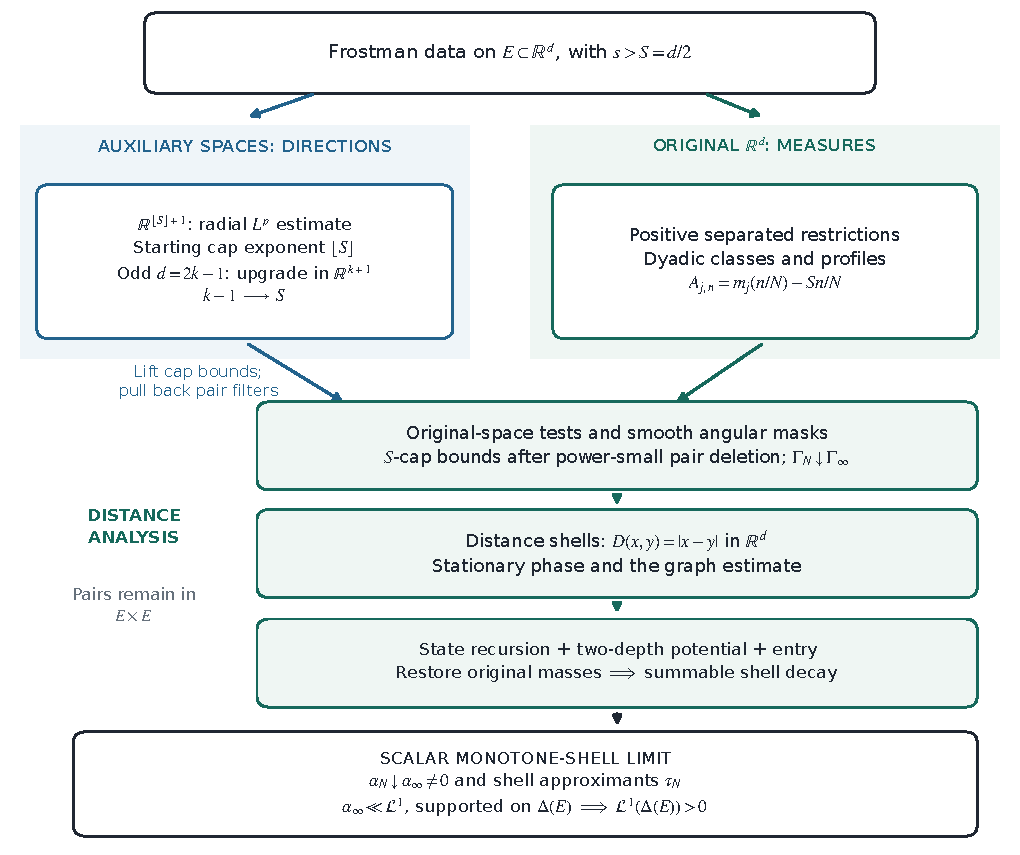
\includegraphics[width=\textwidth]{figures/proof-map.pdf}
 \caption{The main construction.
 Auxiliary projections prepare directional bounds and pair filters;
 the cap bounds hold after an additional power-small pair deletion.
 These data return to the original space, where the argument uses the
 Euclidean distance of the original pairs. The decreasing filters and
 shell-dependent approximants meet in the final scalar monotone-shell argument.}
 \label{fig:proof-map}
\end{figure}

\section{Conventions and preliminary facts}\label{sec:conventions}

\subsection{Measures, scales and directions}

All measures are finite Borel measures. A subprobability has mass at most
one. Restrictions are left unnormalized unless normalization is explicitly
specified. We write
\[
 I_s(\mu)=\iint |x-y|^{-s}\,\dd\mu(x)\dd\mu(y),
 \qquad
 \widehat\mu(\xi)=\int e^{-i x\cdot\xi}\,\dd\mu(x).
\]
For measures on the line we use the same Fourier convention.
The norm \(\|\cdot\|_{\TV}\) is total variation.
The notation \(f\lesssim g\) means \(f\le Cg\), with the dependence of \(C\)
specified by the ambient discussion.

A measure has an \(s\)-ball bound with loss \(K\), down to scale
\(\delta\), if
\[
 \mu(B(z,r))\le K r^s
 \quad\text{for every }z\text{ and }\delta\le r\le1.
\]
A cap bound on a sphere has the analogous meaning for its Euclidean
chordal metric. Passing between this metric, angular distance and fixed
smooth charts changes constants only. We may use dyadic radii, and enlarge
the constant to recover all radii in the specified interval.

For \(x\ne y\), put
\[
 \pi_x(y)=\frac{y-x}{|y-x|},\qquad D(x,y)=|x-y|.
\]
A tube is a neighborhood of an affine line; a plate is a neighborhood
of an affine plane of the dimension indicated. Directions are oriented
unless an antipodal pair of caps is explicitly used.
All configurations lie in bounded sets. Fixed rescalings and a finite
number of coordinate charts have constant cost.

The original ambient dimension is always denoted by \(d\), and
\(S=d/2\). We use \(R=2^N\) for the reciprocal final scale.
In odd dimension we write \(d=2k-1\); the linear angular gain is then used
in \(\R^{k+1}\), while \(S=k-1/2\) still refers to the original dimension.
Letters denoting dimensions inside a preliminary lemma are local to that
lemma.

\subsection{Finite energy and projection}

We record elementary consequences of the usual Frostman and projection
principles, including the restriction operation needed later.

\begin{lemma}\label{conv:energy}
Let \(\mu\) be supported in a bounded subset of \(\R^d\).
\begin{enumerate}[label=(\roman*)]
\item If \(\mu(B(z,r))\le C r^s\) for \(0<r\le1\), then
\(I_t(\mu)<\infty\) for every \(0<t<s\).
\item If \(I_t(\mu)<\infty\), then for every \(\eps>0\) there is a
compact restriction of mass at least \(\mu(\R^d)-\eps\) that satisfies
a \(t\)-ball bound with a finite constant.
\item If \(0<t<m\le d\), \(I_t(\mu)<\infty\), and \(P_V\) is
orthogonal projection to a Haar-random \(m\)-plane, then
\(I_t((P_V)_\#\mu)<\infty\) for almost every \(V\).
\end{enumerate}
\end{lemma}

\begin{proof}
For (i), split the integral at distance one and sum dyadic annuli.
The contribution at distance at most \(2^{-j}\) is bounded by
\(C2^{-j(s-t)}\), up to a constant depending on the total mass.

For (ii), let \(U_t^\mu(x)=\int |x-y|^{-t}\,\dd\mu(y)\).
This is finite for \(\mu\)-almost every \(x\), so a sufficiently large
level \(M\) discards arbitrarily little mass. Choose a compact subset
\(K\subset\{U_t^\mu\le M\}\) losing at most the remaining prescribed mass.
If \(K\cap B(z,r)\ne\varnothing\), choose \(x\) in this intersection.
Then
\[
 \mu|_K(B(z,r))
 \le\mu(B(x,2r))\le (2r)^t U_t^\mu(x)\le M(2r)^t.
\]
The same bound is immediate if the intersection is empty.

For (iii), rotational invariance and the integrability of the negative
\(t\)-moment of the length of an \(m\)-dimensional projection give
\[
 \int_{G(d,m)}|P_V z|^{-t}\,\dd V\le C_{d,m,t}|z|^{-t}
 \quad(z\ne0).
\]
For \(m<d\), this follows by integrating the density of the first \(m\)
coordinates of a uniform unit vector near zero: the radial integral there
is bounded by a constant times
\(\int_0^1 r^{m-1-t}\,\dd r<\infty\). For \(m=d\), the identity projection
makes the assertion immediate. Integrating in \((x,y)\) and applying
Tonelli proves the claim.
\end{proof}

We use Frostman's Lemma in its standard form
\cite[Theorem~8.8]{Mattila1995}: if a compact set \(E\)
has \(\dim_H E>s\), it supports a nonzero finite measure satisfying an
\(s\)-ball bound at all scales. Dividing by its mass gives a probability.
The positive dimension margin permits a slight decrease of \(s\) whenever
a finite energy rather than a ball bound is needed.

Dyadic cubes are half-open, so they form genuine partitions.
One may choose a translate of the dyadic grid whose boundaries have zero
mass for the finitely many starting measures: for each coordinate
hyperplane this follows by integrating its mass over the translation,
and the set of grid hyperplanes is countable.

\subsection{Subpower losses and fixed gains}

For a sequence \(R\to\infty\), a positive factor is at most subpower if it
is bounded by \(R^{o(1)}\). A retained mass is at least subpower if it is
bounded below by \(R^{-o(1)}\). These are statements about the sequence;
their use does not assert that an arbitrary fixed positive exponent is
zero. Constants and powers of \(\log R\) are subpower.
The corresponding notation for \(\delta\to0\) uses \(R=\delta^{-1}\).

We will use the following quantifier principle. It makes precise the
compactness passages in which the input losses tend to zero and an
argument produces a fixed positive improvement.

\begin{lemma}[Sequential uniformity principle]\label{conv:uniformity}
For fixed background parameters, let \(\mathcal C(\eps,R)\) be classes
of data, increasing in the allowed loss \(\eps>0\).
Let \(\mathcal G(c,R)\) be conclusions, weakening as the gain
\(c>0\) decreases. Suppose that for every sequence
\[
 \eps_j\downarrow0,\qquad R_j\to\infty,\qquad
 X_j\in\mathcal C(\eps_j,R_j),
\]
there are a subsequence and a fixed \(c>0\) on which
\(X_j\) satisfies \(\mathcal G(c,R_j)\) for all sufficiently large \(j\).
Then there exist \(\eps_0,c_0>0\) and \(R_0<\infty\) such that
every \(X\in\mathcal C(\eps_0,R)\), \(R\ge R_0\), satisfies
\(\mathcal G(c_0,R)\).
\end{lemma}

\begin{proof}
If the conclusion fails, for each \(j\) choose \(R_j\ge j\) and
\(X_j\in\mathcal C(1/j,R_j)\) failing \(\mathcal G(1/j,R_j)\).
The assumed subsequence satisfies \(\mathcal G(c,R_j)\) for some fixed
\(c>0\). For large \(j\), \(1/j<c\), so monotonicity implies
\(\mathcal G(1/j,R_j)\), a contradiction.
\end{proof}

Fixed constants in a power-small output may be absorbed by decreasing the
output exponent and increasing the scale threshold. When several losses
occur in an input, their maximum serves as \(\eps\) in
Lemma~\ref{conv:uniformity}. Compactness of uniformly Lipschitz normalized
profiles is the usual Arzel\`a--Ascoli compactness
\cite[Theorem~4.43]{Folland1999}.
All background parameters, including any strict dimension or
transversality exponent, are fixed before this principle is applied.
The detailed arguments below specify the required ordering of losses.

For measurable selection at a fixed scale it suffices to work with
dyadic grids, finite tube nets and a finite number of charts.
Strict inequalities can first be imposed with a fixed enlargement of
widths. Thus unions of exceptional configurations can be chosen Borel;
no selection from an uncountable unparameterized family is needed.

\section{Regularization and multiplication of fibre bounds}\label{reg:section}

We first record two finite-tree facts.  Neither requires lower density
estimates for the original measure.  Dyadic cubes are taken half open, so
that they form genuine measurable partitions; a fixed translation and
rescaling places each measure under consideration in one unit cube.
Related decompositions into dyadically regular measures occur in
\cite[Corollary~3.5]{KS2019}; we prove the version needed here.

\begin{lemma}[Regular classes]\label{reg:regularization}
Let $n\ge1$, let $\rho$ be a probability on a unit dyadic cube in
$\R^n$, and put $R=2^N$.  For every fixed $0<\lambda<1$ and all
sufficiently large $N$, there are pairwise disjoint sets $E_\alpha$,
each a union of depth-$N$ cubes, with the following properties:
\begin{enumerate}
\item Their number is at most $N^{C_n/\lambda}$, each has
      $\rho(E_\alpha)\ge R^{-\lambda}$, and
      \[
      \rho\Bigl(\R^n\setminus\bigcup_\alpha E_\alpha\Bigr)
      \le R^{-2}+N^{C_n/\lambda}R^{-\lambda}
      =R^{-\lambda+o(1)}.
      \]
\item For $\rho_\alpha=\rho|_{E_\alpha}/\rho(E_\alpha)$ there is a
      nondecreasing $n$-Lipschitz function $m_\alpha:[0,1]\to[0,n]$,
      with $m_\alpha(0)=0$, such that every occupied depth-$j$ cube
      satisfies
      \begin{equation}\label{reg:cell-mass}
      R^{-m_\alpha(j/N)-C_n\lambda}
      \le\rho_\alpha(Q)\le
      R^{-m_\alpha(j/N)+C_n\lambda},\qquad 0\le j\le N.
      \end{equation}
\item If $\rho(B(x,r))\le Kr^s$ for $R^{-1}\le r\le1$, with
      $0\le s\le n$ and $K\ge1$, then
      \begin{equation}\label{reg:profile-lower-bound}
      m_\alpha(u)\ge su-C_n\lambda-\log_R K,
      \qquad 0\le u\le1.
      \end{equation}
\end{enumerate}
Here and below an occupied cube means a cube of positive mass for the
specified class.  In particular, for occupied $P\subset Q$ at depths
$b\ge a$,
\begin{equation}\label{reg:conditional-mass}
\frac{\rho_\alpha(P)}{\rho_\alpha(Q)}
 =R^{-[m_\alpha(b/N)-m_\alpha(a/N)]\pm C_n\lambda}.
\end{equation}
Constants depend only on $n$; the threshold for $N$ can depend on
$\lambda$.
\end{lemma}

\begin{proof}
Discard depth-$N$ cubes of mass less than $R^{-n-2}$.  There are at most
$R^n$ such cubes, so this costs at most $R^{-2}$.  Choose depths
\[
0=j_0<j_1<\cdots<j_J=N,
\qquad j_i-j_{i-1}\le\lambda N+1,
\qquad J\le C/\lambda.
\]
Give each remaining leaf its dyadic mass bin as an initial label.  There
are $O_n(N)$ possible initial labels.  Work upwards through the selected
depths.  If $\ell$ is a label at depth $j_i$, count, within each
depth-$j_{i-1}$ parent, the depth-$j_i$ children carrying $\ell$; extend
$\ell$ by the dyadic bin of this positive count.  The extension is given
to all leaves of label $\ell$ in that parent.  A parent can carry
several labels, but the sets of leaves having different labels are
disjoint.  At every extension there are at most $O_n(N)$ possible count
bins.  Consequently the number of final labels is at most
$N^{C_n/\lambda}$, after adjusting constants for sufficiently large $N$.

Fix a final label.  For each $i$ there is a positive integer $b_i$,
which is a power of two, such that every occupied depth-$j_{i-1}$ parent
has between $b_i$ and $2b_i$ occupied depth-$j_i$ children in this label.
To check that these comparisons survive the later extensions, fix a
partial label and a node at the current selected depth. All leaves with
that label in this node receive the same extension, determined by its
parent and the old label. At each subsequent, higher step the extension
is again constant on this entire group. Backward induction through the
selected depths therefore shows that a final label retains or removes
each earlier child group as a whole; it never splits that group.
Consequently the branching comparisons hold simultaneously. Also
\[
1\le b_i\le 2^{n(j_i-j_{i-1})}.
\]
All leaf masses are in one dyadic bin.  Counting leaves below a selected
node, and then normalizing the final class, therefore gives
\[
\rho_\alpha(Q)=2^{\pm C J}
                  \Bigl(\prod_{h\le i}b_h\Bigr)^{-1}
\quad\text{at depth }j_i.
\]
Define
\[
m_\alpha(j_i/N)=\frac1N\sum_{h\le i}\log_2b_h
\]
and interpolate linearly.  Its slopes lie in $[0,n]$ exactly.  At an
intermediate depth, an occupied cube is contained in its preceding
selected-depth parent and contains an occupied descendant at the next
selected depth.  Both the possible mass variation and the profile
variation across this gap are at most $R^{n\lambda+O_n(1/N)}$.
The remaining comparison error is $2^{O(J)}$, whose base-$R$
logarithm is $O(1/(\lambda N))$.  For fixed $\lambda$ and sufficiently
large $N$ these errors imply Equation~\eqref{reg:cell-mass}.

Discard final classes of original mass less than $R^{-\lambda}$.
Their total mass is bounded by the number of labels times
$R^{-\lambda}$, as asserted.  For any retained class, normalization
multiplies an original upper ball bound by at most $R^\lambda$.
Covering a depth-$j$ cube by a bounded number of balls of radius
$2^{-j}$ gives
\[
\rho_\alpha(Q)\le C_nKR^\lambda2^{-sj}.
\]
Comparison with the lower bound in Equation~\eqref{reg:cell-mass}
proves Equation~\eqref{reg:profile-lower-bound} at integer depths,
with a larger dimensional constant.  Linear interpolation gives it at
every $u$.  Dividing two instances of Equation~\eqref{reg:cell-mass}
proves Equation~\eqref{reg:conditional-mass}.
\end{proof}

For use in scale-compactness arguments, the proof also gives the
following precise interpretation of subpower regularity.  If
$\lambda=\lambda_N\to0$ sufficiently slowly that
$\lambda_N^2N/\log N\to\infty$, then the number of classes, all mass
comparison losses, and the normalization losses of retained classes
are $R^{o(1)}$, while the discarded mass tends to zero.  Their
profiles remain exactly $n$-Lipschitz.  This
observation alone does not assert a fixed power of discarded mass:
fixed positive deletion exponents are obtained by choosing a fixed
small regularization parameter after the relevant compactness
argument.

\begin{lemma}[Density pruning and multiplication]\label{reg:pruning-multiplication}
Let $\rho$ be a source probability and $\nu$ a finite pin measure,
both on $\R^n$,
and let $0\le a_0<\cdots<a_J\le N$ be a fixed finite collection of
dyadic depths.  Suppose pin--source distances on the sets in question
are between fixed positive constants.  Let $G'$ be a measurable set of
pairs.  For each $j<J$, suppose there is a measurable set
$E_j\supset G'$ and a number $f_j\ge0$ such that every
$(x,z)\in G'$, with $z\in Q$ at depth $a_j$, satisfies
\begin{equation}\label{reg:local-fibre}
\rho\{z'\in Q\cap(E_j)_x:
     |\pi_x(z')-\pi_x(z)|\le C2^{-a_{j+1}}\}
 \le f_j\rho(Q).
\end{equation}
The constant $C$ may be any sufficiently large fixed constant,
depending on the geometry and on the fixed angular width to be used
below.  For every $e>0$ one can delete pair mass at most
$(J+1)R^{-e}\nu(\R^n)$ from $G'$ and obtain $G''$ such that, for each
pin $x$, each initial cube $Q_0$ at depth $a_0$, and every spherical
ball $B$ of radius $C_12^{-a_J}$,
\begin{equation}\label{reg:multiplied-fibre}
\rho\{z\in Q_0\cap G''_x:\pi_x(z)\in B\}
 \le R^{eJ}\Bigl(\prod_{j=0}^{J-1}f_j\Bigr)\rho(Q_0).
\end{equation}
An identical conclusion holds without a lower pin--source separation
if Equation~\eqref{reg:local-fibre} instead tests the perpendicular
distance to the full line $x+\R(z-x)$ at width $C2^{-a_{j+1}}$,
provided pin and source sets remain bounded and pairs on the diagonal
have been removed.
\end{lemma}

\begin{proof}
For each endpoint depth delete the pairs $(x,z)\in G'$ whose source
cube $Q$ satisfies
\[
\rho(Q\cap G'_x)<R^{-e}\rho(Q).
\]
For a fixed pin, the total source mass deleted at one depth is at most
$R^{-e}$, by summing over the disjoint cubes.  Integration in the pin
and a union bound prove the deletion estimate.  Notice that the
density condition concerns $G'$, before this last deletion.  No
density assertion for $G''$ is needed.

Fix $x,Q_0,B$.  Call a cube at any endpoint depth hit if it contains a
point of $Q_0\cap G''_x$ whose direction lies in $B$.  In a hit parent
$Q$ at depth $a_j$, choose one such point $z_Q$.  If a child $P$ at
depth $a_{j+1}$ is hit, choose a corresponding point $z_P$.  The map
$\pi_x$ is uniformly Lipschitz on the separated source set, so every
$z'\in P\cap G'_x$ has
\[
|\pi_x(z')-\pi_x(z_Q)|
 \le C_22^{-a_{j+1}}+2C_12^{-a_J}
 \le C2^{-a_{j+1}}.
\]
As $G'\subset E_j$, Equation~\eqref{reg:local-fibre} and the
pre-deletion density of every hit child imply
\[
\sum_{\substack{P\subset Q\\P\text{ hit at }a_{j+1}}}\rho(P)
 \le R^e\sum_{P\text{ hit}}\rho(P\cap G'_x)
 \le R^ef_j\rho(Q).
\]
Iterate this inequality from $Q_0$ to depth $a_J$.  The mass on the
left of Equation~\eqref{reg:multiplied-fibre} is at most the sum of the
full masses of the final hit cubes, proving that Equation.

For the line-width variant, the two hit witnesses have directions
within $2C_12^{-a_J}$.  Bounded pin--source distances from above imply
that $z_P$ lies within $O(2^{-a_J})$ of the line through $x,z_Q$;
every point of $P$ is then within $O(2^{-a_{j+1}})$ of that line.
The preceding argument applies unchanged.  This step uses no
Lipschitz bound for the radial map near its pin.
\end{proof}

All selections above can be made measurably: the cube partitions and
label sets are finite, and the fibre integrals are measurable.
Enlarging fixed test widths permits the use of closed caps or closed
tubes without altering any exponent.

\section{An angular projection gain}\label{ang:section}

This section proves the finite-scale incidence estimate used to improve
the angular exponent in odd dimensions. Its geometric content is a bound
on incidences whose fiber at each line direction is covered by a small
number of parallel tubes. The planar discretized Furstenberg theorem is
the only deep input.

All sets in this section lie in fixed bounded regions. Directions are unit
vectors, with antipodal vectors identified when discussing lines. A finite
number of projective charts removes this distinction. For a bounded set
$A$, write $|A|_r$ for its covering number by balls of radius $r$. A tube has
bounded length and the stated perpendicular width; enlarging its length by
a fixed constant is always permitted. We use the ball-bound and subpower
conventions of Section~\ref{sec:conventions}. Bounds for radii in a fixed
larger bounded interval follow by changing constants. In particular,
incidence mass at least subpower means a lower bound $\delta^{o(1)}$.

\subsection{The gain and its two slicing regimes}

\begin{theorem}[Linear projection gain]\label{ang:linear-gain}
Fix $k\ge2$ and
\[
 k-1\le q\le k-\tfrac12<t<k.
\]
Fix a tube-width constant $C$. In the case $q=k-1$, also fix
$\zeta>0$. There exist $\epsilon,c>0$ such that, for all sufficiently
small $\delta$, the following holds. Let $\mu$ be a bounded point
subprobability in $\R^{k+1}$ and $\nu$ a direction subprobability on $S^k$
with respective $t$- and $q$-ball bounds of loss $\delta^{-\epsilon}$
down to $\delta$. At $q=k-1$ assume in addition
\begin{equation}\label{ang:endpoint-plate}
 \nu\{w:\dist(w,H)\le r\}\le\delta^{-\epsilon}r^\zeta
       \qquad(\delta\le r\le1)
\end{equation}
for every linear hyperplane $H$. Let $E\subset\R^{k+1}\times S^k$ be a
measurable incidence relation, and write $E_w=\{x:(x,w)\in E\}$.
If each direction fiber $E_w$ is covered by at most
$\delta^{-q-\epsilon}$ tubes parallel to $w$ of width $C\delta$, then
\[
 (\mu\otimes\nu)(E)\le\delta^c.
\]
All constants are uniform over the measures and the incidence relations
with these fixed parameters.
\end{theorem}

A cover by $\delta^{-q-\epsilon}$ tubes means that the perpendicular
projection of a direction fiber is covered by that many balls of radius
comparable to $\delta$. The theorem says that such covers cannot capture
more than power-small incidence between the two nonconcentrated laws.

The two cases in its proof are distinguished by what remains after
slicing. If $q>k-1$, slicing by codimension $h=k-1$ leaves a plane and
exponents
\[
 b=q-h\in(0,\tfrac12],\qquad f=t-h\in(\tfrac12,1),\qquad b<f.
\]
The planar incidence estimate applies in this range. At $q=k-1$, the
same slicing would leave direction exponent zero. Instead we use
$h=k-2$, leaving three-dimensional slices with direction exponent one
and point exponent greater than $3/2$. The endpoint argument finds three
transverse directions in one such slice. A weak radial estimate with
exponent $\ell>k-2$ controls the triples that are almost dependent.

\subsection{The planar incidence input and its measure formulation}

The metric on bounded affine line parameters may be taken to be the sum
of the distance between the associated orthogonal projection operators
and the distance between the closest-to-origin points on the lines.
Other smooth bounded-chart metrics are equivalent. A nonempty bounded
set $P$ of points or line parameters is a $(\delta,s,K)$-set if
\[
 |P\cap B(a,r)|_\delta\le K r^s |P|_\delta
       \qquad(\delta\le r\le1).
\]
The normalization by $|P|_\delta$ is part of the defining bound.

\begin{theorem}[Planar discretized Furstenberg estimate]
\label{ang:furstenberg}
Let $0<b<1$ and $b<f<2$. There is $\epsilon_0>0$ such that the
following holds for sufficiently small $\delta$. Suppose that $P$ is
a nonempty bounded $(\delta,f,\delta^{-\epsilon_0})$-set and that
each $x\in P$ has a nonempty family $\mathcal T_x$ of incident
$\delta$-tubes whose line parameters form a
$(\delta,b,\delta^{-\epsilon_0})$-set. Then
\[
 \left|\bigcup_{x\in P}\mathcal T_x\right|_\delta
       \ge\delta^{-2b-\epsilon_0}.
\]
The exponent may be decreased to absorb fixed bounded charts and fixed
width multiples.
\end{theorem}

This is the tube formulation in
\cite[Definitions~2.5--2.6 and Theorem~2.7]{OSW2024}, following the
discretized theorem of \cite[Theorem~1.3]{OS2023}. In the application
below, $f<1$; that range is included in the theorem.

The measure formulation below keeps the labels being sampled separate
from their geometric coordinates. Several labels may have the same
coordinate and still carry different incidence fibers.

\begin{lemma}[Planar measure incidence obstruction]
\label{ang:planar-measures}
Fix $0<b<1$ and $b<f<2$. There is no sequence $\delta\to0$ with the
following data. Let $\mu,\nu$ be subprobabilities on Borel label sets
$X,W$ in Euclidean spaces, and let
\[
 p:X\longrightarrow\R^2,\qquad v:W\longrightarrow S^1
\]
be measurable coordinate maps with fixed bounded images. Suppose that
$p_\#\mu$ and $v_\#\nu$ have respective $f$- and $b$-ball bounds
of loss $\delta^{-o(1)}$ down to $\delta$. Let $E\subset X\times W$ be a measurable
incidence relation with
\[
 (\mu\otimes\nu)(E)\ge\delta^{o(1)}.
\]
For each original direction label $\omega\in W$, put
$E_\omega=\{\xi\in X:(\xi,\omega)\in E\}$. Assume that the set of
point coordinates $p(E_\omega)$ is covered by at most
$\delta^{-b-o(1)}$ strips of width $C\delta$ parallel to $v(\omega)$.
\end{lemma}

\begin{proof}
Restrict the coordinate images to fixed bounded charts and normalize the
two laws. Their masses are at least the incidence mass, so this costs only
subpower factors. Let $I$ be the resulting incidence mass, sample
$n=\lceil\delta^{-b}\rceil$ independent direction labels
$\omega_1,\ldots,\omega_n$ from $\nu$, and write $v_i=v(\omega_i)$.
There is a subpower quantity $T\to\infty$ such that, with failure
probability smaller than any prescribed power of $\delta$, the sample
satisfies
\begin{equation}\label{ang:sample-caps}
 \#\{i:v_i\in B(v_0,r)\}\le Tnr^b
       \qquad(\delta\le r\le1).
\end{equation}
To verify this, use a fixed collection of dyadic grids in the direction
chart. There are only polynomially many relevant cells. Their expected
counts are at most $Knr^b$, where $K=\delta^{-o(1)}$, and
$nr^b\ge1$. Choose $T$ larger than a fixed large multiple of
$K+\log(1/\delta)$. For a binomial count $Y$, the bound
\[
 \Pr(Y\ge j)\le (e\mathbb E Y/j)^j
\]
and a union bound prove Equation~\eqref{ang:sample-caps}, including
arbitrary balls by fixed grid comparison. Increasing $T$ by another
subpower factor makes the failure probability smaller than $I/4$.

The expected empirical incidence mass equals $I$. Since it is bounded
by one, there exists a sample satisfying Equation~\eqref{ang:sample-caps}
and having empirical incidence mass at least $I/2$. The set $X_0$ of
point labels incident to at least $In/4$ sampled direction labels has
$\mu$-mass at least $I/4$: its complement contributes at most $I/4$
to the empirical incidence integral. Normalize $\mu|_{X_0}$ and sample
$m=\lceil\delta^{-f}\rceil$ independent point labels. If their coordinates
are $x_1,\ldots,x_m$, the same argument gives a sample with
\[
 \#\{j:x_j\in B(x,r)\}\le T'mr^f,
 \qquad T'=\delta^{-o(1)},\qquad \delta\le r\le1.
\]
In particular, the multiplicities in $\delta$-balls are subpower.
Color a spatial $\delta$-grid with finitely many colors so that cells
with the same color are $\delta$-separated. Choose a color with the most
occupied cells and one sampled label from each of them. Their
point coordinates form a separated set $P$ with
$|P|_\delta\ge m\delta^{o(1)}$. The displayed local count makes $P$
a $(\delta,f,\delta^{-o(1)})$-set. Each $x\in P$ retains the list of at
least $In/4$ good sampled direction labels belonging to its chosen point
label.

For $x\in P$, take the lines exactly through $x$ in the coordinates
$v_i$ of those listed labels, and let $\mathcal T_x$ be their
$\delta$-tubes. Equation~\eqref{ang:sample-caps} bounds the multiplicity
in a $\delta$-ball of directions by $CT$, and the count in an $r$-ball
by $Tnr^b$. Consequently
\[
 |\mathcal T_x|_\delta\ge cIn/T,
 \qquad
 |\mathcal T_x\cap B(\ell,r)|_\delta\le CTnr^b.
\]
Here the direction component of the line metric supplies the lower
distance comparison; the reverse comparison holds because $x$ is bounded.
The normalized loss is therefore at most $CT^2/I=\delta^{-o(1)}$.
In particular, $\mathcal T_x$ is a nonempty
$(\delta,b,\delta^{-o(1)})$-set of line parameters even when different
sampled labels have the same direction coordinate.

For each sampled label $\omega_i$, its prescribed strips contain the
coordinates of all its incident sampled point labels. Moving the central
line of such a strip to pass through one of these points changes its
intercept by $O(\delta)$. Thus each original strip accounts for only a
bounded number of $\delta$-cells in line-parameter space. Altogether the
union of our line families has covering count at most
\[
 n\delta^{-b-o(1)}=\delta^{-2b-o(1)}.
\]
This contradicts Theorem~\ref{ang:furstenberg} for small $\delta$.
The count treats each original sampled direction label separately; it
never asks for one common fiber cover after coincident coordinates are
identified.
\end{proof}

\subsection{Slicing with controlled losses}

We state the needed estimates for Haar-random subspaces before applying
them. Haar measure is normalized to have total mass one.

\begin{lemma}[Haar band estimates]\label{ang:haar}
Let $0\le h\le n-1$, and let $V$ be a Haar-random codimension-$h$
linear subspace of $\R^n$.
For a unit vector $w$,
\[
 \Pr\{\dist(w,V)\le\delta\}\asymp\delta^h.
\]
If $j\le n-h$ unit vectors $w_1,\ldots,w_j$ have singular values
$d_1\ge\cdots\ge d_j\ge0$, then
\begin{equation}\label{ang:haar-multiple}
 \delta^{-jh}\Pr\{\dist(w_i,V)\le\delta\text{ for all }i\}
       \le C_{n,j}\prod_{i=1}^j(d_i+\delta)^{-h}.
\end{equation}
When $h=0$, the probability and the factors with exponent $h$ are one.
\end{lemma}

\begin{proof}
The one-vector estimate follows from spherical coordinates. For the
second estimate, singular-value decomposition implies that the band
conditions constrain the projections of orthonormal singular directions
$u_i$ by $C_j\delta/d_i$. Keep only the constraints whose right-hand
sides are less than a sufficiently small dimensional constant, and
order these right-hand sides increasingly. By rotational invariance,
one can fix $V^\perp$ and reveal successive vectors of a random
orthonormal frame. Conditional on the earlier constrained vectors,
projection onto $V^\perp$, restricted to their orthogonal complement,
has rank $h$ and nonzero singular values bounded below. Indeed the sum
of squared lengths of the earlier projections is less than $1/2$ if
the dimensional constant was chosen small enough. The next vector is
uniform on the unit sphere of that complement. Its probability of
having projection of length at most $r$ is at most $C_n r^h$.
The ambient dimension at this last conditional step is at least
$n-j+1\ge h+1$, including the limiting case of a one-dimensional
kernel. Multiplying the conditional estimates proves
\[
 \Pr\{w_i\text{ all in the band}\}
       \le C_{n,j}\prod_i\min(1,\delta/d_i)^h,
\]
which is equivalent to Equation~\eqref{ang:haar-multiple}.
\end{proof}

Shmerkin and Wang \cite[Sections~6.1--6.3]{SW2025} use normalized bands
to define slices and combine sliced with projected thin-tube bounds.
Here we keep bands at width $\delta$ and control the retained incidence
mass, ball bounds, and active tubes for each original direction label.

\begin{lemma}[Selection of slices]\label{ang:slice-selection}
Let $0\le h\le n-2$. Let point and direction subprobabilities $\mu,\nu$ in $\R^n$ have
$t$- and $q$-ball bounds with subpower losses, where $t,q>h$.
Assume the directions lie in a fixed small projective chart. Let an
incidence relation $E$ have mass at least subpower, and suppose each
direction fiber is covered by at most $\delta^{-q-o(1)}$ tubes of
width $C\delta$.

For Haar-random codimension-$h$ subspaces $V$ and
$z\in V^\perp$, set
\begin{align*}
 d\nu_V(w)&=\delta^{-h}\one_{\{|P_{V^\perp}w|\le\delta\}}\,d\nu(w),\\
 d\mu_{V,z}(x)&=\delta^{-h}
       \one_{\{|P_{V^\perp}x-z|\le\delta\}}\,d\mu(x).
\end{align*}
Integrate $z$ over a fixed sufficiently large ball. There are families of restrictions
$\widetilde\nu_V\le\nu_V$, $\widetilde\mu_{V,z}\le\mu_{V,z}$,
and relations $\widetilde E_{V,z}\subset E$, measurable in the displayed
parameters and restricted to the two bands defining $\mu_{V,z}$ and
$\nu_V$, such that
\[
 \mathbb E_V\int
 (\widetilde\mu_{V,z}\otimes\widetilde\nu_V)(\widetilde E_{V,z})\,dz
 \ge\delta^{o(1)},
\]
and the following hold:
\begin{enumerate}
\item The restricted measures have masses and ball losses at most
$\delta^{-o(1)}$, with exponents $q-h$ and $t-h$, respectively.
\item Each remaining direction fiber is covered by at most
$\delta^{-(q-h)-o(1)}$ width-$C'\delta$ tubes.
\item Put
\[
 p_{V,z}(x)=P_Vx,\qquad v_V(w)=P_Vw/|P_Vw|
 \quad\text{for }|P_{V^\perp}w|\le\delta.
\]
The first map is projection to $V+z$ followed by translation to $V$;
the second is well-defined on the direction band for small $\delta$.
The coordinate pushforwards of the restricted measures under these maps
satisfy the ball bounds in item~1, with fixed constant changes. For every
original direction label $w$ in that band, the coordinates
$p_{V,z}(\{x:(x,w)\in\widetilde E_{V,z}\})$ have the tube cover in
item~2 with direction $v_V(w)$. This cover remains attached to $w$ even
when two projected direction coordinates coincide.
\end{enumerate}
The direction restriction $\widetilde\nu_V$ depends on $V$ only, and its
mass has an a priori subpower upper bound valid for every $V$.
\end{lemma}

\begin{proof}
We first choose the fiber covers measurably, enlarging their width by a
fixed dimensional factor while preserving each actual direction $w$.
Let $M_\delta=\delta^{-q-o(1)}$ be their common size bound. Use a finite
spatial $\delta$-grid in a fixed bounded region containing one point on
every axis whose tube meets the source region. Rounding such a point
to the grid and keeping the direction $w$ enlarges the width by only
$C_n\delta$. Candidate covers are the finitely many lists of at most
$\lfloor M_\delta\rfloor$ grid anchors. For each candidate $J$, the
function
\[
 w\longmapsto
 \mu\left(E_w\setminus\bigcup_{a\in J}T(w,a)\right)
\]
is measurable by Fubini, where $T(w,a)$ is the enlarged tube parallel
to $w$ through $a$. Choose the first candidate for which this function
is zero. Coverage up to a $\mu$-null set suffices, since every point
slice $\mu_{V,z}$ is absolutely continuous with respect to $\mu$.
For a relation measurable only in the completed product sigma-algebra,
first choose a Borel subset agreeing with the relation modulo a
product-null set, and discard the $\nu$-null set of
directions on which its fiber differs by positive $\mu$-mass. Every
direction slice is absolutely continuous with respect to $\nu$, so
this replacement also changes no sliced incidence.
Writing $J(w)$ for the selected candidate, now replace $E$ by
\[
 E\cap\left\{(x,w):x\in\bigcup_{a\in J(w)}T(w,a)\right\},
\]
with the exceptional null directions removed. This loses zero original
or sliced incidence and makes the selected covers contain every fiber
of the restricted relation.

Intersecting the relation with the two bands does not change its sliced
incidence. The expected sliced incidence is comparable from below to the
original one. In fact, integrating the point-band indicator in $z$ gives a
constant times $\delta^h$, and the one-vector Haar estimate supplies
another factor comparable to $\delta^h$. These cancel the two slice
normalizations.

Write $M(V)=\|\nu_V\|$ and $L(V,z)=\|\mu_{V,z}\|$.
Uniformly in $V$,
\begin{equation}\label{ang:point-slice-total}
 \int L(V,z)\,dz\le C.
\end{equation}
The two-vector estimate in a projective chart gives the direction-pair
kernel
\begin{equation}\label{ang:direction-pair-kernel}
 \delta^{-2h}\Pr\{w,w'\text{ both within }\delta\text{ of }V\}
       \le C(|w-w'|+\delta)^{-h}.
\end{equation}
For points, integrate both band indicators in $z$ first. This yields
at most $C\delta^h$ times the indicator
$|P_{V^\perp}(x-x')|\le2\delta$. Haar averaging therefore gives
the analogous normalized kernel $C(|x-x'|+\delta)^{-h}$.
Dyadic annulus summation, using $q,t>h$, proves
\begin{align}
 \mathbb E_V M(V)^2+\mathbb E_V\int L(V,z)^2\,dz
       &\le\delta^{-o(1)},\label{ang:slice-second}\\
 \mathbb E_V\iint_{|w-w'|\le r}d\nu_V(w)d\nu_V(w')
       &\le\delta^{-o(1)}r^{q-h},\label{ang:direction-close}\\
 \mathbb E_V\int\iint_{|x-x'|\le r}
             d\mu_{V,z}(x)d\mu_{V,z}(x')\,dz
       &\le\delta^{-o(1)}r^{t-h}\label{ang:point-close}
\end{align}
for $\delta\le r\le1$. For example, the shells below $r$ form a
geometric sum with successive exponents $q-h>0$ in
Equation~\eqref{ang:direction-close}; the finest shell uses the
original ball estimate at radius $\delta$.

The truncations below first bound direction-slice mass, then enforce
both ball bounds, and finally bound the active tube count. Take a subpower number
$K\to\infty$ absorbing all constants, all input losses, the dyadic
radius sums in Equations~\eqref{ang:direction-close} and
\eqref{ang:point-close}, and the inverse original incidence mass.
Enlarge it so the sliced incidence is at least $K^{-1}$ and the
right-hand side of Equation~\eqref{ang:slice-second} is at most $K$.
First remove planes with $M(V)>K^3$. By
Equations~\eqref{ang:point-slice-total} and \eqref{ang:slice-second},
their incidence contribution is at most $CK^{-2}$.

In the remaining point slices, remove points at which
\[
 \mu_{V,z}(B(x,Cr))>K^6r^{t-h}
\]
at some dyadic radius $r\in[\delta,1]$. Markov's inequality and
Equation~\eqref{ang:point-close} bound the expected deleted point mass
by $CK^{-5}$. Since $M(V)\le K^3$, its incidence cost is at most
$CK^{-2}$. The restricted point measure has the asserted ball bound
at every center: any ball meeting the retained set can be enlarged
by a fixed factor around a retained point. It also has mass $O(K^6)$,
by covering the bounded support with a fixed number of unit balls.

Similarly remove direction-slice points for which
$\nu_V(B(w,Cr))>K^3r^{q-h}$ at some dyadic radius. Their expected
mass is at most $CK^{-2}$ by
Equation~\eqref{ang:direction-close}; Equation~\eqref{ang:point-slice-total}
bounds the corresponding integrated incidence loss by the same quantity.
No independence between direction mass and point mass is used here.

Finally, for a direction $w$ in the band about $V$, let $J(w)$ be its
selected list of grid anchors. A bounded tube through $a$, parallel to
$w$, can meet the source region in the band about $V+z$ only if
$|P_{V^\perp}a-z|\le C'\delta$: its transverse projection within the
bounded source region has diameter $O(\delta)$. Thus the measurable
upper count
\[
 N(V,z,w)=\sum_{a\in J(w)}
       \one_{\{|P_{V^\perp}a-z|\le C'\delta\}}
\]
dominates the number of active covering tubes and satisfies
\[
 \int N(V,z,w)\,dz
       \le C M_\delta\delta^h\le K\delta^{h-q}.
\]
Delete direction/$z$ pairs for which
$N(V,z,w)>K^{12}\delta^{h-q}$. Their $z$-volume for each $V,w$
is at most $K^{-11}$. The truncated point mass is $O(K^6)$ and
the truncated direction mass is at most $K^3$, so this costs at most
$CK^{-2}$ in integrated incidence. Delete the corresponding incidences
but keep the marginal restrictions already constructed. At large $K$
the surviving integrated incidence is at least $(2K)^{-1}$.

Projection changes each direction by $O(\delta)$. The points of one
band whose coordinates $p_{V,z}(x)$ lie in a ball of radius $r\ge\delta$
lie in a ball of radius $Cr$ in the original space; the same assertion
holds for directions after unit normalization. These preimage bounds give
the asserted ball bounds on the coordinate pushforwards. For each original
label $w$, every active tube in its own selected list becomes a tube of
width $C'\delta$ parallel to $v_V(w)$. This proves item~3 for each
original direction label.
\end{proof}

\subsection{Endpoint preparation: transverse tubes and weak radial estimates}

We first record the elementary counting fact used twice below.

\begin{lemma}[Transverse tube counting]\label{ang:loomis-whitney}
Let $v_1,\ldots,v_m$ be unit vectors in $\R^m$, $m\ge2$, and suppose
$|\det(v_1,\ldots,v_m)|\ge\Delta>0$. If a bounded set $A$ is covered,
for each $i$, by $M_i$ tubes of width $C\delta$ parallel to $v_i$, then
\[
 |A|_{C_m\delta}\le C_{m,C}\Delta^{-m}
       \prod_{i=1}^m M_i^{1/(m-1)}.
\]
Changing the fixed constant in the covering radius changes only the
constant in this inequality.
\end{lemma}

\begin{proof}
Let $L$ be the matrix with columns $v_i$. Then $\|L\|\le C_m$ and
$\|L^{-1}\|\le C_m\Delta^{-1}$. Let $S\subset\Z^m$ index the
$\delta$-grid cubes meeting $L^{-1}A$. The image of such a cube has
diameter at most $C_m\delta$. Each original tube parallel to $v_i$
becomes a tube parallel to the $i$th coordinate axis, of width at most
$C_{m,C}\delta\Delta^{-1}$. Therefore
\[
 |\operatorname{pr}_{\widehat i}S|
       \le C_{m,C}\Delta^{-(m-1)}M_i.
\]
The discrete Loomis--Whitney inequality \cite{LoomisWhitney1949}
$|S|^{m-1}\le\prod_i|\operatorname{pr}_{\widehat i}S|$ proves the
claim. For completeness, if $X$ is uniform on $S$, the entropy chain rule
gives
\[
 H(X_{\widehat i})\ge
 \sum_{j\ne i}H(X_j\mid X_1,\ldots,X_{j-1}).
\]
Summing in $i$ yields $(m-1)\log|S|\le
\sum_i\log|\operatorname{pr}_{\widehat i}S|$, as required.
\end{proof}

For $x\ne z$, put $\pi_x(z)=(z-x)/|z-x|$. A restriction of the
product measure to a pair set is not normalized in the next statement.

\begin{lemma}[Weak radial estimate]\label{ang:weak-radial}
Fix $k\ge2$, $\zeta>0$, and
\[
 k-2<\ell<\frac{(k-1)^2}{k}.
\]
For every $e>0$ there exist $\epsilon,c>0$ with the following property
for sufficiently small $\delta$. Suppose that a probability $\lambda$
in a bounded subset of $\R^k$ satisfies
\begin{align*}
 \lambda(B(x,r))&\le\delta^{-\epsilon}r^{k-1},\\
 \lambda(H^{(r)})&\le\delta^{-\epsilon}r^\zeta
 \qquad(\delta\le r\le1)
\end{align*}
for every affine hyperplane $H$, where $H^{(r)}$ is its $r$-neighborhood.
There is a measurable pair set $G$ such that
\[
 (\lambda\otimes\lambda)(G^c)\lesssim\delta^c,
 \qquad
 \lambda\{z:(x,z)\in G,\ \pi_x(z)\in B(\theta,r)\}
       \le\delta^{-e}r^\ell
\]
for every $x$, every spherical cap center $\theta$, and
$\delta\le r\le1$. The diagonal is omitted from $G$. The conclusion
also holds for balls in projective direction space, with a fixed change
of constant, by taking the two antipodal caps.
\end{lemma}

\begin{proof}
We first prove a single-scale assertion at $u=2^{-N}$, with reciprocal
scale $R=2^N$: for any fixed $\ell_1<(k-1)^2/k$, sufficiently small
fixed losses in the hypotheses permit deletion of $O(R^{-c_1})$ pair
mass so that every remaining fiber has cap mass at most $R^{-\ell_1}$
at radius $u$. All choices made below are fixed independently of $R$.

Apply Lemma~\ref{reg:regularization} to the source measure with a small
parameter $\tau>0$. It suffices to treat one normalized source class
$\rho$, retaining the original pin law $\lambda$. The discarded source
mass is a fixed negative power of $R$, and the classes will be recombined
with their original weights. Write $m$ for the class profile. Its
comparison errors are $R^{C_k\tau}$, it is $k$-Lipschitz, and
\[
 m(1)\ge k-1-C_k\tau-\epsilon.
\]
The constant absorbs the normalization of a class of mass at least
$R^{-\tau}$. At depths $a<b$, an occupied depth-$b$ child of an
occupied depth-$a$ cell $Q$ has conditional $\rho$-mass at most
\begin{equation}\label{ang:conditional-child}
 R^{C_k\tau}D^{-1},\qquad
 D=R^{m(b/N)-m(a/N)}.
\end{equation}

Divide the depth interval into $J$ nearly equal blocks, with $J$ a
large fixed integer, and ignore the first two blocks. In every later
block $[a,b]$, remove the pairs whose pin is within $R^{-1/(4J)}$ of
the center $z_Q$ of the source cell $Q$ at depth $a$. Summing with the
source-cell weights shows that this costs at most
$C_JR^{-(k-1)/(4J)+\epsilon}$ pair mass. For the other pairs the center
direction
\[
 v(x,Q)=\frac{z_Q-x}{|z_Q-x|}
\]
differs from the direction to any point of $Q$ by
$O(2^{-a}R^{1/(4J)})$. In particular the transverse displacement inside
$Q$ caused by freezing this direction is
\begin{equation}\label{ang:freezing-error}
 O(2^{-2a}R^{1/(4J)})=o(2^{-b});
\end{equation}
here $a\ge2N/J+O(1)$ and $b-a=N/J+O(1)$.

Fix a small $e'>0$. A pair $(x,z)$, $z\in Q$, is troublesome if the
full conditional source mass in the width-$C2^{-b}$ tube about the
line through $x,z$ exceeds
\begin{equation}\label{ang:local-fraction}
 F=R^{e'}D^{-(k-1)/k}.
\end{equation}
The fixed width $C$ may be chosen as large as any subsequent application
requires. If $F\ge1$, there are no troublesome pairs. Otherwise,
Equation~\eqref{ang:freezing-error} and a grid in $v(x,Q)^\perp$ show
that all troublesome sources for this pin lie in at most $C/F$
parallel tubes of width $C'2^{-b}$. Indeed, each relevant projected grid
cell has a fixed enlargement of conditional mass greater than $F$;
these enlargements have bounded overlap.

For this fixed $Q$, let $B_x$ be its troublesome source set when the
pin survives the near-pin deletion, and let $B_x=\varnothing$ otherwise.
Put $\rho_Q=\rho|_Q/\rho(Q)$ and
\[
 I_Q=\int\rho_Q(B_x)\,d\lambda(x).
\]
We claim that $I_Q\le R^{-c_2}$, uniformly in $Q$. Suppose instead that
$I_Q\ge R^{-c_2}$. Jensen's inequality, applied to the pin-incidence
mass at each source, gives
\begin{equation}\label{ang:common-k-incidence}
 \int \rho_Q\Bigl(\bigcap_{i=1}^k B_{x_i}\Bigr)
           \,d\lambda(x_1)\cdots d\lambda(x_k)
      \ge I_Q^k.
\end{equation}
Tuples containing a removed pin contribute zero to this integral. For a
tuple of surviving pins, if
$|\det(v(x_1,Q),\ldots,v(x_k,Q))|<R^{-\eta}$, one of the
successive Gram--Schmidt distances is less than
$R^{-\eta/(k-1)}$. Conditional on the preceding pins, the corresponding
pin lies in a $C R^{-\eta/(k-1)}$-neighborhood of an affine hyperplane
through $z_Q$. Thus the product measure of these tuples is at most
\[
 C_kR^{\epsilon-\eta\zeta/(k-1)}.
\]
Choose $\eta$ small compared with $e'$, and then choose
$c_2,\epsilon$ so small that this is $o(R^{-kc_2})$. There is a tuple
of determinant at least $R^{-\eta}$ whose common source set has
conditional mass at least $\tfrac12R^{-kc_2}$. By
Equation~\eqref{ang:conditional-child}, it needs at least
\[
 c D R^{-kc_2-C_k\tau}
\]
balls of radius comparable to $2^{-b}$. On the other hand,
Lemma~\ref{ang:loomis-whitney}, applied to its $k$ tube covers, bounds
this number by
\[
 C D R^{k\eta-e'k/(k-1)}.
\]
The two estimates are contradictory if
\[
 k\eta+kc_2+C_k\tau<\frac{ke'}{k-1}.
\]
These parameter requirements are compatible: first choose $\eta$,
then $c_2$, and finally $\tau,\epsilon$. This proves the claim.
Deleting troublesome pairs and summing over $Q$ costs at most
$R^{-c_2}$ per block, because the weights $\rho(Q)$ sum to one.

Apply the endpoint density pruning of
Lemma~\ref{reg:pruning-multiplication}, with an additional loss
$R^{e''}$ per block, to the surviving pair set. Its physical-tube
version applies even though pins need not be separated from sources
by a fixed constant. To check this point directly, fix a parent $Q$ and
consider its depth-$b$ children meeting one final cap of radius
$2^{-N}$. Every point of such a child is within $C2^{-b}$ of the
target line. Choose one retained witness in one hit child of $Q$.
Its line differs from the target line by transverse distance
$O(2^{-N})$ in the bounded source region. Thus the pre-density-deletion
survivors in all hit children of this parent satisfy the same local
test at width $C'2^{-b}$. In each child their mass is at least
$R^{-e''}$ times the full child mass. The one local fraction bound
therefore charges the sum of the full masses of hit children by
$R^{e''}F$ times the full parent mass. It uses the
survivor set before the final density deletion; no renewed density
claim after that deletion is needed.

Multiplying these inequalities telescopes the profile increments.
Sum the resulting bounds over the occupied initial cells at the end of
the two ignored blocks. Their masses sum to one, so this introduces no
factor equal to the number of cells. The ignored growth is at most
$2k/J+o(1)$. Consequently every final cap has normalized class mass at most
\[
 R^{J(e'+e'')+o(1)}
 R^{-\frac{k-1}{k}(k-1-2k/J-C_k\tau-\epsilon)}.
\]
Choose $J$ large depending on $(k-1)^2/k-\ell_1$, then $e',e''$
small, and then the remaining losses as above. This proves the
single-scale assertion. All deletion exponents are positive fixed
numbers. Recombining classes with their original weights preserves
the cap estimate and the power deletion; the negligible discarded
class mass is included in the deletion.

Now choose $\ell<\ell_1<(k-1)^2/k$. It is enough to consider
$0<e<1$. Apply the single-scale assertion at dyadic $u$ between
$\delta$ and $\delta^{e/(2k)}$. At these scales the input loss
$\delta^{-\epsilon}$ is at most $u^{-2k\epsilon/e}$, so choosing
$\epsilon$ sufficiently small makes all the single-scale hypotheses
uniformly valid. The sum of the deletions is at most
\[
 C\log(1/\delta)\,\delta^{ec_1/(2k)},
\]
which is a positive power of $\delta$ after decreasing its exponent.
Intersect the surviving pair sets. Dyadic comparison gives the desired
cap estimate for $r\le\delta^{e/(2k)}$; the slack between $\ell$
and $\ell_1$ absorbs fixed constants. For larger $r$,
$\delta^{-e}r^\ell\ge1$ at small scales, so the estimate is trivial.
This completes the proof.
\end{proof}

\subsection{Proof of the linear gain}

\begin{proof}[Proof of Theorem~\ref{ang:linear-gain}]
We rule out any sequence with subpower input losses, subpower incidence
mass from below, and cover size $\delta^{-q-o(1)}$. This implies the
stated fixed-power result: if no positive $\epsilon,c$ worked, choose
counterexamples with $\epsilon=c=1/j$ at scales
$\delta_j<1/j$ tending to zero. They would form precisely such a
sequence. This observation will also justify all uses of the gain with
sufficiently small fixed losses.

By choosing one of finitely many small projective charts, we can assume
all relevant directions lie in a single chart and that incidence still
has subpower mass. If $q>k-1$, apply
Lemma~\ref{ang:slice-selection} with $h=k-1$. Select a slice with
subpower incidence and normalize its marginal restrictions; their
masses are bounded above by subpower and below by the incidence divided
by the other marginal mass. The coordinate maps take values in a plane, with
\[
 b=q-h\in(0,\tfrac12],\qquad
 f=t-h\in(\tfrac12,1),\qquad b<f,
\]
and tube count at most $\delta^{-b-o(1)}$. Apply
Lemma~\ref{ang:planar-measures} with the original sliced points and
directions as labels, and with coordinate maps $p_{V,z}$ and $v_V$.
Item~3 of Lemma~\ref{ang:slice-selection} gives the ball bounds on their
coordinate pushforwards and the separate cover for each original direction
label. The labeled incidence relation still has subpower mass, so these
data contradict the planar obstruction.

At $q=k-1$, slicing to the plane would leave direction exponent zero,
outside the range of Lemma~\ref{ang:planar-measures}. We therefore put
$h=k-2$, so the selected slices have dimension three, and let
\[
 g=t-h-\tfrac32>0.
\]
Choose once and for all $0<a<g/4$. We will find in one slice three
directions of determinant at least $c\delta^a$ with a common incident
point set of mass at least subpower. The resulting loss in
Lemma~\ref{ang:loomis-whitney} is $O(\delta^{-3a})$, which the
strict gap $g$ will absorb.

Parameterize our chart by $p\in\R^k$, with unit direction
$w(p)=(1,p)/\sqrt{1+|p|^2}$. Restricting and normalizing the chart
costs only a subpower factor; denote the resulting law in $p$ by
$\lambda$. In the rest of the endpoint proof the direction law supplied
to slicing is $w_\#\lambda$, and the incidence relation is restricted to
this chart. The slice law of the chart labels is
\[
 d\lambda_V(p)=\delta^{-h}
 \one_{\{|P_{V^\perp}w(p)|\le\delta\}}\,d\lambda(p),
 \qquad \nu_V=w_\#\lambda_V.
\]
Equation~\eqref{ang:endpoint-plate}
becomes the affine-hyperplane bound in the $p$ coordinates, because
an affine hyperplane there is the intersection of a linear hyperplane
with the chart. The ball exponent remains $k-1$. Choose
\[
 h<\ell<\frac{(k-1)^2}{k}=h+\frac1k.
\]
Apply Lemma~\ref{ang:weak-radial} to this chart law, with a small
fixed output loss $\delta^{-e}$. Its hypotheses hold at sufficiently
small scales for every fixed input-loss threshold. This deletes a
pair set of original product mass $O(\delta^{c_e})$ and gives, for
every anchor $p$, an $\ell$-cap bound $\delta^{-e}r^\ell$ on
the undeleted displacement directions. Also delete pairs at distance
less than $\delta^{b_0}$, where $b_0>0$ will be small. Denote the union
of these two exceptional pair relations by $\mathcal E_{\mathrm{pair}}$,
and call an anchored pair retained when it lies outside this union.

We first record how these deletions transfer to normalized slice-pair
mass. Equation~\eqref{ang:direction-pair-kernel}
shows that for every measurable chart-pair relation $\mathcal E$ with
$(\lambda\otimes\lambda)(\mathcal E)\le\delta^c$, and every fixed
$\theta>0$,
\begin{equation}\label{ang:exceptional-pair-transfer}
 \mathbb E_V(\lambda_V\otimes\lambda_V)(\mathcal E)
 \le C\delta^{c-\theta h}
       +\delta^{\theta(q-h)-o(1)}.
\end{equation}
For $0<\theta\le1$, the first term treats distances greater than
$\delta^\theta$, and the second treats smaller distances by the ball
bound and annular summation. For $\theta\ge1$, the kernel is at most
$C\delta^{-h}$, so the whole expectation is at most
$C\delta^{c-h}\le C\delta^{c-\theta h}$. The same annulus calculation
bounds the expected mass of the close pairs by
$\delta^{b_0(q-h)-o(1)}$. We leave $\theta$ free until $e$, and hence
the weak-radial deletion exponent $c_e$, has been fixed.

We next bound triples that are close to linearly dependent. For two
retained anchored pairs $(p,p'),(p,p'')$, set
\[
 \alpha=\left|
 \frac{p'-p}{|p'-p|}\wedge\frac{p''-p}{|p''-p|}\right|.
\]
In a bounded chart,
\begin{equation}\label{ang:chart-wedge}
 |w(p)\wedge w(p')\wedge w(p'')|
       \asymp |p'-p|\,|p''-p|\,\alpha.
\end{equation}
To see this, put $u=p'-p$ and $v=p''-p$ and subtract the first
unnormalized column from the other two. The orthogonal decomposition
of exterior powers gives the identity
\[
 |(1,p)\wedge(0,u)\wedge(0,v)|^2
       =|u\wedge v|^2+|p\wedge u\wedge v|^2.
\]
It supplies the lower bound, while boundedness of $p$ supplies the
upper bound. Normalizing the three columns changes only fixed constants.
Consequently a wedge smaller than $2\delta^a$ implies
$\alpha\le C\delta^{a-2b_0}$.

For $(w_1,w_2,w_3)=(w(p),w(p'),w(p''))$, the largest singular
value is comparable to one. Their first two columns span area at least $c\delta^{b_0}$,
so the second singular value is at least $c\delta^{b_0}$; by
Equation~\eqref{ang:chart-wedge}, the third is at least
$c\delta^{2b_0}\alpha$. Lemma~\ref{ang:haar} therefore bounds
their normalized expected slicing weight by
\begin{equation}\label{ang:triple-weight}
 \delta^{-3h}\Pr_V\{\max_{1\le i\le3}|P_{V^\perp}w_i|\le\delta\}
 \le C\delta^{-3hb_0}(\alpha+\delta)^{-h}.
\end{equation}
This includes singular values below $\delta$, since the kernel is
truncated there. At fixed $p,p'$, the weak radial estimate and
the two antipodal caps give
\[
 \lambda\{p'':(p,p'')\text{ is retained},\ \alpha\le r\}
       \le C\delta^{-e}r^\ell
       \qquad(\delta\le r\le1).
\]
Let $\mathcal T_\delta$ be the chart triples whose two anchored pairs
are retained and whose original wedge has size less than $2\delta^a$.
Summing dyadic annuli in Equation~\eqref{ang:triple-weight}, up to
$C\delta^{a-2b_0}$, gives
\begin{equation}\label{ang:bad-triples}
 \mathbb E_V\lambda_V^{\otimes3}(\mathcal T_\delta)
 \le C\delta^{(a-2b_0)(\ell-h)-e-3hb_0}.
\end{equation}
Since $\ell>h$, first choose $b_0>0$ sufficiently small depending
on $a,\ell,h$, and then $e>0$ sufficiently small, so that this
exponent is positive. These choices also ensure $a-2b_0>0$.
With $e$ fixed, the weak radial estimate fixes $c_e>0$. Now choose
$\theta>0$ small enough that $c_e-\theta h>0$. Since $q-h=1$, the
second exponent in Equation~\eqref{ang:exceptional-pair-transfer} is
also positive. Together with the close-pair bound, this proves that
$\mathcal E_{\mathrm{pair}}$ has power-small expected slice-pair mass.

Perform the restrictions in Lemma~\ref{ang:slice-selection}, and
write $\widetilde\lambda_V=(w^{-1})_\#\widetilde\nu_V$ for the restricted
law of chart labels. It is dominated by $\lambda_V$ and has the same
uniform subpower mass bound as $\widetilde\nu_V$. Define
\[
 F(V,z,x)=\widetilde\lambda_V
 \{p:(x,w(p))\in\widetilde E_{V,z}\}.
\]
Its integrated first moment is the retained sliced incidence and is at
least subpower, while the total integrated point mass is bounded by a
fixed constant.
H\"older's inequality consequently yields
\begin{equation}\label{ang:triple-incidence}
 \mathbb E_V\int\int F(V,z,x)^3
                 \,d\widetilde\mu_{V,z}(x)\,dz
       \ge\delta^{o(1)}.
\end{equation}
Dropping the point-incidence indicators bounds the contributions of
bad triples and exceptional anchored pairs by the left-hand sides below.
Equation~\eqref{ang:point-slice-total} and
$\widetilde\lambda_V\le\lambda_V$ give
\begin{align*}
 \mathbb E_V\int \|\widetilde\mu_{V,z}\|
      \widetilde\lambda_V^{\otimes3}(\mathcal T_\delta)\,dz
 &\le C\mathbb E_V\lambda_V^{\otimes3}(\mathcal T_\delta),\\
 \mathbb E_V\int \|\widetilde\mu_{V,z}\|\,\|\widetilde\lambda_V\|
      (\widetilde\lambda_V\otimes\widetilde\lambda_V)
          (\mathcal E_{\mathrm{pair}})\,dz
 &\le C\sup_V\|\widetilde\lambda_V\|\,
      \mathbb E_V(\lambda_V\otimes\lambda_V)
          (\mathcal E_{\mathrm{pair}}).
\end{align*}
Both quantities are power-small by Equation~\eqref{ang:bad-triples}
and the preceding bound for $\mathcal E_{\mathrm{pair}}$; the latter
also covers the two possible anchored pairs after changing the constant. No independence
between the point and direction slices is used. Hence a
subpower amount of the triple incidence in
Equation~\eqref{ang:triple-incidence} has original wedge at least
$2\delta^a$. Projection to $V$ and unit normalization change each
vector by $O(\delta)$, so their determinant in $V$ is at least
$\delta^a$ for small $\delta$.

The total parameter mass for integrating $(V,z)$ and three restricted
chart labels is at most subpower, since $\|\widetilde\lambda_V\|$ has a
uniform subpower bound and the $z$-domain is bounded.
It follows that some slice and some such triple have a common
incident point set of sliced mass at least subpower. Let $A$ be its
projected point coordinates. The pushforward of its restricted point
measure has the same mass and inherits the point-coordinate ball bound,
which implies
\[
 |A|_\delta\ge\delta^{-(t-h)+o(1)}.
\]
For each of the three original direction labels, the projected common
point set has its own cover by
$\delta^{-(q-h)-o(1)}=\delta^{-1-o(1)}$ tubes in that label's projected
direction. By
Lemma~\ref{ang:loomis-whitney},
\[
 |A|_\delta\le\delta^{-3/2-3a-o(1)}.
\]
This contradicts $3a<g=t-h-3/2$. When $k=2$ we have $h=0$;
all slicing weights equal one and the same proof applies, with the
$z$-integral interpreted as integration over the singleton
zero-dimensional space. The endpoint and the theorem are proved.
\end{proof}

\begin{corollary}[Small mass of bad directions]\label{ang:bad-directions}
Fix the parameters of Theorem~\ref{ang:linear-gain}. There are
$c_1,\epsilon_1>0$ such that the following holds at sufficiently small
$\delta$. Let $\mu$ be a bounded point probability satisfying the
$t$-ball bound with loss $\delta^{-\epsilon_1}$. Let $B_\delta$
be the set of directions for which at most
$\delta^{-q-c_1}$ width-$C\delta$ tubes capture $\mu$-mass at
least $\delta^{c_1}$. There is a Borel set
$B_\delta^+\supset B_\delta$, depending only on the point law and this
geometric test, such that every direction subprobability $\nu$
satisfying the $q$-ball bound with loss $\delta^{-\epsilon_1}$,
and, when $q=k-1$, Equation~\eqref{ang:endpoint-plate} with
$\epsilon_1$ in place of $\epsilon$, satisfies
\[
 \nu(B_\delta^+)\le\delta^{c_1}.
\]
In particular this bounds the outer $\nu$-measure of the original
geometric bad set. The direction law need not be normalized on either
set or on any individual incidence fiber. All predetermined fixed
widths are allowed.
\end{corollary}

\begin{proof}
Choose a fixed enlarged width $C'>C$ large enough for the spatial
anchor rounding used in Lemma~\ref{ang:slice-selection}. Let
$\epsilon,c$ be supplied by Theorem~\ref{ang:linear-gain} for width
$C'\delta$, and choose $\epsilon_1\le\epsilon/2$ and
$0<c_1<\min(\epsilon/2,c/3)$. In a fixed bounded spatial
$\delta$-grid consider all candidate lists $J$ of at most
$\lfloor\delta^{-q-c_1}\rfloor$ anchors. Keep the actual direction
$w$ in every tube, and define
\[
 B_\delta^+
 =\left\{w:\max_J
       \mu\left(\bigcup_{a\in J}T_{C'}(w,a)\right)
                    \ge\delta^{c_1}\right\}.
\]
The candidate masses are measurable, so this is a Borel set.
Rounding a point on each axis in an original bad cover gives a
candidate at the enlarged width with at least the same captured mass.
Consequently $B_\delta\subset B_\delta^+$; equality is not needed.
For each $w\in B_\delta^+$ choose the first candidate attaining the
threshold. Its measurable incidence relation has mass at least
$\delta^{c_1}\nu(B_\delta^+)$ and uses at most
$\delta^{-q-c_1}\le\delta^{-q-\epsilon}$ tubes per fiber.
Theorem~\ref{ang:linear-gain} bounds its incidence by $\delta^c$, hence
$\nu(B_\delta^+)\le\delta^{c-c_1}\le\delta^{c_1}$.
\end{proof}

\section{Preparation of the pair measures}\label{prep:section}

Proposition~\ref{prep:starting-pairs} summarizes the output of this
Section: decreasing pair filters of positive limiting mass with a
controlled product partition. At each scale, a further power-small
deletion gives cap bounds of exponent \(S\) with an arbitrarily small
power loss. Auxiliary projections estimate directions only; all
distances remain those of the original pairs. We first prove the
improvement needed in odd dimensions and then construct the measures
to which it applies.

\subsection{From integer to half-integer directional bounds}

For separated supports, write $\pi_x(z)=(z-x)/|z-x|$. If $G$ is a
set of pairs with pin law $\nu$ and source law $\rho$, its directional
measures are
\[
 (\pi_x)_\#(\rho|_{G_x}),\qquad
 (\pi_z)_\#(\nu|_{G^z}).
\]
These are subprobabilities; they are never normalized separately.
A directional plate means $\{w\in S^k:\dist(w,V)\le u\}$,
where $V$ is a linear hyperplane in $\R^{k+1}$.

\begin{definition}\label{prep:availability}
Let $\rho,\nu$ be fixed separated probabilities in $\R^{k+1}$, and
let $G_N$ be Borel pair sets. An exponent $q$ is \emph{available} for this
family if, for every $e>0$, there are $c_e>0$, $C_e<\infty$, and Borel
$B_N\subset G_N$, for all sufficiently large $N$, such that
\[
 (\nu\otimes\rho)(B_N)\le C_e2^{-c_eN},
\]
and both directional measures of $G_N\setminus B_N$ give every spherical
cap of radius $u\in[2^{-N},1]$ mass at most $2^{eN}u^q$.
The estimates hold at every pin in the retained supports, after removal of
null fibers if necessary.
\end{definition}

\begin{lemma}[A contact interval]\label{prep:contact}
Suppose $m:[0,1]\to\R$ is nondecreasing and Lipschitz,
$m(0)=0$, and $m(u)\ge su$. If $q<t<s$, there exist
$0<A<B<1$, with $B<2A$, such that
\begin{align}
 m(w)&\ge qw &&(0\le w\le A),\label{prep:contact-first}\\
 m(w)-m(A)&\ge t(w-A)&&(A\le w\le B),\label{prep:contact-middle}\\
 m(w)-m(B)&\ge q(w-B)&&(B\le w\le1).\label{prep:contact-last}
\end{align}
\end{lemma}
\begin{proof}
Put $g(u)=m(u)-qu$ and $F(u)=\min_{u\le v\le1}g(v)$.
The function $F$ is nondecreasing and Lipschitz: if $u<v$, a minimizer
for $F(u)$ either lies in $[v,1]$, or comparison with $g(v)$ bounds
$F(v)-F(u)$ by $\Lip(g)(v-u)$. Moreover, $F(0)=0$ and
$F(1)\ge s-q>t-q$. Absolute continuity gives an interior
differentiability point $A$ at which $F'(A)>t-q$.
At this point $F(A)=g(A)$, since a strict gap would force the minimum
to be attained a fixed distance to the right and would make $F$ locally
constant. There are contact points $B>A$ arbitrarily close to $A$:
otherwise $F$ would be constant immediately to the right of $A$.
Choose such a $B<\min(2A,1)$ so close that
$F(w)-F(A)\ge(t-q)(w-A)$ on $[A,B]$.
Using $g(w)\ge F(w)$ proves Equation~\eqref{prep:contact-middle}.
The first inequality follows from $m(w)\ge sw$, and the last follows
from $g(w)\ge F(B)=g(B)$ for $w\ge B$.
\end{proof}

The argument below has precedents in the thin-tube bootstrap of Orponen,
Shmerkin and Wang~\cite[Section~1.3 and Lemma~2.8]{OSW2024} and in
Shmerkin and Wang's use of scale profiles to improve radial
bounds~\cite[Section~5.5]{SW2025}. We use the contact interval to combine
three local estimates while keeping a power bound for the deleted pair mass.

\begin{lemma}[One-scale improvement]\label{prep:one-scale}
Fix $k\ge2$, $k-\tfrac12<s<k$, $k-1\le q<k-\tfrac12$,
and $\zeta>0$. Fix bounded support, separation, and $s$-Frostman
constants, as well as a plate-bound constant $C$. There are $\eps_0,c>0$
such that the following holds for
all sufficiently small dyadic $\delta$. Let $\rho,\nu$ be probabilities
with the fixed bounds, and let $G$ be a Borel pair set whose two
directional measures satisfy, for $\delta\le u\le1$,
\[
 \lambda(B(w,u))\le\delta^{-\eps_0}u^q,
 \qquad
 \lambda\{w:\dist(w,V)\le u\}\le C u^\zeta.
\]
Then one can delete pair mass at most $C\delta^c$ so that both remaining
directional measures give every cap of radius $\delta$ mass at most
$\delta^{q+c}$.
The constants are uniform over the measures and pair sets with these bounds.
\end{lemma}
\begin{proof}
It is enough to prove the conclusion in one orientation and intersect the
two resulting pair sets. In this orientation regularize only the source
law, using Lemma~\ref{reg:regularization}. We first establish the
following uniform assertion for an individual normalized class: sufficiently
small losses in its profile comparisons and in the input cap bound imply
a fixed positive gain and a power bound for the deleted pair mass.
During this class assertion, $\rho$ denotes the normalized class.
Restrict $G$ to pairs whose source belongs to that class, and discard
the null pairs outside $\supp\nu\times\supp\rho$. Deleted pair mass
is measured by $\nu\otimes\rho$.
Only the reverse laws $(\pi_z)_\#(\nu|_{G^z})$ are used below.
They remain unnormalized restrictions of the original pin law, so
normalizing a source class does not alter their cap or plate constants.

We prove this assertion by contradiction, which also fixes its quantifiers.
If it failed, there would be scales $R=\delta^{-1}=2^M\to\infty$,
class-comparison losses tending to zero, input cap losses tending to zero,
and counterexamples to every gain and deletion exponent tending to zero.
The class profiles are equi-Lipschitz. Pass to a uniformly convergent
subsequence with limit $m$, where $m(0)=0$ and $m(u)\ge su$,
by the lower profile bound in Lemma~\ref{reg:regularization} and
the vanishing regularization losses. All normalized cell masses and conditional cell comparisons are
then $R^{o(1)}$ times those given by $m$.

Fix $t\in(k-\tfrac12,s)$ and choose $A,B$ by
Lemma~\ref{prep:contact}. Use the four depths
$0,a=\lfloor AM\rfloor,b=\lfloor BM\rfloor,M$.
Rounding changes only $R^{o(1)}$ factors. We establish local radial
fiber estimates on the three intervals. For an occupied source cell $Q$ at
the initial depth of an interval $[u,v]$, write
$\rho_Q=\rho|_Q/\rho(Q)$ and define
\[
 \mathcal R_{Q,v}(x,z)
 =\rho_Q\{z'\in Q:
       |\pi_x(z')-\pi_x(z)|\le C_{\mathrm{rad}}R^{-v}\},
 \qquad x\in\supp\nu,\quad z\in Q\cap\supp\rho.
\]
Here $C_{\mathrm{rad}}$ is a sufficiently large fixed width constant.
The comparison source $z'$ always ranges over the full conditional
class law in $Q$. We will bound this quantity only at retained witness
pairs $(x,z)$; no individual pair fiber is normalized. The function
$\mathcal R_{Q,v}$ is Borel by parameterized integration.

First consider $[u,v]=[0,A]$ or $[B,1]$, and a source cell $Q$ at
depth $uM$.
For every $u\le w\le v$, the profile comparisons and
Equations~\eqref{prep:contact-first} and~\eqref{prep:contact-last} give
\begin{equation}\label{prep:local-ball}
 \rho_Q(B(z,CR^{-w}))\le R^{-q(w-u)+o(1)}.
\end{equation}
At a fixed witness $z\in Q$, integrate pins only on $G^z$.
Bounded separation implies
\[
 |\pi_x(z)-\pi_x(z')|\le C_{\mathrm{rad}}R^{-v}
 \quad\Longrightarrow\quad
 \pi_z(x)\text{ lies in two caps of radius }
 C'R^{-v}/|z-z'|.
\]
For $\tfrac12R^{-w}<|z-z'|\le R^{-w}$, the product of the cap bound
and Equation~\eqref{prep:local-ball} is at most
$R^{-q(v-u)+o(1)}$; equivalently one may sum over all intermediate
dyadic distance annuli. The innermost ball $|z-z'|\lesssim R^{-v}$
has the same bound by Equation~\eqref{prep:local-ball}. Hence
\begin{equation}\label{prep:local-mean}
 \int_{G^z}\mathcal R_{Q,v}(x,z)\,d\nu(x)
 \le R^{-q(v-u)+o(1)}.
\end{equation}
Fubini and Markov therefore delete only $R^{-e'+o(1)}$ pair mass,
for any fixed $e'>0$, and leave
\[
 \mathcal R_{Q,v}(x,z)\le R^{-q(v-u)+e'}
\]
at every retained witness $(x,z)$ in this cell. Summing over cells
uses the cell weights $\rho(Q)$.

For the middle interval put $D=R^{-(B-A)}$. After rescaling an
$a$-cell $Q$ to bounded size, its conditional probability has a
$t$-ball bound down to scale $D$, with loss $D^{-o(1)}$, by
Equation~\eqref{prep:contact-middle}. For the unchanged reverse laws,
$B-A>0$ is fixed along this subsequence, so their $R^{o(1)}$ cap loss
is $D^{-o(1)}$ on the required radii. At $q=k-1$, their fixed plate
constant also fits the permitted small $D$-power loss for small $D$.
Apply Corollary~\ref{ang:bad-directions} with a sufficiently large fixed
tube-width constant. It supplies a fixed $c_1>0$ and a common Borel
set $\mathcal B_Q$ containing all directions for which a union of
at most $D^{-q-c_1}$ parallel tubes of width $C'D$ carries at least
$D^{c_1}$ conditional source mass. For every $z\in Q$,
\begin{equation}\label{prep:witness-bad}
 ((\pi_z)_\#(\nu|_{G^z}))(\mathcal B_Q)\le D^{c_1}.
\end{equation}
The directional law in this statement is a subprobability and has not
been renormalized. The set $\mathcal B_Q$ depends on $Q$ and its
conditional source law, not on $z$. If necessary decrease $c_1$ so
that the same exponent bounds the exceptional mass. Constant-width
enlargements and gridding are part of this Corollary.

Delete the pairs in Equation~\eqref{prep:witness-bad}, at cost
$O(D^{c_1})$ by Fubini. For a pin still represented in $Q$, at least
one retained witness has a good direction. Let $c_Q$ be the cell center
and $w_{x,Q}=\pi_x(c_Q)$. All witness directions differ, up to sign,
from $w_{x,Q}$ by $O(R^{-A})$. Since
\begin{equation}\label{prep:linearization-margin}
 R^{-A}=o(D),\qquad R^{-2A}=o(R^{-B}),
\end{equation}
a tube cover at $w_{x,Q}$ with a slightly smaller fixed width would
also be a forbidden cover at that witness direction. Thus the
conditional source law is robust at the center direction, uniformly
over every represented pin. The directions may be regarded as
unoriented for this assertion.

For $z,z'\in Q$, Taylor expansion of $y\mapsto\pi_x(y)$ on the
separated supports gives
\[
 |\pi_x(z)-\pi_x(z')|\le C_{\mathrm{rad}}R^{-B}
 \quad\Longrightarrow\quad
 |P_{w_{x,Q}^{\perp}}(z-z')|
 \le C''(R^{-B}+R^{-2A})\le C'''R^{-B}.
\]
Grid the perpendicular projection at this scale. For each pin $x$, let
\[
 \mathcal H_{x,Q}
 =\{z\in Q\cap\supp\rho:\mathcal R_{Q,B}(x,z)>D^{q+c_1/2}\}.
\]
If $z\in\mathcal H_{x,Q}$, some one of a bounded number of neighboring
projected grid cells has full $\rho_Q$-mass at least a fixed multiple
of $D^{q+c_1/2}$. There are at most $C D^{-q-c_1/2}$ such heavy
cells. Enlarge each by its bounded number of neighboring grid cells.
Thus $\mathcal H_{x,Q}$ lies in at most that many tubes, of a fixed
width permitted by the preceding robustness assertion. For small $D$
this is less than $D^{-q-c_1}$. For every represented pin, robustness
therefore gives $\rho_Q(\mathcal H_{x,Q})\le D^{c_1}$.

From the pair relation surviving the bad-direction deletion, delete
the pairs $(x,z)$ with $z\in\mathcal H_{x,Q}$. If a pin has no surviving
witness in $Q$, this deletion has zero fiber mass. Otherwise the preceding
bound applies. Integrating over the full pin law, and then summing
with the cell weights $\rho(Q)$, costs $O(D^{c_1})$. This deletion
intersects the first surviving Borel relation with the threshold event
for $\mathcal R_{Q,B}$; it is Borel and needs no measurable choice of
the witness used in the robustness argument. Every remaining witness
satisfies $\mathcal R_{Q,B}(x,z)\le D^{q+c_1/2}$.

Denote the three local factors, in interval order, by
\[
 f_0=R^{-qA+e'},\qquad
 f_1=R^{-(q+c_1/2)(B-A)},\qquad
 f_2=R^{-q(1-B)+e'}.
\]
Let $G'$ be the common Borel pair relation left in the class-restricted
$G$ after the two outer Markov deletions and the two middle deletions,
before endpoint density pruning. At each $(x,z)\in G'$ in the initial
cell $Q$ of the corresponding interval $[u,v]$, the local estimate is
\[
 \rho\{z'\in Q:
       |\pi_x(z')-\pi_x(z)|\le C_{\mathrm{rad}}R^{-v}\}
 =\rho(Q)\mathcal R_{Q,v}(x,z)\le f_j\rho(Q).
\]
Thus Lemma~\ref{reg:pruning-multiplication} applies at the four
endpoint depths with this $G'$ and with
$E_0=E_1=E_2=\supp\nu\times\supp\rho$: the comparison sources are the
full class law, while the estimates are required only at witnesses in
$G'$. The fixed choice of $C_{\mathrm{rad}}$ includes the enlargement
from rounding the endpoint depths. Use density threshold $R^{-e''}$.
The Lemma deletes
$O(R^{-e''})$ pair mass and multiplies the factors with at most
$R^{3e''}$ loss; its density test concerns $G'$ before this last deletion.
Choose $e',e''>0$ so that
\[
 2e'+3e''<\tfrac14c_1(B-A).
\]
The resulting cap mass is at most
$R^{-q-c_1(B-A)/4}$, and every deletion has a fixed positive
power bound. This contradicts the selected counterexamples. In particular,
although $A,B$ arose from a limiting profile, the contradiction proves
uniform positive constants for sufficiently small fixed comparison losses.

Choose the regularization parameter small enough for this uniform class
assertion, and then choose $\eps_0$ small enough for its input cap
loss. Discarded classes have power-small total mass. Apply the assertion
to every remaining class and recombine with its original source weight.
The weights sum to at most one, so both cap estimates and deletion
estimates sum without a factor equal to the number of classes.
Finally repeat with the two original measures interchanged and intersect
the outputs. Decreasing $c$ absorbs fixed constants and proves the Lemma.
\end{proof}

\begin{proposition}[Thin-tube upgrade]\label{prep:thin-upgrade}
Let $k\ge2$ and $k-\tfrac12<s<k$. Let $\rho,\nu$ be bounded,
separated $s$-Frostman probabilities in $\R^{k+1}$. Suppose that the
two directional measures of $G_N$ have plate bounds $Cu^\zeta$,
uniformly for $2^{-N}\le u\le1$, with fixed $\zeta>0$.
If $k-1$ is available, then $k-\tfrac12$ is available.
\end{proposition}
\begin{proof}
Availability is downward closed. It is also closed under increasing
limits inside $[k-1,k-\tfrac12]$: for a desired loss $e$, choose an
available $q$ within $e/2$ of the supremum, apply its estimate with
loss $e/2$, and use $u\ge2^{-N}$.

Suppose that an available exponent $q<k-\tfrac12$ is given. Let
$c,\eps_0$ be the constants in Lemma~\ref{prep:one-scale}, and choose
$q'>q$ with $q'\le q+c/2$ and $q'\le k-\tfrac12$. For any desired
loss $e>0$, choose $e_1>0$ so small that $2e_1q'<e$.
First use availability of $q$ with input loss
$\eps<e_1\eps_0/2$. For every integer $M\in[e_1N,N]$, that
input loss is at most $2^{\eps_0M}$, so
Lemma~\ref{prep:one-scale} applies at $\delta=2^{-M}$ to the same
remaining pair set. Intersect the outputs over these $M$.
Their combined deletion is at most
\[
 C\sum_{M\ge e_1N}2^{-cM}=O(2^{-ce_1N}),
\]
in addition to the original power-small deletion. At these radii the
output is stronger than the requested $2^{eN}u^{q'}$ bound. At
larger radii that bound is trivial from mass at most one, for all large
$N$, by the choice of $e_1$. Dyadic enlargement is absorbed by the
remaining loss. Hence $q'$ is available. Applying this to the
supremum of the available exponents rules out a supremum below
$k-\tfrac12$; closure gives the endpoint itself.
\end{proof}

\subsection{Starting measures and radial densities}

We record explicitly the classical exceptional case, which allows the
remaining construction to assume that no relevant affine plane is charged.

\begin{lemma}[The classical distance threshold]\label{prep:classical-plane}
Let $\rho$ be a compactly supported probability in $\R^n$, $n\ge2$,
with an $s$-ball bound for some $s>(n+1)/2$. Then the distances
between points of $\supp\rho$ form a set of positive Lebesgue measure.
\end{lemma}
\begin{proof}
Choose positive normalized restrictions $\rho_1,\rho_2$ to sufficiently
small separated compact patches. Put $a=(n-1)/2$ and
\[
 \tau=D_\#\bigl[D^{-a}(\rho_1\otimes\rho_2)\bigr],
 \qquad D(x,y)=|x-y|.
\]
This is a nonzero finite positive measure on the distance line.
The elementary sphere-kernel estimate
\[
 |\widehat{\sigma_{S^{n-1}}}(\xi)|\lesssim(1+|\xi|)^{-a}
\]
follows by a partition into the two stationary patches and their
complement, using stationary phase on the former and integration by
parts on the latter. Consequently
\begin{equation}\label{prep:classical-spherical}
 \int_{S^{n-1}}|\widehat{\rho_1}(rw)|^2\,d\sigma(w)
 \lesssim r^{-a}I_a(\rho_1),\qquad r\ge1.
\end{equation}
The energy is finite since $a<s$. The ball bound and a smooth Fourier
ball majorant give
\begin{equation}\label{prep:classical-annulus}
 \int_{r\asymp R}\int_{S^{n-1}}
       |\widehat{\rho_2}(rw)|^2\,d\sigma(w)\,\frac{dr}{R}
 \lesssim R^{-n}\int_{|\xi|\lesssim R}|\widehat{\rho_2}(\xi)|^2d\xi
 \lesssim R^{-s}.
\end{equation}
For the last inequality, the inverse transform of the majorant is
$O_L(R^n(1+R|x-y|)^{-L})$; integrating by dyadic annuli against
the $s$-ball bound proves the claim.

Choose a smooth angular cutoff equal to one on all the cross directions
and zero near their antipodes. The leading spherical stationary-phase
term, uniformly on the separated patches, gives, up to the harmless
Fourier-sign choice,
\[
 \widehat\tau(r)=c_n^{-1}r^a
 \int_{S^{n-1}}\psi(w)\widehat{\rho_1}(rw)
                 \overline{\widehat{\rho_2}(rw)}\,d\sigma(w)
 +O(r^{-1}),\qquad c_n\ne0.
\]
Indeed the error before multiplication by $r^a$ is $O(r^{-a-1})$,
because distances stay in a compact subset of $(0,\infty)$.
Cauchy--Schwarz, Equations~\eqref{prep:classical-spherical}
and~\eqref{prep:classical-annulus}, and $2a+1=n$ imply
\[
 \int_{r\asymp R}|\widehat\tau(r)|^2\,dr
 \lesssim R^{n-a-s}+R^{-1}
 =R^{(n+1)/2-s}+R^{-1}.
\]
The dyadic sum converges. The negative frequencies are conjugates,
and low frequencies are bounded. Plancherel therefore gives an $L^2$
density for $\tau$, proving the conclusion. This is the classical
threshold argument of Falconer~\cite{Falconer1985}.
\end{proof}

\begin{lemma}[Simultaneous projected Frostman bounds]\label{prep:projections}
Let $E\subset\R^d$ be compact and $\dim_HE>S=d/2$.
There is a probability on $E$ with a ball exponent strictly greater
than $S$. Finitely many successive generic orthogonal projections to
dimensions strictly greater than $S$ preserve finite energies with
exponents strictly greater than $S$. After a positive compact restriction
of the original probability, all these projected laws, as well as the
original law, have a common ball exponent $S+\chi$, with $\chi>0$.

If $d=2k-1$ and the original measure gives zero mass to every affine
$k$-plane, the projection to $\R^{k+1}$ may additionally be chosen
to give zero mass to every affine hyperplane.
\end{lemma}
\begin{proof}
Choose $S<s_0<\dim_HE$ and use Frostman's Lemma to obtain an
$s_0$-ball probability. Fix $u>S$ below $s_0$ and all the target
dimensions. Lemma~\ref{conv:energy} gives finite $u$-energy for
almost every successive projection. To make all the projected ball
bounds hold on the same restriction, use the potential proof of that
Lemma: for each projected law $\eta$, retain a set on which
$U_u\eta$ is bounded, and pull this set back to the original space.
Each discarded preimage can have arbitrarily small mass, so the
intersection of these finitely many restrictions has positive mass.
An inner compact restriction has the desired ball bound in every
space. Decrease the exponent slightly if necessary to obtain one
common $S+\chi$.

For the last assertion, almost every $(k+2)$-tuple of original points
is affinely independent: sample successively and use zero mass on
every span of dimension at most $k$. For each fixed such tuple,
almost every projection to $\R^{k+1}$ preserves its independence.
Fubini makes this true for almost every tuple for almost every
projection, simultaneously with energy preservation. If a projected
hyperplane had mass $a>0$, the dependent tuples would have mass at
least $a^{k+2}$, a contradiction. Subsequent restrictions preserve
this property.
\end{proof}

The following lemma adapts the finite-energy proof of
Orponen~\cite[Section~3 and the proof of Theorem~1.13]{Orponen2019}.

\begin{lemma}[Radial $L^p$ estimate]\label{prep:radial-lp}
Let $h\ge1$ and $0<\epsilon<\min(h,1)$. Let $\alpha,\beta$ be
bounded, separated probabilities in $\R^{h+1}$ with finite
$I_{h+\epsilon}$ energies. For some $p>1$, the radial measures
$(\pi_x)_\#\alpha$ have jointly measurable densities $F(x,w)$ and
\[
 \int\!\int_{S^h}F(x,w)^p\,d\sigma(w)\,d\beta(x)<\infty.
\]
The same assertion holds in the reverse orientation. Positive compact
restrictions can be chosen on both sides so that the two radial
$L^p$ norms are uniformly bounded at every remaining pin.
\end{lemma}
\begin{proof}
Put
\[
 u=h-\epsilon,\qquad p=1+\frac{\epsilon}{4h},
 \qquad t=h-\frac{\epsilon}{2}.
\]
Then $1<p<2$ and $up<t<h(2-p)$. Initially suppose that the
source is smooth. For $w\in S^h$, let $P_w$ be projection to
$w^\perp$, let $f_w$ be the density of $(P_w)_\#\alpha$, and put
$\eta_w=(P_w)_\#\beta$. The radial density is
\[
 F(x,w)=\int_0^\infty\alpha(x+rw)r^h\,dr
 \lesssim f_w(P_wx),
\]
because the supports lie in a fixed bounded region.

If $g\ge0$ and $\|g\|_{L^{p/(p-1)}(\eta_w)}=1$, Hölder on the
product space gives
\[
 I_u(g\eta_w)\le I_{up}(\eta_w)^{1/p}
 \lesssim I_t(\eta_w)^{1/p}.
\]
The second inequality uses bounded support and $up<t$.
The energy identity
$I_u(\eta)=c_{h,u}\int|\widehat\eta(\xi)|^2|\xi|^{u-h}\,d\xi$
follows by writing the Riesz kernel as an integral of Gaussian
kernels; see \cite[Lemma~12.12]{Mattila1995} for this identity with
our Fourier convention. Fourier duality and Cauchy--Schwarz with reciprocal
weights therefore imply
\begin{equation}\label{prep:radial-duality}
 \|f_w\|_{L^p(\eta_w)}
 \lesssim I_t(\eta_w)^{1/(2p)}
 \left(\int_{w^\perp}|\widehat\alpha(\xi)|^2
                       |\xi|^{h-u}\,d\xi\right)^{1/2}.
\end{equation}
The pairing can first be justified with bounded smooth truncations,
then passed to the limit by the same energy bound.

Write $A(w)$ for the Fourier integral in
Equation~\eqref{prep:radial-duality} and $B(w)=I_t(\eta_w)$.
Polar coordinates and rotational invariance give
\[
 \int_{S^h}A(w)\,d\sigma(w)
 =C\int_{\R^{h+1}}|\widehat\alpha(\xi)|^2
                      |\xi|^{h-u-1}\,d\xi
 =C'I_{h+\epsilon}(\alpha).
\]
Set $r_0=1/(2-p)$. The one-vector estimate
$\sigma\{w:|P_wz|\le a|z|\}\lesssim a^h$, together with
$tr_0<h$, shows that
\[
 \big\||P_wz|^{-t}\big\|_{L^{r_0}(d\sigma)}\lesssim|z|^{-t}.
\]
Minkowski gives $\|B\|_{L^{r_0}}\lesssim I_t(\beta)$.
Raise Equation~\eqref{prep:radial-duality} to the $p$th power and
apply Hölder with exponents $2/p$ and $2/(2-p)$ to obtain
\begin{equation}\label{prep:radial-integrated}
 \int\!\int F(x,w)^p\,d\sigma(w)\,d\beta(x)
 \lesssim I_{h+\epsilon}(\alpha)^{p/2}I_t(\beta)^{1/2}.
\end{equation}

For a general source, let $\alpha_\varepsilon$ be its convolution with
a nonnegative smooth approximate identity of scale $\varepsilon$ and
sufficiently small support. Separation persists, and the
Fourier energy formula gives a uniform energy bound. The joint
measures
\[
 \Lambda_\varepsilon
 =\bigl[(x,y)\mapsto(x,\pi_x(y))\bigr]_\#
       (\beta\otimes\alpha_\varepsilon)
\]
have uniformly bounded densities in $L^p(\beta\otimes\sigma)$ by
Equation~\eqref{prep:radial-integrated}. Separation gives weak
convergence to the analogous joint measure $\Lambda$.
Duality against continuous functions, followed by $L^{p'}$ density
\cite[Theorem~6.15 and Proposition~7.9]{Folland1999},
shows that $\Lambda$ has an $L^p$ density $F$. Disintegration,
checked on a countable determining family of continuous functions
on $S^h$, identifies $F(x,\cdot)$ as the radial density for
$\beta$-almost every $x$. A Borel version supplies joint measurability.

Repeat with $\alpha$ and $\beta$ interchanged. Choose positive
compact subsets on which the relevant radial norms are bounded and
on which the density identities hold. Restricting the sources only
decreases positive radial measures; normalization costs a fixed
constant. The two uniform bounds therefore hold simultaneously.
For each resulting radial kernel $K_x$, choose the density version
\[
 \widetilde F(x,w)=\limsup_{n\to\infty}
 \frac{K_x(B(w,2^{-n}))}{\sigma(B(w,2^{-n}))}.
\]
This is jointly Borel by parameterized integration. At every retained
pin the preceding domination gives $K_x\ll\sigma$, so spherical
differentiation identifies this version as its density almost
everywhere in $w$, with the stated $L^p$ bound. Here one may view both
measures as ambient Radon measures and apply
\cite[Chapter~1, Theorems~3.23--3.24]{Simon2014}.
The compact good-pin
sets contain the supports of the restricted laws; hence this
construction introduces no new exceptional pins. Apply the same
choice in the reverse orientation.
\end{proof}

\begin{lemma}[Integer caps and lifting]\label{prep:integer-caps}
Under the uniform conclusion of Lemma~\ref{prep:radial-lp}, for
every $e>0$ and $R=2^N$ one can remove pair mass
$O(R^{-e(p-1)/2})$ so that the two remaining directional measures
give every cap of radius $u$ mass at most $R^eu^h$, for all
$R^{-1}\le u\le1$ and all sufficiently large $R$.

The same cap bound lifts through a fixed orthogonal projection from
a higher-dimensional space, provided the original and projected
cross supports are bounded and separated. Constants may change,
and may be absorbed by a smaller preliminary choice of $e$.
\end{lemma}
\begin{proof}
Use the jointly Borel densities $F(x,w)$ and $H(y,w)$ of the two
radial laws. With $T=R^{e/2}$, delete pairs for which
\[
 F(x,\pi_x(y))>T\quad\text{or}\quad H(y,\pi_y(x))>T.
\]
Their product mass is $O(T^{1-p})$, since
$\int_{F>T}F\le T^{1-p}\int F^p$, and similarly for $H$.
Each remaining directional density is bounded by $T$, so the
spherical cap-volume bound gives $CTu^h\le R^eu^h$ for large $R$.

Let $P$ be the fixed projection. On all actual cross directions,
$|Pw|\ge c>0$, because projected separation is bounded below and
original distances are bounded above. The map
\[
 \Phi(w)=Pw/|Pw|
\]
is Lipschitz on this region and satisfies
$\Phi(\pi_x(y))=\pi_{Px}(Py)$. The image of any original cap,
intersected with the actual directions, is contained in a projected
cap of comparable radius. Pushforward of the source measure gives
the asserted bound at each original pin. This uses no injectivity
of $P$, and works in both orientations.
\end{proof}

\subsection{A decreasing coarse filter in odd dimensions}

For an affine hyperplane $H$, write $H_r=\{z:\dist(z,H)\le r\}$.
The following construction gives the spatial regularity that will survive
all the way to the limiting distance measure.

The proof adapts the heavy-plate localization and exclusion argument of
Shmerkin~\cite[Appendix~B]{Shmerkin2023}, in the quantitative form
developed by Ren~\cite[Section~7]{Ren2023}. Here the exclusions are
unions of coarse cell pairs at successive dyadic scales, producing
decreasing pair filters with positive limiting product mass.

\begin{lemma}[Coarse exclusion of heavy plates]\label{prep:coarse-filter}
Let $k\ge2$, and let $\rho_1,\rho_2$ be bounded separated
$s$-Frostman probabilities in $\R^{k+1}$, with
$k-\tfrac12<s<k$. Suppose $\rho=\rho_1+\rho_2$ gives zero mass
to every affine hyperplane. For every fixed $0<\omega\le1$, there
are decreasing Borel sets $\Gamma_N\subset\supp\rho_1\times\supp\rho_2$
such that
\begin{enumerate}
\item $(\rho_1\otimes\rho_2)(\bigcap_N\Gamma_N)>0$;
\item $\Gamma_N$ is a union of pairs of cells in a fixed dyadic
grid of depth at most $\omega N+O(1)$;
\item both directional measures of $\Gamma_N$ satisfy
$\lambda\{w:\dist(w,V)\le u\}\le C_\omega u^\zeta$
for $2^{-N}\le u\le1$, with some $\zeta>0$.
\end{enumerate}
\end{lemma}
\begin{proof}
Put $a=s-(k-1)>1/2$. Covering a bounded portion of an affine
$(k-1)$-plane by $O(r^{-(k-1)})$ balls gives
\begin{equation}\label{prep:lower-plane}
 \rho(L_r)\le C r^a
\end{equation}
uniformly over such planes and $0<r\le1$. This also bounds
neighborhoods of all lower-dimensional affine subspaces.
We shall fix a sufficiently small $b>0$ and then a sufficiently large
integer $j_0$.

Call $H$ heavy at width $r$ if $\rho(H_r)\ge r^b$.
We first prove that its parameter set has an $r$-net of size
\begin{equation}\label{prep:heavy-net}
 O(r^{-C_0b}),
\end{equation}
where $C_0$ is independent of sufficiently small $b$.
Restrict to the compact family of hyperplanes meeting a fixed bounded
neighborhood of the supports, and use the usual metric given by
normal direction, modulo sign, and offset. Fix $L>2/a$.
Within $H_r$, choose $k+1$ points successively, each at distance at
least $r^{Lb}$ from the affine span of its predecessors.
Equation~\eqref{prep:lower-plane} bounds each forbidden set by
$Cr^{Lab}\le r^b/2$ when $r$ is sufficiently small. Thus the
product measure of admissible tuples is at least $c r^{(k+1)b}$,
and every such tuple has $k$-simplex volume at least $c_k r^{kLb}$.

If a fixed admissible tuple belongs to the width-$r$ plates of two
hyperplanes, elementary linear algebra bounds the parameter distance
between these hyperplanes by $Cr^{1-kLb}$. Indeed the matrix of
the $k$ difference vectors has bounded operator norm and smallest
nonzero singular value at least a constant times its $k$-volume;
both normals have scalar products $O(r)$ with every difference.
The offset is then controlled by either first vertex. The hyperplane
parameter space has dimension $k+1$, so an $r$-separated list
contains at most $Cr^{-k(k+1)Lb}$ hyperplanes compatible with this
tuple. Integrating tuple incidences over any $r$-separated list of
heavy hyperplanes proves Equation~\eqref{prep:heavy-net}, with,
for example, $C_0=(k+1)(1+kL)$ after increasing fixed constants.
A maximal separated list is the desired net. Its plates enlarged to
width $C_kr$ contain every original width-$r$ heavy plate in the
bounded region, as well as every grid cell of side $r$ meeting one.

For each $j\ge j_0$, put $r_j=2^{-j}$ and delete every pair of
depth-$j$ cells which both meet some heavy width-$r_j$ plate.
These are finite unions of products of Borel cells. Let $E_j$ be
the deleted pair set. With $J_N=\lfloor\omega N\rfloor$, define
\begin{equation}\label{prep:gamma-definition}
 \Gamma_N=(\supp\rho_1\times\supp\rho_2)
              \setminus\bigcup_{j_0\le j\le J_N}E_j.
\end{equation}
The sets decrease, and nested grids give the stated cell partition.
We prove positive limiting mass by bounding new losses over all $j$.

At a fixed width $r$, use the enlarged plates of its net. Two such
plates with normal angle greater than $\sqrt r$, if they intersect
the bounded region, have their intersection within an
$O(\sqrt r)$-neighborhood of an affine $(k-1)$-plane.
This follows by solving the two normal equations: the smallest
singular value of the pair of unit normals is comparable to their
angle. Equations~\eqref{prep:lower-plane} and~\eqref{prep:heavy-net}
therefore show that the union of all these intersections has
$\rho_1$-mass at most
\begin{equation}\label{prep:plate-exception}
 C r^{a/2-2C_0b}.
\end{equation}
Outside this exceptional set, all listed plates containing a fixed
first endpoint have pairwise normal angle at most $\sqrt r$.
Their bounded portions lie in one plate of width $C\sqrt r$:
the common endpoint controls the offsets as well as the normals.
Consequently all second endpoints lost at this scale lie in that
single plate.

For $j>4j_0$, set $j'=\lfloor j/3\rfloor$.
Taking $j_0$ large ensures $j'\ge j_0$ and
$C2^{-j/2}<2^{-j'}$. The single plate just obtained is contained
in a width-$2^{-j'}$ plate containing the first endpoint.
If this enclosing plate is heavy at that earlier width, every pair
under consideration was already deleted by $E_{j'}$: it contains
the actual endpoints, so both of their depth-$j'$ cells meet it.
If it is light, all newly affected second endpoints have total
$\rho_2$-mass at most $2^{-bj'}$. It follows from
Equation~\eqref{prep:plate-exception} that the new product mass
lost at scale $j$ is at most
\begin{equation}\label{prep:late-loss}
 C2^{-j(a/2-2C_0b)}+2^{-b\lfloor j/3\rfloor}.
\end{equation}

Treat the initial scales $j_0\le j\le4j_0$ together.
Their combined net has at most $C_b2^{4C_0bj_0}$ members.
Enlarge them all to width $C2^{-j_0}$ and repeat the intersection
argument at angle $2^{-j_0/2}$. The exceptional first-endpoint
mass is at most
\[
 C_b2^{-(a/2-8C_0b)j_0}.
\]
For every other first endpoint, all lost second endpoints lie in
one width-$C2^{-j_0/2}$ hyperplane plate.
The hypothesis of zero hyperplane masses implies
\begin{equation}\label{prep:uniform-vanishing}
 \sup_H\rho(H_\varepsilon)\longrightarrow0
       \qquad(\varepsilon\downarrow0).
\end{equation}
Indeed a contrary sequence of hyperplanes has a convergent subsequence
in the compact parameter space; its shrinking plates would force
positive mass on the limiting hyperplane. Thus the total initial
loss tends to zero as $j_0\to\infty$.

Choose $b>0$ so small that $8C_0b<a/4$ and $kLb<1/2$.
The sum of Equation~\eqref{prep:late-loss} over $j>4j_0$ also
tends to zero as $j_0\to\infty$. Choose $j_0$ so large that the
combined loss is less than $1/2$. This proves positive limiting mass.

Finally fix a pin $x$. Directions in a linear-hyperplane
$u$-neighborhood correspond to sources in a width-$Cu$ affine
plate through $x$. At an available comparable exclusion scale,
a heavy plate leaves no retained pairs, while a light plate has
source mass at most its width to the power $b$. At radii below the
last exclusion scale use the last scale instead. The finitely many
radii above the first scale cost a fixed constant. Thus both fibers
obey
\[
 \lambda\{w:\dist(w,V)\le u\}
 \le C\max(u,2^{-J_N})^b
 \le C_\omega u^{\omega b},
 \qquad 2^{-N}\le u\le1.
\]
Dyadic rounding and fixed width constants change only $C_\omega$.
We may take $\zeta=\omega b$, or any smaller positive exponent.
\end{proof}

\subsection{Starting pair measures}

\begin{proposition}[Starting pair measures]\label{prep:starting-pairs}
Let $E\subset\R^d$ be compact, $d\ge2$, and
$\dim_HE>S=d/2$. Either Lemma~\ref{prep:classical-plane} already
proves that its distance set has positive Lebesgue measure, or the
following construction is possible.

After a similarity there are compact separated sets $E_1,E_2\subset E$
and probabilities $\mu_i$ supported on them, each satisfying
\[
 \mu_i(B(x,u))\le C u^{S+\chi}
\]
for a fixed $\chi>0$. Their cross directions lie in a fixed
arbitrarily small spherical patch. For every sufficiently small fixed
$\omega>0$, there are decreasing Borel pair sets
$\Gamma_N\subset E_1\times E_2$ such that
\begin{enumerate}
\item $(\mu_1\otimes\mu_2)(\bigcap_N\Gamma_N)>0$;
\item $\Gamma_N$ is a disjoint union of at most $C2^{2d\omega N}$
products of spatial Borel sets;
\item for every $e>0$, there are $c(e)>0$, $C_e<\infty$ and
Borel $B_N\subset\Gamma_N$ with
$(\mu_1\otimes\mu_2)(B_N)\le C_e2^{-c(e)N}$, such that for
$G_N=\Gamma_N\setminus B_N$, all $2^{-N}\le u\le1$, and
all spherical caps $B(w,u)$,
\begin{align*}
 \mu_2\{y:(x,y)\in G_N,\ \pi_x(y)\in B(w,u)\}
     &\le2^{eN}u^S,\\
 \mu_1\{x:(x,y)\in G_N,\ \pi_y(x)\in B(w,u)\}
     &\le2^{eN}u^S.
\end{align*}
\end{enumerate}
The last bounds integrate the original opposite marginal, without
normalizing its individual fibers. The $B_N$ need not have a product
partition or be nested. All constants are independent of $N$, but
may depend on the fixed measures, $\omega$, and $e$.
\end{proposition}
\begin{proof}
Use Lemma~\ref{prep:projections} to choose an initial Frostman
probability of exponent greater than $S$. In odd dimension
$d=2k-1$, if it charges an affine $k$-plane, its normalized positive
restriction to that plane still has this exponent, and
\[
 S=k-\tfrac12\ge(k+1)/2\qquad(k\ge2).
\]
Lemma~\ref{prep:classical-plane}, applied isometrically within the
plane, proves the first alternative. These are original distances.
Otherwise project generically to $\R^{k+1}$, preserving energies
above $S$ and giving zero mass to all hyperplanes.

In both parities project further, if needed, to
$\R^{h+1}$, where $h=\lfloor S\rfloor$. All target dimensions
are greater than $S$. In even dimension this is the only auxiliary
projection. Use simultaneous potential restrictions in
Lemma~\ref{prep:projections} to obtain ball exponents above $S$
in all spaces. Choose two distinct support locations whose smallest
projected images are distinct; this is possible since that projected
law is nonatomic. Restrict to small compact positive-measure
neighborhoods of these locations. Their supports are separated in
every required space, and their original cross directions lie in a
fixed small patch. Normalize and decrease the common exponent to
$S+\chi$ if necessary.

Choose $0<\epsilon<\min(\chi,h,1)$ small enough that both laws in
$\R^{h+1}$ have finite $I_{h+\epsilon}$ energy. Apply
Lemma~\ref{prep:radial-lp} and pull its positive compact restrictions
back to the original measures. Inner regularity permits positive
compact preimages; further restriction preserves all established
bounds. These are the final $\mu_1,\mu_2$.

If $d$ is even, $h=S$. Take $\Gamma_N=E_1\times E_2$ and
apply Lemma~\ref{prep:integer-caps}, lifting to the original space.
This includes $d=2$, where the smallest projection is the identity.

If $d=2k-1$, write $\mu_i'$ for the laws in $\R^{k+1}$.
Their exponent may be decreased to an $s\in(k-\tfrac12,k)$.
They give zero mass to every affine hyperplane. Apply
Lemma~\ref{prep:coarse-filter} with the prescribed $\omega$.
The integer cap bounds obtained in $\R^k$ from
Lemma~\ref{prep:integer-caps} lift to $\R^{k+1}$, and persist
on restriction to the coarse filters. Thus $k-1$ is available there.
Proposition~\ref{prep:thin-upgrade} gives availability of
$k-\tfrac12=S$. Lift the resulting cap bounds and the exceptional
pair sets to the original space.

Pullback preserves product masses and decreasing intersections.
The auxiliary finest-depth cell partition has at most
$C2^{(k+1)\omega N}$ cells on each side. Its retained cell-pair
atoms are disjoint products. As $k+1\le d$, their number is at
most $C2^{2d\omega N}$. Pullbacks of the individual cells are
spatial Borel sets, and pullback preserves disjointness, so these
products form a partition of $\Gamma_N$. In even dimensions the
entire product is already a one-piece partition. This proves every
part of the Proposition.
\end{proof}

\begin{remark}[Order of parameters]\label{prep:parameters}
The Frostman gap $\chi$ and the measures are fixed first.
Later arguments choose $\beta,\kappa,\sigma$ using that gap, and
then choose the coarse cutoff $\omega$ sufficiently small to pay for
the product partition. Only after this choice is the plate exponent
$\zeta=\omega b$ fixed and the thin-tube upgrade invoked with its
desired loss, such as $e=\sigma$. The resulting deletion exponent
$c(e)$ may be very small. No later step requires it to dominate
$\omega$ or the Fourier saving; only its positivity is used.
\end{remark}

\section{Profiles and angular tests}\label{test:section}

We construct directional tests from normalized regular classes and use
the cap estimates of Proposition~\ref{prep:starting-pairs} to bound their
failure mass. A parallel test counts all occupied class cube centres
satisfying its stated ball and tube conditions; a projection test uses
the full conditional probability in a specified class cube. The
exceptional-direction estimate applies to a spherical subprobability.
At its outer use, this is an unnormalized directional fiber of the
original opposite starting law, restricted to the cap-controlled pair set.

For each frequency shell, a specified product of the masks constructed
below will weight the original product measure restricted to $\Gamma_N$.
The smaller cap-controlled subset is used only to estimate the original
pair mass removed by these masks. The product partition of $\Gamma_N$
permits the shell estimate to use separate spatial restrictions at the
two endpoints. Internal positive counts restrict products of normalized
class laws by the good tests, while internal Fourier energies use endpoint
masks and bounded spatial multipliers.

Let $S=d/2$ and $R=2^N$. We use the separated probabilities from
Proposition~\ref{prep:starting-pairs}, of Frostman exponent $S+\chi$.
The parameters are chosen in the following order:
\[
0<\beta<\min(\chi/10,1/10),\qquad
0<\kappa\ll_d\beta/d,\qquad
0<\sigma\ll_{d,\beta,\kappa}\kappa.
\]
The spatial cutoff parameter $\omega$ in
Proposition~\ref{prep:starting-pairs} is chosen afterwards, as small as
required by these fixed parameters. All estimates concern
sufficiently large $N$ after these choices. The constants multiplying
$\kappa$, $\sigma$, or $\sigma/\kappa$ in exponents are dimensional;
ordinary multiplicative constants and the rates in $o(1)$ may depend
on the fixed parameters and the starting geometry. Use the preparation
Proposition with angular loss $R^\sigma$. Let $\rho$ range over the
normalized classes supplied by applying Lemma~\ref{reg:regularization}
with parameter $\sigma$ to each starting probability, and write $m$ for
its profile. All definitions in this Section are made separately for each
class.

\subsection{Profile increments and conditional laws}

For integer depths set
\begin{equation}\label{test:profile-definitions}
\begin{aligned}
M(n)&=R^{-m(n/N)},& A_n&=m(n/N)-Sn/N,\\
I(g,p)&=m(p/N)-m(g/N),&
k(g,p)&=A_p-\min_{g\le n\le p}A_n.
\end{aligned}
\end{equation}
Every minimum over depths is over integers unless stated otherwise.
The quantity $M(n)$ is the model mass of a depth-$n$ cell, and
$I(g,p)$ records the profile increment between two depths. The residual
$A_n$ subtracts the critical slope $S$, while $k(g,p)$ is the rise of
$A_p$ above its minimum since $g$. These quantities will give the
cancellations in the two directional estimates below.

\begin{lemma}[Profile bounds]\label{test:profile-bounds}
There is a dimensional constant $C_d$ such that
\[
A_0=0,\qquad |A_i-A_j|\le d|i-j|/N,\qquad
A_n\ge\chi n/N-C_d\sigma.
\]
Every occupied depth-$n$ cube has mass
$M(n)R^{\pm C_d\sigma}$.  In particular, a ball of radius
$C2^{-g}$ contains at most
\begin{equation}\label{test:centre-count}
C'R^{I(g,p)+C_d\sigma}
\end{equation}
occupied depth-$p$ cube centres, for $0\le g\le p\le N$.
Here $C$ is any fixed constant and $C'$ may depend on $C$.
For integers $0\le p\le t\le N$ and an occupied depth-$p$ cube $P$,
the full conditional probability $\rho_P=\rho|_P/\rho(P)$,
rescaled by $z\mapsto2^p(z-c_P)$, satisfies the $S$-ball bound down to
$H^{-1}$, where $H=2^{t-p}$, with loss
\begin{equation}\label{test:conditional-ball-loss}
K=R^{A_p-\min_{p\le n\le t}A_n+C_d\sigma}.
\end{equation}
\end{lemma}

\begin{proof}
The first two assertions follow from $m(0)=0$ and the fact that the
slopes of $m$ lie in $[0,d]$.  The lower bound follows from
Equation~\eqref{reg:profile-lower-bound}; the fixed Frostman constant
is absorbed into $R^{C_d\sigma}$ for sufficiently large $N$.
The occupied-cell mass assertion is
Equation~\eqref{reg:cell-mass}.  A ball of radius $C2^{-g}$ meets
$O_{d,C}(1)$ depth-$g$ cubes.  Their full masses are at most
$M(g)R^{C_d\sigma}$ each, whereas each occupied depth-$p$ cube has
mass at least $M(p)R^{-C_d\sigma}$.  Summation gives
Equation~\eqref{test:centre-count}, with a larger $C_d$.

For the last assertion, if $p\le n\le t$, a physical ball of radius
$2^{-n}$ meets a bounded number of depth-$n$ cubes, and division by
$\rho(P)$ gives an upper bound
\[
R^{-[m(n/N)-m(p/N)]+C_d\sigma}
=2^{-S(n-p)}R^{A_p-A_n+C_d\sigma}.
\]
Dyadic comparison of radii yields
Equation~\eqref{test:conditional-ball-loss}.  Only depths through $t$
are used, so no mass estimate below $H^{-1}$ is involved.
\end{proof}

The two mass normalizations will remain distinct: $M(n)$ is within the
stated comparison factor of the actual mass of an occupied depth-$n$ cell,
whereas the probability $\rho_P$ is divided by the actual mass $\rho(P)$.

\subsection{Directional tests}

A descriptor $\mathfrak t$ consists of a test type and a pair of integer
depths. A parallel descriptor $[g,p]$, with $0\le g<p\le N$, has
\emph{anchor} $p$ and \emph{nominal length} $p-g$. A projection descriptor
$[p,t]$, with $0\le p<t\le N$, has anchor $p$ and nominal length $t-p$.
The type is part of the identity even when the displayed depth pairs
coincide. These descriptors specify individual tests; a later construction
will select fixed lists of them for depth intervals.

Set
\[
J_0=\left\lceil100(1/\kappa+1/\sigma)+100\right\rceil,
\qquad
W_i(n)=(2-i/J_0)2^{-n}R^{500\sigma},
\quad0\le i\le J_0.
\]
$J_0$ is the maximum test index, fixed independently of $N$ once
$\kappa,\sigma$ are fixed. Thus there are $J_0+1$ good-test levels;
the masks below are defined for $i<J_0$.

\begin{definition}[Good directions]\label{test:good-directions}
Fix a class, a descriptor $\mathfrak t$ with anchor $p$, and an occupied
depth-$p$ cube $P$, of centre $c_P$.  Its level-$i$ good set
$G_{i,\mathfrak t}(P)\subset S^{d-1}$ is defined as follows, with one
sufficiently large dimensional constant $C_d$ for all tests.
\begin{enumerate}
\item For a parallel descriptor $[g,p]$, a direction $w$ is good if
      the number of occupied depth-$p$ cube centres in
      $B(c_P,10(d+1)2^{-g})$ whose distance to $c_P+\R w$ is at most
      $W_i(p)$ is at most
      \begin{equation}\label{test:parallel-threshold}
      R^{k(g,p)+C_d\sigma}.
      \end{equation}
\item For a projection descriptor $[p,t]$, let
      $\rho_P=\rho|_P/\rho(P)$.  A direction $w$ is good if
      \begin{equation}\label{test:projection-threshold}
      (\rho_P\otimes\rho_P)
      \{|(z-z')\cdot w|\le W_i(t)\}
      \le2^{-(t-p)}
           R^{A_p-\min_{p\le n\le t}A_n+C_d\sigma}.
      \end{equation}
\end{enumerate}
For an unoccupied anchor cube set $G_{i,\mathfrak t}(P)=\varnothing$.
For $x$ in the root cube, write
$G_{i,\mathfrak t}(x)=G_{i,\mathfrak t}(P)$ for its unique depth-$p$
descendant $P$, and set $G_{i,\mathfrak t}(x)=\varnothing$ outside the root.
The parallel test uses all occupied class centres in its stated ball and
tube. The projection test uses the full conditional class probability
in $P$. Subsequent pair
restrictions do not change either test.
\end{definition}

\subsection{A Fourier estimate for half-dimensional directions}

The two ball bounds below use the critical exponent $S=d/2$.
Their exponents sum to $d$, so the annular estimate contributes a
constant at each dyadic frequency scale.

\begin{lemma}[Half-dimensional Fourier estimate]\label{test:half-dimensional-fourier}
Let $1\le H\le R$, $K,L\ge1$, and $S=d/2$.  Suppose $\alpha$ is a
probability in a fixed bounded subset of $\R^d$ with
\[
\alpha(B(x,r))\le Kr^S\qquad(H^{-1}\le r\le1),
\]
and $\xi$ is a subprobability on $S^{d-1}$ with
\[
\xi(B(w,r))\le Lr^S\qquad(R^{-1}\le r\le1).
\]
Then, with Fourier convention
$\widehat\alpha(v)=\int e^{-iz\cdot v}\,d\alpha(z)$,
\begin{equation}\label{test:fourier-estimate}
\int_{-H}^{H}\int_{S^{d-1}}|\widehat\alpha(sw)|^2\,d\xi(w)\,ds
 \le C LK(1+\log H).
\end{equation}
The constant depends only on $d$ and the fixed bound on the support's
diameter.  In particular it does not require ball bounds below
$H^{-1}$ or any Fourier decay.
\end{lemma}

\begin{proof}
The interval $|s|\le1$ costs at most $2$.  For a dyadic $B\ge1$,
let $\lambda_B$ be the pushforward of
\[
\one_{\{B\le|s|\le\min(2B,H)\}}\,ds\,d\xi(w)
\]
under $(s,w)\mapsto sw$.  It is supported in the annulus
$B\le|v|\le2B$ and has total mass at most $2B$.
The preimage of a unit frequency ball has radial length $O(1)$ and
lies in at most two spherical caps of radius $O(B^{-1})$.
Since $B\le H\le R$, the cap bound applies.  A fixed covering handles
radii differing from $B^{-1}$ by fixed constants, and the case
$B=O(1)$ uses the total mass bound.  Thus
\begin{equation}\label{test:frequency-unit-ball}
\sup_v\lambda_B(B(v,1))\le C LB^{-S}.
\end{equation}

Translation of $\alpha$ changes only the phase of its transform, so
assume its support is in a fixed ball.  Choose a smooth compactly
supported spatial function equal to one on that ball.  Fourier
convolution and the weighted Cauchy--Schwarz inequality give a
nonnegative, integrable, rapidly decreasing kernel $\Phi$, independent
of $B$, for which
\[
|\widehat\alpha(v)|^2
 \le C\int_{\R^d}|\widehat\alpha(u)|^2\Phi(v-u)\,du.
\]
Indeed one may take a rapidly decreasing majorant for the absolute
value of the cutoff's Fourier transform.  Integrating against
$\lambda_B$ and writing $W_B=\Phi*\lambda_B$, we obtain
\[
\int|\widehat\alpha(v)|^2\,d\lambda_B(v)
 \le C\int|\widehat\alpha(u)|^2W_B(u)\,du.
\]
Summing Equation~\eqref{test:frequency-unit-ball} over unit cubes
against the decay of $\Phi$ gives $W_B\le CLB^{-S}$.  On $|u|>4B$,
the support and total mass of $\lambda_B$ give, for every fixed $M$,
\begin{equation}\label{test:frequency-tail}
W_B(u)\le C_M B(1+|u|)^{-M}.
\end{equation}

A Gaussian majorant and its positive Fourier transform show that
\[
\begin{split}
\int_{|u|\le4B}|\widehat\alpha(u)|^2\,du
&\le CB^d\iint e^{-cB^2|z-z'|^2}\,d\alpha(z)\,d\alpha(z')\\
&\le CKB^{d-S}.
\end{split}
\]
For completeness, the last bound follows by splitting the $z'$ integral
into the ball of radius $B^{-1}$ and annuli with radii
$2^jB^{-1}$.  Every radius is at least $H^{-1}$.  Up to radius one
use the assumed ball bound; above radius one use total mass at most
one, which is bounded by $Kr^S$.  The resulting sum is bounded by
$CKB^{-S}\sum_{j\ge0}2^{jS}e^{-c'4^j}$.
The part with $|u|\le4B$ therefore costs at most
\[
CLK B^{d-2S}=CLK.
\]
For the complement, use $|\widehat\alpha|\le1$ and
Equation~\eqref{test:frequency-tail}, choosing $M>d+1$.  Its
contribution is at most $C B^{d+1-M}\le C$, which is absorbed by
$CLK$.  Summing over the $O(1+\log H)$ dyadic shells proves
Equation~\eqref{test:fourier-estimate}.
\end{proof}

\subsection{Exceptional mass of the tests}

\begin{lemma}[Exceptional directions]\label{test:exceptional-directions}
The constant $C_d$ in Definition~\ref{test:good-directions} can be
chosen depending only on $d$ so that the following holds for all fixed
parameters and sufficiently large $N$.  If $\xi$ is any spherical
subprobability satisfying
\[
\xi(B(w,r))\le R^\sigma r^S
       \qquad(R^{-1}\le r\le1),
\]
then every level-zero test, uniformly in the class and the occupied
anchor cube, has
\begin{equation}\label{test:exceptional-bound}
\xi(S^{d-1}\setminus G_{0,\mathfrak t}(P))\le R^{-\sigma}.
\end{equation}
\end{lemma}

\begin{proof}
First take a parallel descriptor.  The anchor centre itself costs at
most one in the count.  Divide the other centres into annuli of
distance comparable to $2^{-h}$ from $c_P$, where
$g-O_d(1)\le h\le p+O_d(1)$.  A given centre in this annulus is counted
only for directions in two caps of radius
\[
O(2^{-(p-h)}R^{500\sigma}).
\]
For radii at most one, the angular mass is at most
$C R^{(1+500S)\sigma}2^{-S(p-h)}$.  For larger radii the same bound,
after adjusting the constant, follows from the subprobability
property.  All small radii used are at least a fixed multiple of
$R^{-1}$; changing this multiple costs only a fixed cap covering.
The number of centres is bounded by
$C R^{I(h,p)+C_d'\sigma}$ by
Equation~\eqref{test:centre-count}.  If an endpoint annulus has
$h$ outside $[g,p]$, replace it by the nearer endpoint, which changes
scales only by a dimensional constant.  The identity
\[
I(h,p)-S(p-h)/N=A_p-A_h\le k(g,p)
\]
then gives expected count at most
\[
C(N+1)R^{k(g,p)+C_d''\sigma}.
\]
Here $C_d''$ is dimensional, including the factor $1+500S$.
Choose $C_d>C_d''+3$.  For fixed $\sigma$ and sufficiently large $N$,
Markov's inequality at threshold
Equation~\eqref{test:parallel-threshold} gives
Equation~\eqref{test:exceptional-bound}.

For a projection descriptor, rescale $P$ to unit size and let
$\alpha$ denote its conditional law.  Set $H=2^{t-p}$ and
$\delta_A=A_p-\min_{p\le n\le t}A_n\ge0$.  By
Lemma~\ref{test:profile-bounds}, its $S$-ball loss is
$K=R^{\delta_A+C_d'\sigma}$.  The rescaled tolerance of the
level-zero test is
$\varepsilon=2H^{-1}R^{500\sigma}$.  A constant multiple of
\[
F_\varepsilon(u)=
 \left(\frac{\sin(u/(2\varepsilon))}{u/(2\varepsilon)}\right)^2
\]
majorizes $\one_{[-\varepsilon,\varepsilon]}$.  Its Fourier transform
is nonnegative, supported in
$[-\varepsilon^{-1},\varepsilon^{-1}]\subseteq[-H,H]$, and bounded
by $C\varepsilon$.  Fourier inversion and Tonelli's Theorem thus
bound the mean collision mass by
\[
\begin{split}
\int (\alpha\otimes\alpha)
 \{|(z-z')\cdot w|\le\varepsilon\}\,d\xi(w)
&\le C\varepsilon
 \int_{-H}^H\int|\widehat\alpha(sw)|^2\,d\xi(w)\,ds\\
&\le C H^{-1}(1+\log H)
 R^{\delta_A+(501+C_d')\sigma}.
\end{split}
\]
The last inequality is Lemma~\ref{test:half-dimensional-fourier}
with $L=R^\sigma$.  Increasing the same dimensional $C_d$ so that
$C_d>504+C_d'$ absorbs constants and $1+\log H$ and gives
Equation~\eqref{test:exceptional-bound} by Markov's inequality.
This argument also covers large tolerances; alternatively, if the
threshold is at least one, the test holds for every direction.
The choices of $C_d$ depend only on previously fixed dimensional
constants, not on any small parameter.
\end{proof}

\subsection{Smooth masks and products}

The width decreases as the index increases, while the count or mass
threshold stays fixed.  Consequently the sets $G_{i,\mathfrak t}$ increase with
$i$.  The considerable gap between the width exponent $500\sigma$
and the smoothing exponent $50\sigma$ gives a uniform buffer.

\begin{lemma}[Masks with a directional buffer]\label{test:smooth-masks}
For a descriptor $\mathfrak t$ of nominal length $l'$, put
\[
D_{l'}=\max(1,2^{l'}R^{-50\sigma}).
\]
For all sufficiently large $N$, every $0\le i<J_0$ admits a mask
$w_{i,\mathfrak t}(x,w)\in[0,1]$, measurable in $x$ and smooth in $w$, such
that, on every occupied anchor cube,
\begin{equation}\label{test:mask-properties}
w_{i,\mathfrak t}=1\text{ on }G_{i,\mathfrak t},\qquad
\supp_w w_{i,\mathfrak t}\subset G_{i+1,\mathfrak t},\qquad
\|T_1\cdots T_jw_{i,\mathfrak t}\|_\infty\le C_jD_{l'}^j.
\end{equation}
Here the $T_j$ are any members of a fixed finite collection of smooth
tangent fields spanning the tangent spaces of the sphere.  The masks
are antipodally symmetric and constant as functions of $x$ on each
anchor cube; they are zero on unoccupied cubes and outside the root.
Moreover, the
$cD_{l'}^{-1}$-neighbourhood of $G_{i,\mathfrak t}$ lies in $G_{i+1,\mathfrak t}$, with
the same assertion for its closure after decreasing the fixed $c$.
\end{lemma}

\begin{proof}
Consider directions $w,w'$ at distance at most $cD_{l'}^{-1}$.
In a parallel test $[g,p]$, changing direction changes the distance
of a tested centre to the line by at most
\[
C_d2^{-g}|w-w'|
 \le C_dc2^{-p}R^{50\sigma}.
\]
Here $l'=p-g$; if $D_{l'}=1$, use
$2^{l'}\le R^{50\sigma}$.  In a projection test $[p,t]$ the change
in the tested scalar displacement is at most
\[
C_d2^{-p}|w-w'|
 \le C_dc2^{-t}R^{50\sigma},
\]
by the same argument with $l'=t-p$.  By contrast, the consecutive
width gap at the relevant fine depth $n$ is
\[
W_i(n)-W_{i+1}(n)=J_0^{-1}2^{-n}R^{500\sigma}.
\]
For fixed parameters and sufficiently large $N$, each perturbation
above is strictly less than half this gap.  Every configuration
counted at width $W_{i+1}$ in direction $w'$ was therefore counted at
width $W_i$ in direction $w$.  If $w$ is good at level $i$, then
$w'$ is good at level $i+1$.  The strict remaining margin also gives
the asserted inclusion for the closure of a smaller neighbourhood.

To construct the mask, take $r=c_0D_{l'}^{-1}$ with $c_0$ sufficiently
small, and the indicator of the spherical $2r$-neighbourhood of
$G_{i,\mathfrak t}$.  Convolve it on the sphere with a nonnegative rotationally
invariant smooth kernel of integral one, supported where the chordal
distance is less than $r$.  Such a kernel has angular derivative
$L^1$ bounds $C_jr^{-j}$, by rescaling in a fixed finite collection of
spherical charts.  The convolution equals one on $G_{i,\mathfrak t}$ and is
supported in the closure of its $3r$-neighbourhood, contained in
$G_{i+1,\mathfrak t}$.  The derivative bounds in
Equation~\eqref{test:mask-properties} follow.  Both tests and the
kernel are invariant under $w\mapsto-w$, so the mask is even.
The construction is made separately for each of the finitely many
anchor cubes; no spatial differentiability is required.
\end{proof}

\begin{lemma}[Products and retained supports]\label{test:product-symbols}
Consider a product with one factor for each occurrence in one or more
descriptor lists whose total size is at most $N^{C_*}$, with $C_*$ fixed
independently of $N$. A factor may be a mask $w_{i,\mathfrak t}$ for any
$0\le i<J_0$, or a derivative of order $q$ divided by $D_{l'}^q$, where
$l'$ is its nominal length. The indices may differ among factors. Assume
the total order of these prescribed derivatives is bounded independently
of $N$. A bounded number, independent of $N$, of measurable spatial
multipliers and smooth angular factors are also allowed, with fixed
numerical bounds for their sup norms and for all angular derivatives under
consideration. These bounds are common to the family of products in any
later supremum. Let $L$ be the largest nominal length, with $L=0$ for an
empty list, and set
\begin{equation}\label{test:total-symbol-scale}
D_*=R^\sigma\max(1,2^LR^{-50\sigma}).
\end{equation}
At each fixed angular derivative order $j$, the resulting product
$b$ satisfies
\[
\|T_1\cdots T_jb\|_\infty\le C_jD_*^j.
\]
For each factor with descriptor $\mathfrak t$ and index $i$, the support
of the product still imposes its $G_{i+1,\mathfrak t}$ condition, including
when that factor was already differentiated. All these assertions are
pointwise in the spatial variables. Constants may depend on the fixed
list-size exponent, prescribed derivative budget, and numerical bounds
for the extra factors, as well as on the previously fixed parameters.
\end{lemma}

\begin{proof}
An undifferentiated mask has norm at most one. Only a bounded number
of factors are prescribed derivatives, and their normalized derivatives
have bounds $C_jD_{l'}^j$ by Lemma~\ref{test:smooth-masks}, uniformly
over the allowed indices. At order $j$, the product rule gives
at most a polynomial in $N$ terms, by the assumed list-size bound
and because $j$ is fixed.  Each term is bounded by a
constant times $\max(1,2^LR^{-50\sigma})^j$.  For fixed
$\sigma>0$, its polynomial multiplicity is at most $R^{\sigma j}$
for sufficiently large $N$, giving
Equation~\eqref{test:total-symbol-scale}.  The order-zero bound has
no such multiplicity.  Finally, the support of a derivative of a
smooth function is contained in the support of the function.  Thus
none of the differentiations removes an imposed good-direction
condition.
\end{proof}

\subsection{Fixed lists under interval containment}

The individual tests and masks above are available for every descriptor.
We now choose a fixed list for each depth interval. The list for a larger
interval must contain the list for each subinterval, and each chosen
descriptor must have a selecting interval extending by its nominal length
on both sides of its anchor. We make each interval's own scale choice once
and reuse it whenever that interval contributes to a containing list.

Put $q_0=\lceil\kappa N\rceil$. Partition $\{0,\ldots,N\}$ into
consecutive blocks of $q_0$ indices, with the last block possibly
shorter. In each block choose, once and for all, a depth minimizing
$A$; break ties by a fixed rule. An interval $[a,t]$ is
\emph{terminal} if $t-a\le100q_0$. In a nonterminal interval select
$p$ by minimizing $A$ among the representatives of blocks wholly
contained in $[a+q_0,t-q_0]$, again using fixed tie breaking. Set
\[
l=\min(p-a,t-p).
\]
The choice is a \emph{prefix choice} if $2p\le a+t$, and a
\emph{suffix choice} otherwise.

For each interval $[a,t]$, form the list $\mathcal M(a,t)$ as follows.
For every nonterminal subinterval $[a',t']\subseteq[a,t]$, use its
fixed choice $p,l$ and include all parallel descriptors
\[
[g,p],\qquad p-l\le g<p.
\]
If the choice is a suffix choice, include also the projection
descriptor $[p,t']$. Repetitions within either type are removed.

For a membership $\mathfrak t\in\mathcal M(a,t)$, an \emph{origin}
means a nonterminal subinterval $[a',t']\subseteq[a,t]$ whose fixed
choice generated $\mathfrak t$. The origin witnesses this particular
membership; it is not part of the descriptor's identity, and different
memberships may use different origins. The initial entry will use one
additional parallel descriptor outside these lists. The individual test
and mask estimates apply to it without an origin.

\begin{lemma}[Descriptor geometry]\label{test:descriptor-properties}
For a nonterminal $[a,t]$, the union of the blocks eligible for its
choice is an integer interval $[a_*,t_*]$ with
\[
a+q_0\le a_*\le a+2q_0,\qquad
t-2q_0\le t_*\le t-q_0,
\qquad A_n\ge A_p\quad(a_*\le n\le t_*).
\]
The lists $\mathcal M(a,t)$ are nested under interval containment.
Across the scheduled lists, there are $O(1/\kappa)$ possible anchors
and polynomially many descriptors. For every
$\mathfrak t\in\mathcal M(a,t)$ with anchor $p$ and nominal length $l'$,
there is an origin $[a',t']\subseteq[a,t]$ such that
\begin{equation}\label{test:descriptor-origin}
[p-l',p+l']\subseteq[a',t'].
\end{equation}
That origin also supplies every parallel descriptor $[g,p]$ with
$p-l'\le g<p$. In particular $l'\le(t-a)/2$.
\end{lemma}

\begin{proof}
The eligible blocks are consecutive. The first starts less than one
block length after $a+q_0$, and the last ends less than one block
length before $t-q_0$. Nonterminality ensures that there are eligible
blocks. For an index in their union, its own block representative has
no larger profile value, and the selected $p$ has no larger value
than that representative. This proves the first assertions.

Each origin's choice is made independently of the interval in whose
list it is being included. Hence an origin contributing to a
smaller interval contributes the same descriptors to every larger
one, proving nesting. Anchors are block representatives, of which
there are at most $1+(N+1)/q_0$. A descriptor is specified by its
type, anchor, and one other integer depth. Their number is therefore
at most $2(N+1)(1+(N+1)/q_0)$.

A parallel descriptor coming from $[a',t']$ has $l'=p-g\le l$.
A projection descriptor occurs only for a suffix choice and then has
$l'=t'-p=l\le p-a'$. These observations prove
Equation~\eqref{test:descriptor-origin}; the list of parallel
descriptors supplied by the same origin contains all the asserted
ones. Deduplication preserves the conclusion for each membership:
by definition, at least one of the origins that generated a descriptor
in $\mathcal M(a,t)$ lies inside $[a,t]$. That origin may be chosen for
this membership independently of any choice made for another list.
\end{proof}

The scheduled lists satisfy the polynomial bound in
Lemma~\ref{test:product-symbols}, as do those lists with any fixed number
of extra descriptors. Their origin properties are needed only when using
the schedule; the individual test, exceptional-direction, and mask
estimates apply to every descriptor defined above.

\section{Spherical oscillatory integrals and distance shells}
\label{osc:section}

This Section proves a Fourier estimate for weighted distance measures
built from separated class laws and endpoint masks.  Its output is a
spherical angular energy with the same endpoint data.  The proof uses
global stationary-phase operators on the sphere, so their derivatives
can be distributed between the two endpoint symbols without creating a
coefficient that depends jointly on the endpoints.  Section~\ref{rec:section}
will apply this estimate to high frequencies in a positive count of pairs
with nearly equal distances.

Throughout this Section, spatial and frequency depths are integers in
$[0,N]$.  In an angular energy they satisfy $0\le a\le v\le N$.
The largest nominal length of an empty descriptor list is zero.
Write $n_*=d-1$.

\subsection{Separated cells and endpoint symbols}

Fix a power of two $K_d$ with
$1000(d+1)<K_d<4000(d+1)$.  Two depth-$a$ cells $X,Y$ are
called \emph{separated} if
\begin{equation}\label{osc:separation}
 K_d2^{-a}/8\le |c_X-c_Y|\le 4K_d2^{-a}.
\end{equation}
For $x\in X$, $y\in Y$ we then have $D(x,y)\asymp_d2^{-a}$, and their
directions $e(x,y)=(x-y)/D(x,y)$ lie in a cone of small fixed aperture.
Choose $0\le\psi\le1$ smooth on $S^{d-1}$, identically one on a fixed
neighborhood of these directions and zero on a fixed neighborhood of
their negatives.  Its derivatives of every fixed order are uniformly
bounded.  We use the same convention for the fixed separated outer
supports, with $a=0$; constants there may depend on the initial geometry.

All angular derivatives below can be taken in the fixed smooth tangent
fields
\[
 \Omega_{uv}=w_u\partial_{w_v}-w_v\partial_{w_u},
 \qquad 1\le u<v\le d.
\]
These fields span every tangent space of the sphere.  A word of length
$q$ in these fields is denoted by $\Omega^\alpha$, $|\alpha|=q$; the empty
word is the identity.  Recall that a descriptor $\mathfrak t$ of nominal
length $l_{\mathfrak t}$ has angular scale
\[
 D_{l_{\mathfrak t}}=\max(1,2^{l_{\mathfrak t}}R^{-50\sigma}).
\]

\begin{definition}[Admissible symbols]\label{osc:symbols}
Fix an indexed descriptor list
$\mathcal A=(\mathfrak t_\nu)_{\nu\in\mathcal I}$ with
$\#\mathcal I\le N^{C_{\mathcal A}}$, a smoothing index
$i\in\{0,\ldots,J_0-1\}$, and a nonnegative integer derivative budget
$B$.  The exponent $C_{\mathcal A}$ and budget $B$ are fixed independently
of $N$ and are common to the symbol family under consideration.  At each
angular order under consideration, also fix a common numerical bound
$Q_j$ independent of $N$.  An admissible endpoint symbol has the form
\begin{equation}\label{osc:symbol-form}
 b_x(w)=f(x)q(w)
       \prod_{\nu\in\mathcal I}
       D_{l_{\mathfrak t_\nu}}^{-|\alpha_\nu|}
       \Omega^{\alpha_\nu}w_{i,\mathfrak t_\nu}(x,w),
 \qquad \sum_{\nu\in\mathcal I}|\alpha_\nu|\le B.
\end{equation}
The index $\nu$ distinguishes occurrences, so repeated descriptors may
receive different derivative words.
Here $f$ is an arbitrary measurable spatial function with $|f|\le1$,
and $q$ is a smooth angular function satisfying
$\|q\|_{C^j(S^{d-1})}\le Q_j$ at every order under consideration.
The constants in estimates may depend on $C_{\mathcal A}$, $B$ and the
fixed $Q_j$.
Fixed scalar factors can be absorbed in those estimates.  Empty lists
and empty products are allowed, as are complex conjugates of such
symbols.  Symbols do not depend on the radial variable $r$.
\end{definition}

No spatial regularity is required in Definition~\ref{osc:symbols}.
In particular, $f$ can impose an arbitrary Borel restriction inside a
cell.  Every differentiated mask has the same angular support as, or a
smaller support than, the original mask.  Thus every descriptor present
in a symbol still imposes its level-$(i+1)$ good condition.

\begin{lemma}[Derivative bounds and reached anchors]
\label{osc:symbol-bounds}
Let $L$ be the largest nominal length in the symbol's list, or in all
lists for a product of symbols, with $L=0$ when those lists are empty, and put
\begin{equation}\label{osc:derivative-scale}
 D_*=R^\sigma\max(1,2^L R^{-50\sigma}).
\end{equation}
For every fixed $j$, an admissible symbol, or a product of a fixed number
of endpoint symbols, obeys
\begin{equation}\label{osc:angular-derivatives}
 \sup_x\|b_x\|_{C^j(S^{d-1})}\le C_{j,B}D_*^j
\end{equation}
for sufficiently large $N$.  The constant may depend on the fixed
list-size exponents, parameters, derivative budgets and common angular
bounds, but not on the spatial multipliers.  On a depth-$a$ cell, the product of all mask factors
whose anchors have depth at most $a$ is independent of the spatial
integration variable and has uniformly bounded modulus.  We call these
anchors \emph{reached} at depth $a$.
\end{lemma}

\begin{proof}
Apply Lemma~\ref{test:product-symbols} to each endpoint symbol, using
the polynomial list bound, the prescribed derivative budget and the common
bounds for $q$.  A fixed product of endpoint symbols then satisfies the
same estimate by the finite product rule, even if their smoothing indices
differ.  For the last
assertion, an anchor cell at depth at most $a$ contains the depth-$a$
cell, and its mask is constant in the spatial variable on that cell.
Angular differentiation preserves this constancy.  The product has
bounded modulus because only boundedly many factors were prescribed
derivatives and all other masks have modulus at most one.
\end{proof}

\subsection{General angular energies}

For occupied depth-$a$ cells of one or two classes, with specified
admissible endpoint symbols, define
\begin{equation}\label{osc:transforms}
 U_X(r,w)=\frac1{M_1(a)}\int_X e^{irw\cdot x}b_x(w)\,d\rho_1(x),
 \qquad
 V_Y(r,w)=\frac1{M_2(a)}\int_Y e^{irw\cdot y}c_y(w)\,d\rho_2(y).
\end{equation}
These transforms are normalized by the profile model masses, not by the
actual cell masses.  Before the endpoint factors are inserted, the first
underlying measure has mass $\rho_1(X)/M_1(a)=R^{O_d(\sigma)}$, and
similarly on the second side.  It need not be a conditional probability.
Fix $\Psi\ge0$ in $C_c^\infty((1/4,4))$ with $\Psi\ge1$ on $[1/2,2]$.
Surface measure on the sphere is denoted by $dw$.

\begin{definition}[General angular energies]\label{osc:states}
For $0\le a\le v\le N$, the independent angular energy is
\begin{equation}\label{osc:H}
 \mathsf H^{X,Y}(a,v)
 =2^{d(v-a)}\int\Psi(r/2^v)
   \left(\int_{S^{d-1}}|U_X(r,w)|^2\,dw\right)
   \left(\int_{S^{d-1}}|V_Y(r,w)|^2\,dw\right)
   \frac{dr}{2^v}.
\end{equation}
It is defined without any separation condition.  In separated geometry
we also use the form with one shared angle
\begin{equation}\label{osc:HF}
 \mathsf H_F^{X,Y}(a,v)
 =2^{d(v-a)}\int\Psi(r/2^v)
   \left|\int_{S^{d-1}}\psi(w)
           U_X(r,w)\overline{V_Y(r,w)}\,dw\right|^2
   \frac{dr}{2^v}.
\end{equation}
These are values for the specified class laws, cells and endpoint
symbols, including the lists present in those symbols.  We use maxima over
finite collections of cell pairs and suprema when symbols vary; the family
in a supremum will be stated.
\end{definition}

Cauchy--Schwarz in $w$, with $0\le\psi\le1$, gives at each radius
\[
 \left|\int\psi(w)U_X(r,w)\overline{V_Y(r,w)}\,dw\right|^2
 \le \left(\int|U_X(r,w)|^2\,dw\right)
      \left(\int|V_Y(r,w)|^2\,dw\right).
\]
The radial measure and prefactor in the two forms are the same, so
\begin{equation}\label{osc:angular-cs}
 \mathsf H_F^{X,Y}(a,v)\le\mathsf H^{X,Y}(a,v)
\end{equation}
with exactly the same endpoint symbols and their support conditions.

There is a second operation available only in the positive independent
energy.  On a depth-$a$ cell, factor the reached mask factors out of its
transform as an angular function.  Lemma~\ref{osc:symbol-bounds} bounds
its modulus, so bounding that modulus inside the corresponding positive
angular integral gives, at bounded cost, the independent energy with
those factors deleted.  This operation keeps the remaining endpoint
symbols unchanged.  It does not permit deletion inside the shared
angular integral in $\mathsf H_F$ before its absolute square is taken.

\subsection{The weighted shell estimate}

The scalar input below includes a distance weight that cancels the leading
stationary distance power.  The conclusion retains the specified endpoint
lists and the same cell depth.

\begin{proposition}[Weighted shell conversion]\label{osc:shell-conversion}
Let $0\le a\le v\le N$ be integer depths, and let $X,Y$ be separated
cells at depth $a$ of one or two classes.  Let
$m_x(w)$ and $n_y(w)$ be products of the undifferentiated masks at one
index $i<J_0$ for two specified indexed descriptor lists.  Assume both
lists have at most $N^{C_{\mathcal A}}$ occurrences, where one exponent
$C_{\mathcal A}$ is fixed independently of $N$ for the whole family under
consideration, as in Definition~\ref{osc:symbols}.  Let $L$ be the largest
nominal length in either list, with $L=0$ when both lists are empty.
For measurable $|f|,|g|\le1$
define a possibly complex measure $\nu$ on the distance line by
\begin{equation}\label{osc:weighted-measure}
 \begin{aligned}
 \int F(s)\,d\nu(s)
 &=\frac1{M_1(a)M_2(a)}
   \int_{X\times Y} F(D(x,y))\,
       (D(x,y)2^a)^{-n_*/2}\\
 &\qquad\qquad\cdot f(x)\overline{g(y)}\,
       m_x(e(x,y))n_y(e(x,y))\,
       d\rho_1(x)d\rho_2(y).
 \end{aligned}
\end{equation}
If
\begin{equation}\label{osc:shell-regime}
 v-a\ge20\sigma N,\qquad L\le(v-a)/2+\sigma N,
\end{equation}
then for every fixed $T>0$,
\begin{equation}\label{osc:shell-estimate}
 2^{-a}\int_{2^{v-1}}^{2^{v+1}}|\widehat\nu(r)|^2\,dr
 \le R^{o(1)}\sup\mathsf H_F(a,v)+O(R^{-T}).
\end{equation}
The supremum has the same cells, class normalizations, lists and
smoothing index as in Equation~\eqref{osc:weighted-measure}.  Its symbols
are admissible with a derivative budget and common bounds for smooth angular factors
depending only on $T,d,C_{\mathcal A}$ and the fixed parameters.  All
these bounds are independent of $N$.
When $f=g=1$, the measure $\nu$ is positive.  The assertion also holds on
the fixed outer supports with $a=0$.
\end{proposition}

The rest of this Section proves Proposition~\ref{osc:shell-conversion}.
We first obtain the global sphere expansions, then separate the remaining
smooth spatial coefficient into bounded functions of the two endpoints.

\subsection{Stationary phase with global angular coefficients}

Give the sphere Laplacian the convention
$\Delta_{S^{n_*}}=\operatorname{div}\nabla$, so its eigenvalues are
nonpositive.  Define
\begin{equation}\label{osc:L-operators}
 \begin{split}
 c_{n_*}&=(2\pi)^{n_*/2}e^{-i\pi n_*/4},\\
 L_0&=c_{n_*}\operatorname{Id},\\
 L_j&=\frac{c_{n_*}}{(2i)^j j!}
   \prod_{q=0}^{j-1}
   \left(\Delta_{S^{n_*}}+q(q+1)
                    -\frac{n_*(n_*-2)}4\right),\qquad j\ge1.
 \end{split}
\end{equation}
For the opposite stationary point put
$L_{j,-1}b=\overline{L_j\overline b}$, and write $L_{j,+1}=L_j$.
These operators are defined globally, including when $d=2$.

\begin{lemma}[Direct and inverse sphere expansions]
\label{osc:stationary}
Suppose $b\in C^\infty(S^{n_*})$ obeys
$\|b\|_{C^m}\le C_m A^m$ at the finitely many orders needed below, where
$A\ge1$.  Let $\Delta\ne0$, $e=\Delta/|\Delta|$,
$\Lambda=r|\Delta|$, and $r>0$.  A cutoff $\psi$ is assumed to equal one
on a fixed neighborhood of $e$ and zero on a fixed neighborhood of
$-e$, with uniformly bounded derivatives.  For every integer $J\ge1$,
\begin{equation}\label{osc:direct}
 \begin{aligned}
 \int_{S^{n_*}}e^{irw\cdot\Delta}\psi(w)b(w)\,dw
 &=\Lambda^{-n_*/2}
   \left[e^{i\Lambda}\sum_{j=0}^{J-1}
                    \Lambda^{-j}(L_jb)(e)+E_J\right],\\
 |E_J|&\le C_J\Lambda^{-J}A^{2J+d+2},
 \end{aligned}
\end{equation}
provided $\Lambda\ge1$.  Without a cutoff the corresponding formula is
\begin{equation}\label{osc:full-sphere}
 \int_{S^{n_*}}e^{irw\cdot\Delta}b(w)\,dw
 =\Lambda^{-n_*/2}
   \left[\sum_{\epsilon\in\{+1,-1\}}e^{i\epsilon\Lambda}
       \sum_{j=0}^{J-1}\Lambda^{-j}
                 (L_{j,\epsilon}b)(\epsilon e)+E_J'\right],
\end{equation}
with the same remainder bound.  Define global differential operators
\begin{equation}\label{osc:B-operators}
 B_0=L_0^{-1},\qquad
 B_j=-L_0^{-1}\sum_{h=1}^j L_h B_{j-h}.
\end{equation}
Each $B_j$ is a polynomial in $\Delta_{S^{n_*}}$ of differential order at
most $2j$.  If, for a fixed $c>0$,
\begin{equation}\label{osc:stationary-regime}
 \Lambda\ge R^{c\sigma},\qquad
 A^2/\Lambda\le R^{-c\sigma},\qquad 1\le A\le R^2,
\end{equation}
then for every prescribed $T>0$ a fixed sufficiently large $J$ gives
\begin{equation}\label{osc:inverse}
 e^{i\Lambda}b(e)
 =\Lambda^{n_*/2}\sum_{j=0}^{J-1}\Lambda^{-j}
       \int_{S^{n_*}}e^{irw\cdot\Delta}\psi(w)(B_jb)(w)\,dw
       +O(R^{-T}).
\end{equation}
The extracted remainders in Equations~\eqref{osc:direct} and
\eqref{osc:full-sphere} are also $O(R^{-T})$ after increasing $J$.
All constants are uniform in $e$ in the stipulated geometry.

For $r=2^v s$ with $s$ in a fixed compact subinterval of $(0,\infty)$,
each coefficient $\Lambda^{-j}(L_{j,\epsilon}b)(\epsilon e)$ has uniformly
bounded derivatives of every fixed order in $s$ under
Equation~\eqref{osc:stationary-regime}.  Every differential coefficient
retains the supports of all the mask factors in $b$.
\end{lemma}

\begin{proof}
We first obtain a local expansion with a controlled remainder.  Away
from $e$ and $-e$, the angular gradient of $w\cdot e$ is bounded below.
Repeated integration by parts with this gradient bounds the integral
there by any chosen power of $\Lambda^{-1}$, paying at most the
corresponding angular derivatives of $b$.  Near the maximum, rotate $e$
to the last coordinate vector and use
\[
 w(u)=\bigl(u\sqrt{1-|u|^2/4},1-|u|^2/2\bigr),\qquad
 dw=(1-|u|^2/4)^{(n_*-2)/2}\,du.
\]
The phase is exactly $w\cdot e=1-|u|^2/2$ and the Jacobian equals one at
$u=0$.  These charts and their
derivatives can be chosen uniformly on finitely many patches of possible
$e$.  Thus the local integral is
$e^{i\Lambda}\int e^{-i\Lambda|u|^2/2}a_e(u)\,du$, with $a_e$
compactly supported in a fixed coordinate ball and
$\|a_e\|_{C^m}\lesssim_m A^m$.

The Fourier formula for a Gaussian, obtained first with positive damping
and then by taking its limit, expresses the quadratic integral
$\int e^{-i\Lambda|u|^2/2}a_e(u)\,du$ as
$c_{n_*}\Lambda^{-n_*/2}$ times the integral of
$\widehat a_e(\xi)e^{i|\xi|^2/(2\Lambda)}$ with the Fourier inversion
normalization.  Taylor expansion through order $J-1$ has remainder at
most
\[
 C_J\Lambda^{-J}
       \int |\xi|^{2J}|\widehat a_e(\xi)|\,d\xi
 \le C_J\Lambda^{-J}A^{2J+d+2}.
\]
The last inequality follows by integrating by parts in the transform to
an order greater than $2J+n_*$; all supports have fixed diameter.
For the nonstationary portion take
$M=J+\lceil n_*/2\rceil$ integrations by parts.  After extracting
$\Lambda^{-n_*/2}$, its bound is
$C_M\Lambda^{n_*/2-M}A^M\le C_J\Lambda^{-J}A^{2J+d+2}$.
We have proved
Equation~\eqref{osc:direct} with differential coefficients of order at
most $2j$ and leading coefficient $c_{n_*}b(e)$.

We identify these coefficients without making a choice of moving
endpoint coordinates.  For this identification fix a smooth $b$ and use
a polar cutoff $\chi(w\cdot e)$ equal to one near $w=e$ and zero outside
a slightly larger fixed cap.  The Fourier extension
$F(\xi)=\int e^{iw\cdot\xi}b(w)\,dw$ satisfies
$(\Delta_\xi+1)F=0$.  The same identity for its polar-cutoff outgoing
part has an error decreasing faster than every power of $|\xi|$:
derivatives of the cutoff are supported away from both stationary
points, so the preceding integration by parts applies, also after any
fixed number of derivatives.  In polar coordinates the differential
operator is
\[
 \partial_\Lambda^2+\frac{n_*}{\Lambda}\partial_\Lambda
       +1+\Lambda^{-2}\Delta_{S^{n_*}}.
\]
The Gaussian expansion can be differentiated any fixed number of times
in its angular and radial parameters: differentiate the compactly
supported coordinate amplitudes and Gaussian formula, and take more
terms to bound the differentiated remainder.  We may therefore
substitute the local outgoing expansion
$e^{i\Lambda}\Lambda^{-n_*/2}
\sum_{j\ge0}\Lambda^{-j}a_j(e)$.  Uniqueness of its power coefficients
gives
\[
 2i(j+1)a_{j+1}
  =\left(\Delta_{S^{n_*}}+j(j+1)
                     -\frac{n_*(n_*-2)}4\right)a_j.
\]
Starting from $a_0=c_{n_*}b$, this is exactly
Equation~\eqref{osc:L-operators}.  A cutoff equal to one near $e$ has the
same coefficients, since the difference is nonstationary.  The minimum
has the conjugate Gaussian phase, proving Equation~\eqref{osc:full-sphere}.

For inversion, apply Equation~\eqref{osc:direct} to $B_jb$, expanding its
series through index $J-j-1$.  Equation~\eqref{osc:B-operators} cancels
every coefficient of total index $1,\ldots,J-1$, and its index-zero
coefficient is $b$.  The derivative bound for $B_jb$ at order $m$ is
$C_{j,m}A^{m+2j}$.  After multiplication by $\Lambda^{-j}$ its extracted
remainder is therefore at most
$C_J\Lambda^{-J}A^{2J+d+2}$, uniformly in $0\le j<J$.
Under Equation~\eqref{osc:stationary-regime} this is at most
\[
 C_J(A^2/\Lambda)^J A^{d+2}
 \le C_J R^{-c\sigma J+2(d+2)}.
\]
Taking $J$ large proves all the asserted arbitrary-power estimates.

Finally, $e$ and $b$ are independent of $s$, and each $s$ derivative of
$\Lambda^{-j}(L_{j,\epsilon}b)(\epsilon e)$ costs only a fixed constant
times $\Lambda^{-j}A^{2j}$, which is bounded.  The same elementary
Taylor remainder argument can accommodate any prescribed finite number
of radial derivatives by increasing the truncation order.  In the
present applications $\Lambda\lesssim R^2$, so even unstripped radial
derivatives of the error can be made an arbitrary negative power by
increasing that order once more.  For the support assertion, use
\[
 \Delta_{S^{d-1}}=\sum_{u<v}\Omega_{uv}^2.
\]
Leibniz expansion of any $L_j$ or $B_j$ differentiates, but never removes,
each original mask factor.  Derivatives of a smooth function cannot
enlarge its support.  This proves the assertion, including for arbitrary
measurable spatial multipliers.
\end{proof}

\subsection{Separation of the remaining spatial coefficient}

\begin{lemma}[Separated spatial expansion]\label{osc:spatial-separation}
On separated depth-$a$ cells, for every fixed $j\ge0$ there are bounded
measurable functions $f_\ell$ on $X$ and $g_\ell$ on $Y$ and constants
$c_\ell$ such that
\begin{equation}\label{osc:spatial-series}
 (D(x,y)2^a)^{-j}
   =\sum_\ell c_\ell f_\ell(x)g_\ell(y),\qquad
 |f_\ell|,|g_\ell|\le1,\qquad
 \sum_\ell|c_\ell|\le C_{d,j}.
\end{equation}
The convergence is uniform.  The same assertion holds in the fixed
outer geometry, with a constant depending on that geometry.
\end{lemma}

\begin{proof}
Write $x=c_X+2^{-a}u$, $y=c_Y+2^{-a}z$.  Both rescaled endpoint cells
lie in fixed boxes.  By Equation~\eqref{osc:separation},
$|2^a(c_X-c_Y)+u-z|$ is bounded above and below by positive constants on
a fixed neighborhood of their product.  Consequently its negative
$j$th power has a smooth extension, with uniform bounds of every fixed
order, supported in a slightly larger product box.  Regard this
extension as a smooth function on a fixed torus of dimension $2d$.
Its Fourier series has coefficients bounded by
$C_m(1+|k|+|l|)^{-m}$.  Choosing $m>2d$ makes their absolute sum bounded.
Each Fourier exponential splits into one function of $u$ and one of
$z$, each of modulus one.  Pulling them back proves the claim.
The proof on the fixed separated outer supports is identical.
\end{proof}

\subsection{Proof of the weighted shell estimate}

\begin{proof}[Proof of Proposition~\ref{osc:shell-conversion}]
Put $q=v-a$, $s=r/2^v$, and
$D_{\max}=\max(1,2^L R^{-50\sigma})$.  On the shell in question,
$\Lambda=rD(x,y)\asymp2^q$ and
\[
 D_*=R^\sigma D_{\max}
 \le\max(R^\sigma,2^{q/2}R^{-48\sigma}),\qquad
 \frac{D_*^2}{\Lambda}
 \lesssim\max(R^{2\sigma}2^{-q},R^{-96\sigma})
 \lesssim R^{-18\sigma}.
\]
Moreover $\Lambda\gtrsim R^{20\sigma}$ and $D_*\le R^2$.
Fixed geometric constants can be absorbed by slightly decreasing these
positive exponents.  Lemma~\ref{osc:stationary} therefore applies
uniformly to the endpoint product
$m_x(w)n_y(w)$.

We first estimate $\widehat\nu(-r)$, which has the outgoing phase
$e^{irD}$.  This suffices also for $\widehat\nu(r)$: conjugating the
spatial multipliers conjugates $\nu$, and
$\widehat{\overline\nu}(-r)=\overline{\widehat\nu(r)}$.
Use Equation~\eqref{osc:inverse} pointwise for each $(x,y)$ and multiply
by the weight in Equation~\eqref{osc:weighted-measure}.  The leading
distance power cancels exactly:
\begin{equation}\label{osc:weight-cancellation}
 (D2^a)^{-n_*/2}(rD)^{n_*/2}(rD)^{-j}
 = (r2^{-a})^{n_*/2}(r2^{-a})^{-j}(D2^a)^{-j}.
\end{equation}
The operator $B_j$ is global.  Its Leibniz expansion on $m_xn_y$ is a
sum of products of angular derivatives of the individual masks, of
total order at most $2j$.  Divide every differentiated mask by its own
scale $D_{l_{\mathfrak t}}$ to the corresponding order.  The resulting factors are
admissible, retain every descriptor, and their extracted scales have
product at most $D_{\max}^{2j}$.  Their number is polynomial in $N$,
since $j$ is fixed.  Smooth angular factors, if produced, can be
included in either endpoint symbol.

The inverse factor pays for all these scales, since
\begin{equation}\label{osc:scale-payment}
 2^{-jq}D_{\max}^{2j}
 \le\bigl[\max(2^{-q},R^{-98\sigma})\bigr]^j\le1.
\end{equation}
Apply Lemma~\ref{osc:spatial-separation} to the remaining factor
$(D2^a)^{-j}$.  Its absolutely summable expansion only multiplies the
original arbitrary spatial factors by bounded endpoint functions.
After summing the finitely many inverse orders, we obtain
\begin{equation}\label{osc:shell-factorization}
 \widehat\nu(-2^vs)
  =2^{n_*q/2}\sum_\alpha c_\alpha(s)
       \int\psi(w)U_{X,\alpha}(2^vs,w)
                       \overline{V_{Y,\alpha}(2^vs,w)}\,dw
       +\mathcal E(2^vs),
\end{equation}
where
\[
 \sum_\alpha\|c_\alpha\|_{L^\infty([1/2,2])}
 \le R^{o(1)}.
\]
The factors $s^{n_*/2-j}$ are included in $c_\alpha(s)$ and are
uniformly bounded on this interval.  The index set can be countable
because of the spatial Fourier series; its absolute summability
justifies all interchanges.  All endpoint transforms in
Equation~\eqref{osc:shell-factorization} have the form
Equation~\eqref{osc:transforms} with the stated enlarged fixed budget.

The pointwise error $\mathcal E$ is smaller than any prescribed negative
power of $R$.  Indeed Lemma~\ref{osc:stationary} supplies such an error
before the endpoint integrations.  The rescaled distance weight is
bounded, and the normalized cell masses are
$\rho_j(X)/M_j(a)\le R^{O_d(\sigma)}$.  Increasing the initial accuracy
absorbs these factors and any subsequent square.  The shell length is at
most $2^{N+1}=2R$, since $v\le N$, and is absorbed by the same choice.

Apply the triangle inequality in $L^2([1/2,2],ds)$ to
Equation~\eqref{osc:shell-factorization}.  Since $\Psi\ge1$ there, the
square of each angular integral is bounded by its contribution to the
corresponding $\mathsf H_F$ energy.  The complete prefactor is
\begin{equation}\label{osc:normalization-identity}
 2^{-a}\,2^v\,2^{n_*(v-a)}=2^{d(v-a)}.
\end{equation}
This is precisely the normalization in Equation~\eqref{osc:HF}, proving
Equation~\eqref{osc:shell-estimate}.  Complex conjugation gives the
positive-frequency formulation stated in the Proposition.
\end{proof}

\section{The graph estimate}\label{graph:section}

The independent angular energy uses a common radial frequency and two
independent directions.  We now pass from a pair of depth-$a$ cells to
depth-$p$ cells.  After splitting the endpoint transforms into cell
pieces, angular and radial oscillation restrict the four cell labels to
a graph of small row and column degrees.  The parallel tests give the
degree bound.

The cell terms remain oscillatory until the nonstationary terms have
been removed.  We then take absolute values of the retained terms and
bound them by positive independent angular energies on the smaller
cells.  At the end of the Section, Cauchy--Schwarz transfers this
estimate to the separated form $\mathsf H_F$ with the same endpoint
symbols.

\begin{proposition}[Graph estimate for the independent angular energy]
\label{graph:estimate}
Let $\rho_1,\rho_2$ be two regularized class laws, possibly equal, and
write $M_j$, $A_{j,n}$, $I_j$ and $k_j$ for their profiles and associated
quantities from Section~\ref{test:section}.  Let $X,Y$ be occupied
cells of depth $a$.  Put $X_1=X$, $X_2=Y$, and let
$b^{(j)}_z(w)$ be an admissible endpoint symbol on $X_j$ in the sense
of Definition~\ref{osc:symbols}.  Let $L$ be the largest nominal
length of a descriptor in either symbol, with $L=0$ if both lists are
empty.  Suppose that the integer depths satisfy $0\le a<p\le v\le N$
and
\begin{equation}\label{graph:range}
 p-a\le v-p+2\sigma N,\qquad
 L\le v-p+2\sigma N,\qquad v-p\ge10\sigma N.
\end{equation}
At endpoint $j$, suppose that the symbol imposes the parallel test
$[g_j,p]$ at a level $\ell_j\in\{0,\ldots,J_0\}$: for
$\rho_j$-almost every $z\in X_j$ and every $w\in S^{d-1}$,
\begin{equation}\label{graph:support-test}
 b^{(j)}_z(w)\ne0
 \quad\Longrightarrow\quad
 w\in G^{(j)}_{\ell_j,[g_j,p]}(z).
\end{equation}
The superscript $j$ indicates the class used in the test.  Assume
\begin{equation}\label{graph:anchor-range}
 a\le g_j<p,\qquad g_j\le a+2\sigma N.
\end{equation}

Form the general independent energy $\mathsf H^{X,Y}(a,v)$ of
Definition~\ref{osc:states} using these specified symbols.  For every
fixed $T>0$,
\begin{equation}\label{graph:bound}
 \begin{split}
 \mathsf H^{X,Y}(a,v)
 &\le
 R^{-\sum_{j=1}^2(A_{j,p}-A_{j,a})
       +\min_{j=1,2}k_j(a,p)+O_d(\sigma)+o(1)}\\
 &\qquad\cdot
 \max_{\substack{P\subset X,\ Q\subset Y\\
                   P,Q\text{ occupied depth-}p\text{ cells}}}
       \mathsf H^{P,Q}(p,v)
 +O(R^{-T}).
 \end{split}
\end{equation}
No separation of $X$ and $Y$ is required.  Every child in
\eqref{graph:bound} is formed by restricting the same endpoint symbols
to $P$ and $Q$.  It retains every original mask factor, including any
whose anchor is $p$.  Constants are uniform over cells and allowed
symbols with fixed list-size exponents and derivative budgets, and with
fixed common numerical bounds for their smooth angular factors at the
derivative orders used.  The $o(1)$ tends to zero as $N\to\infty$ with
these bounds, the parameters, and $T$ fixed.
\end{proposition}

We give the localization and degree arguments separately.  Set
\begin{equation}\label{graph:scales}
 h=p-a,\qquad q=v-p,\qquad
 \delta=\min(c_0,2^{-h}R^{10\sigma}),\qquad
 \tau=2^{-p}R^{30\sigma},
\end{equation}
where $c_0>0$ is a sufficiently small dimensional constant.  Take a
nonnegative smooth partition of unity $\{\eta_\nu\}$ on the sphere,
with bounded overlap, such that $\eta_\nu$ is supported in a cap of
radius $C\delta$ centered at $w_\nu$, and
\begin{equation}\label{graph:bin-derivatives}
 \|\nabla^m\eta_\nu\|_\infty\le C_m\delta^{-m}.
\end{equation}
This can be obtained by normalizing scaled bumps on a finite atlas;
the number of caps is $O_d(\delta^{-(d-1)})$.  No relation between the
two cap centers used below is imposed.

For occupied depth-$p$ cells, use the transforms $U_P,V_Q$ of
Equation~\eqref{osc:transforms}, divided by the model masses $M_1(p)$
and $M_2(p)$, respectively.  The exact splitting identities are
\begin{equation}\label{graph:splitting}
 U_X=\lambda_1\sum_{P\subset X}U_P,\qquad
 V_Y=\lambda_2\sum_{Q\subset Y}V_Q,
 \qquad \lambda_j=\frac{M_j(p)}{M_j(a)}=R^{-I_j(a,p)}.
\end{equation}
Expand the two squares in $\mathsf H^{X,Y}(a,v)$ and insert the angular
partition in both variables.  Index each term by a row $(P,Q)$ and a
column $(P',Q')$, with
$x\in P$, $x'\in P'$, $y\in Q$, and $y'\in Q'$.  The $P$-labels belong
to $\rho_1$ and the $Q$-labels to $\rho_2$.  Put
\[
 \Delta_1=x-x',\qquad \Delta_2=y-y',\qquad
 d_1=c_P-c_{P'},\qquad d_2=c_Q-c_{Q'}.
\]
With the spatial points fixed, the term has phase
\begin{equation}\label{graph:phase}
 r\big(w_1\cdot\Delta_1+w_2\cdot\Delta_2\big).
\end{equation}
Each displacement joins two points in the same depth-$a$ parent cell.
Consequently
\begin{equation}\label{graph:displacement-size}
 |\Delta_j|+|d_j|\lesssim_d2^{-a}.
\end{equation}
The locations of $X$ and $Y$ relative to one another do not enter this
bound.

For an endpoint cell $P$ with measure $\rho$ and symbol $b_x$, define
\[
 E(P,\nu)=\int_P\int_{S^{d-1}}
                  \eta_\nu(w)|b_x(w)|^2\,dw\,d\rho(x).
\]
Here symbols are set to zero on any fixed spatial null set where their
stated support conditions have not been specified.  The cell--cap
incidence $(P,\nu)$ is \emph{eligible} precisely when $E(P,\nu)>0$.
If $E(P,\nu)=0$, Fubini's Theorem shows that, for almost every $w$ with
$\eta_\nu(w)>0$, the symbol vanishes for $\rho$-almost every $x\in P$.
The corresponding transform then vanishes for every $r$, so all
expanded terms involving this incidence have zero integral and may be
omitted.  Positive $E(P,\nu)$ supplies a point--angle witness where the
symbol is nonzero and the stated support conditions hold.  At each
fixed $N$ only finitely many witnesses are chosen; no measurable
selection or lower bound for their masses is needed.

Fix two caps, with centers $w_1^0,w_2^0$.  Retain an edge precisely when
all its cell--cap incidences are eligible and
\begin{equation}\label{graph:retained-tests}
 \big|\operatorname{proj}_{(w_j^0)^\perp}d_j\big|\le\tau
 \quad(j=1,2),\qquad
 |w_1^0\cdot d_1+w_2^0\cdot d_2|\le\tau.
\end{equation}
Eligibility and the edge decision concern an entire cell--cap term.
They never cut its angular support by a nonsmooth pointwise condition.

\begin{lemma}[Nonstationary localization]\label{graph:localization}
Under \eqref{graph:range}, replacing the expanded independent energy by its
sum over the retained edges changes it by $O(R^{-T})$, for every fixed
$T>0$.  This replacement is made in the integrated oscillatory form,
before taking absolute values of the expanded cell terms.
\end{lemma}

\begin{proof}
Fix the four spatial points in one cell term.  Fubini's Theorem is
applicable, since the spatial measures are finite and all amplitudes
are bounded with compact radial support.  Replacing centers by points,
or replacing cap centers by angles in their cap supports, changes
each test in \eqref{graph:retained-tests} by at most
\begin{equation}\label{graph:test-error}
 E\lesssim_d2^{-p}+2^{-a}\delta
 \lesssim_d2^{-p}R^{10\sigma}=o(\tau).
\end{equation}
The second inequality also holds when $\delta=c_0$, since that case
implies $c_0\le2^{-h}R^{10\sigma}$.  Fixed geometric constants are
absorbed by the power gap between $R^{10\sigma}$ and $R^{30\sigma}$.

Suppose first that the last inequality in
\eqref{graph:retained-tests} fails.  Throughout this entire term,
\[
 |w_1\cdot\Delta_1+w_2\cdot\Delta_2|\ge\tau/2
\]
for sufficiently large $N$.  In the variable $u=r/2^v$, each radial
integration by parts gains a factor at most $C(2^v\tau)^{-1}$.
The symbols and angular partition do not depend on $u$, so only the
fixed smooth radial cutoff is differentiated.  Since
\begin{equation}\label{graph:oscillation-size}
 2^v\tau=2^qR^{30\sigma}\ge R^{40\sigma},
\end{equation}
repeating this operation gives arbitrary power decay.

Otherwise, one of the two perpendicular inequalities fails.  Suppose
it is the first.  Let $t$ be the unit tangent vector at $w_1^0$ in the
direction of $\operatorname{proj}_{(w_1^0)^\perp}d_1$, and extend it
by the smooth sphere vector field
\[
 V(w)=t-(t\cdot w)w.
\]
All derivatives of this vector field are bounded independently of the
cap.  By \eqref{graph:test-error},
\[
 |V(w_1)\cdot\Delta_1|\ge\tau/2
\]
throughout its support.  Applied to the phase
$\Phi=r(w_1\cdot\Delta_1+w_2\cdot\Delta_2)$, the field therefore
satisfies
\[
 |V\Phi|\gtrsim2^v\tau,
 \qquad |V^m\Phi|\lesssim_m2^v2^{-a}\quad(m\ge1).
\]
The same reasoning applies in the second variable if its perpendicular
test fails.

Here are the derivative bounds needed to iterate this integration by
parts.  By Definition~\ref{osc:symbols}, Lemma~\ref{test:product-symbols}
and \eqref{graph:bin-derivatives}, the product amplitude has angular
derivatives of order $m$ bounded by
$C_m(1+D_*+\delta^{-1})^m$, where
\[
 D_*=R^\sigma\max(1,2^LR^{-50\sigma}).
\]
Differentiating $(V\Phi)^{-1}$ contributes, in addition to its initial
factor $(2^v\tau)^{-1}$, at most powers of
$1+2^{-a}/\tau$.  Indeed, every positive-order derivative of $V\Phi$
is bounded by $C_m2^v2^{-a}$, whereas $|V\Phi|\gtrsim2^v\tau$.
The bounded divergence and derivatives of $V$ cause only constant
factors.  Thus $m$ integrations by parts give a bound by a constant
$C_m$ times
\begin{equation}\label{graph:ibp-ratio}
 \left(
 \frac{1+D_*+\delta^{-1}+2^{-a}/\tau}{2^v\tau}
 \right)^m
\end{equation}
for the angular--radial integral of the fixed spatial term.
This follows directly by induction with the formal adjoint of
$(iV\Phi)^{-1}V$; a smooth extension of the reciprocal on a slightly
larger cap may be used, since its denominator has the same lower
bound there.

The three hypotheses in \eqref{graph:range} imply
\begin{align*}
 D_*&\le R^\sigma+2^qR^{-47\sigma},\\
 \delta^{-1}&\le c_0^{-1}+2^qR^{-8\sigma},\\
 2^{-a}/\tau&=2^hR^{-30\sigma}\le2^qR^{-28\sigma}.
\end{align*}
Consequently the numerator in \eqref{graph:ibp-ratio} is at most
$C2^qR^{4\sigma}$, and the ratio is at most $CR^{-26\sigma}$.
There is therefore a fixed positive power gain per integration by
parts.  Taking sufficiently many derivatives gives $O(R^{-T'})$
for any prescribed $T'$.

Finally, all sums and normalizations outside the fixed spatial term
cost at most a fixed power of $R$.  There are at most $R^{4d}$ cell
quadruples, at most $O(R^{2(d-1)})$ cap pairs, the profiles lie between
$0$ and $d$, and the energy prefactors are at most $R^d$.  Spatial
integrations contribute at most the same kind of fixed power through
their normalizations.  Choose $T'$ larger than $T$ by these fixed
powers before summing.  The required derivative order depends on the
fixed parameters and $T$, but is independent of $N$.  No spatial
derivative has been taken, so bounded measurable spatial multipliers
are allowed.  This proves the assertion.
\end{proof}

\begin{lemma}[Both degrees of the retained graph]\label{graph:degrees}
For each fixed cap pair, both the row degrees and the column degrees
of the retained graph are at most
\begin{equation}\label{graph:degree-bound}
 D_{\mathrm{gr}}=
 R^{\min_{j=1,2}k_j(a,p)+O_d(\sigma)+o(1)}.
\end{equation}
This estimate does not require the two cap directions to be separated.
\end{lemma}

\begin{proof}
Fix a row $(P,Q)$.  Its unknown column members $P'$ and $Q'$ have
profiles $1$ and $2$, respectively.  Consider the unknown of profile
$j$.  Its perpendicular constraint places its center within $\tau$ of
a line through its fixed mate in direction $w_j^0$.  Group its eligible
candidate cells by their depth-$g_j$ ancestor.  Since the candidate
cells lie in one depth-$a$ parent, the number of these groups is at
most
\[
 2^{d(g_j-a)}\le R^{2d\sigma}.
\]
In one nonempty group choose an eligible cell $P_*$ and a point--angle
witness $(z_*,w_*)$ from its incidence.  The support condition
\eqref{graph:support-test} gives its profile's parallel test
$[g_j,p]$ at $z_*\in P_*$.  This test is based at the center $c_*$ of
the anchor cell $P_*$.  In applications where a
normalized derivative of a mask occurs, the same implication holds by
Lemma~\ref{test:smooth-masks}.

For every other candidate center $c$ in this group, the two
perpendicular constraints and $|w_*-w_j^0|\lesssim\delta$ give
\begin{equation}\label{graph:witness-tube}
 |c-c_*|\le\sqrt d\,2^{-g_j},\qquad
 \operatorname{dist}(c,c_*+\mathbb Rw_*)
 \lesssim_d2\tau+2^{-g_j}\delta
 \lesssim_d2^{-p}R^{30\sigma}.
\end{equation}
For large $N$, the latter is smaller than every test width
$W_i(p)\ge2^{-p}R^{500\sigma}$.  The first inequality lies inside the
testing ball $B(c_*,10(d+1)2^{-g_j})$.  The parallel test therefore
bounds the number of candidates in this group by
\[
 R^{k_j(g_j,p)+C_d\sigma}
 \le R^{k_j(a,p)+C_d\sigma}.
\]
The last inequality holds because $[g_j,p]\subseteq[a,p]$.
Summing the groups bounds the number of possibilities for this first
unknown by $R^{k_j(a,p)+O_d(\sigma)}$.

Fix such a first unknown.  Its displacement, and hence its contribution
to the scalar constraint in \eqref{graph:retained-tests}, is now fixed.
That scalar constraint confines the longitudinal coordinate of the
remaining unknown to an interval of length $O(\tau)$ in its own cap
direction.  Its perpendicular constraint confines its other $d-1$
coordinates to a ball of radius $O(\tau)$.  Together they confine its
center to a ball of radius $O_d(\tau)$, containing at most
\[
 C_d(1+2^p\tau)^d\lesssim_d R^{30d\sigma}
\]
depth-$p$ grid centers.  We may begin with either profile $j$.
Taking the better of the resulting two counts proves the asserted
row-degree bound.

For a fixed column, the unknown row members again have one fixed mate
each, and the signs of their displacements are reversed.  Group either
unknown by its own depth-$g_j$ ancestors and repeat
\eqref{graph:witness-tube}.  Once that member is fixed, the scalar and
perpendicular constraints confine the other to the same $O(\tau)$ ball.
This gives the identical column-degree bound.  The scalar constraint
always fixes the remaining coordinate in that unknown's own cap
direction, so no division by an angle between $w_1^0$ and $w_2^0$
occurs.
\end{proof}

\begin{proof}[Proof of Proposition~\ref{graph:estimate}]
Apply Lemma~\ref{graph:localization}.  For fixed $r,w_1,w_2$ in a cap
pair, take absolute values only of the retained terms.  In the
row--column indexing above, the amplitudes are
\[
 F_{P,Q}=U_P(r,w_1)V_Q(r,w_2),\qquad
 G_{P',Q'}=U_{P'}(r,w_1)V_{Q'}(r,w_2).
\]
The elementary inequality $2|FG|\le|F|^2+|G|^2$, together with both
degree bounds in Lemma~\ref{graph:degrees}, gives
\begin{equation}\label{graph:schur}
 \sum_{(\alpha,\beta)\text{ edge}}|F_\alpha G_\beta|
 \le\frac{D_{\mathrm{gr}}}{2}
       \left(\sum_\alpha|F_\alpha|^2+
             \sum_\beta|G_\beta|^2\right).
\end{equation}
The sums on the right may be enlarged to all row and column labels.
Sum the nonnegative partition weights over cap pairs.  Their sums
are one, so there is no factor equal to the number of caps.  Integrate
against the same nonnegative radial cutoff $\Psi(r/2^v)\,dr/2^v$.
Each row square gives the independent-angle energy of its child cell
pair, and each column square does so as well.  Thus
\eqref{graph:schur} involves only child quantities
$\mathsf H^{P,Q}(p,v)$ formed from the restricted symbols.

Let $I_j=I_j(a,p)$.  The occupied-cell estimate in
Lemma~\ref{test:profile-bounds} bounds the number of row labels, and
also of column labels, by
\[
 R^{I_1+I_2+O_d(\sigma)+o(1)}.
\]
The splitting factors in \eqref{graph:splitting} appear squared,
giving $R^{-2(I_1+I_2)}$.  Finally, the parent prefactor divided by
the child prefactor is
\[
 \frac{2^{d(v-a)}}{2^{d(v-p)}}=2^{d(p-a)}.
\]
Since $S=d/2$ and
$I_j=A_{j,p}-A_{j,a}+S(p-a)/N$, their product is
\begin{align*}
 R^{-2(I_1+I_2)}R^{I_1+I_2}2^{d(p-a)}
 &=R^{-(I_1+I_2)+d(p-a)/N}\\
 &=R^{-\sum_{j=1}^2(A_{j,p}-A_{j,a})}.
\end{align*}
Multiplying by \eqref{graph:degree-bound} proves
\eqref{graph:bound}, including the arbitrary-power error from
Lemma~\ref{graph:localization}.  The argument has only restricted
symbols to smaller cells, so every child retains all its original
mask factors and support conditions.
\end{proof}

\begin{corollary}[The separated angular form]\label{graph:separated-form}
Under the hypotheses of Proposition~\ref{graph:estimate}, suppose also
that $X,Y$ and their supported laws have the separated geometry used
to define $\mathsf H_F^{X,Y}(a,v)$ in Section~\ref{osc:section}.  Then
\eqref{graph:bound} holds with its left-hand side replaced by
$\mathsf H_F^{X,Y}(a,v)$ and with the same child energies.  This includes
the outer root $a=0$ with separated actual supports inside possibly
equal depth-zero cells $X,Y$.
\end{corollary}

\begin{proof}
Equation~\eqref{osc:angular-cs} gives
$\mathsf H_F^{X,Y}(a,v)\le\mathsf H^{X,Y}(a,v)$ with the same endpoint
symbols.  Their tests and model-mass normalizations are therefore
unchanged.  Proposition~\ref{graph:estimate} supplies exactly the child
energies in \eqref{graph:bound}.
\end{proof}

\section{Single-profile state reductions}\label{rec:section}

We now use the general angular estimates to bound positive counts of
pairs with nearly equal distances.  Fix one regularized probability
$\rho$, with profile $m$, and write $A_n,M(n),I(a,b),k(a,b)$ for its
profile data.  Both endpoint laws in an angular state have this profile;
their cells and bounded spatial multipliers may differ.

There are two kinds of recursive state.  A positive state records a
count of pairs with nearly equal distances and uses the tests scheduled by its current
interval.  An angular state uses the independent energy of
Definition~\ref{osc:states}, together with a retained base interval that
specifies which tests must still be present.  We define these data before
stating the reductions that preserve them.

\subsection{The two recursive states}

\begin{definition}[Positive distance state]\label{osc:positive-count}
Let $0\le a\le t\le N$ be integer depths, let
$i\in\{0,\ldots,J_0\}$, and let $X,Y$ be a separated pair of occupied
depth-$a$ cells of $\rho$, in the geometry of
Equation~\eqref{osc:separation}.  Define the set of pairs satisfying the tests
\[
 \mathcal P_i^{X,Y}(a,t)=
 \bigl\{(x,y)\in X\times Y:
 e(x,y)\in G_{i,\mathfrak t}(x)\cap G_{i,\mathfrak t}(y)
 \text{ for every }\mathfrak t\in\mathcal M(a,t)\bigr\},
\]
and let
\[
 \theta_i^{X,Y}(a,t)
 =\mathbf1_{\mathcal P_i^{X,Y}(a,t)}
       (\rho|_X\otimes\rho|_Y).
\]
This is an unnormalized pair restriction.  Put $C_0=100(d+1)$ and
\begin{equation}\label{osc:count}
 \mathsf D_i^{X,Y}(a,t)
 =2^{t-a}M(a)^{-4}
   \int\mathbf1_{\{|D(x,y)-D(x',y')|\le C_0 2^{-t}\}}
   \,d\theta_i^{X,Y}(a,t)(x,y)
   \,d\theta_i^{X,Y}(a,t)(x',y').
\end{equation}
A positive state consists of these depths, index and cells, with value
$\mathsf D_i^{X,Y}(a,t)$.  Its current interval is $[a,t]$; it has no
separate retained base.  We suppress the cells in $\mathsf D_i(a,t)$ when
they are fixed or are varied in a stated maximum.
\end{definition}

\begin{definition}[Recursive angular state]\label{rec:angular-state}
Let $\mathcal B=[a_0,t_0]\subseteq[0,N]$ be an integer interval, called
the retained base, and let $[a,v]$ be the current interval, with
\begin{equation}\label{osc:base-contract}
 0\le a_0\le a\le v\le t_0\le N,
 \qquad t_0\le v+\sigma N.
\end{equation}
Write
\[
 \mathcal M_{>a}(\mathcal B)=
 \{\mathfrak t\in\mathcal M(a_0,t_0):
                 \text{the anchor of }\mathfrak t\text{ is deeper than }a\}.
\]
A recursive angular state consists of these intervals, an index
$i\in\{0,\ldots,J_0-1\}$, two occupied depth-$a$ cells $X,Y$ of
$\rho$, and two admissible endpoint symbols.  No separation of the cells
is required.  Each symbol's descriptor list consists of exactly one occurrence of each descriptor in
$\mathcal M_{>a}(\mathcal B)$, at the common index $i$.
Lemma~\ref{test:descriptor-properties} gives a common fixed polynomial
size bound for these lists throughout the recursive family.  The state also
specifies a fixed derivative budget and common numerical bounds for its
smooth angular factors, as in Definition~\ref{osc:symbols}; these bounds
are independent of $N$.

The value of this state is the already defined general energy for those
data:
\[
 \mathsf H_i^{\mathcal B}(a,v):=\mathsf H^{X,Y}(a,v).
\]
The compact notation displays the current interval, base and index.  The
cells, symbols and fixed bounds remain part of the state data even when
they are not displayed.  We use a maximum only for finite choices of cells,
and a supremum whenever admissible symbols vary.  Neither operation varies
the displayed base or index, or the fixed bounds, unless this is stated.
\end{definition}

A descriptor's origin is not a further factor in a state.  For each
membership $\mathfrak t\in\mathcal M_{>a}(\mathcal B)$,
Lemma~\ref{test:descriptor-properties} supplies an originating interval
inside this particular base.  If the descriptor has anchor $p$ and
length $L$, that origin contains $[p-L,p+L]$ and supplies the parallel
descriptors $[g,p]$ for $p-L\le g<p$.  An origin can be chosen when it is
used; it need not be the current interval, and a deduplicated descriptor
need not have one origin valid for every list containing it.

The general graph estimate returns energies with the restricted old
symbols, including reached factors.  Suppose a one-profile graph child at
depth $a'$ carries the list $\mathcal M_{>a}(\mathcal B)$ from a prior
start $a\le a'$.  The removal operation after
Equation~\eqref{osc:angular-cs} deletes its factors anchored at depths at
most $a'$ at bounded cost, leaving exactly
$\mathcal M_{>a'}(\mathcal B)$.  Once the interval inequalities in
Equation~\eqref{osc:base-contract} also hold, the resulting general energy
is the value of a recursive angular state.

The identity responsible for the same normalization in every dimension is
\begin{equation}\label{rec:normalization}
 2^{d(b-a)}\left(\frac{M(b)}{M(a)}\right)^2
 =2^{d(b-a)}R^{-2I(a,b)}
 =R^{-2(A_b-A_a)}.
\end{equation}
Here the last equality uses precisely $S=d/2$.

\subsection{Positive collision estimates}

\begin{lemma}[Binning positive measures]\label{rec:binning}
Let \(\eta,\zeta\) be finite positive measures on the line and let
\(\varepsilon>0\).  Write
\[
 B_\varepsilon(\eta)
 =\sum_{j\in\mathbb Z}\eta([j\varepsilon,(j+1)\varepsilon))^2.
\]
For any fixed \(C\ge1\),
\begin{align}
 B_\varepsilon(\eta)
 &\le(\eta\otimes\eta)\{|s-s'|\le\varepsilon\},
 \label{rec:bins-lower}\\
 \sup_{u\in\mathbb R}
 (\eta\otimes\eta)\{|s-s'-u|\le C\varepsilon\}
 &\le C' B_\varepsilon(\eta),
 \label{rec:bins-shift}\\
 \iint(1+|s-s'|/\varepsilon)^{-2}\,d\eta(s)d\zeta(s')
 &\le C' B_\varepsilon(\eta)^{1/2}
                    B_\varepsilon(\zeta)^{1/2}.
 \label{rec:bins-kernel}
\end{align}
Moreover,
\begin{equation}\label{rec:collision-fourier}
 (\eta\otimes\eta)\{|s-s'|\le C\varepsilon\}
 \le C'\varepsilon
       \int_{|r|\le\varepsilon^{-1}}|\widehat\eta(r)|^2\,dr.
\end{equation}
\end{lemma}

\begin{proof}
Put \(b_j=\eta([j\varepsilon,(j+1)\varepsilon))\) and define \(c_j\)
using \(\zeta\).  Cauchy--Schwarz gives, for every integer \(h\),
\[
 \sum_jb_jb_{j+h}\le\sum_jb_j^2,
 \qquad
 \sum_jb_jc_{j+h}\le
       \left(\sum_jb_j^2\sum_jc_j^2\right)^{1/2}.
\]
An interval of fixed length \(2C\varepsilon\), with any center, permits
only a bounded number of bin offsets.  This proves
\eqref{rec:bins-lower}--\eqref{rec:bins-shift}.  The kernel in
\eqref{rec:bins-kernel} is bounded on the bin pair with offset \(h\) by
\(C(1+|h|)^{-2}\), whose sum is finite.

For the last assertion, choose a fixed sufficiently small \(b>0\) and
put \(K(t)=(\sin(bt)/(bt))^2\), with its continuous value at zero.
Then \(K\ge c>0\) on \([-C,C]\), and its nonnegative Fourier transform
is bounded and supported in \([-1,1]\).  Fourier inversion and Fubini,
applied to \(K((s-s')/\varepsilon)\), prove
\eqref{rec:collision-fourier}.  These arguments require no density for
either measure.
\end{proof}

\subsection{The reduction mechanism}

A positive state uses the fixed policy choice $p$ of its current interval
$[a,t]$.  At a suffix choice, the projection test for the full conditional
law permits a direct passage to the coarser distance count at depth $p$.
At a prefix choice, a positive Fourier estimate splits the count into
frequency shells.  Low shells give shorter positive states; high shells
use the weighted shell conversion and the graph estimate to enter an
angular state.

For an angular state, let $L$ be the largest length in its remaining
list, with $L=0$ for an empty list, and put
\begin{equation}\label{rec:angular-split-depth}
 L_0=\max\{L,\lceil10\sigma N\rceil\},\qquad h=v-2L_0.
\end{equation}
This compares the longest remaining test with half the current frequency
range.  If $h\le a$, an origin of a longest descriptor supplies a parallel
test for a graph step.  If $h>a$, splitting at depth $h$ leaves enough
frequency range for stationary phase on the far terms; the near terms
have only boundedly many neighboring cells.  Thus an angular episode
continues through direct or near steps and returns to a positive state
through a far step.

The current interval is $[a,t]$ for $\mathsf D_i(a,t)$ and $[a,v]$ for
$\mathsf H_i^{\mathcal B}(a,v)$.  Terminality refers to this interval:
its width is at most $100q_0$.  It does not refer to the retained base.

\begin{proposition}[State reductions]\label{rec:reductions}
Suppose the current state is nonterminal, its smoothing index satisfies
$i<J_0$, and $N$ is sufficiently large with all parameters fixed.  For
every prescribed $T>0$, it is bounded, apart from an error $O(R^{-T})$
from oscillatory operations, by a sum of child bounds whose number is
polynomial in $N$, and possibly a low-frequency stopping term.  For every
non-low child,
if the old start is $a$ and the new start is $a'$, its multiplier is
\begin{equation}\label{rec:transition-factor}
 R^{-2(A_{a'}-A_a)+\mathrm{cost}+C_d\sigma+o(1)}.
\end{equation}
A low child has cost zero and the entire multiplier $R^{o(1)}$, with no
fixed $C_d\sigma$ loss.  A low-frequency stopping term is
$R^{C_d\sigma+o(1)}$.  The legal children are
\begin{center}
\renewcommand{\arraystretch}{1.2}
\begin{tabular}{lll}
Reduction & Parent and child & Cost \\ \hline
Suffix & $\mathsf D_i(a,t)\to\mathsf D_{i+1}(a,p)$
 & $A_p-\min_{[p,t]}A$ \\
Low & $\mathsf D_i(a,t)\to\mathsf D_{i+1}(a,v)$
 & $0$; full factor $R^{o(1)}$ \\
High & $\mathsf D_i(a,t)\to\mathsf H_i^{[a,t]}(p,v)$
 & $k(a,p)$ \\
Direct & $\mathsf H_i^{\mathcal B}(a,v)\to\mathsf H_i^{\mathcal B}(p,v)$
 & $k(a,p)$ \\
Near & $\mathsf H_i^{\mathcal B}(a,v)\to\mathsf H_i^{\mathcal B}(h,v)$
 & $0$ \\
Far & $\mathsf H_i^{\mathcal B}(a,v)\to\mathsf D_{i+1}(b,v)$
 & $0$
\end{tabular}
\end{center}

For a positive parent, $p$ is its current interval's fixed policy choice.
The suffix row is used when $2p>a+t$.  When $2p\le a+t$, the shell index
is an integer $a<v\le t$: the low row has $t-v\ge\sigma N$, and the high
row has $0\le t-v<\sigma N$.  A high child has base $[a,t]$ and carries
the fixed enlarged derivative budget and common angular bounds produced
by the inverse conversion; these depend on $T$ and the fixed parameters,
not on $N$.

For an angular parent, use $L_0,h$ from
Equation~\eqref{rec:angular-split-depth}.  If $h\le a$, the direct row
chooses a remaining descriptor of maximal length $L$, its anchor $p$,
and an origin $[b_0,u_0]\subseteq\mathcal B$ for that membership.  This
choice has $L=L_0$, $a<p<v$,
\[
 b_0\le p-L,\qquad p+L\le u_0,\qquad v-a\le2L,
\]
and it supplies the parallel descriptor $[\max(a,p-L),p]$ used by the
graph estimate.  If $h>a$, the near row uses the displayed depth $h$.
The far rows range over integer depths $b$ arising from the comparable
far displacements, with $a<b\le h+O_d(1)<v$, and use separated depth-$b$
cell pairs.  Direct and near children keep the same base, index,
derivative budget and common angular bounds.  A far child has the fresh
positive list $\mathcal M(b,v)$.

Finite maxima over child cells use the stated geometry.  Whenever admissible
symbols vary, take a supremum over the symbol family just specified.  An
empty collection of child terms contributes zero.  Constants outside powers
of $R$ may depend on
the fixed parameters, derivative budgets and angular bounds.  The
constants $C_d$ in exponent losses depend only on $d$.  A terminal state
is bounded by
\begin{equation}\label{rec:terminal}
 R^{C_d(\kappa+\sigma)+o(1)}.
\end{equation}
\end{proposition}

\begin{proof}
We prove every reduction, including the support conditions needed for
its iteration.

\paragraph{Suffix.}
Let \(\theta=\theta_i^{X,Y}(a,t)\).  Retain a pair \((P,Q)\) of
depth-\(p\) subcells of the separated parent cells whenever
\(\mathcal P_i^{X,Y}(a,t)\cap(P\times Q)\ne\varnothing\), and choose
one pair in that intersection as a witness.  Put \(e_0=e(c_P,c_Q)\).  Separation of the parent cells gives
the uniform Hessian bound \(\|\nabla^2D\|\lesssim2^a\), and hence
\begin{equation}\label{rec:suffix-taylor}
 D(x,y)=e_0\cdot(x-y)+O_d(2^{a-2p})
       =e_0\cdot(x-y)+O_d(2^{-t})
       \quad(x\in P,\ y\in Q).
\end{equation}
The last equality follows from the suffix inequality \(2p>a+t\).
The witness angle differs from \(e_0\) by \(O_d(2^{a-p})\).
For \(y,y'\in Q\), changing between these two angles changes the
projection of \(y-y'\) by \(O_d(2^{a-2p})\).

The witness satisfies the projection test \([p,t]\).  This test is
formulated for the full conditional probability \(\rho|_Q/\rho(Q)\),
not for a witness-dependent restriction.  Its width absorbs every
fixed multiple of \(2^{-t}\).  Thus the conditional projected measure
in direction \(e_0\) has self-collision mass at tolerance
\(C2^{-t}\) bounded by
\begin{equation}\label{rec:suffix-B}
 B=2^{-(t-p)}R^{A_p-\min_{p\le n\le t}A_n+C_d\sigma}.
\end{equation}
By \eqref{rec:bins-shift}, the same bound, up to a fixed constant,
holds uniformly for any translated collision window.  Fixing
\(x,x'\in P\) and using \eqref{rec:suffix-taylor} therefore gives
\[
 B_{2^{-t}}\bigl(D_\#(\rho|_P\otimes\rho|_Q)\bigr)
 \lesssim B\rho(P)^2\rho(Q)^2.
\]

Group the retained cell pairs by the bin of width \(2^{-p}\)
containing their center distance, and write
\(W_G=\sum_{(P,Q)\in G}\rho(P)\rho(Q)\).
The fine distance-bin vector of a group is a sum of positive vectors.
The triangle inequality in \(\ell^2\) bounds its squared norm by
\(CBW_G^2\).  Each group's distances occupy a fixed enlargement of
its coarse bin, and these enlargements have bounded overlap.
Consequently the parent's fine collision mass is at most
\(CB\sum_GW_G^2\), by Lemma~\ref{rec:binning}.

Every full pair in a retained \(P\times Q\) satisfies the child list
\(\mathcal M(a,p)\) at level \(i+1\).  Indeed its descriptors belong
to the parent list, have anchors no deeper than \(p\), and have
nominal lengths at most \((p-a)/2\).  The spatial anchor cells of the
full pair and witness agree.  The change of direction is
\(O_d(2^{a-p})\), which lies inside the transfer neighborhood of
Lemma~\ref{test:smooth-masks} for every such descriptor.  Two full
pairs in one coarse group have distance difference at most
\((1+4\sqrt d)2^{-p}<C_0 2^{-p}\).  The Definition of the positive
child count now gives
\[
 \sum_GW_G^2
 \le 2^{-(p-a)}M(a)^4\mathsf D_{i+1}(a,p).
\]
Multiplying by the parent normalization, and substituting
\eqref{rec:suffix-B}, yields
\[
 2^{t-a}M(a)^{-4}\,B\,
 2^{-(p-a)}M(a)^4
 =R^{A_p-\min_{[p,t]}A+C_d\sigma}.
\]
This proves the suffix reduction with no change of start.

\paragraph{Prefix: Fourier conversion and low shells.}
Let \(\theta=\theta_i^{X,Y}(a,t)\), and let \(\zeta\) be the positive
distance pushforward of
\[
 M(a)^{-2}(D(x,y)2^a)^{-(d-1)/2}
 \prod_{\mathfrak t\in\mathcal M(a,t)}
 w_{i,\mathfrak t}(x,e(x,y))w_{i,\mathfrak t}(y,e(x,y))
 \,d\rho|_X(x)d\rho|_Y(y).
\]
On the good pairs defining \(\theta\), every mask is one.  The
remaining distance weight is bounded above and below by positive
dimensional constants on the separated geometry.  Thus positivity and
\eqref{rec:collision-fourier} imply
\begin{equation}\label{rec:prefix-lowpass}
 \mathsf D_i(a,t)
 \lesssim 2^{-a}\int_{|r|\le2^t}|\widehat\zeta(r)|^2\,dr.
\end{equation}
Since \(\zeta(\mathbb R)\le R^{C_d\sigma}\), frequencies below
\(2^a\) contribute \(R^{C_d\sigma}\), a stopping term.  Reality
allows us to treat only positive frequencies above \(2^a\), split
into shells \([2^{v-1},2^v]\), \(a<v\le t\).

Suppose \(t-v\ge\sigma N\).  A smooth majorant of the shell has
inverse Fourier transform bounded in modulus by
\(C2^v(1+2^v|s-s'|)^{-2}\).  Its contribution to
\eqref{rec:prefix-lowpass} is therefore at most
\[
 C2^{v-a}M(a)^{-4}
 \iint(1+2^v|D(x,y)-D(x',y')|)^{-2}
 \,d\theta'(x,y)d\theta'(x',y'),
\]
where \(\theta'\) is the unweighted pair restriction to the supports
of the old masks.  Every such pair satisfies
\(\mathcal M(a,v)\) at level \(i+1\), by list containment and mask
support.  Lemma~\ref{rec:binning} bounds the displayed expression by
\(C\mathsf D_{i+1}(a,v)\).  The normalization uses the same exact
\(M(a)\) on both sides; in particular, this step incurs no
\(R^{C_d\sigma}\) mass-comparison loss.  Summing shell indices costs
only \(R^{o(1)}\).

\paragraph{Prefix: high shells.}
Now suppose \(t-v<\sigma N\).  The largest nominal length in the
list is at most \((t-a)/2\).  Nonterminality gives
\[
 v-a>100q_0-\sigma N>20\sigma N,\qquad
 L\le(v-a)/2+\sigma N.
\]
Thus Proposition~\ref{osc:shell-conversion} applies to \(\zeta\).
For the prefix choice \(p\), the descriptor \([a,p]\) is present,
and
\begin{align*}
 p-a&\le t-p\le v-p+\sigma N,\\
 L&\le(t-a)/2\le t-p\le v-p+\sigma N,\\
 v-p&\ge(t-a)/2-\sigma N>10\sigma N.
\end{align*}
These verify the hypotheses of Corollary~\ref{graph:separated-form},
with \(g=a\).  Its one-profile specialization first gives general
independent energies on depth-\(p\) cells, formed with the restricted
converted symbols and still carrying every old mask.  In those positive
energies, remove the factors whose anchors are at most \(p\).  The
remaining list at each endpoint is exactly
\(\mathcal M_{>p}([a,t])\), and
\(a\le p\le v\le t\le v+\sigma N\).  The resulting values are therefore
recursive states \(\mathsf H_i^{[a,t]}(p,v)\), and the high contribution
is bounded by
\[
 R^{-2(A_p-A_a)+k(a,p)+C_d\sigma+o(1)}
       \sup\mathsf H_i^{[a,t]}(p,v)+O(R^{-T}).
\]
Conversion produced normalized angular derivatives of masks at index
\(i\), with a fixed enlarged budget and common angular bounds.  Their
supports still impose the existing level-\(i+1\) tests, which are accepted
by the graph estimate.  Thus the new angular state keeps index \(i\).

\paragraph{Direct angular reduction.}
Consider \(\mathsf H_i^{\mathcal B}(a,v)\) with base
\(\mathcal B=[a_0,t_0]\).  Its remaining
anchors are strictly deeper than \(a\), and
\(t_0\le v+\sigma N\).  If \(h\le a\), nonterminality forces
\(L=L_0\), since otherwise
\(v-a\le2\lceil10\sigma N\rceil<100q_0\).
Choose a maximal-length descriptor, with anchor \(p>a\) and an
origin \([b_0,u_0]\) in the base.  Its origin satisfies
\[
 b_0\le p-L,\qquad p+L\le u_0\le v+\sigma N,
 \qquad v-a\le2L.
\]
It follows that
\[
 L\le v-p+\sigma N,\qquad
 p-a\le v-p+2\sigma N,\qquad
 v-p\ge(v-a)/2-\sigma N>10\sigma N.
\]
Set \(g=\max(a,p-L)\).  Then
\[
 a\le g<p,\qquad
 p-L\le v+\sigma N-2L\le a+\sigma N,
 \qquad g\le a+\sigma N.
\]
The same origin supplies the parallel descriptor \([g,p]\), whose
anchor has not yet been reached.  Proposition~\ref{graph:estimate}
therefore applies to the general energy underlying
\(\mathsf H_i^{\mathcal B}(a,v)\), without any separation of its two
cells, and gives the direct reduction and the cost \(k(a,p)\).
The general graph child still carries the old symbols.  Remove its
reached factors only after forming its positive independent energy.  The
remaining list is exactly \(\mathcal M_{>p}(\mathcal B)\), so this gives
\(\mathsf H_i^{\mathcal B}(p,v)\) with the same fixed symbol bounds.

\paragraph{Near angular reduction.}
If \(h>a\), split each transform into its depth-\(h\) cell pieces,
temporarily keeping \emph{all} remaining factors.  Expand the two
squares in Equation~\eqref{osc:H}.  A near term is one for
which both center displacements, within the first and the second
parent cell respectively, are at most \(10(d+1)2^{-h}\).
In the graph with row \((P,Q)\) and column \((P',Q')\), these
conditions give bounded row and column degrees: a fixed grid cell has
only a dimensional number of neighbors at this distance.  Apply
\(2|uv|\le|u|^2+|v|^2\) to each row--column product and integrate
the resulting independent-angle squares.  There are at most
\(R^{2I(a,h)+C_d\sigma}\) rows or columns.  The four transform
splitting factors, the label count, and the ratio of energy
prefactors give
\[
 2^{d(h-a)}R^{-4I(a,h)}R^{2I(a,h)+C_d\sigma}
 =R^{-2(A_h-A_a)+C_d\sigma},
\]
by \eqref{rec:normalization}.  This is the zero-cost near estimate.
Only after obtaining each positive independent energy do we remove factors
anchored at depths at most \(h\); on its spatial cells they are angular
factors of bounded modulus.  The remaining list is exactly
\(\mathcal M_{>h}(\mathcal B)\), giving the child
\(\mathsf H_i^{\mathcal B}(h,v)\) with the same fixed symbol bounds.
This removal does not apply to the far terms that follow.

\paragraph{Far angular reduction: analytic estimate.}
In a remaining term at least one point displacement has length
\(\gtrsim_d2^{-h}\).  Fix the four spatial points and denote the two
displacements by \(\Delta_1,\Delta_2\), with lengths \(d_1,d_2\).
Put \(d_+=\max(d_1,d_2)\), \(d_-=\min(d_1,d_2)\).
For the larger displacement, on the radial support,
\[
 \Lambda=r d_+\gtrsim 2^{v-h}=2^{2L_0},\qquad
 \frac{D_*^2}{\Lambda}
 \lesssim
 \begin{cases}
 R^{-18\sigma},&2^LR^{-50\sigma}\le1,\\
 R^{-98\sigma},&2^LR^{-50\sigma}>1.
 \end{cases}
\]
Also \(\Lambda\ge R^{c\sigma}\) and \(D_*\le R^2\) for
sufficiently large \(N\).  Lemma~\ref{osc:stationary} therefore
expands the corresponding full-sphere integral to any prescribed
negative power accuracy.  After extracting the leading stationary
gain, the coefficients and any fixed number of derivatives in
\(r/2^v\) are bounded: the factor \((r d_+)^{-j}\) pays for the
order-\(2j\) symbol derivatives.

If \(d_+>2d_-\), leave the other angular integral exact.  The
derivative in \(r\) of each resulting phase has modulus at least
\(d_+-d_->d_+/2\), uniformly in the unexpanded angle.  Repeated
integration by parts in \(r/2^v\) gives \(O(R^{-T})\), including
when \(d_-=0\).  It is legitimate to leave that integral exact
because its symbols are independent of \(r\).

Otherwise the lengths are comparable, and the second angular
integral admits the same expansion.  Choose an integer \(n\) with
\(d_+\in(2^{-n-1},2^{-n}]\), and set
\(b=n+\log_2K_d\).  Then both lengths lie between
\(K_d2^{-b}/4\) and \(K_d2^{-b}\).  Moving to their depth-\(b\)
cell centers changes these bounds by at most
\(2\sqrt d\,2^{-b}\); the choice of \(K_d\) puts both pairs in
the exact separated geometry of Definition~\ref{osc:positive-count}.
Since each displacement joins points in one depth-\(a\) cell,
\(d_+\le\sqrt d\,2^{-a}\), and hence \(b>a\).  The far lower
bound gives \(b\le h+O_d(1)<v\).

The two leading stationary gains multiply to
\(O_d(2^{-(d-1)(v-b)})\).  Radial integration, using the coefficient
derivative bounds just established, bounds each remaining kernel by
\begin{equation}\label{rec:far-kernel}
 C2^{-(d-1)(v-b)}
       (1+2^v|d_1-d_2|)^{-2}.
\end{equation}
For opposite stationary signs the phase involves \(d_1-d_2\);
for equal signs it involves \(d_1+d_2\), whose modulus is no
smaller.  This proves \eqref{rec:far-kernel} for every sign choice.

\paragraph{Far angular reduction: support and normalization.}
The interval \([b,v]\) is contained in the base, so
\(\mathcal M(b,v)\) is a sublist of its list.  Every anchor of this
child list is strictly deeper than \(b>a\), and no such factor has
been removed.  In particular none was removed at depth \(h\): the
far expansion used the symbols before the removal made for the near
child.  Each coefficient differentiates the original masks only
angularly, so it retains all of their supports.  For example, the
amplitude for the internal pair \((x,x')\) is
\(b_x(w)\overline{b_{x'}(w)}\).  Its stationary coefficient is evaluated
at \(w=\pm(x-x')/|x-x'|\); a nonzero coefficient therefore imposes the
level-\(i+1\) tests of \(\mathcal M(b,v)\) at both spatial endpoints
\(x\) and \(x'\).  The same assertion holds for the other internal pair
\((y,y')\).  Antipodal symmetry of the tests handles the negative
stationary direction.  The expansion remainders are already
arbitrary-power errors and require no support assertion.

The far terms were obtained by splitting the transforms at depth
\(h\).  Once their four cell transforms are opened, the four splitting
factors cancel their model denominators exactly:
\[
 \left(\frac{M(h)}{M(a)}\right)^4M(h)^{-4}=M(a)^{-4}.
\]
For each comparable length band defining \(b\), the stationary estimate
is now a nonnegative kernel bound with the child-support indicators.
On this upper bound we may discard the indicator selecting the far
\(h\)-cell labels, while keeping the comparable length band.  Summing the
disjoint \(h\)-cell partition reassembles the raw four-point measure on
\(X^2\times Y^2\), which we then partition into depth-\(b\) cells.
This explains why no count of \(h\)-cell labels remains, whether \(b\)
is smaller or larger than \(h\).

For a fixed quadruple of separated depth-\(b\) cells \((P,P',Q,Q')\),
put
\[
 \eta_1=D_\#\theta_{i+1}^{P,P'}(b,v),\qquad
 \eta_2=D_\#\theta_{i+1}^{Q,Q'}(b,v).
\]
These are the unnormalized positive distance measures for the two
internal pairs, each restricted by the child tests at both endpoints.
By Lemma~\ref{rec:binning} and the exact normalization of
\(\mathsf D_{i+1}\),
\[
 \iint(1+2^v|s-s'|)^{-2}\,d\eta_1(s)d\eta_2(s')
 \lesssim M(b)^4 2^{-(v-b)}
              \max\mathsf D_{i+1}(b,v).
\]
Indeed each bin-square sum is bounded by its unshifted positive
collision count, and the geometric mean of the two counts is at
most their maximum.  Once the first cell of either internal pair
is fixed, its partner has only a dimensional number of possible
labels, since their center distance is \(O_d(K_d2^{-b})\).
There are thus at most \(R^{2I(a,b)+C_d\sigma}\) quadruple labels.
The two stationary gains and the scalar collision normalization combine
to \(2^{-d(v-b)}\), converting the parent frequency prefactor into
\(2^{d(b-a)}\).  The four depth-\(b\) masses and the two free first-cell
labels leave \(R^{-2I(a,b)+C_d\sigma}\).  Explicitly,
\begin{align*}
 &2^{d(v-a)}M(a)^{-4}
   2^{-(d-1)(v-b)}
   M(b)^4 2^{-(v-b)}R^{2I(a,b)+C_d\sigma}\\
 &\hspace{20mm}
 =2^{d(b-a)}R^{-2I(a,b)+C_d\sigma}
 =R^{-2(A_b-A_a)+C_d\sigma}.
\end{align*}
Summing the possible scales \(b\), coefficient terms, and shell
indices introduces only \(R^{o(1)}\).  This proves the zero-cost
far reduction, with one increase of the smoothing index.

\paragraph{Stopping.}
For a terminal interval, its width is at most \(100q_0\).
The Definitions of the two state values, bounded symbol
moduli, and the occupied-cell bounds give respectively
\[
 \mathsf H_i^{\mathcal B}(a,v)\lesssim2^{d(v-a)}R^{C_d\sigma},\qquad
 \mathsf D_i(a,t)\lesssim2^{t-a}R^{C_d\sigma}.
\]
Since \(q_0/N=\kappa+O(1/N)\), both satisfy
\eqref{rec:terminal}.  The low-frequency stopping term was already
estimated after \eqref{rec:prefix-lowpass}.  This completes the proof.
\end{proof}

\section{The two-depth potential}\label{ledger:section}

The reductions of Proposition~\ref{rec:reductions} have three transitions
with potentially positive cost.  For a suffix step \([a,t]\to[a,p]\),
if a depth to the left of the policy's inner interval minimizes \(A\)
on both intervals, the minimum does not increase and cannot pay a
positive cost \(A_p-\min_{[p,t]}A\).  We instead use a pair of well-separated
depths.  In a suffix child, separation places the later depth in the
inner interval, so it can be replaced by a minimizer on \([p,t]\)
while the earlier depth remains.  A high prefix or direct reduction can
replace the earlier depth.

\begin{definition}[Two-depth potential]\label{ledger:potential}
For an integer interval \(J=[a,t]\) of width at least \(10q_0\), put
\begin{equation}\label{ledger:potential-formula}
 \mathcal V(J)=
 \min_{\substack{a\le i<j\le t\\j-i\ge10q_0}}(A_i+A_j).
\end{equation}
We leave \(\mathcal V(J)\) undefined for shorter intervals.
\end{definition}

The potential is attached to the current interval: \([a,t]\) for
\(\mathsf D_i(a,t)\) and \([a,v]\) for
\(\mathsf H_i^{\mathcal B}(a,v)\).
The retained base \(\mathcal B\) supplies the angular state's descriptor
list, from which the reached anchors have been removed; the origin of a chosen descriptor
supplies the inner interval on which its anchor minimizes \(A\).
Neither replaces the current interval in the payment inequality.

\begin{lemma}[Payment of the costs]\label{ledger:payment}
If a reduction of Proposition~\ref{rec:reductions} has a potentially
positive cost and parent interval \(J\) and child interval \(J'\),
then \(\mathcal V(J')\) is defined and
\begin{equation}\label{ledger:payment-inequality}
 \mathrm{cost}\le\mathcal V(J')-\mathcal V(J).
\end{equation}
For every zero-cost reduction whose child potential is defined,
the same inequality holds.
\end{lemma}

\begin{proof}
Containment of the admissible pairs immediately gives
\(\mathcal V(J)\le\mathcal V(J')\) when \(J'\subset J\) and
both potentials are defined.  This proves all zero-cost cases.
We check the other cases by replacing one depth in an arbitrary
admissible child pair, then apply the result to a minimizing child
pair.  Only the inner-interval minimizing property of the policy is
needed; no monotonicity of \(A\) is assumed.

\paragraph{Suffix.}
Here \(J=[a,t]\), \(J'=[a,p]\), and
\(\mathrm{cost}=A_p-\min_{[p,t]}A\).
Since \(2p>a+t\), the child width is more than half the nonterminal
parent width, and hence greater than \(10q_0\).
Let \((i,j)\) be admissible in \([a,p]\).  Then
\(j\ge a+10q_0\), while the left endpoint of the origin's inner
interval is at most \(a+2q_0\).  Since \(j\le p\), the index
\(j\) belongs to that inner interval, so \(A_j\ge A_p\).
Choose \(r\in[p,t]\) attaining \(\min_{[p,t]}A\).
The pair \((i,r)\) is admissible in the parent because
\(r\ge j\), and
\[
 A_i+A_r\le A_i+A_j-
          \left(A_p-\min_{[p,t]}A\right).
\]
This gives \eqref{ledger:payment-inequality}.

\paragraph{High prefix.}
Here \(J=[a,t]\), \(J'=[p,v]\), \(t-v<\sigma N\), and the
cost is \(k(a,p)\).  The prefix inequality gives
\[
 v-p\ge(t-a)/2-\sigma N>10q_0.
\]
For an admissible child pair \((i,j)\),
\(p\le i\le v-10q_0\le t-10q_0\).  Thus \(i\) is in the
origin's inner interval and \(A_i\ge A_p\).
Choose \(r\in[a,p]\) attaining \(\min_{[a,p]}A\).
The pair \((r,j)\) stays in \([a,t]\) and remains admissible,
because \(r\le i\).  Its sum is at most
\(A_i+A_j-k(a,p)\), as required.

\paragraph{Direct graph reduction.}
Now \(J=[a,v]\), \(J'=[p,v]\).  Let \(L\) be the maximal
remaining descriptor length chosen by the reduction, and let
\([b_0,u_0]\) be its origin.  We have
\begin{equation}\label{ledger:origin-geometry}
 b_0\le p-L,\qquad p+L\le u_0,
 \qquad v\le a+2L.
\end{equation}
The reduction gives \(v-p\ge(v-a)/2-\sigma N\).
Nonterminality and \(\sigma\ll\kappa\) make this greater than \(10q_0\).
If \(k(a,p)=0\), containment suffices.  Otherwise choose
\(i_0\in[a,p]\) with
\[
 A_{i_0}=\min_{[a,p]}A=A_p-k(a,p)<A_p.
\]
The origin's policy makes \(A_p\) no larger than every value in
its inner interval.  Since \(i_0\le p\), the index \(i_0\)
must lie strictly to the left of that inner interval, whether or
not it lies in the origin itself.  Consequently
\[
 a\le i_0<b_0+2q_0,
 \qquad
 v\le a+2L<b_0+2q_0+2L\le u_0+2q_0.
\]
For any admissible child pair \((i,j)\),
\[
 p\le i\le v-10q_0<u_0-8q_0.
\]
The origin's inner interval begins no later than \(p\) and ends
no earlier than \(u_0-2q_0\).  Therefore \(i\) lies in it, and
\(A_i\ge A_p\).  Replacing \(i\) by \(i_0\) gives a pair
\((i_0,j)\) in the \emph{actual parent} \([a,v]\), not merely in
the origin.  It remains admissible because \(i_0\le p\le i\),
and its sum decreases by at least \(k(a,p)\).  This proves the
direct case.
\end{proof}

\begin{figure}[t]
 \centering
 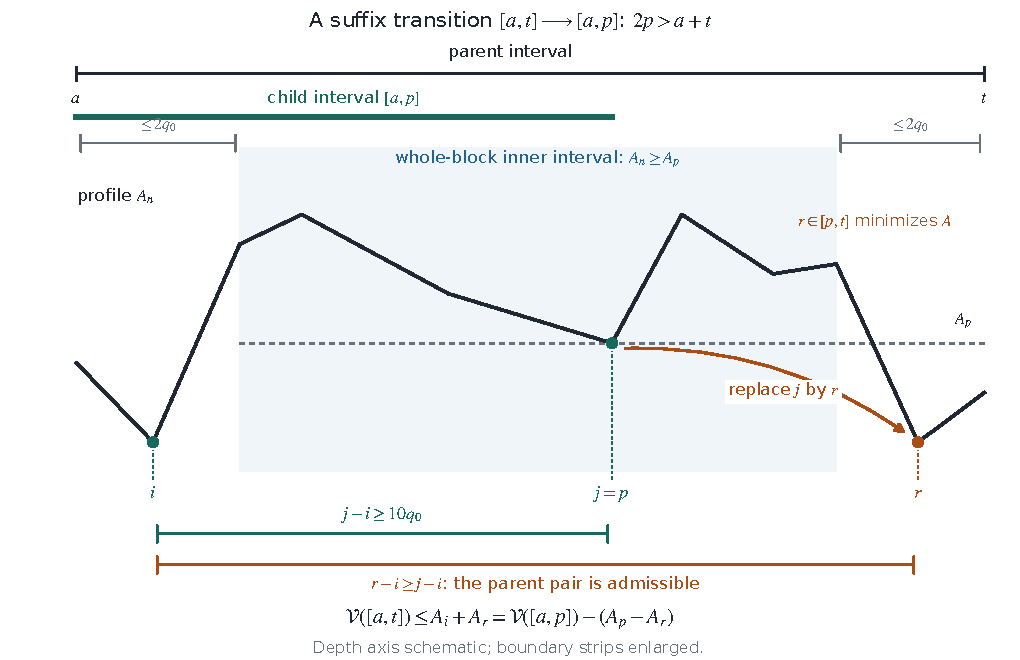
\includegraphics[width=\textwidth]{figures/potential-replacement.pdf}
 \caption{Payment for a suffix transition in Lemma~\ref{ledger:payment}.
 Replacing the later depth of a minimizing child pair by the inner-interval
 minimizer $p$ preserves separation and cannot increase the sum. Thus a
 minimizing child pair can be chosen as $(i,p)$. If $r$ minimizes $A$ on
 $[p,t]$, the pair $(i,r)$ is
 admissible in the parent. Its sum is lower by $A_p-A_r$, which pays the
 transition cost. A positive drop places $r$ beyond the inner interval.
 The depth axis is schematic, with the boundary strips enlarged.}
 \label{fig:potential-replacement}
\end{figure}


\begin{lemma}[Finite policy and smoothing budget]\label{ledger:termination}
Every branch of the state reductions has at most \(20/\kappa\)
non-low transitions and at most \(1/\sigma\) low transitions, for
sufficiently small fixed parameters and sufficiently large \(N\).
Along such a branch the smoothing index increases by at most
\(20/\kappa+1/\sigma\).  If the initial index is zero, every index
required by the iteration, including the next support level used by
a mask, is less than
\[
 J_0=\left\lceil100(1/\kappa+1/\sigma)+100\right\rceil.
\]
\end{lemma}

\begin{proof}
Along a branch the start depth never decreases and the end depth
never increases.  Let \(K\) be the number of fixed block
representatives; for large \(N\), \(K\le1/\kappa+2\).
Every high or direct step strictly advances the start to a
representative.  Such a representative can never be passed twice,
so together these steps number at most \(K\).  Each suffix step
lowers the end by at least \(q_0\), and therefore there are at most
\(N/q_0\le1/\kappa\) suffix steps.  Low steps lower the end by
at least \(\sigma N\), so there are at most \(1/\sigma\).

An angular episode starts at the root or immediately after a high
step and ends at a far step or a stopping term.  Direct and near
steps remain in that episode.  There are at most \(K+1\) episodes,
and hence at most \(K+1\) far steps.

Consider a near step whose child is nonterminal.  That child has
width \(2L_0>100q_0\), so the floor in the formula for \(L_0\)
is inactive and \(L=L_0\).  Remove the factors whose anchors have
now been reached.  If the maximum remaining nominal length
decreases, at least one formerly maximal anchor has just been
passed; charge the near step to one such anchor.  These charges
are distinct along the branch.  If the maximum stays equal to
\(L\), recomputing \(v-2L\) at the child gives exactly its start
depth, so the very next step is direct.  Charge this near step to
that next direct step.  Finally there is at most one near step
with terminal child.  Thus near steps number at most \(2K+1\).
The combined non-low count is at most \(5K+2\), which is less
than \(20/\kappa\) for sufficiently small \(\kappa\).

Only suffix, low, and far steps increase the smoothing index;
each increases it by one.  If \(i_{\mathrm{in}}\) is the initial
index, the preceding counts therefore give
\[
 i\le i_{\mathrm{in}}+20/\kappa+1/\sigma
\]
at every state on the branch.  High, direct, and near steps use the
level-\(i+1\) supports of their index-\(i\) symbols without increasing
the index.  For \(i_{\mathrm{in}}=0\), even this additional support
level remains below \(J_0\), since
\(20/\kappa+1/\sigma+1<J_0\).  Thus every mask and support level
required for the iteration from index zero is available.
\end{proof}

\begin{theorem}[Single-profile angular bound]\label{ledger:bound}
Let \(\mathsf H_0^{[c,N]}(c,N)\) be a recursive angular state of
nonterminal width, as in Definition~\ref{rec:angular-state}.
Fix its initial derivative budget \(B\) and its common numerical angular
bounds \(Q_j\), independently of \(N\), as in
Definition~\ref{osc:symbols}.
Then
\begin{equation}\label{ledger:bound-equation}
 \mathsf H_0^{[c,N]}(c,N)
 \le R^{2A_c-\mathcal V([c,N])
                   +C_d(\kappa+\sigma/\kappa)+o(1)}.
\end{equation}
This bound holds uniformly over its two occupied cells, including
two copies of the same cell, and over its admissible bounded
spatial multipliers and symbols with these fixed bounds.  The \(o(1)\)
term may depend on \(B\) and the \(Q_j\).
\end{theorem}

\begin{proof}
Iterate Proposition~\ref{rec:reductions}, stopping at every terminal
state or low-frequency stopping term.  Lemma~\ref{ledger:termination}
gives a depth bound depending only on the fixed parameters.  Since the
root index is zero, it also ensures that every index required to continue
a nonterminal child is available.
Each transition has at most polynomially many discrete choices
in \(N\), and all coefficient sums in the oscillatory estimates
are bounded or subpower.  Thus the total main term is bounded by
\(R^{o(1)}\) times the largest terminal branch bound.  Suprema
over symbol classes are already part of the transition bounds
and require no count of the members of those classes.

Fix a branch, and let \(a_f\) be its final start.  The changes
of start in \eqref{rec:transition-factor} telescope exactly to
\(2A_c-2A_{a_f}\).  By Lemma~\ref{ledger:payment}, all costs
are bounded by increases in the potential while it is defined.
If a child has width less than \(10q_0\), it is already terminal;
moreover, the step reaching it has zero cost, since every
potentially positive-cost child has width greater than
\(10q_0\).  Let \(J_*=[u,w]\) be the last interval on the
branch with defined potential.  Then
\begin{equation}\label{ledger:cost-sum}
 \sum\mathrm{cost}
 \le\mathcal V(J_*)-\mathcal V([c,N]).
\end{equation}
This also applies when a low-frequency term stops at a
nonterminal interval.

We estimate \(\mathcal V(J_*)\) directly; no potential is assigned
to a shorter final interval.  Nesting gives \(a_f\in[u,w]\), and
\(w-u\ge10q_0\).  Set
\[
 i=\max\{u,\min\{a_f,w-10q_0\}\},\qquad j=i+10q_0.
\]
Both indices lie in \(J_*\), they are separated by \(10q_0\),
and each is within \(10q_0\) of \(a_f\).  The profile Lipschitz
bound therefore gives
\begin{equation}\label{ledger:last-potential}
 \mathcal V(J_*)\le A_i+A_j
 \le2A_{a_f}+20d\,q_0/N
 =2A_{a_f}+O_d(\kappa)+o(1).
\end{equation}
Combining \eqref{ledger:cost-sum}--\eqref{ledger:last-potential}
with the telescoping start factors leaves
\(2A_c-\mathcal V([c,N])+O_d(\kappa)+o(1)\).
The stopping bound contributes \(O_d(\kappa+\sigma)\).
Only non-low transitions incur \(C_d\sigma\) slack, so their
combined loss is \(O_d(\sigma/\kappa)\), by
Lemma~\ref{ledger:termination}.  Low transitions contribute only
subpower factors.  This proves the main-term estimate in
\eqref{ledger:bound-equation}.

For completeness, we fix the error and derivative budgets before
taking \(N\) large.  Since \(m\) is nondecreasing and
\(d\)-Lipschitz with \(m(0)=0\), all differences of \(A\) and
all costs in the reductions are bounded in absolute value by a
dimensional constant.  Each ancestor main factor is consequently
at most \(R^{C_d+o(1)}\).  Choose a target accuracy
\[
 T>C_d(1/\kappa+1/\sigma)+10d+10,
\]
with the dimensional constant large enough for the branch bound.
Demand this accuracy after all single-step normalizations and
sums.  Lemma~\ref{ledger:termination} then ensures that every
propagated additive error is negligible relative to the right
side of \eqref{ledger:bound-equation}.

There is no recursive increase of the persistent angular
derivative budget.  Each passage from a positive distance count
to an angular state begins with fresh undifferentiated masks;
choose its inverse stationary expansion order first, large
enough for the prescribed \(T\).  The resulting finite order,
together with the initial order in the Theorem, bounds all
derivatives carried by angular states.  The common bounds for the smooth
angular factors can likewise be fixed from the initial \(Q_j\) and the
bounds in Proposition~\ref{osc:shell-conversion} at the fixed accuracy
used for these conversions.
The graph estimate returns the original symbols restricted to child cells,
with no additional derivatives.  Removing reached
factors from its positive child energy, as in a near transition, adds
no derivatives to the remaining symbols.  A far step may use
an arbitrarily long direct stationary expansion, but its child
is a positive distance count and carries none of those
derivatives.  Choose the nonstationary integration orders and
the direct stationary orders after this persistent budget has
been fixed.  They may depend on \(d,\kappa,\sigma,T\) and the
initial budget, but not on \(N\).  Their large constants and
polynomial descriptor counts are absorbed in the permitted
constant and \(o(1)\) terms; the dimensional exponent losses in
the preceding algebra are unchanged.  The asserted bound
follows.
\end{proof}

\section{Entry, shell summation, and the limiting distance measure}
\label{asm:section}
\label{sec:assembly}

The graph estimate and the two-depth potential now give decay on each frequency
shell.  The measures used on different shells have different classes and
masks.  We first explain how to restore their mass, and then give a scalar
reconstruction argument that accommodates the decreasing pair filters.
Throughout this Section all distances are measured in the original
space $\R^d$.

\subsection{The entry depth}

Let $S=d/2$.  Fix the starting probabilities $\mu_1,\mu_2$ and the number
$\chi>0$ supplied by Proposition~\ref{prep:starting-pairs}.
Make one common similarity placing $E$ in $(1/4,3/4)^d$, and retain
the notation for the transformed sets and measures.  This multiplies
every distance by one fixed positive constant and preserves the
desired positive-measure conclusion.  Choose one small common
translation of the dyadic grid whose boundaries have zero mass for
both starting laws.  Its depth-zero cube $Q_0$ still contains $E$ in
its interior.  Use this same grid for both class decompositions.
The two actual supports remain separated by a fixed positive
distance, and their cross directions remain in the prepared patch.
At scale
$R=2^N$, apply Lemma~\ref{reg:regularization} with parameter $\sigma$ to
both probabilities.  Write $\mathcal C_{j,N}$ for the retained classes on
side $j$.  For $C\in\mathcal C_{j,N}$, let
\[
 a_{j,C}=\mu_j(C),\qquad
 \rho_{j,C}=a_{j,C}^{-1}\mu_j|_C.
\]
The classes on each side are disjoint, their number is $R^{o(1)}$, and
their discarded original mass is at most $R^{-\sigma+o(1)}$.  All the
$o(1)$ terms below are uniform over these classes, with the fixed
parameters held constant.
Every normalized class is supported in the same root cube $Q_0$ and
assigns it mass one.  Since every profile has $m_j(0)=0$, its root
normalization is exactly $M_j(0)=R^{-m_j(0)}=1$.

For a pair of classes, suppress their labels and write
\[
 A_{j,n}=m_j(n/N)-Sn/N,\qquad
 k_j(g,p)=A_{j,p}-\min_{g\le n\le p}A_{j,n}.
\]
Recall from Lemma~\ref{test:profile-bounds} that
\begin{equation}
 \label{asm:profile-input}
 A_{j,0}=0,\qquad
 |A_{j,n}-A_{j,n'}|\le d|n-n'|/N,\qquad
 A_{j,n}\ge\chi n/N-C_d\sigma.
\end{equation}
Here and in what follows, constants denoted by $C_d$ may be enlarged a
finite number of times and depend only on $d$.

We seek a common depth $c$ for which one entry cost $k_j(0,c)$ is small
and both excess profiles remain above a positive level on $[c,N]$.
The graph estimate contributes the smaller cost.  After
Cauchy--Schwarz separates the profiles, the two single-profile
estimates must supply a larger potential saving.

\begin{lemma}[Entry depth]\label{asm:entry}
Fix $0<\beta<\min(\chi/10,1/10)$.  If $\sigma$ is sufficiently small
in terms of $d,\chi,\beta$, then, for all sufficiently large $N$, the
integer
\begin{equation}
 \label{asm:entry-definition}
 c=\max\{n\in\{0,\ldots,N\}:
                  \min(A_{1,n},A_{2,n})\le\beta\}
\end{equation}
is defined and satisfies
\begin{align}
 \label{asm:entry-range}
 &\left\lfloor\frac{\beta N}{2d}\right\rfloor\le c<N/4,\\
 \label{asm:entry-lower}
 &A_{j,n}\ge\beta-d/N
       \quad(j=1,2,\ c\le n\le N),\\
 \label{asm:entry-cost}
 &\min_{j=1,2} k_j(0,c)\le\beta+C_d\sigma.
\end{align}
If $\kappa$ is sufficiently small and $q_0=\lceil\kappa N\rceil$, the
interval $[c,N]$ is nonterminal.  Its potentials from
Definition~\ref{ledger:potential} obey
\begin{equation}
 \label{asm:entry-potential}
 \mathcal V_j([c,N])
 :=\min_{\substack{c\le u<v\le N\\v-u\ge10q_0}}
                         (A_{j,u}+A_{j,v})
 \ge2\beta-2d/N.
\end{equation}
\end{lemma}

\begin{proof}
The index $0$ qualifies in Equation~\eqref{asm:entry-definition}.
For $n\le\beta N/(2d)$, the Lipschitz bound in
Equation~\eqref{asm:profile-input} gives $A_{j,n}\le\beta/2$, proving
the lower bound in Equation~\eqref{asm:entry-range}.  For $n\ge N/4$,
the lower profile bound gives
$A_{j,n}\ge\chi/4-C_d\sigma>\beta$ when $\sigma$ is sufficiently
small.  This proves its upper bound.

By maximality of $c$, both $A_{j,c+1}$ exceed $\beta$, so
$A_{j,c}>\beta-d/N$.  Both profiles exceed $\beta$ at every later
index.  For at least one side $j_*$, we also have
$A_{j_*,c}\le\beta$.  Since
$\min_{0\le n\le c}A_{j_*,n}\ge-C_d\sigma$, this gives
Equation~\eqref{asm:entry-cost}.  The width of $[c,N]$ exceeds $3N/4$;
thus it exceeds $100q_0$ for sufficiently small fixed $\kappa$ and
large $N$.  Every pair entering its potential consists of two indices
covered by Equation~\eqref{asm:entry-lower}, which proves
Equation~\eqref{asm:entry-potential}.
\end{proof}

\subsection{Positive approximants and restoration of mass}

Write
\[
 D(x,y)=|x-y|,\qquad e(x,y)=\frac{x-y}{|x-y|},\qquad
 W(x,y)=D(x,y)^{-(d-1)/2}.
\]
The fixed separated supports give constants $0<d_0<d_1<\infty$ with
\begin{equation}
 \label{asm:distance-range}
 d_0\le D(x,y)\le d_1
 \quad\hbox{on }\supp\mu_1\times\supp\mu_2.
\end{equation}
In particular $W$ is bounded above and below there by positive constants.

For each pair of classes $(C_1,C_2)$, use its own entry index $c$ from
Equation~\eqref{asm:entry-definition}.  At endpoint $j$ take the extra
parallel descriptor $[0,c]$, together with every descriptor in
$\mathcal M_j(c,N)$.  Let
\begin{equation}
 \label{asm:endpoint-mask}
 b_{j;C_1,C_2}(z,w)
 =w^{(j)}_{0,[0,c]}(z,w)
                  \prod_{\mathfrak t\in\mathcal M_j(c,N)}
                         w^{(j)}_{0,\mathfrak t}(z,w).
\end{equation}
The masks are those of Lemma~\ref{test:smooth-masks}; thus every factor
lies in $[0,1]$ and equals one when its level-zero condition holds.
Antipodal symmetry allows both endpoints to be evaluated at $e(x,y)$.
Define the Borel function $\Theta_N$ on the fixed separated product
$E_1\times E_2$ by
\[
 \Theta_N(x,y)=
 b_{1;C_1,C_2}(x,e(x,y))
 b_{2;C_1,C_2}(y,e(x,y))
 \quad\hbox{if }(x,y)\in C_1\times C_2,
\]
and set it equal to zero whenever either endpoint belongs to no retained
class.
In particular $0\le\Theta_N\le1$.

Let $\Gamma_N$ be the decreasing pair filters of
Proposition~\ref{prep:starting-pairs}.  With $D_\#$ denoting pushforward
under the scalar map $D$, define
\begin{equation}
 \label{asm:measures}
 \alpha_N=D_\#\bigl(W\one_{\Gamma_N}
                          (\mu_1\otimes\mu_2)\bigr),\qquad
 \tau_N=D_\#\bigl(W\one_{\Gamma_N}\Theta_N
                          (\mu_1\otimes\mu_2)\bigr).
\end{equation}
These measures use the original class masses.  Only $\tau_N$ depends on
the shell's class decomposition and angular masks.

\begin{lemma}[Restoration of mass]\label{asm:retained-measures}
There is $\eta>0$, depending on the fixed parameters and starting
measures, such that
\begin{equation}
 \label{asm:tv-approximation}
 0\le\tau_N\le\alpha_N,\qquad
 \|\alpha_N-\tau_N\|_{\TV}\lesssim2^{-\eta N}.
\end{equation}
Moreover $\alpha_N$ decreases to the nonzero finite positive measure
\begin{equation}
 \label{asm:limit-measure}
 \alpha_\infty=D_\#\bigl(W\one_{\Gamma_\infty}
                               (\mu_1\otimes\mu_2)\bigr),\qquad
 \Gamma_\infty=\bigcap_N\Gamma_N.
\end{equation}
All these measures are carried by the compact set of original distances
$\Delta(E)$.
\end{lemma}

\begin{proof}
Apply the cap preparation in Proposition~\ref{prep:starting-pairs} with
loss $R^\sigma$.  It gives $\mathcal G_N\subset\Gamma_N$ such that
\[
 (\mu_1\otimes\mu_2)(\Gamma_N\setminus\mathcal G_N)
       \lesssim R^{-c_*}
 \quad\hbox{for some }c_*>0.
\]
For $\mu_1$-almost every first endpoint $x$, the angular subprobability
\[
 \xi_{N,x}=e(x,\cdot)_*
             \bigl(\one_{\mathcal G_N}(x,\cdot)\mu_2\bigr)
\]
has the required $S$-cap bound with loss $R^\sigma$ down to scale
$R^{-1}$.  The change from $\pi_x(y)$ to $e(x,y)=-\pi_x(y)$ preserves
cap bounds, since the antipodal map sends caps to caps.  The analogous
assertion holds for $\mu_2$-almost every second endpoint with the
endpoints reversed.
These are bounds for restrictions of the original opposite probability.

Fix $C_1,C_2$ and one descriptor $\mathfrak t$ used at the first endpoint.
For $\mu_1$-almost every $x\in C_1$, the anchor cell determined by
$\mathfrak t$ and $x$ is occupied and $\xi_{N,x}$ has the cap bound above.  Let
$F_{C_1,C_2,\mathfrak t,x}$ be the directions failing this level-zero test.
For such $x$, Lemma~\ref{test:exceptional-directions} applies directly
to $\xi_{N,x}$ and gives
\begin{equation}
 \label{asm:original-fiber-estimate}
 \mu_2\{y\in C_2:(x,y)\in\mathcal G_N,
       \ e(x,y)\in F_{C_1,C_2,\mathfrak t,x}\}\le R^{-\sigma}.
\end{equation}
Restricting the set of $y$ to $C_2$ only decreases the left side; no
normalization by $\mu_2(C_2)$ occurs.  Integrating in $x$ over $C_1$
costs at most $a_{1,C_1}R^{-\sigma}$.  Sum first over $C_1$, whose
original masses have sum at most one, and then over $C_2$ and the
descriptors.  The latter two counts are $R^{o(1)}$, by
Lemma~\ref{reg:regularization} and
Lemma~\ref{test:descriptor-properties}.  Thus the first-endpoint
failure mass is $R^{-\sigma+o(1)}$.  The same argument in the other
orientation gives this bound for second-endpoint failures.  There is
no sum over anchor cells: a point and descriptor already specify one.

The product in Equation~\eqref{asm:endpoint-mask} equals one if all
its level-zero tests hold.  Hence $1-\Theta_N$ on retained class pairs is
bounded by the indicator of the union of these failures.  Including
the original mass outside retained class pairs and
$\Gamma_N\setminus\mathcal G_N$ gives
\[
 \int_{\Gamma_N}(1-\Theta_N)\,d(\mu_1\otimes\mu_2)
 \lesssim R^{-c_*}+R^{-\sigma+o(1)}.
\]
The bounded weight $W$ proves Equation~\eqref{asm:tv-approximation},
for example with any fixed
$0<\eta<\min(c_*,\sigma)/2$ and sufficiently large $N$.
The set $\mathcal G_N$ was used only in this estimate: it is not a
multiplier in Equation~\eqref{asm:measures}.

The filters $\Gamma_N$ decrease and have positive limiting product
mass.  Continuity of a finite measure along decreasing sets proves
Equation~\eqref{asm:limit-measure} and monotonicity of $\alpha_N$.
The positive lower bound for $W$ shows
$\alpha_\infty(\R)>0$.  Finally, the two original supports are compact
subsets of $E$, and $D$ is continuous.  Every pushforward above is
therefore carried by their compact distance image, which is contained
in $\Delta(E)$.
\end{proof}

\subsection{The shell estimate}

\begin{proposition}[Decay of the approximating distance measures]
\label{asm:shell-decay}
The fixed parameters can be chosen, in the order
$\beta,\kappa,\sigma,\omega$, so that some $\gamma>0$ satisfies
\begin{equation}
 \label{asm:shell-bound}
 \int_{2^{N-1}\le |r|\le2^{N+1}}
                   |\widehat{\tau_N}(r)|^2\,dr
       \lesssim2^{-\gamma N}
\end{equation}
for all sufficiently large $N$.
\end{proposition}

\begin{proof}
For the moment fix one normalized class pair and one product
$X_\ell\times Y_\ell$ in the spatial partition of $\Gamma_N$.
The corresponding component measure $\nu$ is the pushforward of
\[
 W(x,y)\one_{X_\ell}(x)\one_{Y_\ell}(y)
 b_{1;C_1,C_2}(x,e(x,y))b_{2;C_1,C_2}(y,e(x,y))
             \,d\rho_{1,C_1}(x)\,d\rho_{2,C_2}(y).
\]
The product indicators are permitted bounded measurable spatial
multipliers in the oscillatory estimates.  At depth zero take
$X=Y=Q_0$, each with its own normalized class law.  These are occupied
root cells, with $M_1(0)=M_2(0)=1$.  Their supported laws lie in the
fixed separated sets $E_1,E_2$, so the outer-support geometry of
Section~\ref{osc:section} applies.  The cell-center separation in
Equation~\eqref{osc:separation} is the internal-cell convention; the
outer root uses the separation of the supported laws.  In particular,
all root spatial diameters in the graph argument are $O_d(1)$, while
the actual cross distances have a fixed positive lower bound.
By
Lemma~\ref{test:descriptor-properties}, the largest nominal length
of an endpoint descriptor is at most
\[
 L\le\max\bigl(c,(N-c)/2\bigr)\le N/2.
\]
Thus the root shell conversion, Proposition~\ref{osc:shell-conversion},
applies with $a=0$, $v=N$.  Its weight is precisely $W$; there is no
internal normalization of the distance weight at this root.  For any
prescribed fixed $T>0$, it bounds the squared Fourier norm on the positive
shell by $R^{o(1)}\sup\mathsf H_F(0,N)+O(R^{-T})$.  The supremum retains
the root cells, class normalizations, lists, and smoothing index zero;
its admissible symbols have the fixed derivative budget and common
numerical angular bounds supplied by that Proposition for $T$.

Apply Corollary~\ref{graph:separated-form} at $p=c$ to each energy in this
supremum.  The required parallel
descriptor is the extra $[0,c]$ on each side, with $g=0$.  All scale
conditions hold: $c>0$ for large $N$, $c<N/4$,
$L\le N/2<N-c$, and $N-c\ge10\sigma N$.  Since $A_{j,0}=0$, the
graph factor is
\begin{equation}
 \label{asm:graph-factor}
 R^{-A_{1,c}-A_{2,c}+\min_j k_j(0,c)+O_d(\sigma)+o(1)}.
\end{equation}
The graph estimate produces a general two-profile energy
$\mathsf H(c,N)$ on a pair of occupied $c$-cells, still carrying the
same endpoint symbols.

On these cells the extra $[0,c]$ factor is spatially constant within
each endpoint cell.  It, and any of its normalized differentiated
versions produced by shell conversion, can be removed at bounded
cost from the positive independent angular energies.  The remaining
descriptor lists are exactly those with base $[c,N]$ and with reached
anchors omitted.  This removal is made in the general positive energy
$\mathsf H$, where the two angular factors are nonnegative.

To separate the two profiles, write their nonnegative angular
energies as $E_1(r),E_2(r)$ and use the common measure
$d\lambda_N(r)=\Psi(r/2^N)\,dr/2^N$.  Cauchy--Schwarz gives the exact
normalization
\begin{equation}
 \label{asm:two-profile-cs}
 \begin{split}
 2^{d(N-c)}\int E_1(r)E_2(r)\,d\lambda_N(r)
 &\le
 \left(2^{d(N-c)}\int E_1(r)^2\,d\lambda_N(r)\right)^{1/2}\\
 &\quad\cdot
 \left(2^{d(N-c)}\int E_2(r)^2\,d\lambda_N(r)\right)^{1/2}.
 \end{split}
\end{equation}
Each parenthesis is the independent angular energy formed by
duplicating one endpoint law, cell, and symbol.  With the unreached
descriptors of $\mathcal M_j(c,N)$, it is the single-profile recursive
state $\mathsf H_0^{[c,N]}(c,N)$ for profile $j$; denote this value by
$\mathsf H_j(c,N)$.  Its symbols have the fixed derivative budget and
common numerical angular bounds supplied by shell conversion;
restriction to the $c$-cells and duplication preserve these bounds.
These states impose no separation condition, so
Theorem~\ref{ledger:bound} applies to each, including the case of two
identical cells.  It yields
\[
 \mathsf H_j(c,N)
 \le R^{2A_{j,c}-\mathcal V_j([c,N])
                         +O_d(\kappa+\sigma/\kappa)+o(1)}.
\]
The profile terms in Equation~\eqref{asm:graph-factor} and the
geometric mean of these bounds combine to
\begin{equation}
 \label{asm:entry-cancellation}
 \begin{split}
 &-A_{1,c}-A_{2,c}+\min_j k_j(0,c)
       +\frac12\sum_{j=1}^2
                    \bigl(2A_{j,c}-\mathcal V_j([c,N])\bigr)\\
 &\hspace{20mm}
 =\min_j k_j(0,c)-\frac12
                     \bigl(\mathcal V_1([c,N])+\mathcal V_2([c,N])\bigr)
 \le-\beta+C_d\sigma+2d/N,
 \end{split}
\end{equation}
where the last inequality uses the cost and potential bounds in
Lemma~\ref{asm:entry}.  Including the stated losses proves uniformly
for each component that
\begin{equation}
 \label{asm:component-shell}
 \int_{2^{N-1}\le r\le2^{N+1}}|\widehat\nu(r)|^2\,dr
 \lesssim
 R^{-\beta+C_d(\kappa+\sigma/\kappa)+o(1)}+R^{-T}.
\end{equation}
Here $T$ can be any fixed sufficiently large number, after choosing
the expansion and integration-by-parts orders.  The term $O_d(\sigma)$
has been included in $O_d(\sigma/\kappa)$, with $\kappa<1$.

We make the parameter and error choices explicit.  First choose
$\beta$ as in Lemma~\ref{asm:entry}.  Next choose $\kappa$ so small
that the entry interval is nonterminal and
$C_d\kappa<\beta/16$.  Then choose $\sigma$ so small that all the
profile and transition hypotheses hold and
$C_d\sigma/\kappa<\beta/16$.  Finally choose $\omega>0$ so small
that
\begin{equation}
 \label{asm:omega-choice}
 4d\omega<\beta/8.
\end{equation}
The preparation of $\Gamma_N$ is used with this fixed $\omega$ and
cap loss $R^\sigma$.  Its deletion exponent $c_*$ may depend on both
parameters; only $c_*>0$ was needed in
Lemma~\ref{asm:retained-measures}.

For completeness, the error accuracy is fixed after these parameters
and before $N$ tends to infinity.  Theorem~\ref{ledger:bound} bounds
the number of steps on a branch by a constant depending on
$\kappa,\sigma$.  Choose a fixed local negative-power accuracy large
enough to dominate all ancestor factors and all errors on such a
branch, leaving the root remainder $R^{-T}$ in
Equation~\eqref{asm:component-shell}, with, say, $T>10+4d\omega$.
The inverse expansion orders are then fixed and determine a finite
symbol derivative budget.  The direct expansion and
integration-by-parts orders are chosen for that budget and accuracy,
as in Theorem~\ref{ledger:bound}.  The graph step and
Equation~\eqref{asm:two-profile-cs} introduce no persistent new
derivative orders; the spatial indicators have zero angular
derivatives.  These choices affect constants and the threshold for
$N$, and do not change the dimensional coefficients in the exponent
losses above.  We now take $N$ sufficiently large for all these fixed
choices and for the uniform $o(1)$ losses.

There are at most $L_N\lesssim R^{2d\omega}$ spatial products in
$\Gamma_N$.  Let $\nu_{C_1,C_2,\ell}$ denote the preceding component.
The exact recombination is
\[
 \tau_N=\sum_{C_1,C_2}a_{1,C_1}a_{2,C_2}
                    \sum_{\ell=1}^{L_N}\nu_{C_1,C_2,\ell}.
\]
Triangle inequality in the Fourier $L^2$ norm costs no class-count
factor, because
\[
 \sum_{C_1,C_2}a_{1,C_1}a_{2,C_2}
 =\left(\sum_{C_1}a_{1,C_1}\right)
  \left(\sum_{C_2}a_{2,C_2}\right)\le1.
\]
It costs at most $L_N$ for the spatial products.  Squaring therefore
costs $R^{4d\omega}$, giving
\begin{equation}
 \label{asm:assembled-shell}
 \int_{2^{N-1}\le r\le2^{N+1}}
                  |\widehat{\tau_N}(r)|^2\,dr
 \lesssim R^{-\beta+C_d(\kappa+\sigma/\kappa)+4d\omega+o(1)}
                       +R^{-T+4d\omega}.
\end{equation}
Our successive choices leave a strictly negative exponent; for
example, increasing the starting $N$ if necessary, the right side is
$O(R^{-\beta/2})$.  Each $\tau_N$ is a real positive measure, so
$\widehat{\tau_N}(-r)=\overline{\widehat{\tau_N}(r)}$.  The same
bound holds on the negative shell, proving
Equation~\eqref{asm:shell-bound} with some $\gamma>0$.
\end{proof}

\subsection{A monotone shell reconstruction lemma}

The following scalar fact isolates the final limiting argument.  Its
hypotheses require no rate at which the decreasing measures approach
their limit.  The proof combines a smooth dyadic Fourier decomposition
with the summable positive increments of a decreasing family of finite
measures. We give this reconstruction explicitly.

\begin{lemma}[Monotone measure shell criterion]\label{asm:monotone-shell}
Let $(\alpha_N)_{N\ge K}$ be finite positive Borel measures on $\R$
with $\alpha_{N+1}\le\alpha_N$, and let
$\alpha_\infty=\lim_N\alpha_N$.  Let $\tau_N$ be finite complex
Borel measures such that
\begin{equation}
 \label{asm:criterion-hypotheses}
 \sum_{N\ge K}\|\alpha_N-\tau_N\|_{\TV}<\infty,
 \qquad
 \sum_{N\ge K}
 \left(\int_{2^{N-1}\le |r|\le2^{N+1}}
                   |\widehat{\tau_N}(r)|^2\,dr\right)^{1/2}<\infty.
\end{equation}
Then $\alpha_\infty$ is absolutely continuous with respect to
Lebesgue measure.  In particular, the conclusion holds if the two
quantities inside these sums are respectively
$O(2^{-\eta N})$ and $O(2^{-\gamma N/2})$ for arbitrary
$\eta,\gamma>0$.
\end{lemma}

\begin{proof}
Choose $\vartheta\in C_c^\infty(\R)$ equal to one on $[-1,1]$ and
supported in $[-2,2]$.  Let $Q_N$ be convolution with the inverse
Fourier transform of $\vartheta(2^{-N}r)$, and put
$P_N=Q_N-Q_{N-1}$.  The multiplier of $P_N$ is supported in
$\{2^{N-1}\le|r|\le2^{N+1}\}$.  Dilation of the fixed Schwartz
kernel gives a constant $C_\vartheta$ such that, for every finite
measure $\nu$,
\begin{equation}
 \label{asm:low-cutoff-bound}
 \|Q_N\nu\|_{L^1}\le C_\vartheta\|\nu\|_{\TV},\qquad
 \left\|\sum_{N=a}^bP_N\nu\right\|_{L^1}
 \le2C_\vartheta\|\nu\|_{\TV}\quad(a\le b).
\end{equation}
The second bound follows from telescoping to $Q_b-Q_{a-1}$; in
particular its constant is independent of the number of bands.

With the convention $\widehat\nu(r)=\int e^{-irt}\,d\nu(t)$,
Plancherel \cite[equation~(12.4)]{Mattila1995} and the uniformly
bounded band multipliers give
\[
 \|P_N\tau_N\|_{L^2}
 \lesssim
 \left(\int_{2^{N-1}\le |r|\le2^{N+1}}
                   |\widehat{\tau_N}(r)|^2\,dr\right)^{1/2}.
\]
Thus
\begin{equation}
 \label{asm:two-convergent-series}
 G:=\sum_{N\ge K}P_N\tau_N\quad\hbox{converges in }L^2,
 \qquad
 H:=\sum_{N\ge K}P_N(\alpha_N-\tau_N)
                         \quad\hbox{converges in }L^1.
\end{equation}
Both series converge absolutely in the indicated Banach space.

It remains to account for the variation of $\alpha_N$.  Set
$\zeta_n=\alpha_n-\alpha_{n+1}\ge0$.  Monotonicity and finiteness
give
\begin{equation}
 \label{asm:measure-telescoping}
 \sum_{n\ge K}\|\zeta_n\|_{\TV}
       =\alpha_K(\R)-\alpha_\infty(\R)<\infty,
 \qquad
 \alpha_N-\alpha_\infty=\sum_{n\ge N}\zeta_n
                         \quad\hbox{in total variation}.
\end{equation}
For a finite $M\ge K$, define
$Z_M=\sum_{N=K}^MP_N(\alpha_N-\alpha_\infty)$.  Substituting
Equation~\eqref{asm:measure-telescoping} into this finite sum and
using the bounded operators from measures to $L^1$ gives the exact
identity
\begin{equation}
 \label{asm:finite-band-identity}
 Z_M=\sum_{n\ge K}
             (Q_{\min(n,M)}-Q_{K-1})\zeta_n.
\end{equation}
For each fixed $M$ the series on the right converges in $L^1$.
Moreover, Equation~\eqref{asm:low-cutoff-bound} shows that
\[
 Z:=\sum_{n\ge K}(Q_n-Q_{K-1})\zeta_n
\]
converges absolutely in $L^1$.  Subtracting the two series cancels
all $n\le M$, and gives
\begin{equation}
 \label{asm:variation-tail}
 \begin{split}
 \|Z_M-Z\|_{L^1}
 &\le2C_\vartheta\sum_{n>M}\|\zeta_n\|_{\TV}\\
 &=2C_\vartheta
             \|\alpha_{M+1}-\alpha_\infty\|_{\TV}
 \longrightarrow0.
 \end{split}
\end{equation}
This is where monotonicity is used.  The original double series has
not been rearranged without a convergence justification.

Finally, finite telescoping gives
\begin{equation}
 \label{asm:reconstruction}
 Q_M\alpha_\infty
 =Q_{K-1}\alpha_\infty
  +\sum_{N=K}^MP_N\tau_N
  +\sum_{N=K}^MP_N(\alpha_N-\tau_N)-Z_M.
\end{equation}
The fixed low-frequency term $Q_{K-1}\alpha_\infty$ is a smooth
$L^1$ function by convolution with a Schwartz kernel.  By
Equations~\eqref{asm:two-convergent-series} and
\eqref{asm:variation-tail}, the right side converges in
$L^1+L^2$, hence in distributions, to
\[
 f=Q_{K-1}\alpha_\infty+G+H-Z\in L^1_{\mathrm{loc}}(\R).
\]
The kernels defining $Q_M$ form an approximate identity, so the
left side of Equation~\eqref{asm:reconstruction} converges in
distributions to $\alpha_\infty$.  Therefore
$\alpha_\infty=f\,\cL^1$.  Since $\alpha_\infty$ is a finite
positive measure, this locally integrable density is nonnegative
almost everywhere and belongs to $L^1(\R)$.  This proves absolute
continuity.
\end{proof}

\subsection{Completion of the proof}

\begin{proposition}\label{asm:completion}
For the starting pair in Proposition~\ref{prep:starting-pairs}, there
is a nonzero finite positive measure, absolutely continuous with
respect to $\cL^1$, carried by the original distance set $\Delta(E)$.
Consequently $\cL^1(\Delta(E))>0$.
\end{proposition}

\begin{proof}
Choose the parameters as in Proposition~\ref{asm:shell-decay}.
Lemma~\ref{asm:retained-measures} gives decreasing $\alpha_N$ with
nonzero limit $\alpha_\infty$, and approximants $\tau_N$ with
summable total-variation error.  Proposition~\ref{asm:shell-decay}
gives the second summability hypothesis of
Lemma~\ref{asm:monotone-shell}.  That Lemma makes $\alpha_\infty$
absolutely continuous.  By Lemma~\ref{asm:retained-measures} it is
carried by $\Delta(E)$ and has positive mass, so $\Delta(E)$ cannot
be a Lebesgue null set.
\end{proof}

\begin{proof}[Proof of Theorem~\ref{thm:main}]
Start with a Frostman probability on the given compact set
$E\subset\R^d$, $d\ge2$, with exponent strictly larger than $d/2$.
In the odd-dimensional exceptional affine-plane case,
Lemma~\ref{prep:classical-plane} already proves the conclusion using
original distances inside that plane.  In every other case,
Proposition~\ref{prep:starting-pairs} supplies the separated original
probabilities and filters used above, and
Proposition~\ref{asm:completion} proves the conclusion.  This includes
$d=2$: its cap preparation is the integer case of
Lemma~\ref{prep:integer-caps}.  The auxiliary projections used in
preparation control directions only; the measures in
Equation~\eqref{asm:measures} and their nonzero limit are pushforwards
by $|x-y|$ in $\R^d$.  Thus the argument establishes the asserted
positive measure for the original distance set in every dimension
$d\ge2$.
\end{proof}

\bibliographystyle{amsplain}
\bibliography{references}
\end{document}
